\clearpage
\bookpart{概率空间}{Probability Spaces}
\label{part:probability-spaces}

\BookPartGuide{%
卷一用概率表和普通密度计算事件概率、均值与方差，这已经足够处理掷骰、抽检和正态测量。可是很多随机对象既没有概率表，也没有相对于长度的密度：分布可能同时含有点质量和连续部分，观测可能只记录试验结果的一部分，我们还常常需要比较一列随机变量怎样趋于极限。本部分借助上一部分的可测空间、测度、积分与相对密度，把这些问题放进同一个一般概率模型中讨论。

第一章建立一般概率模型：概率空间规定可判断的事件及其概率，随机对象把试验结果送到取值空间，分布记录取值规律，独立性要求联合规律可以分解，期望则是对概率测度的积分。第二章研究只掌握部分信息时的平均与概率，用积分刻画条件期望，再用概率核把各事件的条件概率组织成条件分布，并讨论条件独立怎样简化信息依赖。

后两章研究极限。第三章固定同一个概率空间，比较几乎处处、依概率和平均意义下的收敛，给出交换期望与极限的条件，并由独立部分和的最大偏差与截断证明强大数律。第四章只比较分布，不要求随机变量定义在同一空间上：先建立弱收敛的判据与紧性，再用特征函数识别极限分布，处理联合观测与函数变换后的极限，最后证明中心极限定理。

本部分只讨论单个概率模型中的固定信息与独立序列。信息随时间增长、鞅与随机过程的构造留到卷三，分布之间的距离与比较留到卷四“概率分布”部分，统计推断中的渐近理论留到卷四“推断与因果识别”部分。}

\chapter{一般概率模型与随机对象}
\label{chap:probability-models}

掷两枚骰子，三位记录员各自记下结果：第一位写下两枚骰子的点数，第二位只写点数和，第三位只写点数和是奇是偶。
三份记录来自同一次试验，能回答的问题却不同：只有第一位能判断“第一枚掷出$6$”是否发生，第三位甚至分不清点数和是$7$还是$9$。
再看一个排队的例子：顾客有$40\%$的机会到达时窗口空闲、等待时间恰好为$0$，其余时候等待时间服从指数分布。
这个等待时间既没有概率表，也没有普通密度，它的平均值该怎么算？
还有一个更隐蔽的问题：两个量的概率规律完全相同，它们是否就是“同一个随机变量”？两个量各自的规律都已知，它们一起出现的规律是否也就确定了？

卷一处理概率问题时，计算都落在两种形式上：列出概率表逐项相加，或者写出密度再积分。
上面几个问题说明，这两种形式背后还有几件事没有分开：试验结果本身、我们允许判断的事件、观测到的数值，以及数值的概率规律。
第~\ref{chap:measure-spaces}章已经建立了可测空间、测度、推前和一般积分，本章用这些工具把上述几层分开，使计算不再依赖概率表或密度。

全章沿“结果—观测—规律—累计”的顺序展开。
第~\ref{sec:pmod-probability-space}节把概率模型写成概率空间，并说明零概率事件与“几乎必然”的含义；第~\ref{sec:pmod-random-objects}节把观测写成可测映射，用它生成的$\sigma$代数描述观测带来的信息。
有了观测，第~\ref{sec:pmod-distributions}节把概率从样本空间搬到取值空间，得到分布，并区分“同分布”“几乎处处相等”与联合分布；第~\ref{sec:pmod-independence}节研究联合分布何时分解成各自分布的乘积，这就是独立性。
第~\ref{sec:pmod-expectation}节把求和与密度积分统一成对概率测度的积分，讨论矩条件和几个基本不等式，它们是后面三章研究条件期望和收敛时反复使用的工具。

\section{概率空间}
\label{sec:pmod-probability-space}

一个概率模型不能只列出可能结果。
同一次试验可以按不同精细程度记录，我们必须同时说清：哪些结果可能出现，哪些关于结果的问题允许回答，这些问题的答案各有多大概率。
本节先把这三件事写成概率空间，再处理概率为零的事件。

\subsection{事件与概率模型}

\paragraph{概率模型的三个组成部分}
卷一用样本空间、事件和概率描述随机试验，并要求概率满足非负、总和为$1$与可数可加。
第~\ref{chap:measure-spaces}章的可测空间正好给出“哪些集合允许测量”，测度给出“这些集合各有多大”。
概率模型就是总质量为$1$的测度空间。

\begin{definition}[概率空间]
\label{def:pmod-probability-space}
设$\Omega$是非空集合，$\mathcal F$是$\Omega$上的$\sigma$代数，$\mathbb P:\mathcal F\to[0,1]$是$(\Omega,\mathcal F)$上的测度，并且$\mathbb P(\Omega)=1$。
称三元组$(\Omega,\mathcal F,\mathbb P)$为\term{概率空间}（probability space），称$\Omega$为样本空间，$\mathcal F$中的集合为\term{事件}（event），$\mathbb P$为概率测度。
\end{definition}

定义中$\mathcal F$不能省略。
只有属于$\mathcal F$的集合才有概率，一个$\Omega$的子集若不在$\mathcal F$中，模型就不对它作出任何概率判断。
概率的基本运算规则都直接由测度的性质得到：补事件满足$\mathbb P(\Omega\setminus A)=1-\mathbb P(A)$，$A\subseteq B$时$\mathbb P(A)\le\mathbb P(B)$，任意一列事件满足
\[
  \mathbb P\Bigl(\bigcup_{n=1}^\infty A_n\Bigr)\le\sum_{n=1}^\infty\mathbb P(A_n).
\]
由于总质量有限，事件单调增加或单调减少时，概率都随之收敛到极限事件的概率。
这些结论在第~\ref{chap:measure-spaces}章已经对一般测度成立，这里不再重证；Lebesgue测度的构造也不在本章重复。

\paragraph{同一试验的三种记录}
回到章首的两枚骰子。
样本空间取有序对$\Omega=\{1,\dots,6\}^2$，$36$个结果等可能。
三位记录员保留的信息不同，可以用三个$\sigma$代数表示。

\begin{example}[两枚骰子的三种观测]
\label{ex:pmod-dice-records}
记$\omega=(i,j)$，点数和$S(\omega)=i+j$。
完整记录对应$\mathcal F_{\mathrm{full}}=\mathcal P(\Omega)$，$36$个单点都可以单独判断，共有$2^{36}$个事件。
只记录点数和时，能判断的事件恰好是若干个$\{S=s\}$（$s=2,\dots,12$）的并，记这一族为$\mathcal F_{\mathrm{sum}}$，它有$11$个不可再分的块，共$2^{11}$个事件。
只记录奇偶时，能判断的事件只有
\[
  \mathcal F_{\mathrm{par}}=\bigl\{\varnothing,\ \{S\text{为偶数}\},\ \{S\text{为奇数}\},\ \Omega\bigr\}.
\]
三族满足$\mathcal F_{\mathrm{par}}\subseteq\mathcal F_{\mathrm{sum}}\subseteq\mathcal F_{\mathrm{full}}$。
事件$\{S=7\}$由$(1,6),(2,5),\dots,(6,1)$六个结果组成，属于$\mathcal F_{\mathrm{sum}}$，概率为$6/36=1/6$；它不属于$\mathcal F_{\mathrm{par}}$，因为它只是偶数和奇数两个块之一的一部分。
事件“第一枚掷出$6$”包含$(6,1)$却不包含与之同和的$(1,6)$，不是若干$\{S=s\}$的并，所以不属于$\mathcal F_{\mathrm{sum}}$。
\end{example}

图~\ref{fig:pmod-dice-information}把三种记录画在同一个$6\times6$网格上：(b)中同一条反对角线上的格子构成一个不可再分的块，(c)中同色格子构成一块。
记录越粗，块越大，能回答的问题越少；但三种记录用的是同一个$\Omega$和同一组等可能的结果。
在较粗的$\sigma$代数上，概率只是原来$\mathbb P$的限制，例如$(\Omega,\mathcal F_{\mathrm{sum}},\mathbb P|_{\mathcal F_{\mathrm{sum}}})$仍是概率空间。
因此写一个概率模型时，$\mathcal F$说明了“允许问什么”，它和$\Omega$一样是模型的一部分。

\begin{figure*}[htbp]
  \centering
  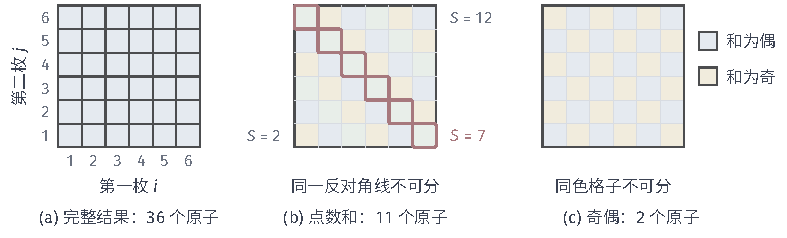
\includegraphics[width=133mm]{figures/02-abstract-mathematics/02-probability-spaces/tikz/pmod-dice-information/figure.pdf}
  \caption{两枚公平骰子的三种记录。格子$(i,j)$表示第一枚$i$点、第二枚$j$点，$36$格等可能。(a) 完整记录，每格单独可辨；(b) 只记录点数和$S$，同一条反对角线上的格子同色、不可区分，共$11$块（图中称原子），红框为$\{S=7\}$；(c) 只记录$S$的奇偶，只剩两块。颜色只区分相邻的块，不表示概率大小。}
  \label{fig:pmod-dice-information}
\end{figure*}

\paragraph{不必有密度的概率测度}
卷一的概率模型大多由概率表或普通密度给出。
在实轴的Borel结构上，这两类分别是点质量的可数混合$\sum_kp_k\delta_{x_k}$，以及形如$A\mapsto\int_Af(x)\,dx$的测度。
第~\ref{sec:measure-same-space-comparison}节的Lebesgue分解说明，实轴上的任何概率测度都可以写成相对长度绝对连续的部分与奇异部分之和；奇异部分可以含点质量，也可以不含任何点质量。

后一种情况的典型例子是\term{Cantor分布}（Cantor distribution）。
把三进制展开中每一位独立、等可能地取$0$或$2$，得到$[0,1]$中的随机点（这样的独立数字可以在$[0,1)$均匀模型上实现，见第~\ref{sec:pmod-independence}节的例~\ref{ex:pmod-binary-digits}）。
前$n$位数字的$2^n$种取法对应$2^n$个互不相交、长度为$3^{-n}$的闭区间，随机点落在哪个区间由前$n$位数字决定，概率为$2^{-n}$。任一单点至多属于其中一个区间，所以它的概率不超过$2^{-n}$；这对一切$n$成立，因而为零。
同时全部质量落在$2^n$个这样的区间之并中，总长度$(2/3)^n\to0$。
这个分布既没有概率表，也没有相对长度的密度。
章首的等待时间则是点质量与密度部分的混合。
本部分直接以测度$\mathbb P$为对象作计算，不要求它属于某种表示；常见分布族的系统整理放在\BookPartRef{part:probability-distributions}{卷四“概率分布”部分}。

\subsection{零概率事件与几乎必然}

\paragraph{零概率不等于不可能}
在$[0,1]$上取Borel$\sigma$代数与长度，得到\emph{$[0,1]$均匀模型}；令$X(\omega)=\omega$。
对任意固定的$x\in[0,1]$和$h>0$，事件$\{X=x\}$包含于$\{x-h\le X\le x+h\}$，后者的概率不超过$2h$。
令$h\to0$，得$\mathbb P(X=x)=0$。
可是$\{X=x\}=\{x\}$并不是空集：结果恰好是$x$完全可能发生，每次试验中$X$也总要取到$[0,1]$中的某个值。这个非空事件的概率却为零。

概率为零的事件称为\term{零概率事件}（null event），它必须和空事件分开。
空事件在任何概率测度下都不发生；零概率事件可以发生，只是在模型的累计意义下不占质量。
零概率也总是相对于具体的$\mathbb P$而言：在点质量$\delta_x$下，单点$\{x\}$的概率是$1$。

\paragraph{几乎必然的定义}
很多结论在个别结果上失败，但失败的结果合起来没有概率。
第~\ref{chap:measure-spaces}章称这样的性质“几乎处处”成立；在概率空间上习惯说“几乎必然”。

\begin{definition}[几乎必然]
\label{def:pmod-almost-sure}
设$(\Omega,\mathcal F,\mathbb P)$是概率空间，$\mathcal Q$是关于样本点$\omega$的一个命题。
若存在事件$N\in\mathcal F$，$\mathbb P(N)=0$，使得每个$\omega\notin N$都满足$\mathcal Q$，就称$\mathcal Q$\term{几乎必然}（almost surely）成立，简记为a.s.。
等价地，存在概率为$1$的事件，在其上$\mathcal Q$处处成立。
\end{definition}

定义只要求失败的结果被某个零概率事件盖住，不要求失败集合本身是事件。
这一区别在下文讨论完备化时会用到。

\begin{example}[只在一点失败的极限]
\label{ex:pmod-power-limit}
在$[0,1]$均匀模型上令$X_n(\omega)=\omega^n$。
当$0\le\omega<1$时$\omega^n\to0$；当$\omega=1$时$X_n(1)=1$对一切$n$成立。
取$N=\{1\}$，$\mathbb P(N)=0$，在$N$之外$X_n\to0$，所以$X_n\to0$几乎必然成立。
它不是处处成立的：在$\omega=1$这个结果上，极限是$1$。
\end{example}

图~\ref{fig:pmod-almost-sure-limit}画出了几条$\omega\mapsto\omega^n$。
$n$越大，曲线越早贴近$0$，只在右端急剧抬升到$1$；逐点极限是除右端点外恒为零的函数。
抬升的区域越来越窄，但对每个固定的$n$都存在；真正的例外只剩一点，它不占概率。

\begin{figure}[htbp]
  \centering
  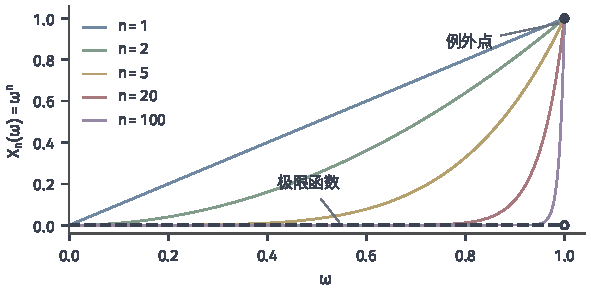
\includegraphics[width=100mm]{figures/02-abstract-mathematics/02-probability-spaces/matplotlib/pmod-almost-sure-limit/figure.pdf}
  \caption{$[0,1]$均匀模型上的$X_n(\omega)=\omega^n$，$n=1,2,5,20,100$。虚线是逐点极限：$\omega<1$时为$0$，$\omega=1$时为$1$（实心点）。例外集合$\{1\}$的概率为零，所以$X_n\to0$几乎必然成立，但不是处处成立。}
  \label{fig:pmod-almost-sure-limit}
\end{figure}

\paragraph{例外集合的合并与量词}
设一列命题$\mathcal Q_1,\mathcal Q_2,\dots$各自几乎必然成立，例外分别被零概率事件$N_1,N_2,\dots$盖住。
取$N=\bigcup_kN_k$，由可数次可加性
\[
  \mathbb P(N)\le\sum_{k=1}^\infty\mathbb P(N_k)=0,
\]
而在$N$之外所有$\mathcal Q_k$同时成立。
所以“对每个$k$几乎必然成立”可以升级为“几乎必然对所有$k$同时成立”：可数多个例外可以并入一个共同的零概率事件。

不可数多个例外没有这个保证。
在$[0,1]$均匀模型中，对每个固定的$x$，“$X\ne x$”几乎必然成立，因为例外集合$\{x\}$的概率为零。
但“对所有$x\in[0,1]$都有$X\ne x$”在任何结果上都不成立：所有单点的并就是整个$\Omega$。
因此遇到“对所有$t$”这类量词时，先数清$t$的范围：可数时直接合并例外；不可数时需要连续性或可分性等额外结构，把问题化为可数个时刻。
后面讨论随机变量列的收敛时，指标$n$只取可数个值，这正是可以直接合并例外的情形。

\paragraph{零概率集合上的改动}
“几乎必然”允许我们在零概率集合上忽略差异，但改动一个随机变量时还要核对可测性。
设$N\in\mathcal F$，$\mathbb P(N)=0$，$S\subseteq N$，把可测函数$X$在$S$上改成别的值得到$Y$。
若$S$本身不在$\mathcal F$中，$\{Y\in B\}$可能包含$S$的某个不可测部分，于是$Y$不一定可测。

有两种处理方式。
一是改用完备化的概率空间$(\Omega,\overline{\mathcal F},\overline{\mathbb P})$：把零概率事件的全部子集补进事件范围，原有事件的概率不变，此时零概率集合上的任意改动都保持可测（完备化的构造见第~\ref{sec:measure-general-structure}节）。
二是只在可测的零概率事件上、以可测的方式改动，例如把$X$在$N$上改成$0$。
本部分说两个随机变量“几乎必然相等”时，两者都假定是可测的；所谓选取一个“版本”，指在几乎必然相等的可测函数中选一个代表，所有概率与期望都不依赖这一选择。

\section{随机对象与观测信息}
\label{sec:pmod-random-objects}

固定概率空间之后，我们关心的通常不是$\omega$本身，而是对它的某种观测：骰子点数和、等待时长、一个特征向量或一张网络。
本节先说明一个观测需要满足什么条件，才能对“观测值落在某处”谈概率；再说明一个观测让我们能分辨哪些事件。

\subsection{随机对象的可测性}

\paragraph{可测映射与可问的事件}
设观测把每个结果$\omega$送到某个取值空间中的点$X(\omega)$。
我们想问的是$\mathbb P(X\in B)$，即结果集合
\[
  \{X\in B\}=\{\omega\in\Omega:X(\omega)\in B\}=X^{-1}(B)
\]
的概率。
这要求$X^{-1}(B)$属于$\mathcal F$，否则概率根本没有定义。
取值空间同样要先规定哪些集合$B$可以问，于是它也是一个可测空间。

\begin{definition}[随机对象]
\label{def:pmod-random-object}
设$(\Omega,\mathcal F,\mathbb P)$是概率空间，$(E,\mathcal E)$是可测空间。
若映射$X:\Omega\to E$对每个$B\in\mathcal E$都满足$X^{-1}(B)\in\mathcal F$，就称$X$是取值于$(E,\mathcal E)$的\term{随机对象}（random element）。
取值于$(\mathbb R,\mathcal B(\mathbb R))$的随机对象称为\term{随机变量}（random variable），取值于$(\mathbb R^d,\mathcal B(\mathbb R^d))$的称为$d$维\term{随机向量}（random vector）。
\end{definition}

换句话说，随机对象就是从$(\Omega,\mathcal F)$到$(E,\mathcal E)$的可测映射，“随机”只来自$\omega$的不确定，映射本身是确定的。
图~\ref{fig:pmod-preimage}画出了这一关系：取值空间中的集合$B$被拉回为样本空间中的事件$\{X\in B\}$，后者可以由不相连的几块组成，只要它属于$\mathcal F$就有概率。
注意记号$X^{-1}(B)$只表示原像，并不要求$X$可逆。

\begin{figure*}[htbp]
  \centering
  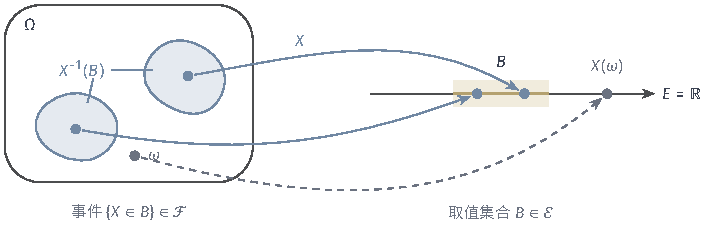
\includegraphics[width=120mm]{figures/02-abstract-mathematics/02-probability-spaces/tikz/pmod-preimage/figure.pdf}
  \caption{随机对象$X$是从样本空间$\Omega$到取值空间$E$的映射。取值集合$B$（右侧黄色区间）的原像$X^{-1}(B)=\{X\in B\}$是$\Omega$中的蓝色区域，可以分成不相连的几块；落在区域外的$\omega$被送到$B$之外。可测性要求每个$B\in\mathcal E$的原像都是事件。示意图，不含数值。}
  \label{fig:pmod-preimage}
\end{figure*}

\paragraph{常见的取值空间}
取值空间的可测结构要按问题选定，然后才能核对“哪些问题是事件”。
实值观测用实轴的Borel结构，有限维向量用$\mathbb R^d$的Borel结构；由第~\ref{chap:measure-spaces}章，$\mathcal B(\mathbb R^d)$与$d$个$\mathcal B(\mathbb R)$的乘积$\sigma$代数相同。
$m\times n$的\term{随机矩阵}（random matrix）把$\mathbb R^{m\times n}$按元素等同于$\mathbb R^{mn}$，沿用其Borel结构。
需要允许$\pm\infty$时（例如一列随机变量的上确界），取扩充实轴$[-\infty,+\infty]$，其可测集是形如$B\cup D$的集合，其中$B\in\mathcal B(\mathbb R)$，$D\subseteq\{-\infty,+\infty\}$。

离散的结构对象也可以作为取值空间。
固定顶点集$V=\{1,\dots,n\}$，所有简单无向图组成有限集$\mathcal G_n$，共有$2^{n(n-1)/2}$个元素，取其幂集为可测结构。
一个随机简单图$G:\Omega\to\mathcal G_n$可测，当且仅当每个$\{G=g\}$都是事件；这又等价于每条边的指示$\mathbb I_{\{\{i,j\}\in G\}}$都是随机变量。
前一个方向成立，是因为“边$\{i,j\}$出现”是有限个$\{G=g\}$的并；后一个方向成立，是因为$\{G=g\}$是有限个“某边出现”或“某边不出现”的交。
由于$\mathcal G_n$的每个子集都可测，“$G$连通”“$G$含三角形”这类问题在$G$可测时自动是事件。

\paragraph{用生成族检查可测性}
逐个检查$\mathcal E$中所有集合的原像通常做不到，好在取原像与补集、可数并可以交换。
若$\mathcal E$由集合族$\mathcal C$生成，则满足$X^{-1}(B)\in\mathcal F$的$B$构成一个$\sigma$代数，只要它包含$\mathcal C$就包含整个$\mathcal E$。
于是对实值$X$，只需检查$\{X\le a\}\in\mathcal F$对每个实数$a$（甚至每个有理数$a$）成立。

对$\bm X=(X_1,\dots,X_d)$，$\bm X$是随机向量当且仅当每个坐标$X_i$都是随机变量。
若$\bm X$可测，坐标投影连续因而Borel可测，$X_i$是可测映射的复合，仍可测；反过来，若每个$X_i$可测，则
\[
  \{\bm X\in(-\infty,a_1]\times\cdots\times(-\infty,a_d]\}=\bigcap_{i=1}^d\{X_i\le a_i\}\in\mathcal F,
\]
而这类左下象限生成$\mathcal B(\mathbb R^d)$。
复合保持可测：若$g:(E,\mathcal E)\to(E',\mathcal E')$可测，则$(g\circ X)^{-1}(C)=X^{-1}(g^{-1}(C))$，所以$g(X)$也是随机对象。
据此，$X+Y$、$XY$、$\max\{X,Y\}$、$|X|^p$都是随机变量，因为它们是随机向量$(X,Y)$的连续函数；一列随机变量的$\sup_n$、$\liminf_n$、$\limsup_n$是扩充实值随机变量，因为它们只涉及可数次运算。

可测性只保证所问的事件有概率，不提供更多性质。
它不意味着$X$关于$\omega$连续（$\Omega$上甚至可以没有拓扑），不意味着$X$与其他观测独立，也不意味着$X$的期望有限。
取值为整条曲线或整个函数时，选择什么可测结构取决于要问哪些问题，这在第~\ref{part:function-spaces}部分和\BookPartRef{part:dynamical-systems-control-decision-and-games}{卷三“过程与轨迹演化”部分}按用途建立，本章只处理有限维与一般可测取值对象的共同结构。

\subsection{随机对象生成的信息}

\paragraph{观测能分辨哪些事件}
只看到骰子点数和$S$的记录员，能判断的恰好是形如$\{S\in B\}$的事件：知道$S(\omega)$以后，就知道$\omega$是否落在其中。
一般观测也是如此。

\begin{definition}[随机对象生成的$\sigma$代数]
\label{def:pmod-generated-sigma}
设$X$是取值于$(E,\mathcal E)$的随机对象。称
\[
  \sigma(X)=\{X^{-1}(B):B\in\mathcal E\}
\]
为$X$生成的$\sigma$代数。
\end{definition}

由于取原像与补集、可数并交换，$\sigma(X)$确实是$\sigma$代数；由$X$的可测性，$\sigma(X)\subseteq\mathcal F$。
任何使$X$可测的$\sigma$代数$\mathcal G$都必须包含全部$X^{-1}(B)$，所以$\sigma(X)$是$\Omega$上使$X$可测的最小$\sigma$代数。
它的含义是：一个事件$A$属于$\sigma(X)$，当且仅当它可以写成$\{X\in B\}$的形式，于是知道$X(\omega)$就能判断$\omega$是否属于$A$。
在例~\ref{ex:pmod-dice-records}中，$\sigma(S)=\mathcal F_{\mathrm{sum}}$，而奇偶记录生成的正是$\mathcal F_{\mathrm{par}}$。

\paragraph{变换只会减少信息}
对观测作进一步加工，只能丢掉信息，不能凭空增加。
设$g:(E,\mathcal E)\to(E',\mathcal E')$可测，$Y=g(X)$。对每个$C\in\mathcal E'$，
\[
  Y^{-1}(C)=X^{-1}\bigl(g^{-1}(C)\bigr)\in\sigma(X),
\]
所以
\begin{equation}
  \sigma(g(X))\subseteq\sigma(X).
  \label{eq:pmod-function-information}
\end{equation}
信息减少因此有了精确的意思：$g(X)$能判断的事件是$X$能判断的事件的一部分。
若$g$是双射且逆映射也可测，上式两边相等，可逆的重新编码不改变信息。

\begin{example}[区间上的两级观测]
\label{ex:pmod-interval-information}
在$[0,1)$上取Borel$\sigma$代数与长度，令$X(\omega)=\lfloor4\omega\rfloor$，$Y=\lfloor X/2\rfloor=\lfloor2\omega\rfloor$。
$X$取$0,1,2,3$，把$\Omega$分成四个长$1/4$的区间；$\sigma(X)$由这些区间的并组成，共$2^4=16$个事件。
$Y$只取$0,1$，$\sigma(Y)=\{\varnothing,[0,1/2),[1/2,1),\Omega\}$。
事件$\{X=1\}=[1/4,1/2)$属于$\sigma(X)$，却只是$\{Y=0\}$的一半，所以不属于$\sigma(Y)$：知道$Y=0$并不能判断$X$是否为$1$。
\end{example}

图~\ref{fig:pmod-generated-partitions}把两级观测上下对齐（图中把不可再分的块称为原子）。
上一行的每个块都完整地落在下一行的某个块里，这就是式~\eqref{eq:pmod-function-information}的图形含义；反过来，下一行的块不能拆开，红框中的事件对$Y$不可见。
对取有限个值的观测（取值空间中单点可测），$\sigma(X)$总是由它的等值块的并组成，信息的多少就是划分的粗细。
反过来的问题——若$\sigma(Y)\subseteq\sigma(X)$，$Y$是否一定是$X$的函数——由第~\ref{chap:conditional-expectation}章的Doob--Dynkin引理（定理~\ref{thm:cond-doob-dynkin}）给出肯定回答。

\begin{figure*}[htbp]
  \centering
  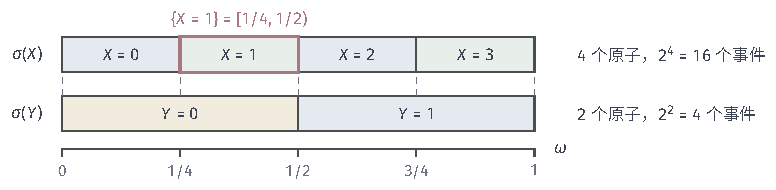
\includegraphics[width=131mm]{figures/02-abstract-mathematics/02-probability-spaces/tikz/pmod-generated-partitions/figure.pdf}
  \caption{$[0,1)$均匀模型上的两级观测。上行$X=\lfloor4\omega\rfloor$把区间分成四块，生成$16$个事件；下行$Y=\lfloor X/2\rfloor$只分成两块，生成$4$个事件。虚线表明$X$的每一块都落在$Y$的某一块内；红框中的$\{X=1\}$属于$\sigma(X)$而不属于$\sigma(Y)$。}
  \label{fig:pmod-generated-partitions}
\end{figure*}

\paragraph{多个观测的共同信息}
同时看到有限个观测$X_1,\dots,X_m$时，把它们合成一个映射$(X_1,\dots,X_m)$，取值于乘积空间$E_1\times\cdots\times E_m$，其可测结构为乘积$\sigma$代数$\mathcal E_1\otimes\cdots\otimes\mathcal E_m$。
矩形的原像是
\[
  \{(X_1,\dots,X_m)\in B_1\times\cdots\times B_m\}=\bigcap_{i=1}^m\{X_i\in B_i\},
\]
它属于$\mathcal F$；矩形生成乘积$\sigma$代数，所以合成映射可测。
记$\sigma(X_1,\dots,X_m)=\sigma\bigl((X_1,\dots,X_m)\bigr)$。

这个$\sigma$代数恰好是包含$\sigma(X_1)\cup\cdots\cup\sigma(X_m)$的最小$\sigma$代数，也就是“把各个观测的信息合起来”。一方面，$X_i$是合成映射与坐标投影的复合，所以每个$\sigma(X_i)$都含于$\sigma(X_1,\dots,X_m)$；另一方面，记$\mathcal G$为包含这些$\sigma(X_i)$的最小$\sigma$代数，原像属于$\mathcal G$的乘积可测集构成一个$\sigma$代数，它包含全部矩形，因而就是整个乘积$\sigma$代数，于是$\sigma(X_1,\dots,X_m)\subseteq\mathcal G$。

“分别观察”与“联合观察”在这里有确切的区别。
对两枚骰子，记第一枚点数为$D_1$，第二枚为$D_2$。
事件$\{S=7\}$既不属于$\sigma(D_1)$，也不属于$\sigma(D_2)$，因而不属于两者之并；但它属于$\sigma(D_1,D_2)$，因为把两个数加起来需要同时知道两枚的点数。
两个$\sigma$代数之并一般不再是$\sigma$代数，联合观察得到的是由它生成的更大的集合族。

有了$\sigma(X_1,\dots,X_m)$，就可以精确地说“已知这些观测”指什么。
已知部分信息后怎样重新求平均、怎样写出其余量的条件分布，是第~\ref{chap:conditional-expectation}章的问题；本章只把信息本身写清楚，不提前使用条件期望，也不引入随时间增长的信息族。

\section{随机对象的分布}
\label{sec:pmod-distributions}

上一节的问题都发生在样本空间里：哪个$\omega$被送到哪里，哪些事件可以判断。
实际计算时，我们往往只关心观测值落在各处的概率，而不关心是哪些$\omega$把它送过去的。
本节把概率搬到取值空间，得到分布；再比较只看分布时会丢掉什么，以及多个观测一起看时需要什么新信息。

\subsection{分布与推前测度}

\paragraph{分布是取值空间上的概率测度}
对取值于$(E,\mathcal E)$的随机对象$X$，每个$B\in\mathcal E$都有概率$\mathbb P(X\in B)$。
把它看成$B$的函数，就是第~\ref{sec:measure-cross-space}节的推前测度。

\begin{definition}[分布]
\label{def:pmod-distribution}
设$X$是概率空间$(\Omega,\mathcal F,\mathbb P)$上取值于$(E,\mathcal E)$的随机对象。$(E,\mathcal E)$上的概率测度
\[
  P_X(B)=\mathbb P(X\in B)=\mathbb P\bigl(X^{-1}(B)\bigr),\qquad B\in\mathcal E,
\]
即推前测度$X_\#\mathbb P$，称为$X$的\term{分布}（distribution）或概率分布。
\end{definition}

推前保持总质量与可数可加性，所以$P_X$确实是$(E,\mathcal E)$上的概率测度。
分布回答“观测值落在$B$中的概率多大”，它住在取值空间，与样本空间的具体形状无关。

\begin{example}[把均匀质量搬成指数分布]
\label{ex:pmod-exponential-pushforward}
在$[0,1)$均匀模型上令$X(\omega)=-\ln(1-\omega)$。
取$B=[1,2]$，由于$X$严格递增，
\[
  \{X\in B\}=\bigl[1-e^{-1},\,1-e^{-2}\bigr],\qquad
  \mathbb P(X\in B)=e^{-1}-e^{-2}\approx0.233.
\]
一般地，对$x\ge0$有$\mathbb P(X\le x)=\mathbb P(\omega\le1-e^{-x})=1-e^{-x}$，所以$P_X$是率参数为$1$的指数分布。
\end{example}

图~\ref{fig:pmod-pushforward-exponential}把这个例子拆成两步。
左图在样本空间上：黄色横带是取值集合$B$，蓝色竖带是它的原像，竖带的长度就是概率。
右图在取值空间上：同一个概率表现为密度曲线下的黄色面积。
左边的均匀质量被映射$X$拉伸后重新分布，靠近$\omega=1$的一小段被拉成很长的尾部，所以右边的密度递减。
这也是用均匀随机数生成指数随机数的依据。

\begin{figure*}[htbp]
  \centering
  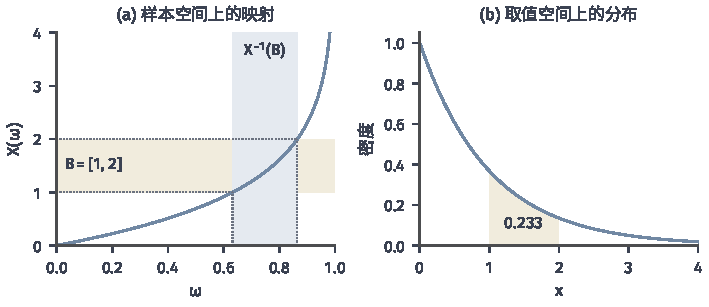
\includegraphics[width=120mm]{figures/02-abstract-mathematics/02-probability-spaces/matplotlib/pmod-pushforward-exponential/figure.pdf}
  \caption{推前测度的两种读法。$[0,1)$均匀模型上$X(\omega)=-\ln(1-\omega)$，$B=[1,2]$。(a) 样本空间上，$B$（黄色横带）的原像是区间$[1-e^{-1},1-e^{-2}]$（蓝色竖带），长度约$0.233$；(b) 取值空间上，$P_X$为指数分布，$B$上的密度面积同为$e^{-1}-e^{-2}\approx0.233$。}
  \label{fig:pmod-pushforward-exponential}
\end{figure*}

\paragraph{概率表、密度与分布函数}
卷一计算分布时用的三种工具，都是$P_X$的不同表示。
离散随机变量的概率表$p(x)=\mathbb P(X=x)$给出$P_X=\sum_xp(x)\delta_x$；有密度$f$的随机变量满足$P_X(B)=\int_Bf(x)\,dx$，这正是说$P_X$相对长度绝对连续，$f$是它的相对密度。
第三种工具是\term{分布函数}（distribution function）$F_X(x)=\mathbb P(X\le x)$，它对任何实值随机变量都存在。

分布函数完全确定分布。
半直线族$\{(-\infty,a]:a\in\mathbb R\}$加上$\mathbb R$本身，对有限交封闭并生成$\mathcal B(\mathbb R)$；两个概率测度若在这些集合上取值相同，由定理~\ref{thm:measure-pi-lambda-uniqueness}，它们在整个$\mathcal B(\mathbb R)$上相同。
所以$F_X=F_Y$当且仅当$P_X=P_Y$。
这解释了卷一的做法：先求分布函数，再求导得到密度，背后识别的始终是同一个测度$P_X$；分布函数在概率表与密度都不存在时仍然可用，例如章首的等待时间和Cantor分布。
这些基本计算的具体做法可参考\BookChapterRef{chap:random-variables}{卷一“随机变量与概率分布”章}。

\paragraph{变换后的分布}
对可测映射$g$，$g(X)$的分布由原像直接确定：
\[
  P_{g(X)}(C)=\mathbb P\bigl(X\in g^{-1}(C)\bigr)=P_X\bigl(g^{-1}(C)\bigr),
  \qquad\text{即}\qquad P_{g(X)}=g_\#P_X.
\]
求变换后的分布时，应先写出事件的原像，再看是否能用密度换元公式化简。
取$X$服从$[0,1]$上的均匀分布，$Y=X^2$。对$0\le y\le1$，
\[
  \mathbb P(Y\le y)=\mathbb P\bigl(X\le\sqrt y\bigr)=\sqrt y,
\]
求导得$Y$在$(0,1)$上的密度$1/(2\sqrt y)$，与第~\ref{sec:measure-cross-space}节的换元公式（取$(0,1)$上的光滑可逆映射$x\mapsto x^2$）一致。
若$g(x)=\mathbb I_{\{x>1/2\}}$，换元公式无从使用，因为$Y=g(X)$只取$0,1$，没有密度；原像方法照样给出$\mathbb P(Y=1)=\mathbb P(X>1/2)=1/2$。

随机对象$X$与它的分布$P_X$是不同类型的对象。
$X$是$\Omega$上的映射，记录每个结果对应哪个取值；$P_X$是$E$上的测度，只记录各取值集合上一共有多少概率。
从$X$可以算出$P_X$，从$P_X$却不能恢复$X$：许多不同的映射会推出同一个测度。
下一小节专门讨论这一差别。

\subsection{同分布与几乎处处相等}

\paragraph{三种相等关系}
说两个随机量“相同”，可以有三种不同强度的含义。

\begin{definition}[同分布]
\label{def:pmod-identical-distribution}
设$X$与$Y$取值于同一个可测空间$(E,\mathcal E)$，它们可以定义在不同的概率空间上。若$P_X=P_Y$，称$X$与$Y$\term{同分布}（identically distributed），记为$X\overset{d}{=}Y$。
\end{definition}

另外两种相等都要求$X,Y$定义在同一个概率空间上。
\emph{处处相等}指$X(\omega)=Y(\omega)$对每个$\omega$成立；\emph{几乎处处相等}（也说几乎必然相等）指它们在某个零概率事件之外相等，记为$X=Y$ a.s.。
对实值或有限维随机向量，$\{X\ne Y\}$本身是事件，几乎处处相等就是$\mathbb P(X\ne Y)=0$。

三者之间有单向的蕴含：处处相等蕴含几乎处处相等，几乎处处相等蕴含同分布。
后一步是因为对每个$B$，$\{X\in B\}$与$\{Y\in B\}$只在$\{X\ne Y\}$上可能不同，
\[
  \bigl|\mathbb P(X\in B)-\mathbb P(Y\in B)\bigr|\le\mathbb P(X\ne Y)=0.
\]
前两种相等比较的是同一个样本点上的取值，所以必须有共同的概率空间；同分布只比较取值空间上的两个测度，可以跨越不同的试验。
例如今天掷的公平硬币与明天掷的公平硬币同分布，但问“两枚硬币是否几乎处处相等”，要先把两次试验放进同一个概率空间才有意义。

\paragraph{同分布而不相等}
同分布推不出几乎处处相等，最简单的例子来自一次翻转。

\begin{example}[均匀变量与它的翻转]
\label{ex:pmod-reflection-uniform}
在$[0,1]$均匀模型上令$X(\omega)=\omega$，$Y(\omega)=1-\omega$。
对$0\le x\le1$，$\mathbb P(Y\le x)=\mathbb P(\omega\ge1-x)=x=\mathbb P(X\le x)$，所以$X\overset{d}{=}Y$，两者都服从$[0,1]$上的均匀分布。
但$X(\omega)=Y(\omega)$只在$\omega=1/2$时成立，$\mathbb P(X=Y)=0$；平均距离$\mathbb E|X-Y|=\int_0^1|2\omega-1|\,d\omega=1/2$。
\end{example}

图~\ref{fig:pmod-reflection-uniform}左图在样本空间上比较两者：对同一个$\omega$，两条直线给出不同的值，竖线标出$\omega=1/4$处的差距$1/2$。
右图在取值空间上比较两者：两条分布函数完全重合。
分布只看右图，所以无法区分$X$与$Y$；任何只依赖分布的量，例如$\mathbb P(X>0.9)$或$\mathbb E X^2$，两者都相同。

\begin{figure}[htbp]
  \centering
  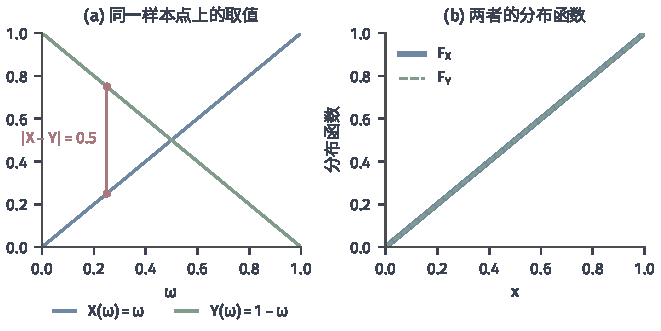
\includegraphics[width=112mm]{figures/02-abstract-mathematics/02-probability-spaces/matplotlib/pmod-reflection-uniform/figure.pdf}
  \caption{$[0,1]$均匀模型上的$X(\omega)=\omega$与$Y(\omega)=1-\omega$。(a) 同一样本点上的取值，竖线标出$\omega=1/4$处$|X-Y|=1/2$，两者只在$\omega=1/2$处相等；(b) 两者的分布函数都是$F(x)=x$，图中完全重合。}
  \label{fig:pmod-reflection-uniform}
\end{figure}

\paragraph{相同边缘下的不同轨迹}
同样的现象出现在随机变量列中，而且影响更大：各项的分布相同，不能决定整列在样本点上的行为。

\begin{example}[常值比特列与交替比特列]
\label{ex:pmod-alternating-bits}
设$Z\sim\operatorname{Bernoulli}(1/2)$，例如在$[0,1)$均匀模型上取$Z=\mathbb I_{\{\omega\ge1/2\}}$。
令$X_n=Z$对一切$n$成立，并令
\[
  Y_n=\begin{cases}Z,&n\text{为奇数},\\1-Z,&n\text{为偶数}.\end{cases}
\]
由于$1-Z$也服从$\operatorname{Bernoulli}(1/2)$，每个$X_n$与每个$Y_n$都服从$\operatorname{Bernoulli}(1/2)$，两列的各项分布完全相同。
但$X_n(\omega)$对每个$\omega$都是常数列，处处收敛；$Y_n(\omega)$对每个$\omega$都在$0$与$1$之间交替，处处不收敛。
两列的差别在多项之间的联合规律上：$\mathbb P(X_1=X_2)=1$，而$\mathbb P(Y_1=Y_2)=0$。
\end{example}

图~\ref{fig:pmod-alternating-paths}分别画出$Z=0$与$Z=1$时两列的取值。
圆点构成的$X_n$是水平线；方块构成的$Y_n$锯齿式跳动，对两种$Z$都是如此。
如果只记录“第$n$项服从什么分布”，这两张图给不出任何区别。
因此第~\ref{chap:random-variable-convergence}章研究随机变量列在同一样本点上的收敛时，必须使用共同的概率空间；而第~\ref{chap:weak-convergence-limit-theorems}章只比较分布时，这两列都平凡地“分布收敛”到$\operatorname{Bernoulli}(1/2)$，样本点上的差别被完全忽略。

\begin{figure}[htbp]
  \centering
  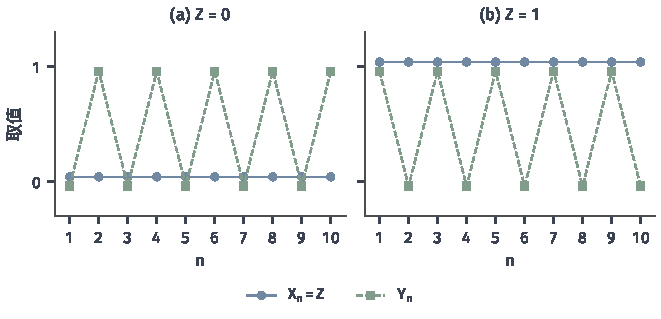
\includegraphics[width=112mm]{figures/02-abstract-mathematics/02-probability-spaces/matplotlib/pmod-alternating-paths/figure.pdf}
  \caption{同一公平比特$Z$构造的两列随机变量，横轴为下标$n=1,\dots,10$。圆点为$X_n=Z$，方块为在$Z$与$1-Z$之间交替的$Y_n$。(a) $Z=0$；(b) $Z=1$。为避免重合，两列在竖直方向各错开$0.04$。两列每一项都服从$\operatorname{Bernoulli}(1/2)$，但前者处处收敛，后者处处不收敛。}
  \label{fig:pmod-alternating-paths}
\end{figure}

\subsection{联合分布与边缘分布}

\paragraph{联合分布的定义}
例~\ref{ex:pmod-alternating-bits}说明，比较多个随机对象时需要它们一起出现的规律。
上一节已经把有限个随机对象合成为乘积空间中的一个可测映射，它的分布就是这种规律。

\begin{definition}[联合分布与边缘分布]
\label{def:pmod-joint-distribution}
设$X_1,\dots,X_m$定义在同一个概率空间上，$X_i$取值于$(E_i,\mathcal E_i)$。
随机对象$(X_1,\dots,X_m)$在$(E_1\times\cdots\times E_m,\ \mathcal E_1\otimes\cdots\otimes\mathcal E_m)$上的分布
\[
  P_{(X_1,\dots,X_m)}(C)=\mathbb P\bigl((X_1,\dots,X_m)\in C\bigr)
\]
称为$X_1,\dots,X_m$的\term{联合分布}（joint distribution）；相对于它，每个$P_{X_i}$称为\term{边缘分布}（marginal distribution）。
\end{definition}

边缘分布由联合分布唯一确定。
记坐标投影$\pi_i(x_1,\dots,x_m)=x_i$，则$X_i=\pi_i\circ(X_1,\dots,X_m)$，由推前的复合规则，
\[
  P_{X_i}=(\pi_i)_\#P_{(X_1,\dots,X_m)},\qquad
  P_{X_i}(B)=P_{(X_1,\dots,X_m)}\bigl(E_1\times\cdots\times B\times\cdots\times E_m\bigr).
\]
在概率表中，这就是按行或按列求和；在密度模型中，这就是对其余坐标积分。
这里不要求联合分布有密度，也不要求$E_i$是实轴：定义只用到乘积可测结构与推前。

\paragraph{边缘不能决定联合}
反过来，各个边缘一般不能恢复联合分布。
具有给定边缘的联合分布称为这些边缘的一个\term{耦合}（coupling）；同一组边缘通常有许多耦合。

\begin{example}[相同边缘的三种配对]
\label{ex:pmod-bernoulli-couplings}
在$[0,1)$均匀模型上令$X=\mathbb I_{\{\omega\ge1/2\}}$，并考虑三种$Y$：
\[
  Y^{(a)}=X,\qquad Y^{(b)}=1-X,\qquad
  Y^{(c)}=\mathbb I_{\{\omega\in[1/4,1/2)\cup[3/4,1)\}}.
\]
三个$Y$都服从$\operatorname{Bernoulli}(1/2)$，与$X$的边缘也相同。
三种联合概率表依次为：同向配对把概率$1/2,1/2$放在对角格$(0,0),(1,1)$上；反向配对放在反对角格$(0,1),(1,0)$上；第三种配对中，例如$\mathbb P(X=1,Y^{(c)}=1)=\mathbb P([3/4,1))=1/4$，四格都是$1/4$。
于是$\mathbb P(X=Y)$依次为$1,0,1/2$，$\mathbb P(X+Y=2)$依次为$1/2,0,1/4$，协方差依次为$1/4,-1/4,0$。
\end{example}

图~\ref{fig:pmod-bernoulli-couplings}列出了三张表。
三张表的行和、列和完全相同，都是$(1/2,1/2)$，差别只在四个格子之间如何分配概率。
所以边缘分布缺少的不是某个单独对象的参数，而是“哪些取值同时出现”的规律；任何同时涉及$X$与$Y$的量，例如$X+Y$的分布、$\mathbb P(X=Y)$或协方差，都要由联合分布决定。
第三种配对的四格恰好等于边缘之积，下一节会看到这正是独立的情形。
在给定边缘的众多耦合中如何比较与挑选，属于卷四“概率分布”部分的问题。

\begin{figure*}[htbp]
  \centering
  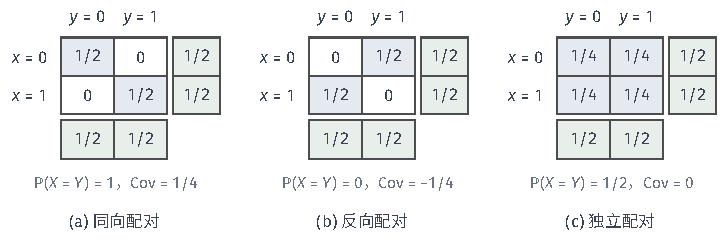
\includegraphics[width=122mm]{figures/02-abstract-mathematics/02-probability-spaces/tikz/pmod-bernoulli-couplings/figure.pdf}
  \caption{两个$\operatorname{Bernoulli}(1/2)$变量的三种联合概率表。行为$X$的取值，列为$Y$的取值，绿色格为边缘概率，蓝色格为取正概率的组合。(a) 同向配对$Y=X$；(b) 反向配对$Y=1-X$；(c) 独立配对，四格都等于边缘之积。三表的边缘完全相同，$\mathbb P(X=Y)$与协方差却不同。}
  \label{fig:pmod-bernoulli-couplings}
\end{figure*}

\section{独立性}
\label{sec:pmod-independence}

联合分布写清了多个观测一起出现的规律。
在例~\ref{ex:pmod-bernoulli-couplings}的三种配对中，只有第三种的联合概率表恰好等于边缘之积：知道$X$的取值，对$Y$落在哪里没有任何影响。
本节把这种“没有概率依赖”的关系推广到一般随机对象，证明它等价于联合分布分解为乘积测度，并说明它在变换与分组之后如何保留。

\subsection{事件族与随机对象的独立性}

\paragraph{从事件的乘法判据到$\sigma$代数}
卷一称事件$A_1,\dots,A_n$相互独立，是指其中任意一部分事件之交的概率等于各自概率之积。
这个条件也自动覆盖了补事件：例如由$\mathbb P(A\cap B)=\mathbb P(A)\mathbb P(B)$可得
\[
  \mathbb P\bigl((\Omega\setminus A)\cap B\bigr)=\mathbb P(B)-\mathbb P(A\cap B)=\mathbb P(\Omega\setminus A)\,\mathbb P(B).
\]
所以一个事件$A$的独立性，实际上是它生成的整个$\sigma$代数$\{\varnothing,A,\Omega\setminus A,\Omega\}$的独立性。
对随机对象，我们关心的是它能判断的全部事件，即$\sigma(X)$；这提示我们直接对$\sigma$代数定义独立。

\begin{definition}[$\sigma$代数与随机对象的独立性]
\label{def:pmod-independence}
设$(\Omega,\mathcal F,\mathbb P)$是概率空间，$(\mathcal G_i)_{i\in I}$是一族子$\sigma$代数，$\mathcal G_i\subseteq\mathcal F$，指标集$I$可以有限、可数或更大。
若对每个有限非空子集$J\subseteq I$及任意选取的$A_j\in\mathcal G_j$（$j\in J$），都有
\[
  \mathbb P\Bigl(\bigcap_{j\in J}A_j\Bigr)=\prod_{j\in J}\mathbb P(A_j),
\]
就称这族$\sigma$代数\term{相互独立}（independent）。
一族随机对象$(X_i)_{i\in I}$称为相互独立，若$(\sigma(X_i))_{i\in I}$相互独立；随机对象$X$与$Y$独立记为$X\perp Y$。
\end{definition}

按$\sigma(X_i)$的定义，随机对象的独立就是：对每个有限的$J$和任意可测集$B_j$，
$\mathbb P(X_j\in B_j,\ j\in J)=\prod_{j\in J}\mathbb P(X_j\in B_j)$。
事件$A_i$的独立等价于示性变量$\mathbb I_{A_i}$的独立，也等价于$\sigma$代数$\{\varnothing,A_i,\Omega\setminus A_i,\Omega\}$的独立。
于是事件独立、变量独立与信息独立都落在同一个乘法判据上。

\paragraph{随机族的相互独立}
定义只对有限子族提出要求，并不会漏掉可数交：若$A_k\in\mathcal G_{i_k}$，指标$i_k$互不相同，则有限交$\bigcap_{k\le n}A_k$随$n$单调减少，由概率的连续性，
\[
  \mathbb P\Bigl(\bigcap_{k=1}^\infty A_k\Bigr)=\lim_{n\to\infty}\prod_{k=1}^n\mathbb P(A_k)=\prod_{k=1}^\infty\mathbb P(A_k).
\]
所以可数交的乘法公式由有限子族的乘法公式自动推出，不必另加要求。
另一方面，定义要求\emph{所有}有限子族满足乘法公式，而不仅仅是每一对。

\begin{example}[两个比特及其模二和]
\label{ex:pmod-xor-bits}
设$X,Y$是独立的公平比特，$Z=X\oplus Y$为它们的模二和：$X=Y$时$Z=0$，否则$Z=1$。
样本空间可取$\Omega=\{00,01,10,11\}$，每点概率$1/4$。
任取两个变量，它们的四种取值组合各占一个样本点，所以每对都独立，即三者\term{两两独立}（pairwise independent）；但
\[
  \mathbb P(X=1,Y=1,Z=1)=0\ne\frac18=\mathbb P(X=1)\mathbb P(Y=1)\mathbb P(Z=1),
\]
三者不相互独立。
\end{example}

卷一用概率表验证过这个例子，这里补充它在信息层面的原因。
图~\ref{fig:pmod-xor-partitions}把$\sigma(X)$、$\sigma(Y)$、$\sigma(Z)$画成同一个$2\times2$网格的三种二分：竖切、横切与对角配色。
任意两种二分叠加，都把网格切成四个各占$1/4$的格子，这就是两两独立。
但$Z$是$(X,Y)$的函数，由式~\eqref{eq:pmod-function-information}，$\sigma(Z)\subseteq\sigma(X,Y)$：图中第四个网格的每一格内$Z$都已确定。
一个事件$A$若与自身独立，则$\mathbb P(A)=\mathbb P(A)^2$，只能取$0$或$1$；因此$\{Z=1\}$这个概率为$1/2$的事件不可能独立于包含它的$\sigma(X,Y)$。
本节稍后的定理~\ref{thm:pmod-independence-grouping}将说明，三者若相互独立，$\sigma(Z)$就必须与$\sigma(X,Y)$独立；这正是相互独立失败的信息层面原因。
两两检查看不到这一点，因为它只比较单个变量的信息，从不把$X$与$Y$的信息合起来。

\begin{figure}[htbp]
  \centering
  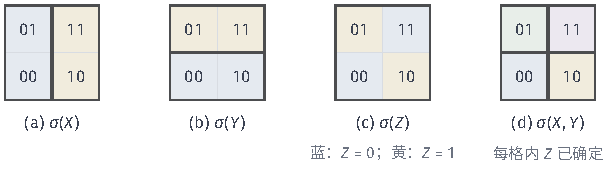
\includegraphics[width=104mm]{figures/02-abstract-mathematics/02-probability-spaces/tikz/pmod-xor-partitions/figure.pdf}
  \caption{两个独立公平比特$X,Y$与$Z=X\oplus Y$生成的信息。四格分别表示样本点$xy$，各有概率$1/4$，第一位$x$为列、第二位$y$为行。(a)(b)(c) 依次为$\sigma(X)$、$\sigma(Y)$、$\sigma(Z)$的两个块（同色为一块，(c)中蓝色为$Z=0$，黄色为$Z=1$）；任两种划分交出四个各$1/4$的格子。(d) $\sigma(X,Y)$把四格全部分开，每格中$Z$已经确定，所以$Z$不能独立于$(X,Y)$。}
  \label{fig:pmod-xor-partitions}
\end{figure}

\subsection{联合分布的乘积分解}

\paragraph{生成族上的独立性判据}
按定义验证独立，要对$\sigma(X_i)$中的全部事件检查乘法公式，这通常做不到。
与测度唯一性一样，我们希望只在一个生成族上检查。

\begin{lemma}[生成族上的独立性判据]
\label{lem:pmod-pi-independence}
设$\mathcal G_1,\dots,\mathcal G_n$是$\mathcal F$的子$\sigma$代数，$\mathcal C_i$是对有限交封闭的集合族，$\Omega\in\mathcal C_i$，且$\sigma(\mathcal C_i)=\mathcal G_i$。
若对任意$C_i\in\mathcal C_i$（$i=1,\dots,n$）都有
$\mathbb P(C_1\cap\cdots\cap C_n)=\prod_{i=1}^n\mathbb P(C_i)$，
则$\mathcal G_1,\dots,\mathcal G_n$相互独立。
\end{lemma}

\begin{proof}
固定$C_2\in\mathcal C_2,\dots,C_n\in\mathcal C_n$，在$\mathcal G_1$上比较两个有限测度
\[
  \mu(A)=\mathbb P(A\cap C_2\cap\cdots\cap C_n),\qquad
  \nu(A)=\mathbb P(A)\prod_{i=2}^n\mathbb P(C_i).
\]
由假设，$\mu$与$\nu$在$\mathcal C_1$上相等；$\mathcal C_1$包含$\Omega$，对有限交封闭且生成$\mathcal G_1$，由定理~\ref{thm:measure-pi-lambda-uniqueness}，$\mu=\nu$在整个$\mathcal G_1$上成立。
于是乘法公式在$\mathcal C_1$换成$\mathcal G_1$后仍然成立。
对第二个坐标重复同样的论证（此时第一个坐标已可任取$\mathcal G_1$中的事件），依次进行$n$步，得到乘法公式对任意$A_i\in\mathcal G_i$成立。
最后，对子集$J\subseteq\{1,\dots,n\}$，在$i\notin J$处取$A_i=\Omega$，即得定义要求的每个有限子族的乘法公式。
\end{proof}

对无穷族$(\mathcal G_i)_{i\in I}$，只需对每个有限子族应用引理。

\paragraph{独立与乘积测度}
现在可以把独立性完全翻译成联合分布的性质。
概率测度是有限测度，第~\ref{sec:measure-general-structure}节保证有限个概率测度的乘积测度在乘积$\sigma$代数上存在且唯一，它由矩形上的取值$\prod_iP_i(B_i)$决定。

\begin{theorem}[独立与乘积分解]
\label{thm:pmod-independence-product}
设$X_1,\dots,X_n$定义在同一个概率空间上，$X_i$取值于$(E_i,\mathcal E_i)$。
则$X_1,\dots,X_n$相互独立，当且仅当在$\mathcal E_1\otimes\cdots\otimes\mathcal E_n$上
\[
  P_{(X_1,\dots,X_n)}=P_{X_1}\otimes\cdots\otimes P_{X_n}.
\]
\end{theorem}

\begin{proof}
可测矩形$R=B_1\times\cdots\times B_n$（$B_i\in\mathcal E_i$）构成的族对有限交封闭，包含整个乘积空间，并生成乘积$\sigma$代数。
在矩形上，
\[
  \begin{aligned}
  P_{(X_1,\dots,X_n)}(R)&=\mathbb P\Bigl(\bigcap_{i=1}^n\{X_i\in B_i\}\Bigr),\\
  (P_{X_1}\otimes\cdots\otimes P_{X_n})(R)&=\prod_{i=1}^n\mathbb P(X_i\in B_i).
  \end{aligned}
\]
若$X_1,\dots,X_n$独立，两式右侧相等，于是两个概率测度在矩形上相等；由定理~\ref{thm:measure-pi-lambda-uniqueness}，它们在整个乘积$\sigma$代数上相等。
反之，若两个测度相等，把它们作用于矩形即得$\mathbb P(\bigcap_i\{X_i\in B_i\})=\prod_i\mathbb P(X_i\in B_i)$对一切$B_i$成立；取部分$B_i=E_i$就得到每个子族的乘法公式。
\end{proof}

证明的关键在唯一性那一步。
独立性的定义只直接给出矩形事件的概率；乘积空间中的大多数事件，例如$\{X<Y\}$或$\{X^2+Y^2\le1\}$，都不是矩形。
定理说明，一旦矩形上的乘法公式成立，这些事件的概率也随之由乘积测度确定，可以用累次积分计算。

\begin{example}[两个独立均匀变量的比较]
\label{ex:pmod-independent-uniform-order}
设$X,Y$独立，都服从$[0,1)$上的均匀分布。
由定理~\ref{thm:pmod-independence-product}，$(X,Y)$的联合分布是单位正方形上的面积。
矩形事件$\{X\in[0.2,0.6),\,Y\in[0.5,0.9)\}$的概率是$0.4\times0.4=0.16$。
非矩形事件$\{X<Y\}$的概率要对乘积测度积分；按$x$切片，第~\ref{sec:measure-general-structure}节的Tonelli定理给出
\[
  \mathbb P(X<Y)=\int_0^1\mathbb P(Y>x)\,dx=\int_0^1(1-x)\,dx=\frac12.
\]
\end{example}

图~\ref{fig:pmod-product-rectangle}对照了两种事件。
左图的矩形面积等于两条边长之积，这正是独立性在矩形上的直接含义；右图的三角形不是矩形，它的面积来自乘积测度的唯一扩张，再按竖直切片累加。

\begin{figure}[htbp]
  \centering
  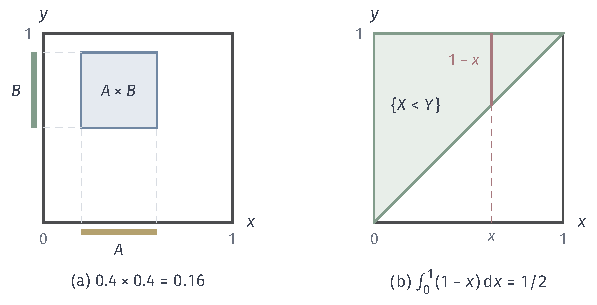
\includegraphics[width=100mm]{figures/02-abstract-mathematics/02-probability-spaces/tikz/pmod-product-rectangle/figure.pdf}
  \caption{$X,Y$独立且都服从$[0,1)$上的均匀分布时，联合分布为单位正方形上的面积。(a) 矩形$A\times B$，$A=[0.2,0.6)$，$B=[0.5,0.9)$，概率为边缘概率之积$0.16$；(b) 非矩形事件$\{X<Y\}$，在横坐标$x$处的切片长度为$1-x$，按切片积分得$1/2$。}
  \label{fig:pmod-product-rectangle}
\end{figure}

\paragraph{分布函数与密度判据}
对实值随机变量，生成族还可以进一步缩小。
半直线的原像$\{X_i\le a\}$（$a\in\mathbb R$）连同$\Omega$构成对有限交封闭的族；由于满足$X_i^{-1}(B)\in\sigma(\{X_i\le a\}:a\in\mathbb R)$的$B$构成包含全部半直线的$\sigma$代数，这一族生成$\sigma(X_i)$。
由引理~\ref{lem:pmod-pi-independence}，实值随机变量$X_1,\dots,X_n$相互独立，当且仅当
\begin{equation}
  \mathbb P(X_1\le a_1,\dots,X_n\le a_n)=\prod_{i=1}^n\mathbb P(X_i\le a_i)\qquad\text{对一切}\ a_1,\dots,a_n\in\mathbb R.
  \label{eq:pmod-cdf-factorization}
\end{equation}
（取部分$a_i\to+\infty$即得到含$\Omega$的情形。）
由分布函数的右连续性，只需对有理数$a_i$核对，再取有理数从右侧逼近即可。

若$(X,Y)$有联合密度$f$，独立等价于
\[
  f(x,y)=f_X(x)f_Y(y)\qquad\text{对几乎每个}\ (x,y)\in\mathbb R^2,
\]
其中$f_X,f_Y$是边缘密度。
若乘积式成立，Tonelli定理给出$\mathbb P(X\in A,Y\in B)=\int_Af_X\,dx\int_Bf_Y\,dy$，即独立；
反之，独立时联合分布等于$P_X\otimes P_Y$，后者在矩形上（从而由唯一性在全部Borel集上）以$f_X(x)f_Y(y)$为密度，同一测度的两个密度几乎处处相等（定理~\ref{thm:measure-radon-nikodym}）。
“几乎每个”不能去掉：在一条线段上改动$f$不改变任何概率。

乘积分解是独立的\emph{条件}，不是联合分布的一般形式。
例~\ref{ex:pmod-bernoulli-couplings}的同向与反向配对都有完全确定的联合分布，却不能写成边缘之积。

\subsection{独立性的保持与分组}

\paragraph{变换与分组}
实际中常把独立的观测分组汇总：先算前一半样本的均值，再算后一半样本的最大值。
我们希望知道，各组的汇总结果是否仍然独立。

\begin{theorem}[分组与变换保持独立]
\label{thm:pmod-independence-grouping}
设$(\mathcal G_i)_{i\in I}$是相互独立的子$\sigma$代数族，$I$被分成互不相交的子集$I_k$（$k\in K$）。令
$\mathcal H_k=\sigma\bigl(\bigcup_{i\in I_k}\mathcal G_i\bigr)$，则$(\mathcal H_k)_{k\in K}$相互独立。
特别地，若随机对象$(X_i)_{i\in I}$相互独立，各$I_k$有限，$f_k$是定义在$(X_i)_{i\in I_k}$取值空间上的可测函数，则$Y_k=f_k\bigl((X_i)_{i\in I_k}\bigr)$（$k\in K$）相互独立。
\end{theorem}

\begin{proof}
对每个$k$，令$\mathcal C_k$为形如$A_{i_1}\cap\cdots\cap A_{i_r}$的集合全体，其中$i_1,\dots,i_r$是$I_k$中有限个互不相同的指标，$A_{i_l}\in\mathcal G_{i_l}$；约定空交为$\Omega$。
两个这样的集合相交时，同一指标的事件在$\mathcal G_i$内相交，结果仍属于$\mathcal C_k$，所以$\mathcal C_k$对有限交封闭；它包含每个$\mathcal G_i$（$i\in I_k$），并含于$\mathcal H_k$，因此生成$\mathcal H_k$。

取有限个不同的$k_1,\dots,k_m$及$C_l\in\mathcal C_{k_l}$。
各$C_l$用到的指标属于不相交的$I_{k_l}$，所以$C_1\cap\cdots\cap C_m$是有限个来自不同$\mathcal G_i$的事件之交；由独立性，其概率等于所有这些事件概率之积。
把乘积按组归并，每组的乘积再由独立性等于$\mathbb P(C_l)$，于是
$\mathbb P(C_1\cap\cdots\cap C_m)=\prod_{l=1}^m\mathbb P(C_l)$。
由引理~\ref{lem:pmod-pi-independence}，$\mathcal H_{k_1},\dots,\mathcal H_{k_m}$相互独立；由于$k_1,\dots,k_m$是任取的有限个指标，整族$(\mathcal H_k)$相互独立。

对第二个结论，取$\mathcal G_i=\sigma(X_i)$。
$\sigma\bigl((X_i)_{i\in I_k}\bigr)$是包含各$\sigma(X_i)$的最小$\sigma$代数，即$\mathcal H_k$；由式~\eqref{eq:pmod-function-information}，$\sigma(Y_k)\subseteq\mathcal H_k$。
独立的$\sigma$代数的子$\sigma$代数仍满足乘法公式，所以$Y_k$相互独立。
\end{proof}

定理的第一个结论对组数和组的大小都没有有限性要求：可数多组、每组可数多个变量时，有限交组成的生成族和测度唯一性把乘法公式从有限个事件延伸到整个$\mathcal H_k$。
第二个结论要求各组有限，只是为了让$(X_i)_{i\in I_k}$取值于有限乘积空间；组内变量无穷时，任何$\mathcal H_k$可测的随机变量仍由第一个结论得到独立性。
例如$X_1,\dots,X_4$相互独立时，$X_1+X_2$与$X_3X_4$独立，$\max\{X_1,X_2\}$与$X_3$独立。
例~\ref{ex:pmod-xor-bits}正是从反面使用这个定理：把$\{X,Y\}$与$\{Z\}$分成两组，相互独立会迫使$\sigma(Z)$与$\sigma(X,Y)$独立，而概率为$1/2$的事件$\{Z=1\}$同属两者，这已经排除。

\paragraph{独立同分布族}
一族随机变量称为\term{独立同分布}（independent and identically distributed，i.i.d.），若它们相互独立并且服从同一个分布。
两个要求各管一件事：同分布只约束每个变量的边缘，独立约束它们的联合分布必须是边缘的乘积。
例~\ref{ex:pmod-alternating-bits}中的$Y_n$满足前者而不满足后者。

一个概率空间上能否容纳无穷多个独立的随机变量？$[0,1)$均匀模型就可以。

\begin{example}[二进制数字是独立的公平比特]
\label{ex:pmod-binary-digits}
对$\omega\in[0,1)$，令$d_k(\omega)=\lfloor2^k\omega\rfloor\bmod2$为它二进制展开（取不以无穷个$1$结尾的展开）的第$k$位。
对任意$n$及$b_1,\dots,b_n\in\{0,1\}$，事件$\{d_1=b_1,\dots,d_n=b_n\}$是一个长$2^{-n}$的二进区间，所以其概率为$2^{-n}$。
对$b_1,\dots,b_{n-1}$求和得$\mathbb P(d_n=b_n)=1/2$，于是
$\mathbb P(d_1=b_1,\dots,d_n=b_n)=\prod_{k=1}^n\mathbb P(d_k=b_k)$。
每个$\sigma(d_k)$只含$\varnothing,\{d_k=0\},\{d_k=1\},\Omega$四个事件，乘法公式在含$\Omega$的选取下由对相应$b_k$求和得到；由引理~\ref{lem:pmod-pi-independence}，$(d_k)_{k\ge1}$是独立同分布的$\operatorname{Bernoulli}(1/2)$序列。
\end{example}

例~\ref{ex:pmod-bernoulli-couplings}中的$X$与$Y^{(c)}$正是$d_1$与$d_2$，所以第三种配对是独立配对。
用这列数字还能造出更多对象：$\sum_k2d_k3^{-k}$服从第~\ref{sec:pmod-probability-space}节的Cantor分布；把数字分成无穷多组不相交的无穷子列，第$j$组的数字$d_{k_{j,1}},d_{k_{j,2}},\dots$重新排成$U_j=\sum_l d_{k_{j,l}}2^{-l}$，它与$\omega$本身同分布，即服从$[0,1)$上的均匀分布；$U_j$关于第$j$组生成的$\sigma$代数可测，由定理~\ref{thm:pmod-independence-grouping}的第一个结论，$U_1,U_2,\dots$相互独立。
本章研究的都是已经定义在给定概率空间上的随机族；由一套相容的有限维分布构造整个随机过程，以及一般指标集上的扩张定理，放在卷三“过程与轨迹演化”部分。

\section{期望与积分}
\label{sec:pmod-expectation}

卷一的期望有两种算法：离散时对概率表加权求和，有密度时对密度积分。
章首的等待时间两者都不适用。
本节把期望定义为对概率测度的积分，于是两种算法成为同一个定义的两种特例；再讨论矩条件控制了什么，以及几个后续章节反复使用的不等式。

\subsection{一般期望与分布积分}

\paragraph{期望的定义}
第~\ref{sec:measure-general-structure}节已经对一般测度定义了积分：非负函数的积分由简单函数从下逼近，可以取$+\infty$；有符号函数拆成正负两部分分别积分。
把它用于概率测度，就得到期望。

\begin{definition}[期望]
\label{def:pmod-expectation}
设$X$是概率空间$(\Omega,\mathcal F,\mathbb P)$上的随机变量。
若$X\ge0$，定义$\mathbb E X=\int_\Omega X\,d\mathbb P\in[0,+\infty]$。
一般情形记$X^+=\max\{X,0\}$，$X^-=\max\{-X,0\}$；当$\mathbb EX^+$与$\mathbb EX^-$不同时为$+\infty$时，定义$\mathbb EX=\mathbb EX^+-\mathbb EX^-$，称为$X$的\term{期望}（expectation）。
若$\mathbb E|X|<\infty$，称$X$\term{可积}（integrable）。
复值随机变量$X=U+\mathrm iV$在$\mathbb E|X|<\infty$时定义$\mathbb EX=\mathbb EU+\mathrm i\,\mathbb EV$。
\end{definition}

定义中的限制是为了排除$\infty-\infty$。
例如Cauchy分布的变量满足$\mathbb EX^+=\mathbb EX^-=+\infty$，它的期望没有定义；而一个非负变量的期望可以是$+\infty$，这时它是有定义的，只是不有限。
可积变量的期望具有线性与单调性，并且$|\mathbb EX|\le\mathbb E|X|$；对事件$A$，$\mathbb E\,\mathbb I_A=\mathbb P(A)$。
几乎必然相等的两个随机变量期望相同，因为积分不受零概率集合上取值的影响。

\paragraph{在取值空间上计算期望}
定义中的积分是在样本空间上进行的，可是实际计算时我们几乎从不知道$\Omega$的样子，只知道$X$的分布。
推前测度的积分公式把计算搬到取值空间。

\begin{theorem}[分布积分公式]
\label{thm:pmod-change-of-variables}
设$X$是取值于$(E,\mathcal E)$的随机对象，$g:E\to[0,+\infty]$可测，则
\[
  \mathbb E\,g(X)=\int_Eg\,dP_X.
\]
对可测的$g:E\to\mathbb R$，$g(X)$可积当且仅当$\int_E|g|\,dP_X<\infty$，此时上式仍成立。
\end{theorem}

\begin{proof}
这是式~\eqref{eq:measure-pushforward-integral}取$T=X$、$\mu=\mathbb P$的情形。
其机制是：$g=\mathbb I_B$时两边都等于$\mathbb P(X\in B)=P_X(B)$；由线性，等式对非负简单函数成立；用非负简单函数单调上升逼近$g$，两边同时应用单调收敛定理，得到非负情形。
有符号情形对$|g|$使用非负情形判断可积，再对$g^+$与$g^-$分别使用非负情形后相减。
\end{proof}

这个公式有两个直接推论。
第一，$\mathbb E\,g(X)$只依赖$P_X$：同分布的随机对象对一切非负或可积的$g$有相同期望，例~\ref{ex:pmod-reflection-uniform}中$\mathbb EX^2=\mathbb EY^2=1/3$。
第二，卷一的两种算法都是它的特例：$P_X=\sum_xp(x)\delta_x$时，由点质量混合的积分得$\mathbb Eg(X)=\sum_xg(x)p(x)$；$P_X$以$f$为密度时，$\int g\,dP_X=\int g(x)f(x)\,dx$，先对示性函数成立，再经简单函数与单调收敛推广。
对多个随机对象，把$g$取为乘积空间上的函数并用联合分布，就得到$\mathbb E\,g(X,Y)=\int g\,dP_{(X,Y)}$。

\paragraph{点质量与连续质量同时存在}
分布积分公式不要求$P_X$有任何特殊表示，因而可以直接处理混合分布。

\begin{example}[有空闲窗口的等待时间]
\label{ex:pmod-mixed-waiting}
设等待时间$X$以概率$0.4$等于$0$，以概率$0.6$服从率参数为$1$的指数分布，即
\[
  P_X=0.4\,\delta_0+0.6\,\mathrm{Exp}(1).
\]
它的分布函数在$x\ge0$时为$F_X(x)=0.4+0.6(1-e^{-x})$，在$0$处跳跃$0.4$。
积分对测度的混合是线性的，所以对非负可测$g$，
\[
  \mathbb E\,g(X)=0.4\,g(0)+0.6\int_0^\infty g(x)e^{-x}\,dx.
\]
取$g(x)=e^{-x}$，得$\mathbb Ee^{-X}=0.4+0.6\times\tfrac12=0.7$。
取$g(x)=x$与$x^2$，得$\mathbb EX=0.6$，$\mathbb EX^2=0.6\times2=1.2$，$\operatorname{Var}X=1.2-0.36=0.84$。
\end{example}

如果把$0.6e^{-x}$误当作$X$的密度，算出的$\mathbb Ee^{-X}$只有$0.3$，而且这个“密度”的总积分只有$0.6$。
图~\ref{fig:pmod-mixed-expectation}显示了遗漏的部分：左图的分布函数在原点有高$0.4$的跳跃，它就是点质量；右图中绿色面积$0.3$来自连续部分，红色竖线代表点质量贡献的$0.4\times g(0)=0.4$。
对$g(x)=x$，点质量的贡献是$0.4\times0=0$，所以只按连续部分算均值碰巧不出错；一旦$g(0)\ne0$，遗漏就会显现。

\begin{figure*}[htbp]
  \centering
  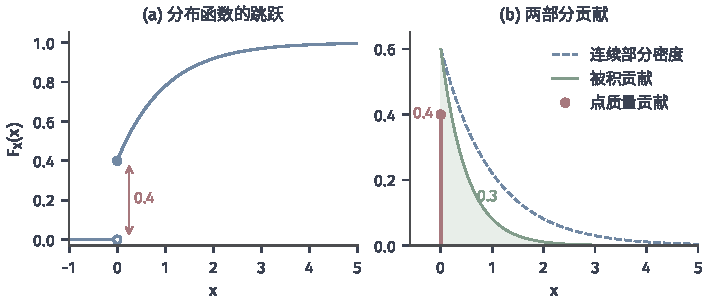
\includegraphics[width=120mm]{figures/02-abstract-mathematics/02-probability-spaces/matplotlib/pmod-mixed-expectation/figure.pdf}
  \caption{混合分布$P_X=0.4\delta_0+0.6\,\mathrm{Exp}(1)$的期望计算。(a) 分布函数在$x=0$处跳跃$0.4$，空心点为左极限；(b) 计算$\mathbb Ee^{-X}$时，虚线为连续部分的密度$0.6e^{-x}$，绿色区域为被积函数$0.6e^{-2x}$，面积$0.3$；红色竖线为点质量的贡献$0.4$。两部分之和为$0.7$。}
  \label{fig:pmod-mixed-expectation}
\end{figure*}

\paragraph{独立对象的乘积期望}
独立性使联合分布成为乘积测度，而乘积测度上的积分可以按坐标分别进行。

\begin{theorem}[独立对象的乘积期望]
\label{thm:pmod-product-expectation}
设$X$与$Y$独立，分别取值于$(E_1,\mathcal E_1)$与$(E_2,\mathcal E_2)$，$g:E_1\to\mathbb R$与$h:E_2\to\mathbb R$可测。
\begin{enumerate}
  \item 若$g,h\ge0$，则$\mathbb E[g(X)h(Y)]=\mathbb Eg(X)\,\mathbb Eh(Y)$，两边在$[0,+\infty]$中取值，约定$0\cdot\infty=0$。
  \item 若$g(X)$与$h(Y)$都可积，则$g(X)h(Y)$可积，且同一等式成立。
\end{enumerate}
特别地，独立可积实值随机变量满足$\mathbb E[XY]=\mathbb EX\,\mathbb EY$。
\end{theorem}

\begin{proof}
由定理~\ref{thm:pmod-change-of-variables}与定理~\ref{thm:pmod-independence-product}，
\[
  \mathbb E[g(X)h(Y)]=\int_{E_1\times E_2}g(x)h(y)\,d(P_X\otimes P_Y)(x,y).
\]
当$g,h\ge0$时，被积函数非负且乘积可测，第~\ref{sec:measure-general-structure}节的Tonelli定理允许先对$y$积分：内层积分为$g(x)\int h\,dP_Y$，外层再得$\int g\,dP_X\int h\,dP_Y$。
对第二条，先对$|g|,|h|$用第一条，得$\mathbb E|g(X)h(Y)|=\mathbb E|g(X)|\,\mathbb E|h(Y)|<\infty$；联合积分绝对有限，Fubini定理给出同样的累次积分分解。
\end{proof}

对有限个相互独立的随机对象，反复使用定理~\ref{thm:pmod-independence-grouping}与本定理即得$\mathbb E\prod_ig_i(X_i)=\prod_i\mathbb Eg_i(X_i)$。
没有独立性时等式一般不成立：在例~\ref{ex:pmod-bernoulli-couplings}的同向配对中，$\mathbb E[XY]=\mathbb EX^2=1/2$，而$\mathbb EX\,\mathbb EY=1/4$。
反过来，乘积期望分解也推不出独立：$\mathbb E[XY]=\mathbb EX\,\mathbb EY$只说明不相关，卷一已给出不相关却不独立的例子。

\subsection{矩与尾部控制}

\paragraph{矩记录尾部的累计}
随机变量取很大值的可能性，由\term{尾概率}（tail probability）$\mathbb P(|X|>t)$描述。
期望是否有限，取决于这些尾部在累计时是否收敛；不同幂次的累计给出不同强度的要求。
对$p>0$，称$\mathbb E|X|^p$为$X$的$p$阶\term{绝对矩}（absolute moment）；$\mathbb E|X|^p<\infty$时称$X$有有限$p$阶矩。

\begin{lemma}[尾积分公式]
\label{lem:pmod-tail-formula}
设$X\ge0$是随机变量，$p>0$，则
\[
  \mathbb EX^p=\int_0^\infty pt^{p-1}\,\mathbb P(X>t)\,dt,
\]
两边允许同为$+\infty$。
\end{lemma}

\begin{proof}
对每个$\omega$，$X(\omega)^p=\int_0^{X(\omega)}pt^{p-1}\,dt=\int_0^\infty pt^{p-1}\mathbb I_{\{t<X(\omega)\}}\,dt$。
函数$(\omega,t)\mapsto pt^{p-1}\mathbb I_{\{t<X(\omega)\}}$非负，并且关于$\mathcal F\otimes\mathcal B([0,\infty))$可测，因为集合$\{(\omega,t):X(\omega)-t>0\}$是可测函数$(\omega,t)\mapsto X(\omega)-t$的上水平集。
对$\mathbb P\otimes\text{长度}$应用Tonelli定理交换积分次序：
\[
  \mathbb EX^p=\int_\Omega\int_0^\infty pt^{p-1}\mathbb I_{\{t<X\}}\,dt\,d\mathbb P
  =\int_0^\infty pt^{p-1}\,\mathbb P(X>t)\,dt.
\]
\end{proof}

公式说明，$p$阶矩有限要求尾概率在乘以$t^{p-1}$后仍可积；$p$越大，对尾部衰减的要求越高。
低阶矩因此比高阶矩更容易有限。

\begin{theorem}[高阶矩蕴含低阶矩]
\label{thm:pmod-moment-monotone}
设$0<p<q$，$X$是随机变量。则$\mathbb E|X|^p\le1+\mathbb E|X|^q$；特别地，有限$q$阶矩蕴含有限$p$阶矩。
\end{theorem}

\begin{proof}
对实数$x$，若$|x|\le1$则$|x|^p\le1$；若$|x|>1$则$|x|^p\le|x|^q$。
所以$|x|^p\le1+|x|^q$对一切$x$成立，把$x$换成$X$并取期望即得。
这里用到概率空间的总质量为$1$：常数$1$的期望是$1$。
\end{proof}

于是有界变量的各阶矩都有限，有限二阶矩蕴含有限一阶矩，而一阶矩有限不能推出二阶矩有限。
本节最后一小节会用Jensen不等式给出更精细的比较。

\begin{example}[Pareto尾部与矩的存在性]
\label{ex:pmod-pareto-moments}
设$\alpha>0$，$X\ge1$满足$\mathbb P(X>t)=t^{-\alpha}$（$t\ge1$）。
由引理~\ref{lem:pmod-tail-formula}，
\[
  \mathbb EX^p=\int_0^1pt^{p-1}\,dt+\int_1^\infty pt^{p-1-\alpha}\,dt
  =\begin{cases}\dfrac{\alpha}{\alpha-p},&p<\alpha,\\[1ex] +\infty,&p\ge\alpha.\end{cases}
\]
例如$\alpha=2.5$时$\mathbb EX=5/3$，$\mathbb EX^2=5$，$\mathbb EX^3=+\infty$；$\alpha=1.5$时均值为$3$而方差为无穷。
\end{example}

图~\ref{fig:pmod-moment-tails}左图在对数坐标下画出三种尾概率，它们是斜率为$-\alpha$的直线：$\alpha$越小，尾部越重。
右图画出截断二阶矩$m_2(T)=\mathbb E[\min\{X,T\}^2]$随截断点$T$的变化。
$\alpha=4$与$\alpha=2.5$时曲线分别趋于$2$与$5$；$\alpha=1.5$时曲线按$T^{1/2}$的速度无限增长，二阶矩不存在。
矩条件保留的是这种累计层面的尾部信息：它说明尾部总体上衰减多快，但不规定尾概率曲线的具体形状。

\begin{figure*}[htbp]
  \centering
  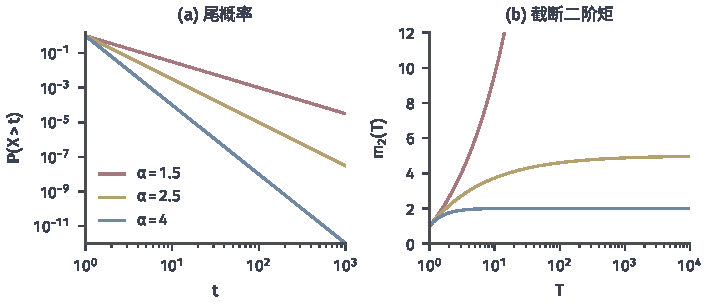
\includegraphics[width=120mm]{figures/02-abstract-mathematics/02-probability-spaces/matplotlib/pmod-moment-tails/figure.pdf}
  \caption{Pareto型尾部$\mathbb P(X>t)=t^{-\alpha}$（$t\ge1$），$\alpha=1.5,2.5,4$。(a) 双对数坐标下的尾概率，直线斜率为$-\alpha$；(b) 截断二阶矩$m_2(T)=\mathbb E[\min\{X,T\}^2]=1+2(T^{2-\alpha}-1)/(2-\alpha)$，横轴为对数尺度。$\alpha>2$时曲线收敛到$\mathbb EX^2=\alpha/(\alpha-2)$，$\alpha=1.5$时发散。}
  \label{fig:pmod-moment-tails}
\end{figure*}

\paragraph{Markov与Chebyshev不等式}
反过来，有限的矩可以控制尾概率。
这正是卷一Markov与Chebyshev不等式所做的事；它们只用到非负函数积分的单调性，所以在一般概率空间中原样成立。

\begin{theorem}[Markov与Chebyshev不等式]
\label{thm:pmod-markov}
设$X$是随机变量，$t>0$。
\begin{enumerate}
  \item 对任意$p>0$，$\mathbb P(|X|\ge t)\le\mathbb E|X|^p/t^p$。更一般地，若$h:[0,\infty)\to[0,\infty)$单调不减且$h(t)>0$，则$\mathbb P(|X|\ge t)\le\mathbb Eh(|X|)/h(t)$。
  \item 若$\mathbb EX^2<\infty$，则$\mathbb P(|X-\mathbb EX|\ge t)\le\operatorname{Var}X/t^2$。
\end{enumerate}
\end{theorem}

\begin{proof}
由$h$单调不减且非负，逐点有
$h(|X|)\ge h(t)\,\mathbb I_{\{|X|\ge t\}}$：$|X|\ge t$时右边为$h(t)\le h(|X|)$，否则右边为$0$。
对两边取期望，得$\mathbb Eh(|X|)\ge h(t)\,\mathbb P(|X|\ge t)$。
取$h(s)=s^p$得到\term{Markov不等式}（Markov inequality）的幂次形式；把$X$换成$X-\mathbb EX$并取$p=2$，得到\term{Chebyshev不等式}（Chebyshev inequality）。
\end{proof}

右边若为$+\infty$，不等式仍然成立，但不提供任何信息。
所以使用这些估计之前，必须先确认相应的矩有限；卷一在\BookChapterRef{chap:sampling-errors}{卷一“抽样分布与估计误差”章}中用它们证明了弱大数定律，后面的收敛章节也会以同样方式控制误差。

图~\ref{fig:pmod-markov-bounds}对$\alpha=3$的Pareto变量比较了三个矩界$\mathbb EX^p/t^p$与真实尾概率$t^{-3}$。
三个界都正确，但都远高于真实值：在$t=10$处，真实尾概率为$0.001$，$p=1,2,2.5$的界分别为$0.15$、$0.03$和约$0.019$。
阶数越高，界在大$t$处下降得越快；但常数$\mathbb EX^p=3/(3-p)$也越大，在$t=2$处$p=2.5$的界约为$1.06$，比平凡的上界$1$还差。
$p\ge3$时$\mathbb EX^p=\infty$，这一族界到此为止：矩界最多以多项式速度刻画尾部，系统的集中不等式留给\BookPartRef{part:inference-and-causal-identification}{卷四“推断与因果识别”部分}。

\begin{figure}[htbp]
  \centering
  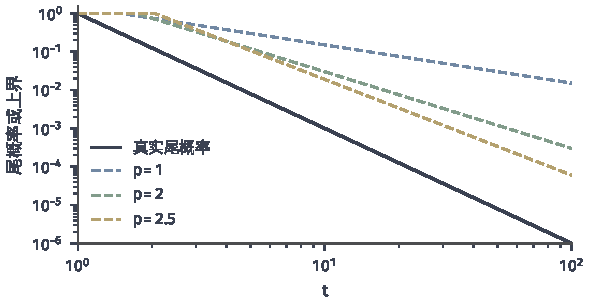
\includegraphics[width=100mm]{figures/02-abstract-mathematics/02-probability-spaces/matplotlib/pmod-markov-bounds/figure.pdf}
  \caption{$\alpha=3$的Pareto变量（$\mathbb P(X\ge t)=t^{-3}$，$t\ge1$）的真实尾概率（实线）与矩界$\min\{1,\mathbb EX^p/t^p\}$（虚线，$p=1,2,2.5$，$\mathbb EX^p=3/(3-p)$），双对数坐标。界始终在真实值之上；$p$越大，界在大$t$处越紧，在小$t$处可能更松。}
  \label{fig:pmod-markov-bounds}
\end{figure}

\subsection{随机向量的期望与协方差}

\paragraph{逐坐标的期望}
对随机向量$\bm X=(X_1,\dots,X_d)^\top$，若每个坐标可积，定义$\mathbb E\bm X=(\mathbb EX_1,\dots,\mathbb EX_d)^\top$；随机矩阵同样逐元素取期望。
坐标可积与范数可积是一回事：由
\[
  \max_i|x_i|\le\lVert\bm x\rVert_2\le\sum_{i=1}^d|x_i|,
\]
$\mathbb E\lVert\bm X\rVert_2<\infty$当且仅当每个$\mathbb E|X_i|<\infty$；有限维空间上各种范数彼此等价，选哪一种范数不影响结论。
期望的线性性逐坐标成立：对固定矩阵$\bm A$与向量$\bm b$，$\mathbb E[\bm A\bm X+\bm b]=\bm A\,\mathbb E\bm X+\bm b$，因为每个坐标都是有限个可积变量的线性组合。
这里只用到有限个实值积分，没有定义取值于一般Banach空间的随机对象的积分，也不需要函数空间的完备性。

\paragraph{乘积的可积性与Cauchy--Schwarz不等式}
协方差$\operatorname{Cov}(X,Y)=\mathbb E[(X-\mathbb EX)(Y-\mathbb EY)]$要求乘积可积。
由$2|xy|\le x^2+y^2$，$\mathbb EX^2$与$\mathbb EY^2$有限时$\mathbb E|XY|\le\tfrac12(\mathbb EX^2+\mathbb EY^2)<\infty$。
这个界还可以改进成乘积形式。

\begin{theorem}[Cauchy--Schwarz不等式]
\label{thm:pmod-cauchy-schwarz}
设随机变量$X,Y$满足$\mathbb EX^2<\infty$，$\mathbb EY^2<\infty$。则$XY$可积，且
\[
  \bigl(\mathbb E[XY]\bigr)^2\le\bigl(\mathbb E|XY|\bigr)^2\le\mathbb EX^2\,\mathbb EY^2.
\]
\end{theorem}

\begin{proof}
可积性已由上一段得到，第一个不等号是$|\mathbb E[XY]|\le\mathbb E|XY|$。
对实数$s$，展开非负随机变量的期望：
\[
  0\le\mathbb E\bigl(|X|-s|Y|\bigr)^2=\mathbb EX^2-2s\,\mathbb E|XY|+s^2\,\mathbb EY^2.
\]
若$\mathbb EY^2>0$，取$s=\mathbb E|XY|/\mathbb EY^2$，得$\mathbb EX^2-(\mathbb E|XY|)^2/\mathbb EY^2\ge0$，即所需结论。
若$\mathbb EY^2=0$，则$Y=0$几乎必然成立，$XY=0$几乎必然成立，两边都是$0$。
\end{proof}

取$X-\mathbb EX$与$Y-\mathbb EY$代入，得$|\operatorname{Cov}(X,Y)|\le\sqrt{\operatorname{Var}X\operatorname{Var}Y}$，所以有限二阶矩保证协方差有限；取$Y=1$，得$(\mathbb E|X|)^2\le\mathbb EX^2$。
这个不等式的思路与卷一用内积解释相关系数相同，这里补齐的是一般概率空间上的可积性。
本书称它为\term{Cauchy--Schwarz不等式}（Cauchy--Schwarz inequality），第~\ref{chap:conditional-expectation}章的条件均方误差和第~\ref{chap:weak-convergence-limit-theorems}章的多元极限都会使用它。

\paragraph{协方差矩阵的半正定性}
设$\mathbb E\lVert\bm X\rVert_2^2<\infty$，记$\bm\mu=\mathbb E\bm X$。
由上一段，每个$\operatorname{Cov}(X_i,X_j)$都有限，于是\term{协方差矩阵}（covariance matrix）
$\bm\Sigma=\mathbb E[(\bm X-\bm\mu)(\bm X-\bm\mu)^\top]$的每个元素都有定义。

\begin{theorem}[协方差矩阵半正定]
\label{thm:pmod-covariance-psd}
设$\bm X$是$d$维随机向量，$\mathbb E\lVert\bm X\rVert_2^2<\infty$。则对任意$\bm a\in\mathbb R^d$，
\[
  \bm a^\top\bm\Sigma\bm a=\operatorname{Var}(\bm a^\top\bm X)\ge0,
\]
因此$\bm\Sigma$是对称半正定矩阵。
\end{theorem}

\begin{proof}
$\bm a^\top\bm\Sigma\bm a=\sum_{i,j}a_ia_j\operatorname{Cov}(X_i,X_j)$，由期望对有限和的线性，这等于$\mathbb E\bigl[(\bm a^\top(\bm X-\bm\mu))^2\bigr]=\operatorname{Var}(\bm a^\top\bm X)$，非负。
对称性来自$\operatorname{Cov}(X_i,X_j)=\operatorname{Cov}(X_j,X_i)$。
\end{proof}

若某个$\bm a\ne\bm0$使$\bm a^\top\bm\Sigma\bm a=0$，则$\bm a^\top\bm X=\bm a^\top\bm\mu$几乎必然成立，$\bm X$几乎必然落在一个超平面内；协方差矩阵奇异并不违反任何定义。
定理把向量的二阶结构化为标量线性组合的方差，这是后面处理多元极限时的基本桥梁。
高斯向量协方差的具体计算见\BookChapterRef{chap:random-vectors}{卷一“随机向量与联合分布”章}，这里不再重复。

\subsection{凸函数与期望}

\paragraph{支撑直线与Jensen不等式}
先求平均再作非线性变换，与先变换再求平均，结果一般不同。
方差非负就是一个例子：$\mathbb EX^2-(\mathbb EX)^2=\operatorname{Var}X\ge0$，即$(\mathbb EX)^2\le\mathbb EX^2$。
对一般的凸函数，这种比较称为\term{Jensen不等式}（Jensen's inequality），比较的依据是\term{支撑直线}（supporting line）。

设$\varphi:\mathbb R\to\mathbb R$是\term{凸函数}（convex function）。
凸性使差商$(\varphi(x)-\varphi(m))/(x-m)$随$x$单调不减，所以右导数$c=\varphi'_+(m)$存在且有限；对$x>m$，差商不小于$c$，对$x<m$，差商不大于左导数$\varphi'_-(m)\le c$。
两种情形都给出
\begin{equation}
  \varphi(x)\ge\varphi(m)+c(x-m),\qquad x\in\mathbb R,
  \label{eq:pmod-support-line}
\end{equation}
即直线$\ell(x)=\varphi(m)+c(x-m)$在$m$处接触$\varphi$的图像，并处处位于图像下方。
有限凸函数是连续的，因而Borel可测，$\varphi(X)$是随机变量。

\begin{theorem}[Jensen不等式]
\label{thm:pmod-jensen}
设$X$是可积随机变量，$\varphi:\mathbb R\to\mathbb R$是凸函数。
则$\varphi(X)^-$可积，$\mathbb E\varphi(X)$在$(-\infty,+\infty]$中有定义，并且
\[
  \varphi(\mathbb EX)\le\mathbb E\varphi(X).
\]
\end{theorem}

\begin{proof}
取$m=\mathbb EX$，$\ell$为式~\eqref{eq:pmod-support-line}中的支撑直线，则逐点有$\varphi(X)\ge\ell(X)$。
于是$\varphi(X)^-\le\ell(X)^-\le|\varphi(m)|+|c|\,|X-m|$，右边可积，所以$\varphi(X)^-$可积，$\mathbb E\varphi(X)$有定义（可能为$+\infty$）。
由于$\varphi(X)-\ell(X)\ge0$且$\ell(X)$可积，
\[
  \mathbb E\varphi(X)\ge\mathbb E\ell(X)=\varphi(m)+c(\mathbb EX-m)=\varphi(\mathbb EX).
\]
\end{proof}

证明中先确认负部可积这一步不能省：否则$\mathbb E\varphi(X)$可能是未定义的$\infty-\infty$，比较大小无从谈起。
图~\ref{fig:pmod-jensen-support}以三点分布说明证明的几何含义。
$X$取$-1,0.5,2$，概率$0.3,0.5,0.2$，均值$\mu=0.35$。
支撑直线在$\mu$处接触$\varphi(x)=e^x$，直线上三点的加权平均恰好落回$\varphi(\mu)=e^{0.35}\approx1.42$；曲线上三点的加权平均$\mu_\varphi=\mathbb Ee^X\approx2.41$。
两者之差是曲线与支撑直线在各取值处竖直距离的加权平均。

\begin{figure}[htbp]
  \centering
  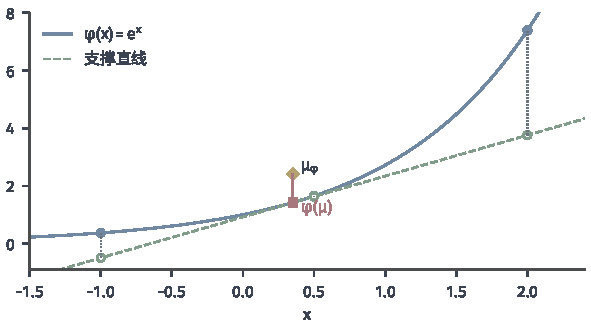
\includegraphics[width=100mm]{figures/02-abstract-mathematics/02-probability-spaces/matplotlib/pmod-jensen-support/figure.pdf}
  \caption{Jensen不等式的支撑直线论证。$X$取$-1,0.5,2$的概率分别为$0.3,0.5,0.2$，$\mu=\mathbb EX=0.35$。实线为$\varphi(x)=e^x$，虚线为它在$\mu$处的切线（支撑直线）。实心点为$(x_i,\varphi(x_i))$，空心点为直线上的对应点，点线为两者的竖直差距。方块为$\varphi(\mu)\approx1.42$，菱形为$\mu_\varphi=\mathbb E\varphi(X)\approx2.41$。}
  \label{fig:pmod-jensen-support}
\end{figure}

\paragraph{绝对值、幂次与等号条件}
取$\varphi(x)=|x|$得$|\mathbb EX|\le\mathbb E|X|$；取$\varphi(x)=|x|^p$（$p\ge1$）得$|\mathbb EX|^p\le\mathbb E|X|^p$。
Jensen不等式还给出定理~\ref{thm:pmod-moment-monotone}的精细版本。
设$0<p<q$且$\mathbb E|X|^q<\infty$；由该定理$Y=|X|^p$可积，对凸函数$\varphi(y)=|y|^{q/p}$应用Jensen不等式，得
\[
  \bigl(\mathbb E|X|^p\bigr)^{q/p}\le\mathbb E|X|^q,\qquad\text{即}\qquad
  \bigl(\mathbb E|X|^p\bigr)^{1/p}\le\bigl(\mathbb E|X|^q\bigr)^{1/q}.
\]
在概率空间上，$p\mapsto(\mathbb E|X|^p)^{1/p}$单调不减：阶数越高，这种“平均大小”越不会变小。这一步用到总质量为$1$，对一般测度并不成立。

等号何时成立？
若$\varphi$严格凸，则支撑直线只在$m$处接触图像，$x\ne m$时$\varphi(x)>\ell(x)$。
当$\mathbb E\varphi(X)=\varphi(\mathbb EX)$且有限时，非负变量$\varphi(X)-\ell(X)$的期望为零，因此几乎必然为零，从而$X=\mathbb EX$几乎必然成立：严格凸函数的等号只属于几乎必然为常数的变量。
$|x|$不是严格凸的，它的等号条件更宽：$|\mathbb EX|=\mathbb E|X|$当且仅当$X$几乎必然不变号。
例如$\mathbb EX\ge0$时，等式意味着$\mathbb E(|X|-X)=0$，而$|X|-X\ge0$，所以$|X|=X$几乎必然成立。
给定部分信息后的条件版本是第~\ref{chap:conditional-expectation}章的定理~\ref{thm:cond-jensen}。

\section{本章小结}
\label{sec:pmod-summary}

本章把概率计算分成三个层次。
第一层是概率空间上的随机对象：$(\Omega,\mathcal F,\mathbb P)$给出可能结果、允许判断的事件及其概率，随机对象是可测映射，它生成的$\sigma(X)$说明观测能分辨哪些事件。

第二层是取值空间上的分布：$P_X=X_\#\mathbb P$只保留各取值集合上的概率，舍弃了“哪个结果给出哪个值”，所以同分布的变量可以处处不相等，相同边缘的随机变量列可以有完全不同的样本轨迹。
多个对象一起出现的规律由联合分布记录，边缘分布只是它的投影；独立性要求联合分布恰好分解为边缘的乘积测度，这一条件只需在生成族上核对，并在不相交的分组与可测变换后保持。

第三层是对分布的累计：期望是对$\mathbb P$的积分，又可以通过分布积分公式在取值空间上计算，因而点质量、密度和两者的混合都用同一个公式处理；矩条件记录尾部累计的可积程度，Markov、Cauchy--Schwarz与Jensen不等式在相应矩有限时控制尾概率、乘积与非线性变换。

回到章首的问题。
三位骰子记录员面对同一个概率空间，区别在于各自记录生成的$\sigma$代数；有空闲窗口的等待时间可以直接对混合分布积分，得到$\mathbb EX=0.6$；同分布与相同边缘都只描述取值空间上的规律，不能决定样本点上的相等、收敛或共同发生。
不过，现在我们只能说清“已知的信息是什么”，还不能在只掌握部分信息时给出保持正确累计的平均值，例如只知道点数和时，第一枚骰子的平均点数应当是多少。
第~\ref{chap:conditional-expectation}章由此建立条件期望与条件分布；随后两章分别研究同一概率空间上随机变量列的收敛，以及只比较取值空间上分布的弱收敛，本章区分的样本点与分布两个层次将在那里分别成为两类收敛的出发点。

\chapter{条件期望与条件分布}
\label{chap:conditional-expectation}

设想一台传感器只报告目标落在哪个区段，而不报告精确位置；或者一个分类器只看到图像的几项特征，看不到生成图像的全部细节。
我们仍想根据已有的观测，给出某个数值量的最好平均估计，甚至给出它在当前观测下的整个概率分布。
当观测只有有限个取值时，做法很朴素：把样本点按观测值分组，组内求平均，组内的频率归一化后就是条件分布。
可是观测一旦取连续值，每个具体取值$\{Y=y\}$的概率都是零，“组内总量除以组的概率”变成了$0/0$。
那么给定$Y=y$时的平均值究竟指什么？它在多大程度上被唯一确定？能否用同一个对象同时给出所有事件的条件概率？

本章用两项要求回答第一个问题：条件平均只能使用已有的信息，并且在每个可以观察的事件上保持原变量的积分总量。
这两项要求不涉及任何除法，因此对零概率的观测值同样有意义；第~\ref{chap:densities-change-of-measure}章的Radon--Nikodym定理保证满足它们的随机变量存在，并且几乎处处唯一。
随后我们从这两项要求推出条件期望的运算规则、嵌套信息下的塔式法则、条件均方误差的分解，以及固定信息下交换条件期望与极限的条件。

第二个问题需要换一个对象。
条件期望逐个处理可积变量，每个事件的条件概率各自只在几乎处处意义下确定；要让它们在每个观测值处拼成一个概率分布，需要“输入一个状态、输出一个概率分布”的概率核。
因此我们先独立建立概率核及其积分、联合分布与复合，再用它定义条件分布，讨论存在所需的空间条件、不同版本之间的关系，以及条件密度与Bayes公式。
最后，条件分布让我们能够准确表达“给定已有信息后，另一项观测是否还会改变分布”，这就是条件独立。

\section{信息与条件平均}
\label{sec:cond-information}

本节从只能看到分组的情形出发，确定条件平均应当满足什么要求，再用子$\sigma$代数描述“可用信息”。
这里只建立问题；生成$\sigma$代数等记号沿用第~\ref{chap:probability-models}章。

\subsection{分组观察与条件平均}

\paragraph{只看到分组时的平均}
设$(\Omega,\mathcal F,\mathbb P)$是有限概率空间，$X$是其上的随机变量。
假设观察者只能确定样本点落在划分$A_1,\ldots,A_m$中的哪一块，看不到块内的细节。
对$\mathbb P(A_i)>0$的块，最自然的估计是组内平均
\begin{equation}
  \frac{\mathbb E[X\mathbb I_{A_i}]}{\mathbb P(A_i)}=\frac{1}{\mathbb P(A_i)}\sum_{\omega\in A_i}X(\omega)\mathbb P(\{\omega\}).
  \label{eq:cond-group-average}
\end{equation}
把每一块上的组内平均放回该块，就得到一个在各块上取常值的随机变量$Z$：样本点落在$A_i$时，$Z$取式~\eqref{eq:cond-group-average}的值。

\begin{example}[四点空间上的分组平均]
\label{ex:cond-four-points}
取$\Omega=\{0,2,4,6\}$，四个样本点各有概率$1/4$，令$X(\omega)=\omega$。
观察只告诉我们样本点属于$A_1=\{0,2\}$还是$A_2=\{4,6\}$。
由式~\eqref{eq:cond-group-average}，
\[
  \frac{\mathbb E[X\mathbb I_{A_1}]}{\mathbb P(A_1)}=\frac{(0+2)/4}{1/2}=1,\qquad
  \frac{\mathbb E[X\mathbb I_{A_2}]}{\mathbb P(A_2)}=\frac{(4+6)/4}{1/2}=5.
\]
于是$Z(0)=Z(2)=1$，$Z(4)=Z(6)=5$。
\end{example}

图~\ref{fig:cond-four-points}把这一计算画了出来。
圆点是$X$在四个样本点上的值，粗横线是组内平均。
观察者看不到组内的差别，所以$Z$在每组上是一条水平线；它把组内的起伏抹平了，但没有改变每组的“总量”。

\begin{figure}[htbp]
  \centering
  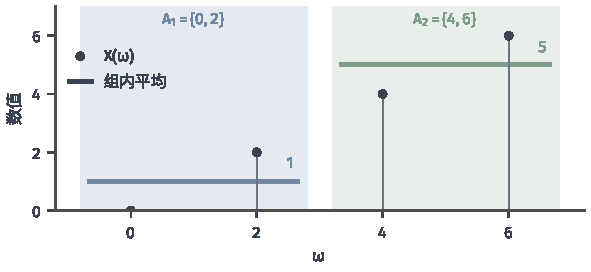
\includegraphics[width=100mm]{figures/02-abstract-mathematics/02-probability-spaces/matplotlib/cond-four-points/figure.pdf}
  \caption{四点空间上的分组平均。样本空间$\Omega=\{0,2,4,6\}$，每点概率$1/4$，圆点和竖线给出$X(\omega)=\omega$。蓝色与绿色底色分别是只能辨认的两组$A_1=\{0,2\}$和$A_2=\{4,6\}$，粗横线是组内平均$1$和$5$，它们合起来就是条件平均$Z$。}
  \label{fig:cond-four-points}
\end{figure}

\paragraph{条件平均保留的两项性质}
$Z$有两项性质值得单独写出。
第一，$Z$在每一块上取常值，因此只要知道样本点落在哪一块，就能确定$Z$的值；它只使用分组信息。
第二，在每一块上，$Z$与$X$的积分总量相同：
\[
  \mathbb E[Z\mathbb I_{A_i}]=\frac{\mathbb E[X\mathbb I_{A_i}]}{\mathbb P(A_i)}\,\mathbb P(A_i)=\mathbb E[X\mathbb I_{A_i}].
\]
在示例~\ref{ex:cond-four-points}中，两边分别是$1\times\frac12=\frac12$与$\frac{0+2}{4}=\frac12$。

观察者能够判断是否发生的事件，不只是单独的块，还有若干块的并。
由于积分对不交并可加，第二项性质对任意若干块的并同样成立；取全部块的并$\Omega$，得到$\mathbb EZ=\mathbb EX$，在示例中两边都是$3$。
这两项性质——只依赖可用信息、在每个可观察事件上保持积分——就是下一节抽象定义要保留的全部内容。

还有一个细节。
若某块$A_i$的概率为零，式~\eqref{eq:cond-group-average}无法计算；但无论在$A_i$上给$Z$赋什么值，$\mathbb E[Z\mathbb I_A]$对任何事件$A$都不变。
因此零概率分组上的赋值不影响上述两项性质，我们暂不为它规定唯一答案。

\subsection{子$\sigma$代数与可用信息}

\paragraph{用子$\sigma$代数表示可辨认的事件}
第~\ref{chap:probability-models}章用生成$\sigma$代数$\sigma(Y)$（定义~\ref{def:pmod-generated-sigma}）记录观测$Y$能够回答的全部“是否发生”问题。
一般地，我们用子$\sigma$代数$\mathcal G\subseteq\mathcal F$表示允许辨认的事件：$A\in\mathcal G$意味着观察者能判断$A$是否发生。
对$\mathcal G$可测的随机变量，其每个水平事件$\{Z\leq c\}$都在$\mathcal G$中，因而可以完全依据这些信息确定。
在有限划分的情形，$\mathcal G$由各块的全部并组成，$\mathcal G$可测恰好意味着在每一块上取常值，这正是上一小节的第一项性质。

信息的多少由事件族的包含关系衡量，而不是由观测的维数衡量。
若$\mathcal H\subseteq\mathcal G$，凡是用$\mathcal H$能判断的事件用$\mathcal G$也能判断，我们说$\mathcal G$比$\mathcal H$含有更多信息。
二维观测$(Y,2Y)$与一维观测$Y$生成同一个$\sigma$代数，因此信息相同；反过来，在$\Omega=[0,1)$（取$\mathcal F$为Borel $\sigma$代数）上，一维的恒等映射$\omega\mapsto\omega$就生成全部Borel事件，已经是完全信息。

图~\ref{fig:cond-information-layers}在$\Omega=[0,1)$（概率为长度）上比较四个逐步加细的信息。
取$X(\omega)=2\omega+\sin(2\pi\omega)$。
只知道“某事发生了”时，最好的平均只能是常数$\mathbb EX=1$；把区间分成两块、四块后，组内平均变成两级、四级阶梯；完全信息下，条件平均就是$X$本身。
信息越细，阶梯越贴近原函数，但每一级阶梯始终只依赖当前能辨认的块。

\begin{figure*}[htbp]
  \centering
  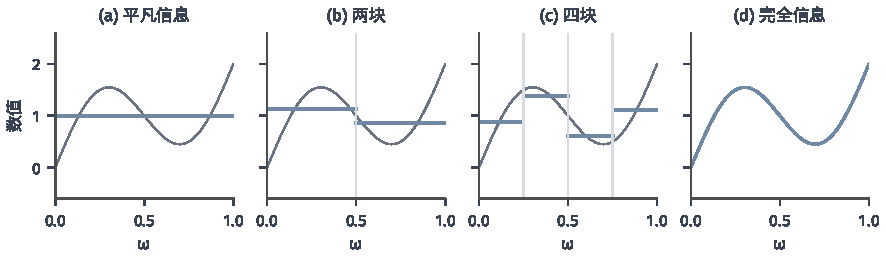
\includegraphics[width=150mm]{figures/02-abstract-mathematics/02-probability-spaces/matplotlib/cond-information-layers/figure.pdf}
  \caption{四种信息下的条件平均。样本空间为$[0,1)$，概率为长度；灰线是$X(\omega)=2\omega+\sin(2\pi\omega)$，蓝线是给定信息下的条件平均。(a)平凡信息，条件平均为常数$\mathbb EX=1$；(b)按$[0,\frac12),[\frac12,1)$分组，组内平均约为$1.137,0.863$；(c)按四个等长区间分组，组内平均约为$0.887,1.387,0.613,1.113$；(d)完全信息，条件平均与$X$重合。组内平均用$200000$个中点格点数值积分得到。}
  \label{fig:cond-information-layers}
\end{figure*}

\paragraph{两个极端与连续观测的困难}
两个极端情形可以直接从两项性质读出答案。
平凡$\sigma$代数$\{\varnothing,\Omega\}$只允许判断“某事发生了”，对它可测的随机变量只有常数；在$A=\Omega$上保持积分，要求这个常数等于$\mathbb EX$。
另一端$\mathcal G=\mathcal F$允许辨认全部事件，$X$本身就满足两项性质，条件平均应当是$X$。

有限划分的做法却不能直接搬到连续观测。
若$Y$服从标准正态分布，每个$\{Y=y\}$的概率都是零，式~\eqref{eq:cond-group-average}的分母为零；而$\sigma(Y)$中的事件$\{Y\in B\}$有不可数多个，也不能把它们看成有限个块的并。
于是自然的问题是：能否只保留“对$\mathcal G$可测”和“在$\mathcal G$的每个事件上保持积分”这两项要求，而完全不做逐组除法？
下一节说明这样做不仅可行，而且结果几乎处处唯一。

\section{条件期望的定义与存在性}
\label{sec:cond-definition}

本节固定概率空间$(\Omega,\mathcal F,\mathbb P)$与子$\sigma$代数$\mathcal G\subseteq\mathcal F$。
我们先把上一节的两项要求写成定义，再用Radon--Nikodym定理证明满足要求的随机变量存在，最后把抽象的信息$\mathcal G$换回具体的观测$Y$。

\subsection{条件期望的定义}

\paragraph{两项要求的一般形式}
上一节的两项性质不涉及除法，可以原样推广到任意子$\sigma$代数。

\begin{definition}[条件期望]
\label{def:cond-expectation}
设$X$是可积的实值随机变量，$\mathcal G\subseteq\mathcal F$是子$\sigma$代数。
若可积随机变量$Z$满足
\begin{enumerate}
  \item $Z$对$\mathcal G$可测；
  \item 对每个$A\in\mathcal G$，
  \begin{equation}
    \mathbb E[Z\mathbb I_A]=\mathbb E[X\mathbb I_A],
    \label{eq:cond-defining-identity}
  \end{equation}
\end{enumerate}
则称$Z$为$X$给定$\mathcal G$的\term{条件期望}（conditional expectation），记作$\mathbb E[X\mid\mathcal G]$。
\end{definition}

第一项条件说$Z$只使用$\mathcal G$中的信息，第二项条件说在每个可以观察的事件上，$Z$与$X$有相同的积分总量。
对有限划分生成的$\mathcal G$，上一节已经验证分组平均满足这两项条件：$\mathcal G$中的事件是若干块的并，而式~\eqref{eq:cond-defining-identity}对每一块成立，从而对它们的不交并也成立。
因此示例~\ref{ex:cond-four-points}中的$Z$就是$\mathbb E[X\mid\mathcal G]$，其中$\mathcal G=\{\varnothing,A_1,A_2,\Omega\}$。

\paragraph{版本与条件概率}
条件期望是一个随机变量，而不是一个数。
下一小节将证明，满足定义的两个随机变量几乎必然相等（几乎必然的含义见定义~\ref{def:pmod-almost-sure}）；反过来，在$\mathcal G$中的零概率事件上改动$Z$，两项条件仍然成立。
所以定义确定的是一个几乎处处等价类，其中每一个具体的随机变量称为条件期望的一个版本。
写$\mathbb E[X\mid\mathcal G]=W$时，意思是$W$是一个版本；涉及条件期望的等式和不等式，默认都在几乎必然意义下成立。

取$X=\mathbb I_B$（$B\in\mathcal F$），就得到事件的条件概率
\[
  \mathbb P(B\mid\mathcal G)=\mathbb E[\mathbb I_B\mid\mathcal G].
\]
它满足$\mathbb E[\mathbb P(B\mid\mathcal G)\mathbb I_A]=\mathbb P(A\cap B)$对每个$A\in\mathcal G$成立，这正是“组内频率乘以组的概率等于交事件概率”的一般形式。
对有限维可积随机向量$\bm X=(X_1,\ldots,X_d)$，逐坐标定义$\mathbb E[\bm X\mid\mathcal G]$即可。
一般取值空间中的随机对象不一定能求平均，例如取值于一个没有线性结构的集合；它们的条件规律要用第~\ref{sec:cond-distributions}节的条件分布描述。

\subsection{条件期望的存在性与唯一性}

\paragraph{把积分总量看成测度}
定义只说了条件期望应当满足什么，还没有说明这样的随机变量一定存在。
关键的观察是：等式~\eqref{eq:cond-defining-identity}的右边$A\mapsto\mathbb E[X\mathbb I_A]$在$X\geq0$时是$\mathcal G$上的一个有限测度，而左边要求它由某个$\mathcal G$可测函数作为密度给出。
这正是Radon--Nikodym定理（定理~\ref{thm:density-radon-nikodym}）回答的问题：若$\sigma$有限测度$\nu$关于$\sigma$有限测度$\mu$绝对连续，则存在非负可测函数$f$使$\nu(A)=\int_Af\,d\mu$对每个可测集$A$成立。

需要注意的是，这里两个测度都只定义在$\mathcal G$上。
$X$本身一般不对$\mathcal G$可测，因此$X$不是所求的密度；密度定理在较小的$\sigma$代数上重新寻找一个$\mathcal G$可测的密度，这一步正是“只用可用信息”的数学体现。

\begin{theorem}[条件期望的存在性与唯一性]
\label{thm:cond-existence}
设$X$是可积随机变量，$\mathcal G\subseteq\mathcal F$是任意子$\sigma$代数。
则$\mathbb E[X\mid\mathcal G]$存在；若$Z_1,Z_2$都满足定义~\ref{def:cond-expectation}，则$Z_1=Z_2$几乎必然成立。
\end{theorem}

\begin{proof}
\emph{非负情形的存在性。}
先设$X\geq0$。在可测空间$(\Omega,\mathcal G)$上定义
\[
  \nu(A)=\mathbb E[X\mathbb I_A],\qquad A\in\mathcal G.
\]
若$A_1,A_2,\ldots\in\mathcal G$两两不交，则$\mathbb I_{\bigcup_kA_k}=\sum_k\mathbb I_{A_k}$，对非负部分和用单调收敛定理得$\nu(\bigcup_kA_k)=\sum_k\nu(A_k)$；又$\nu(\Omega)=\mathbb EX<\infty$，所以$\nu$是有限测度。
记$\mathbb P|_{\mathcal G}$为$\mathbb P$在$\mathcal G$上的限制，它是$(\Omega,\mathcal G)$上的概率测度。
若$A\in\mathcal G$且$\mathbb P(A)=0$，则非负随机变量$X\mathbb I_A$几乎必然为零，故$\nu(A)=0$；这说明$\nu\ll\mathbb P|_{\mathcal G}$。
两个测度都有限，由Radon--Nikodym定理，存在$\mathcal G$可测的非负函数$Z$，使
\[
  \nu(A)=\int_AZ\,d\mathbb P|_{\mathcal G},\qquad A\in\mathcal G.
\]
对$\mathcal G$可测的非负函数，关于$\mathbb P|_{\mathcal G}$与关于$\mathbb P$的积分相同：两者在$\mathcal G$中事件的示性函数上一致，从而在$\mathcal G$可测简单函数上一致，再由单调收敛推广到非负$\mathcal G$可测函数。
于是$\mathbb E[Z\mathbb I_A]=\mathbb E[X\mathbb I_A]$对每个$A\in\mathcal G$成立。取$A=\Omega$得$\mathbb EZ=\mathbb EX<\infty$，所以$Z$可积，它满足定义~\ref{def:cond-expectation}。

\emph{一般情形的存在性。}
对一般可积$X$，写$X=X^+-X^-$，其中$X^+=\max(X,0)$、$X^-=\max(-X,0)$都非负可积。
由上一步分别得到$Z^+=\mathbb E[X^+\mid\mathcal G]$与$Z^-=\mathbb E[X^-\mid\mathcal G]$，令$Z=Z^+-Z^-$。
$Z$对$\mathcal G$可测且可积，并且对每个$A\in\mathcal G$，
\[
  \mathbb E[Z\mathbb I_A]=\mathbb E[Z^+\mathbb I_A]-\mathbb E[Z^-\mathbb I_A]=\mathbb E[X^+\mathbb I_A]-\mathbb E[X^-\mathbb I_A]=\mathbb E[X\mathbb I_A].
\]
这里先拆开正负部分，是因为有符号的$A\mapsto\mathbb E[X\mathbb I_A]$不是非负测度，不能直接套用密度定理。

\emph{唯一性。}
设$Z_1,Z_2$都满足定义。事件$A=\{Z_1>Z_2\}$由两个$\mathcal G$可测函数确定，所以$A\in\mathcal G$。由式~\eqref{eq:cond-defining-identity}，
\[
  \mathbb E[(Z_1-Z_2)\mathbb I_A]=\mathbb E[X\mathbb I_A]-\mathbb E[X\mathbb I_A]=0.
\]
被积函数$(Z_1-Z_2)\mathbb I_A$非负且积分为零，因而几乎必然为零；而它在$A$上严格为正，所以$\mathbb P(A)=0$。
交换$Z_1,Z_2$的角色得$\mathbb P(Z_2>Z_1)=0$，故$Z_1=Z_2$几乎必然成立。
\end{proof}

\paragraph{这一论证不需要的条件}
证明对$\mathcal G$没有任何额外要求：它不必由可数个事件生成，样本空间也不必是标准Borel空间。
用到的只有两点：$\mathcal G$上的有限测度可以用密度表示，以及$\{Z_1>Z_2\}$这类事件本身就在$\mathcal G$中。
后面把全部事件的条件概率组织成一个分布时，空间结构的条件才会出现；那是另一个问题，不影响逐个可积变量的条件期望。

\paragraph{只在生成族上检验}
实际验证某个$W$是条件期望时，$\mathcal G$中的事件往往太多，无法逐个检查。
下面的引理说明，只需在一个对有限交封闭、且包含$\Omega$的生成族上检验等式~\eqref{eq:cond-defining-identity}。

\begin{lemma}[生成族上的检验]
\label{lem:cond-pi-check}
设$X$可积，$W$可积且对$\mathcal G$可测。若$\mathcal C$是生成$\mathcal G$的$\pi$系统，$\Omega\in\mathcal C$，并且$\mathbb E[W\mathbb I_C]=\mathbb E[X\mathbb I_C]$对每个$C\in\mathcal C$成立，则$W=\mathbb E[X\mid\mathcal G]$。
\end{lemma}

\begin{proof}
令$\mathcal D=\{A\in\mathcal G:\mathbb E[W\mathbb I_A]=\mathbb E[X\mathbb I_A]\}$，则$\mathcal C\subseteq\mathcal D$。
若$A\in\mathcal D$，由$\Omega\in\mathcal D$及$\mathbb I_{A^c}=1-\mathbb I_A$得$A^c\in\mathcal D$。
若$A_1,A_2,\ldots\in\mathcal D$两两不交，记$A=\bigcup_kA_k$，则$\sum_{k\leq n}W\mathbb I_{A_k}\to W\mathbb I_A$，且绝对值被可积的$|W|$控制，由控制收敛定理和$X$的同样论证得$A\in\mathcal D$。
因此$\mathcal D$对补集和不交可数并封闭。由$\pi$--$\lambda$定理（定理~\ref{thm:measure-pi-lambda}），包含$\pi$系统$\mathcal C$的这类集合族必包含$\sigma(\mathcal C)=\mathcal G$。
\end{proof}

\subsection{给定随机变量的条件期望}

\paragraph{观测值上的函数}
实际问题中的信息通常来自一个观测$Y$，它取值于可测空间$(E,\mathcal E)$。
我们定义
\[
  \mathbb E[X\mid Y]=\mathbb E[X\mid\sigma(Y)].
\]
它是$\sigma(Y)$可测的随机变量。
为了说出“给定$Y=y$时的平均”，需要把这样的随机变量写成观测值的函数；下面的结论通常称为\term{Doob--Dynkin引理}。

\begin{theorem}[Doob--Dynkin引理]
\label{thm:cond-doob-dynkin}
设$Y$取值于可测空间$(E,\mathcal E)$，$Z$是实值随机变量。
则$Z$对$\sigma(Y)$可测，当且仅当存在可测函数$h:E\to\mathbb R$，使$Z=h(Y)$在$\Omega$上处处成立。
\end{theorem}

\begin{proof}
若$Z=h(Y)$，则对每个Borel集$B$，$\{Z\in B\}=\{Y\in h^{-1}(B)\}\in\sigma(Y)$，所以$Z$对$\sigma(Y)$可测。

反过来，先设$Z=\mathbb I_A$，$A\in\sigma(Y)$。由$\sigma(Y)=\{\{Y\in B\}:B\in\mathcal E\}$，存在$B\in\mathcal E$使$A=\{Y\in B\}$，于是$Z=\mathbb I_B(Y)$。
对$\sigma(Y)$可测的简单函数$Z=\sum_ka_k\mathbb I_{A_k}$，逐项使用上一步并取线性组合即可。
对一般实值$\sigma(Y)$可测的$Z$，取$\sigma(Y)$可测简单函数$Z_n$逐点收敛到$Z$，并写$Z_n=h_n(Y)$。
令$L=\{y\in E:\lim_nh_n(y)\text{存在且有限}\}$，它由可数个可测函数的上、下极限确定，因而属于$\mathcal E$；定义$h(y)=\lim_nh_n(y)$（$y\in L$），在$L$外令$h(y)=0$，则$h$可测。
对每个$\omega$，$h_n(Y(\omega))=Z_n(\omega)\to Z(\omega)$，所以$Y(\omega)\in L$且$h(Y(\omega))=Z(\omega)$。
\end{proof}

证明中把$h$在$L$外补成零，是因为$h_n$只在$Y$实际取到的值上被$Z_n$约束，别处可能不收敛。
将定理用于$Z=\mathbb E[X\mid Y]$，得到可测函数$h$使$\mathbb E[X\mid Y]=h(Y)$，我们记
\[
  \mathbb E[X\mid Y=y]=h(y).
\]
这样，“给定$Y=y$后的条件平均”就有了准确含义：它是观测值上的一个函数，由积分条件
\begin{equation}
  \mathbb E[X\mathbb I_{\{Y\in B\}}]=\int_Bh(y)\,P_Y(dy),\qquad B\in\mathcal E
  \label{eq:cond-given-y-identity}
\end{equation}
刻画，右边用的是$Y$的分布$P_Y$和换元公式（定理~\ref{thm:pmod-change-of-variables}）。

$h$只在$P_Y$几乎处处的意义下确定。
若$h(Y)$与$h'(Y)$都是$\mathbb E[X\mid Y]$的版本，则$P_Y(\{h\neq h'\})=\mathbb P(h(Y)\neq h'(Y))=0$；反之，在一个$P_Y$零集上改动$h$，$h(Y)$只在一个零概率事件上改变，仍是一个版本。

\paragraph{离散观测与连续观测}
若$Y$只取有限个值$y_1,\ldots,y_m$，且每个$\mathbb P(Y=y_j)>0$，在式~\eqref{eq:cond-given-y-identity}中取$B=\{y_j\}$，得
\[
  h(y_j)=\frac{\mathbb E[X\mathbb I_{\{Y=y_j\}}]}{\mathbb P(Y=y_j)},
\]
这就回到第~\ref{sec:cond-information}节的分组平均，划分由$\{Y=y_j\}$给出。
卷一已经用这种按值分组的方式和普通密度计算过条件均值与全期望公式，本章的定义把那里的计算放进同一个框架，可参考\BookChapterRef{chap:random-vectors}{卷一“随机向量与联合分布”章}。

连续观测下，式~\eqref{eq:cond-given-y-identity}同样有意义，但它只约束$h$在$P_Y$意义下的“几乎所有”取值。
若$(X,Y)$有联合密度$p(x,y)$，在$0<p_Y(y)<\infty$且$\int|x|\,p(x,y)\,dx<\infty$处令$h(y)=\int x\,p(x,y)\,dx/p_Y(y)$，其余$y$处令$h(y)=0$。由$X$可积和Tonelli定理，被排除的$y$构成$P_Y$零集；再用Fubini定理可以验证$h$满足式~\eqref{eq:cond-given-y-identity}，因而是一个方便计算的版本。
但条件期望的定义与存在都不依赖联合密度，也从不把$\mathbb P(Y=y)=0$处的平均解释为两个零的比值。

\begin{example}[平方关系加独立噪声]
\label{ex:cond-square-noise}
设$Y\sim N(0,1)$，$\varepsilon\sim N(0,\sigma^2)$与$Y$独立，$X=Y^2+\varepsilon$。
我们直接用定义验证$h(y)=y^2$。
$h(Y)=Y^2$对$\sigma(Y)$可测且可积。对每个Borel集$B$，
\[
  \begin{aligned}
  \mathbb E[X\mathbb I_{\{Y\in B\}}]&=\mathbb E[Y^2\mathbb I_B(Y)]+\mathbb E[\varepsilon\,\mathbb I_B(Y)]\\
  &=\mathbb E[Y^2\mathbb I_B(Y)]+\mathbb E\varepsilon\cdot\mathbb P(Y\in B)=\mathbb E[Y^2\mathbb I_B(Y)],
  \end{aligned}
\]
第二个等号用了独立可积变量乘积的期望等于期望之积（定理~\ref{thm:pmod-product-expectation}）。
所以$\mathbb E[X\mid Y]=Y^2$，即$\mathbb E[X\mid Y=y]=y^2$。
\end{example}

图~\ref{fig:cond-regression-scatter}取$\sigma=0.5$，画出$600$个样本点$(Y,X)$。
如果把$Y$的取值范围切成宽$0.5$的小段，每一段就是一个正概率的组，组内平均（绿色短横线）是给定“$Y$落在哪一段”这一较粗信息的条件平均的经验估计。
这些短横线紧贴红色曲线$h(y)=y^2$。
不过要注意二者的关系：$h$不是由“分段越来越细”的极限定义的，而是由式~\eqref{eq:cond-given-y-identity}直接刻画；分段平均只是更粗信息下的条件平均，第~\ref{sec:cond-properties}节的塔式法则将说明它等于$h(Y)$在段内的平均。

\begin{figure}[htbp]
  \centering
  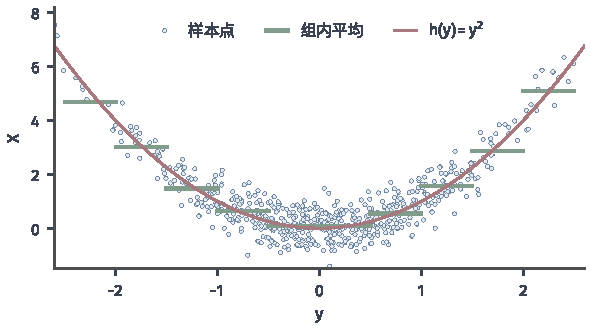
\includegraphics[width=100mm]{figures/02-abstract-mathematics/02-probability-spaces/matplotlib/cond-regression-scatter/figure.pdf}
  \caption{连续观测下的条件期望$\mathbb E[X\mid Y=y]=h(y)$。模型为$Y\sim N(0,1)$，$\varepsilon\sim N(0,0.25)$与$Y$独立，$X=Y^2+\varepsilon$；圆点为固定随机种子生成的$600$个样本，红线为$h(y)=y^2$，绿色短横线为$Y$按宽$0.5$分段后各段（至少含$5$个样本）的组内平均。}
  \label{fig:cond-regression-scatter}
\end{figure}

\section{条件期望的性质}
\label{sec:cond-properties}

有了定义和存在唯一性，我们分别研究条件期望的代数运算、信息嵌套、误差比较与极限交换。
各项性质的证明都回到同一个判定方法：先说明候选随机变量对当前信息可测，再检验它在可观察事件上的积分；唯一性（定理~\ref{thm:cond-existence}）随后保证它就是条件期望。

\subsection{条件期望的运算规则}

\paragraph{线性、保序与可测量保持}
组内平均对被平均的量是线性的：两个变量之和的组内平均等于各自组内平均之和；它也不会把逐点较小的量平均成较大的量。
下面的定理说明这些直观规则在一般情形下仍然成立，只是都附带“几乎必然”。

\begin{theorem}[条件期望的基本运算规则]
\label{thm:cond-rules}
设$X,X'$可积，$a,b\in\mathbb R$，$\mathcal G\subseteq\mathcal F$是子$\sigma$代数。则以下各式几乎必然成立：
\begin{enumerate}
  \item 线性：$\mathbb E[aX+bX'\mid\mathcal G]=a\,\mathbb E[X\mid\mathcal G]+b\,\mathbb E[X'\mid\mathcal G]$；
  \item 保序：若$X\leq X'$几乎必然成立，则$\mathbb E[X\mid\mathcal G]\leq\mathbb E[X'\mid\mathcal G]$；
  \item 可测量保持：若$X$对$\mathcal G$可测，则$\mathbb E[X\mid\mathcal G]=X$；特别地，常数$c$满足$\mathbb E[c\mid\mathcal G]=c$；
  \item 绝对值：$\bigl|\mathbb E[X\mid\mathcal G]\bigr|\leq\mathbb E[|X|\mid\mathcal G]$；
  \item 总平均：$\mathbb E\bigl[\mathbb E[X\mid\mathcal G]\bigr]=\mathbb EX$。
\end{enumerate}
\end{theorem}

\begin{proof}
记$Z=\mathbb E[X\mid\mathcal G]$，$Z'=\mathbb E[X'\mid\mathcal G]$。
(1) $aZ+bZ'$对$\mathcal G$可测且可积，对每个$A\in\mathcal G$有$\mathbb E[(aZ+bZ')\mathbb I_A]=a\mathbb E[X\mathbb I_A]+b\mathbb E[X'\mathbb I_A]=\mathbb E[(aX+bX')\mathbb I_A]$，由唯一性得结论。
(2) 由(1)，$W=Z'-Z$是$X'-X$的条件期望。令$A=\{W<0\}\in\mathcal G$，则$\mathbb E[W\mathbb I_A]=\mathbb E[(X'-X)\mathbb I_A]\geq0$；而$W\mathbb I_A\leq0$，故$W\mathbb I_A=0$几乎必然成立，这只能在$\mathbb P(A)=0$时发生。
(3) 此时$X$本身满足定义的两项条件。
(4) 由$-|X|\leq X\leq|X|$和(1)(2)得$-\mathbb E[|X|\mid\mathcal G]\leq Z\leq\mathbb E[|X|\mid\mathcal G]$。
(5) 在式~\eqref{eq:cond-defining-identity}中取$A=\Omega$。
\end{proof}

回到示例~\ref{ex:cond-four-points}检查这些规则的含义。
$\mathbb E[X+2\mid\mathcal G]$在两组上取$3,7$，正是$1,5$各加$2$。
绝对值规则中的不等号可以是严格的：对$X-1$，它在四点上取$-1,1,3,5$，条件期望在两组上为$0,4$；而$|X-1|$取$1,1,3,5$，条件期望为$1,4$。
第一组内$-1$与$1$相互抵消，所以先平均再取绝对值得到$0$，比先取绝对值再平均的$1$小。

\paragraph{提出已知因子}
若$H$对$\mathcal G$可测，那么在观察者眼中$H$的值是已知的，计算$HX$的条件平均时应当可以把它当作常数提出。
这一直观需要可积性条件来保证。

\begin{theorem}[提出已知因子]
\label{thm:cond-pull-out}
设$H$对$\mathcal G$可测，$X$与$HX$都可积。则$H\,\mathbb E[X\mid\mathcal G]$可积，并且
\[
  \mathbb E[HX\mid\mathcal G]=H\,\mathbb E[X\mid\mathcal G]\qquad\text{几乎必然}.
\]
\end{theorem}

\begin{proof}
记$Z=\mathbb E[X\mid\mathcal G]$。由于$HZ$对$\mathcal G$可测，只需在可积性成立后验证$\mathbb E[HZ\mathbb I_A]=\mathbb E[HX\mathbb I_A]$对每个$A\in\mathcal G$成立。

\emph{有界乘子。}若$H=\mathbb I_B$，$B\in\mathcal G$，则$A\cap B\in\mathcal G$，于是
$\mathbb E[\mathbb I_BZ\mathbb I_A]=\mathbb E[Z\mathbb I_{A\cap B}]=\mathbb E[X\mathbb I_{A\cap B}]=\mathbb E[\mathbb I_BX\mathbb I_A]$。
由线性，等式对$\mathcal G$可测的简单函数$H$成立。
若$|H|\leq c$，取$\mathcal G$可测简单函数$H_n\to H$逐点且$|H_n|\leq c$；两边的被积函数分别被可积的$c|Z|$与$c|X|$控制，由控制收敛定理，等式对$H$成立。

\emph{非负因子的截断。}设$H\geq0$、$X\geq0$，则$Z\geq0$几乎必然成立（定理~\ref{thm:cond-rules}）。截断$H\wedge n$有界，所以
$\mathbb E[(H\wedge n)Z\mathbb I_A]=\mathbb E[(H\wedge n)X\mathbb I_A]$。令$n\to\infty$，两边被积函数单调上升，由单调收敛定理得$\mathbb E[HZ\mathbb I_A]=\mathbb E[HX\mathbb I_A]$；取$A=\Omega$知$\mathbb E[HZ]=\mathbb E[HX]<\infty$，故$HZ$可积。

\emph{一般情形。}写$H=H^+-H^-$，$X=X^+-X^-$。四个乘积$H^\pm X^\pm$都不超过$|HX|$，因而可积，上一步给出$\mathbb E[H^\pm X^\pm\mid\mathcal G]=H^\pm\,\mathbb E[X^\pm\mid\mathcal G]$，且右边可积。
由$HX=H^+X^+-H^+X^--H^-X^++H^-X^-$与线性，
\[
  \mathbb E[HX\mid\mathcal G]=(H^+-H^-)\bigl(\mathbb E[X^+\mid\mathcal G]-\mathbb E[X^-\mid\mathcal G]\bigr)=HZ.
\]
\end{proof}

定理要求的是$X$与$HX$可积，而不是只要求$X$可积。
首先，$HX$可积才使左边的$\mathbb E[HX\mid\mathcal G]$在定义~\ref{def:cond-expectation}的意义下有意义；其次，截断步骤里的单调收敛本身允许极限为$+\infty$，正是$\mathbb E[HX]<\infty$才推出$HZ$可积，一般情形把四个部分相减时也才不会出现$\infty-\infty$。

被提出的因子必须对$\mathcal G$可测，依赖组内未观察信息的乘子不能提出。
在示例~\ref{ex:cond-four-points}中取$H=X$，它不对$\mathcal G$可测：
$\mathbb E[X\cdot X\mid\mathcal G]$在两组上为$\frac{0+4}{2}=2$与$\frac{16+36}{2}=26$，而$X\,\mathbb E[X\mid\mathcal G]$在四点上取$0,2,20,30$，连对$\mathcal G$可测都不满足。
若提出的是已知的$\mathbb E[X\mid\mathcal G]$，得到$\mathbb E[X\mid\mathcal G]^2$，在两组上为$1,25$；它与$2,26$的差恰为组内方差$1$。

\subsection{嵌套信息与塔式法则}

\paragraph{两种嵌套顺序}
设$\mathcal H\subseteq\mathcal G$，也就是说$\mathcal G$比$\mathcal H$含有更多信息。
先在较细的信息$\mathcal G$下求平均，再在较粗的信息$\mathcal H$下求平均，结果应当与直接在$\mathcal H$下求平均相同；这就是分组平均中“先求小组平均，再按小组大小合并”的一般形式。

\begin{theorem}[塔式法则]
\label{thm:cond-tower}
设$X$可积，$\mathcal H\subseteq\mathcal G\subseteq\mathcal F$都是子$\sigma$代数。则几乎必然有
\[
  \mathbb E\bigl[\mathbb E[X\mid\mathcal G]\bigm|\mathcal H\bigr]=\mathbb E[X\mid\mathcal H],\qquad
  \mathbb E\bigl[\mathbb E[X\mid\mathcal H]\bigm|\mathcal G\bigr]=\mathbb E[X\mid\mathcal H].
\]
\end{theorem}

\begin{proof}
记$Z=\mathbb E[X\mid\mathcal G]$，$W=\mathbb E[X\mid\mathcal H]$。
第一式：$W$对$\mathcal H$可测且可积。对每个$A\in\mathcal H$，由于$A$也属于$\mathcal G$，两次使用定义得
$\mathbb E[Z\mathbb I_A]=\mathbb E[X\mathbb I_A]=\mathbb E[W\mathbb I_A]$，所以$W$满足$Z$给定$\mathcal H$的条件期望的定义。
第二式：$W$对$\mathcal H$可测，因而对更大的$\mathcal G$也可测，由定理~\ref{thm:cond-rules}的可测量保持，$\mathbb E[W\mid\mathcal G]=W$。
\end{proof}

两式的理由不同。
第一式用的是“粗信息下的事件也是细信息下的事件”，所以细平均在粗事件上的总量与原变量相同；第二式用的是“粗平均已经只依赖粗信息，再给它更多信息也不会改变”。
两种顺序最终都落在较粗的信息上，这是$\mathcal H\subseteq\mathcal G$带来的。
这一结论通常称为\term{塔式法则}（tower property）。

\paragraph{全期望公式与独立信息}
取$\mathcal H=\{\varnothing,\Omega\}$，对它的条件期望就是常数期望，塔式法则成为
\[
  \mathbb E\bigl[\mathbb E[X\mid\mathcal G]\bigr]=\mathbb EX,
\]
即全期望公式；它与定理~\ref{thm:cond-rules}的第五条一致。

另一个常用的特例是$X$与$\mathcal G$独立，即$\sigma(X)$与$\mathcal G$独立（定义~\ref{def:pmod-independence}）。
这时观察$\mathcal G$对$X$没有任何帮助，条件期望应当退化为常数$\mathbb EX$。
验证如下：常数$\mathbb EX$对$\mathcal G$可测；对每个$A\in\mathcal G$，$X$与$\mathbb I_A$独立且都可积，由定理~\ref{thm:pmod-product-expectation}，
\[
  \mathbb E[X\mathbb I_A]=\mathbb EX\cdot\mathbb P(A)=\mathbb E[(\mathbb EX)\mathbb I_A].
\]
所以$\mathbb E[X\mid\mathcal G]=\mathbb EX$。示例~\ref{ex:cond-square-noise}中$\mathbb E[\varepsilon\mid Y]=\mathbb E\varepsilon=0$正是这种情形。

\paragraph{粗细两层分组的计算}
图~\ref{fig:cond-tower-layers}用八个等概率样本点展示塔式法则。
$X$在八点上依次取$1,3,2,6,5,9,4,8$。
细信息$\mathcal G$把相邻两点分为一组，组内平均为$2,4,7,6$；粗信息$\mathcal H$把前四点和后四点各分为一组，组内平均为$3$与$6.5$。
在粗组内平均细平均，$(2+4)/2=3$，$(7+6)/2=6.5$，与直接在粗组内平均原数据相同；再平均一次得到$\mathbb EX=4.75$。
每一层只需要上一层的结果，不需要回到原始数据，这正是塔式法则在计算中的用途。

\begin{figure}[htbp]
  \centering
  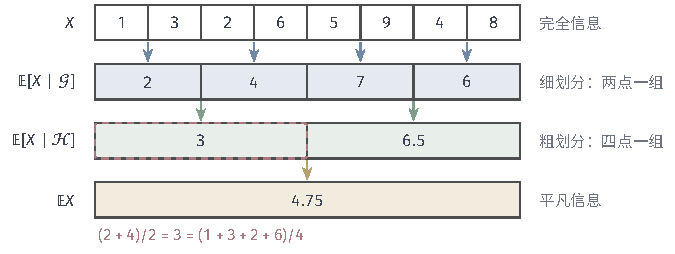
\includegraphics[width=112mm]{figures/02-abstract-mathematics/02-probability-spaces/tikz/cond-tower-layers/figure.pdf}
  \caption{塔式法则的逐层平均。八个样本点等概率，第一行是$X$的取值；第二行按相邻两点分组（信息$\mathcal G$），第三行按前后四点分组（信息$\mathcal H\subseteq\mathcal G$），第四行为平凡信息下的$\mathbb EX$。箭头表示在下一层的组内平均上一层；红色虚线框标出第一个粗组，图下方的红色算式说明在该组内先细后粗与直接粗分组的结果相同。}
  \label{fig:cond-tower-layers}
\end{figure}

两个没有包含关系的$\sigma$代数不能直接套用塔式法则。
在示例~\ref{ex:cond-four-points}的四点空间上，令$\mathcal G_1$由$\{0,2\},\{4,6\}$生成，$\mathcal G_2$由$\{0\},\{2,4,6\}$生成。
$\mathbb E[X\mid\mathcal G_1]$在四点上取$1,1,5,5$，$\mathbb E[X\mid\mathcal G_2]$取$0,4,4,4$。
再交换条件化：$\mathbb E\bigl[\mathbb E[X\mid\mathcal G_1]\bigm|\mathcal G_2\bigr]$取$1,\frac{11}{3},\frac{11}{3},\frac{11}{3}$，$\mathbb E\bigl[\mathbb E[X\mid\mathcal G_2]\bigm|\mathcal G_1\bigr]$取$2,2,4,4$。
两种顺序结果不同，而$\mathcal G_1\cap\mathcal G_2$是平凡$\sigma$代数，对它的条件期望是常数$3$，与两者都不相同。

\subsection{条件平均与误差控制}

\paragraph{条件Jensen不等式}
第~\ref{chap:probability-models}章的Jensen不等式（定理~\ref{thm:pmod-jensen}）说，对凸函数$\varphi$，先平均再作用不超过先作用再平均：$\varphi(\mathbb EX)\leq\mathbb E\varphi(X)$。
在每个组内做同样的比较，就得到它的条件版本。

\begin{theorem}[条件Jensen不等式]
\label{thm:cond-jensen}
设$\varphi:\mathbb R\to\mathbb R$是凸函数，$X$与$\varphi(X)$都可积。则
\[
  \varphi\bigl(\mathbb E[X\mid\mathcal G]\bigr)\leq\mathbb E[\varphi(X)\mid\mathcal G]\qquad\text{几乎必然}.
\]
\end{theorem}

\begin{proof}
凸函数在每点有有限的右导数$\varphi'_+(q)$，并且直线$\ell_q(x)=\varphi(q)+\varphi'_+(q)(x-q)$处处位于$\varphi$下方。
我们断言$\varphi(x)=\sup_{q\in\mathbb Q}\ell_q(x)$对每个$x$成立。
“$\geq$”由支撑性质得到；对“$\leq$”，取有理数$q_k\to x$，凸函数连续且右导数在$x$附近有界，所以$\ell_{q_k}(x)=\varphi(q_k)+\varphi'_+(q_k)(x-q_k)\to\varphi(x)$。
对每个有理数$q$，由$\ell_q(X)\leq\varphi(X)$以及定理~\ref{thm:cond-rules}的线性与保序，
\[
  \ell_q\bigl(\mathbb E[X\mid\mathcal G]\bigr)=\varphi(q)+\varphi'_+(q)\bigl(\mathbb E[X\mid\mathcal G]-q\bigr)\leq\mathbb E[\varphi(X)\mid\mathcal G]
\]
在某个零概率事件$N_q$之外成立。可数个零概率事件的并$N=\bigcup_{q\in\mathbb Q}N_q$仍是零概率事件，在$N$之外对全部有理数$q$同时取上确界即得结论。
\end{proof}

证明中把凸函数写成\emph{可数}条支撑直线的上确界，这一步不可省略：每条直线对应的不等式各有一个例外零集，只有可数多个才能合并。

图~\ref{fig:cond-jensen}在示例~\ref{ex:cond-four-points}的两组上取$\varphi(x)=x^2$。
第一组的条件平均是$1$，$\varphi(1)=1$；组内$\varphi$值的平均是$\frac{0+4}{2}=2$。
第二组分别是$25$与$26$。
两组中方块都落在圆点上方，差值都等于组内方差$1$；虚线弦的中点高于曲线，就是凸性在组内的表现。

\begin{figure}[htbp]
  \centering
  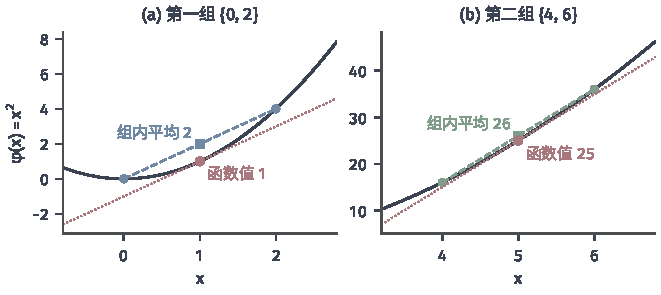
\includegraphics[width=112mm]{figures/02-abstract-mathematics/02-probability-spaces/matplotlib/cond-jensen/figure.pdf}
  \caption{条件Jensen不等式在四点空间两组上的表现，$\varphi(x)=x^2$。黑色曲线为$\varphi$，同色圆点为组内两点$(x,\varphi(x))$，虚线为连接它们的弦，方块为弦的中点即组内$\varphi$值的平均，红色圆点为条件平均处的函数值，红色点线为该处的支撑直线。(a)第一组$\{0,2\}$；(b)第二组$\{4,6\}$。}
  \label{fig:cond-jensen}
\end{figure}

\paragraph{矩收缩与平均误差的收缩}
取$\varphi(x)=|x|^p$（$p\geq1$）得到下面的推论，它说明条件平均不会放大矩，也不会放大两个变量之间的平均误差。

\begin{theorem}[推论：条件期望的收缩]
\label{thm:cond-contraction}
设$p\geq1$且$\mathbb E|X|^p<\infty$。则$|\mathbb E[X\mid\mathcal G]|^p\leq\mathbb E[|X|^p\mid\mathcal G]$几乎必然成立，从而
\[
  \mathbb E\bigl|\mathbb E[X\mid\mathcal G]\bigr|^p\leq\mathbb E|X|^p.
\]
特别地，对可积的$X,X'$，
\begin{equation}
  \mathbb E\bigl|\mathbb E[X\mid\mathcal G]-\mathbb E[X'\mid\mathcal G]\bigr|=\mathbb E\bigl|\mathbb E[X-X'\mid\mathcal G]\bigr|\leq\mathbb E|X-X'|.
  \label{eq:cond-l1-contraction}
\end{equation}
\end{theorem}

\begin{proof}
由$p\geq1$与$\mathbb E|X|^p<\infty$，第~\ref{chap:probability-models}章的矩单调性（定理~\ref{thm:pmod-moment-monotone}）给出$\mathbb E|X|<\infty$，于是$X$与$\varphi(X)=|X|^p$都可积。
$\varphi$是凸函数，由定理~\ref{thm:cond-jensen}得第一式；两边取期望并用全期望公式得第二式。
式~\eqref{eq:cond-l1-contraction}中的等号来自线性，不等号是$p=1$时对$X-X'$应用第二式。
\end{proof}

式~\eqref{eq:cond-l1-contraction}说，若$X_n$在平均绝对误差意义下接近$X$，那么在同一信息下取条件期望后仍然如此；第~\ref{chap:random-variable-convergence}章讨论平均收敛时会用到这个估计。

\paragraph{条件均方误差的分解}
现在把误差问题限定为：只依据$\mathcal G$中的信息给出一个预测$Z$，用均方误差$\mathbb E(X-Z)^2$衡量它离$X$多远。
候选预测是满足$\mathbb EZ^2<\infty$的$\mathcal G$可测随机变量，$X$也假设平方可积。
直观上，条件平均已经用尽了$\mathcal G$中的信息，其他预测与它的差距只会增加误差。

\begin{theorem}[条件均方误差最小]
\label{thm:cond-mse}
设$\mathbb EX^2<\infty$，$M=\mathbb E[X\mid\mathcal G]$。则$\mathbb EM^2\leq\mathbb EX^2$，并且对每个满足$\mathbb EZ^2<\infty$的$\mathcal G$可测随机变量$Z$，
\begin{equation}
  \mathbb E(X-Z)^2=\mathbb E(X-M)^2+\mathbb E(M-Z)^2.
  \label{eq:cond-mse-decomposition}
\end{equation}
因此$M$在这类预测中使均方误差最小，而且最小值只在$Z=M$几乎必然成立时达到。
\end{theorem}

\begin{proof}
$\mathbb EM^2\leq\mathbb EX^2$是定理~\ref{thm:cond-contraction}取$p=2$的情形。
把$X-Z$写成$(X-M)+(M-Z)$并展开平方，只需证明交叉项$\mathbb E[(X-M)(M-Z)]=0$。
令$H=M-Z$，它对$\mathcal G$可测且平方可积。由Cauchy--Schwarz不等式（定理~\ref{thm:pmod-cauchy-schwarz}），$HX$与$HM$都可积。
对$HX$用定理~\ref{thm:cond-pull-out}与全期望公式，
\[
  \mathbb E[HX]=\mathbb E\bigl[\mathbb E[HX\mid\mathcal G]\bigr]=\mathbb E[HM],
\]
即$\mathbb E[H(X-M)]=0$。于是式~\eqref{eq:cond-mse-decomposition}成立。
等式右边第二项非负，且为零当且仅当$Z=M$几乎必然成立，由此得到最小性与唯一性。
\end{proof}

式~\eqref{eq:cond-mse-decomposition}把任一预测的误差拆成两部分：$\mathbb E(X-M)^2$是只用$\mathcal G$时无论如何都消除不了的误差，$\mathbb E(M-Z)^2$是预测偏离条件平均的代价。
取平凡信息，$M=\mathbb EX$，分解就是熟悉的$\mathbb E(X-c)^2=\operatorname{Var}X+(\mathbb EX-c)^2$。
这里只用了展开平方和交叉项为零这一个恒等式；把条件期望看成函数空间中的正交投影，是第~\ref{part:function-spaces}部分的内容。

图~\ref{fig:cond-mse-decomposition}在示例~\ref{ex:cond-square-noise}的模型中（$\sigma^2=0.25$）比较四个只依赖$Y$的预测。
蓝色部分对四个预测都是$\mathbb E(X-M)^2=\mathbb E\varepsilon^2=0.25$；黄色部分是$\mathbb E(M-Z)^2$，常数预测$Z=1$为$\operatorname{Var}(Y^2)=2$，$Z=|Y|$为$\mathbb E(Y^2-|Y|)^2=4-4\sqrt{2/\pi}\approx0.808$，$Z=0.8Y^2$为$0.04\,\mathbb EY^4=0.12$。
菱形是用$400000$个模拟样本算出的均方误差，与两部分之和吻合。
蓝色底座的高度不随预测改变，这就是“无论怎样利用$Y$都消除不了的误差”。

\begin{figure}[htbp]
  \centering
  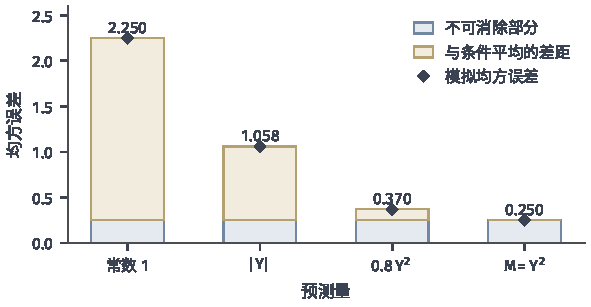
\includegraphics[width=100mm]{figures/02-abstract-mathematics/02-probability-spaces/matplotlib/cond-mse-decomposition/figure.pdf}
  \caption{条件均方误差分解~\eqref{eq:cond-mse-decomposition}的数值对照。模型为$Y\sim N(0,1)$，$\varepsilon\sim N(0,0.25)$与$Y$独立，$X=Y^2+\varepsilon$，$M=\mathbb E[X\mid Y]=Y^2$。每根柱子对应一个$\sigma(Y)$可测预测$Z$：蓝色为$\mathbb E(X-M)^2=0.25$，黄色为精确计算的$\mathbb E(M-Z)^2$，柱顶数字为二者之和；菱形为固定随机种子下$400000$个样本的经验均方误差。}
  \label{fig:cond-mse-decomposition}
\end{figure}

\subsection{固定信息下的条件极限}

\paragraph{取无穷值的条件期望}
交换条件期望与极限时，常常遇到不一定可积的非负随机变量，例如单调上升列的极限。
为此先把条件期望推广到非负随机变量，允许它取$+\infty$。

设$X\geq0$。截断$X\wedge n=\min(X,n)$有界，因而可积；由保序性，$Z_n=\mathbb E[X\wedge n\mid\mathcal G]$几乎必然单调不减；在单调性失效的那个零概率事件（它属于$\mathcal G$）上，把各$Z_n$都改为$0$，这只换了版本，此后可设$Z_n$处处单调不减。
定义
\[
  \mathbb E[X\mid\mathcal G]=\lim_{n\to\infty}\mathbb E[X\wedge n\mid\mathcal G],
\]
它是取值于$[0,\infty]$的$\mathcal G$可测随机变量。
对每个$A\in\mathcal G$，两边分别用单调收敛定理，
\[
  \mathbb E\bigl[\mathbb E[X\mid\mathcal G]\mathbb I_A\bigr]=\lim_n\mathbb E[Z_n\mathbb I_A]=\lim_n\mathbb E[(X\wedge n)\mathbb I_A]=\mathbb E[X\mathbb I_A],
\]
所以积分刻画~\eqref{eq:cond-defining-identity}照样成立，两边允许同为$+\infty$。

这一推广仍然几乎必然唯一。
若$Z,Z'$都是取值于$[0,\infty]$的$\mathcal G$可测随机变量，且对每个$A\in\mathcal G$满足$\mathbb E[Z\mathbb I_A]=\mathbb E[Z'\mathbb I_A]=\mathbb E[X\mathbb I_A]$，令$A_k=\{Z<Z',\,Z\leq k\}\in\mathcal G$。
则$\mathbb E[Z'\mathbb I_{A_k}]=\mathbb E[Z\mathbb I_{A_k}]\leq k$，所以$Z'$在$A_k$上几乎必然有限，$(Z'-Z)\mathbb I_{A_k}$非负且积分为零，得$\mathbb P(A_k)=0$。
对$k$取可数并得$\mathbb P(Z<Z')=0$，对称地得$\mathbb P(Z'<Z)=0$。
当$X$本身可积时，这一定义与定义~\ref{def:cond-expectation}一致。

\paragraph{条件单调收敛与条件Fatou}
有了非负情形的定义，普通积分中的单调收敛定理与Fatou引理都有固定信息下的版本。

\begin{theorem}[条件单调收敛定理与条件Fatou引理]
\label{thm:cond-monotone}
固定子$\sigma$代数$\mathcal G$。
\begin{enumerate}
  \item 若$0\leq X_n\uparrow X$几乎必然成立，则$\mathbb E[X_n\mid\mathcal G]\uparrow\mathbb E[X\mid\mathcal G]$几乎必然成立。
  \item 若$X_n\geq0$，则$\mathbb E[\liminf_nX_n\mid\mathcal G]\leq\liminf_n\mathbb E[X_n\mid\mathcal G]$几乎必然成立。
\end{enumerate}
其中的条件期望均按上一段取值于$[0,\infty]$。
\end{theorem}

\begin{proof}
(1) 对每个截断水平$k$，$X_n\wedge k\leq X_{n+1}\wedge k$，由保序性与极限定义，$Z_n=\mathbb E[X_n\mid\mathcal G]$几乎必然单调不减。令$Z=\lim_nZ_n$，它对$\mathcal G$可测。对每个$A\in\mathcal G$，两次使用单调收敛定理，
\[
  \mathbb E[Z\mathbb I_A]=\lim_n\mathbb E[Z_n\mathbb I_A]=\lim_n\mathbb E[X_n\mathbb I_A]=\mathbb E[X\mathbb I_A].
\]
由上一段的唯一性，$Z=\mathbb E[X\mid\mathcal G]$。

(2) 令$Y_n=\inf_{k\geq n}X_k$，则$0\leq Y_n\uparrow\liminf_kX_k$。对每个$k\geq n$，$Y_n\leq X_k$，由保序性$\mathbb E[Y_n\mid\mathcal G]\leq\mathbb E[X_k\mid\mathcal G]$；可数个$k$的例外零集合并后，得$\mathbb E[Y_n\mid\mathcal G]\leq\inf_{k\geq n}\mathbb E[X_k\mid\mathcal G]$。由(1)令$n\to\infty$，左边上升到$\mathbb E[\liminf_kX_k\mid\mathcal G]$，右边上升到$\liminf_k\mathbb E[X_k\mid\mathcal G]$。
\end{proof}

\paragraph{条件控制收敛}
最常用的是控制收敛的条件版本。
它的证明思路是把“误差趋于零”改写成一个单调上升列，再借助条件单调收敛；减法步骤需要控制变量的条件期望有限。

\begin{theorem}[条件控制收敛定理]
\label{thm:cond-dominated}
设$X_n\to X$几乎必然成立，并存在可积随机变量$Y$，使$|X_n|\leq Y$对每个$n$几乎必然成立。则
\[
  \mathbb E\bigl[|X_n-X|\bigm|\mathcal G\bigr]\to0,\qquad
  \mathbb E[X_n\mid\mathcal G]\to\mathbb E[X\mid\mathcal G]\qquad\text{几乎必然}.
\]
\end{theorem}

\begin{proof}
由$|X_n|\leq Y$与$X_n\to X$得$|X|\leq Y$，所以$X$可积。
令$U_n=\sup_{k\geq n}|X_k-X|$，则$U_n\downarrow0$且$0\leq U_n\leq2Y$几乎必然成立。
于是$0\leq2Y-U_n\uparrow2Y$，由定理~\ref{thm:cond-monotone}，
\[
  \mathbb E[2Y-U_n\mid\mathcal G]\uparrow\mathbb E[2Y\mid\mathcal G]\qquad\text{几乎必然}.
\]
$Y$与$U_n$都可积，$\mathbb E[Y\mid\mathcal G]$几乎必然有限，所以可以用线性把左边写成$2\mathbb E[Y\mid\mathcal G]-\mathbb E[U_n\mid\mathcal G]$，两边减去有限的$2\mathbb E[Y\mid\mathcal G]$，得$\mathbb E[U_n\mid\mathcal G]\downarrow0$。
由保序性，$\mathbb E[|X_n-X|\mid\mathcal G]\leq\mathbb E[U_n\mid\mathcal G]$，第一式得证；再由定理~\ref{thm:cond-rules}的绝对值规则，
\[
  \bigl|\mathbb E[X_n\mid\mathcal G]-\mathbb E[X\mid\mathcal G]\bigr|\leq\mathbb E\bigl[|X_n-X|\bigm|\mathcal G\bigr],
\]
第二式得证。
\end{proof}

证明中“减去有限的$2\mathbb E[Y\mid\mathcal G]$”一步说明了控制变量可积的作用：若条件期望可以取$+\infty$，就会出现$\infty-\infty$。
没有控制时结论可以失败。
取平凡信息，$\Omega=(0,1)$上$X_n=n\mathbb I_{(0,1/n)}$几乎处处趋于$0$，但$\mathbb E[X_n\mid\mathcal G]=\mathbb EX_n=1$不趋于$0$；第~\ref{chap:random-variable-convergence}章示例~\ref{ex:conv-spike}会从平均误差的角度重新分析这个例子。

本小节的所有陈述都固定同一个$\mathcal G$。
依概率收敛、一致可积与平均收敛之间的关系属于第~\ref{chap:random-variable-convergence}章；信息本身随时间增加时条件期望的极限，例如鞅收敛，属于\BookPartRef{part:dynamical-systems-control-decision-and-games}{卷三“过程与轨迹演化”部分}。

\section{概率核}
\label{sec:cond-kernels}

条件期望逐个处理可积变量；条件分布则要求对每个观测值同时给出一整个概率分布，并且这些分布随观测值可测地变化。
描述这种“输入一个状态，输出一个概率分布”的对象就是概率核。
本节先独立建立概率核、核积分、由核构造联合分布以及核的复合，下一节再用它准确表述条件分布。
这里只处理概率核：上一部分在测度层面讨论了推前与密度，概率核把确定的映射推广为随机的输出，所需的可测性与积分交换都在本节证明。

\subsection{概率核的定义}

\paragraph{有限集合上的随机矩阵}
先看有限的情形。
设输入状态集合$S=\{1,2,3\}$，输出状态集合$T=\{a,b,c\}$。
一张非负矩阵$K=(K(s,t))$，若每一行之和都是$1$，就称为随机矩阵；第$s$行是输入为$s$时输出的概率分布。
图~\ref{fig:cond-finite-kernel}给出一个例子：输入$2$以概率$0.2,0.6,0.2$分别输出$a,b,c$，三行之和都是$1$。
对输出集合$B\subseteq T$，记$K(s,B)=\sum_{t\in B}K(s,t)$，它是输入为$s$时输出落入$B$的概率。

\begin{figure}[htbp]
  \centering
  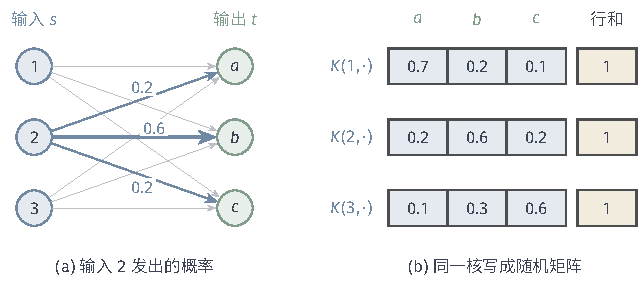
\includegraphics[width=108mm]{figures/02-abstract-mathematics/02-probability-spaces/tikz/cond-finite-kernel/figure.pdf}
  \caption{有限随机矩阵作为概率核。输入$S=\{1,2,3\}$，输出$T=\{a,b,c\}$。(a)以输入$2$为例，蓝色箭头上的数是它输出各状态的概率，灰线表示其余输入的转移；(b)同一核写成随机矩阵，第$s$行是分布$K(s,\cdot)$，右侧黄色格为行和$1$。}
  \label{fig:cond-finite-kernel}
\end{figure}

\paragraph{一般可测空间上的概率核}
在一般空间中，输入可以有不可数多个，输出的“行”也不再是有限向量。
随机矩阵的两项性质需要分别推广：固定输入时，输出端必须是一个概率测度；固定输出事件时，它的概率随输入的变化必须可测，否则无法再对输入求平均。

\begin{definition}[概率核]
\label{def:cond-kernel}
设$(S,\mathcal S)$与$(T,\mathcal T)$是可测空间。映射$K:S\times\mathcal T\to[0,1]$若满足
\begin{enumerate}
  \item 对每个$s\in S$，$K(s,\cdot)$是$(T,\mathcal T)$上的概率测度；
  \item 对每个$B\in\mathcal T$，$s\mapsto K(s,B)$是$\mathcal S$可测函数，
\end{enumerate}
则称$K$为从$S$到$T$的\term{概率核}（probability kernel）。
\end{definition}

它就是总质量为$1$的测度核。
第一项保证每个输入给出合法的输出分布，第二项保证当输入本身随机时，$\mathbb P(\text{输出}\in B)$可以通过对输入积分来计算。
有限情形中第二项自动成立，因为有限集合上（取全部子集为可测集时）的每个函数都可测。

\paragraph{确定性核与密度核}
两类常见的核位于两个极端。
设$f:S\to T$可测，令
\[
  K(s,B)=\mathbb I_B(f(s)),
\]
即输入$s$时以概率$1$输出$f(s)$。固定$s$时$K(s,\cdot)$是单点质量；固定$B$时$s\mapsto\mathbb I_B(f(s))=\mathbb I_{f^{-1}(B)}(s)$可测，正是因为$f$可测。
这称为\term{确定性核}（deterministic kernel），可测映射因此可以看成没有随机性的核。

另一端是密度核。
设$\lambda$是$(T,\mathcal T)$上的$\sigma$有限测度，$k:S\times T\to[0,\infty)$对$\mathcal S\otimes\mathcal T$可测，并且对每个$s$有$\int_Tk(s,t)\,\lambda(dt)=1$。令
\[
  K(s,B)=\int_Bk(s,t)\,\lambda(dt).
\]
固定$s$时，这是密度为$k(s,\cdot)$的概率测度；固定$B$时，$s\mapsto K(s,B)$的可测性来自一般的Tonelli定理（第~\ref{sec:integral-tonelli}节），这也是要求$k$关于输入与输出\emph{联合}可测的原因。

图~\ref{fig:cond-kernel-types}把两类核的“行”画在一起，取$f(s)=s$。
左图中每个输入$s$只在$t=s$处放一个点质量；右图中每个输入给出以$s$为中心、标准差$0.15$的正态密度。
密度核的所有行都关于同一个Lebesgue测度有密度；确定性核的各行却没有共同的$\sigma$有限参考测度。
事实上，若$\sigma$有限测度$\lambda$使每个单点质量$\delta_s$（$s\in\mathbb R$）都关于$\lambda$绝对连续，则每个$\lambda(\{s\})>0$；但$\sigma$有限测度至多有可数个正质量的单点（每个有限质量的块中，质量超过$1/m$的单点至多有限个），矛盾。
所以概率核比“条件密度”适用得更广：没有共同参考密度时，核仍然存在。

\begin{figure}[htbp]
  \centering
  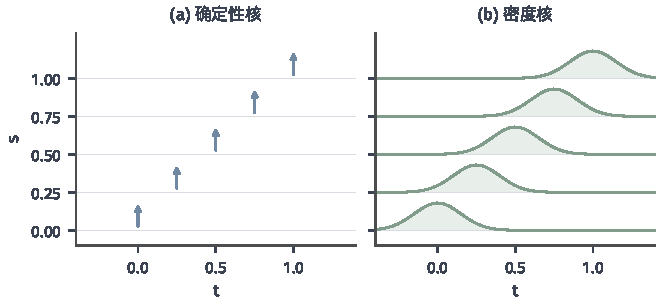
\includegraphics[width=112mm]{figures/02-abstract-mathematics/02-probability-spaces/matplotlib/cond-kernel-types/figure.pdf}
  \caption{两类概率核的行$K(s,\cdot)$，横轴为输出$t$，每条水平基线对应一个输入$s\in\{0,0.25,0.5,0.75,1\}$。(a)确定性核$K(s,\cdot)=\delta_{f(s)}$，$f(s)=s$，箭头表示单点质量；(b)密度核，$K(s,dt)$为$N(s,0.15^2)$，为便于比较，各密度曲线缩放到相同峰高。}
  \label{fig:cond-kernel-types}
\end{figure}

\subsection{核积分与联合分布}

\paragraph{核积分}
给定输入$s$后，对输出的函数$f$求平均，得到
\begin{equation}
  Kf(s)=\int_Tf(t)\,K(s,dt),
  \label{eq:cond-kernel-integral}
\end{equation}
这里$f$是非负可测函数（允许$Kf$取$+\infty$）或有界可测函数。
在有限情形，$Kf$就是随机矩阵乘以列向量$f$。

$Kf$作为输入的函数是可测的，证明沿积分的标准构造逐步进行。
若$f=\mathbb I_B$，则$Kf(s)=K(s,B)$，由核的第二项条件可测；对非负简单函数，$Kf$是可测函数的线性组合。
对非负可测$f$，取非负简单函数$f_n\uparrow f$，对每个固定的$s$用单调收敛定理得$Kf_n(s)\uparrow Kf(s)$，可测函数列的逐点极限仍可测。
对有界$f$，分别处理$f^+$与$f^-$，两者的核积分都有限。

\paragraph{输出分布}
若输入本身随机，服从$(S,\mathcal S)$上的概率分布$\mu$，那么输出落入$B$的总概率应当是各输入下概率的加权平均：
\[
  \mu K(B)=\int_SK(s,B)\,\mu(ds),\qquad B\in\mathcal T.
\]
由核的第二项条件，右边的被积函数可测。$\mu K(T)=1$；若$B_1,B_2,\ldots$两两不交，则$K(s,\bigcup_kB_k)=\sum_kK(s,B_k)$，对非负部分和用单调收敛定理得可数可加性。
所以$\mu K$是$(T,\mathcal T)$上的概率测度，称为输出分布。
同样从示性函数出发逐步推广，可得$\int_Tf\,d(\mu K)=\int_SKf\,d\mu$对非负或有界可测$f$成立。

在有限情形，$\mu K$就是行向量$\mu$乘随机矩阵$K$。
取$\mu=(0.5,0.3,0.2)$，图~\ref{fig:cond-finite-kernel}的核给出
\[
  \begin{aligned}
  \mu K&=0.5\,(0.7,0.2,0.1)+0.3\,(0.2,0.6,0.2)+0.2\,(0.1,0.3,0.6)\\
  &=(0.43,0.34,0.23).
  \end{aligned}
\]
输入的不确定性就这样按行加权传到输出。

\paragraph{由输入分布与核构造联合分布}
输出分布只记录了输出，丢掉了输入与输出的配对。
有限情形中，配对$(s,t)$的概率是$\mu(s)K(s,t)$，把它排成一张表，按列求和得到$\mu K$，按行求和得到$\mu$，如图~\ref{fig:cond-joint-from-kernel}所示。
一般情形下，我们希望对乘积空间中的集合$A$令
\[
  M(A)=\int_SK(s,A_s)\,\mu(ds),\qquad A_s=\{t\in T:(s,t)\in A\},
\]
即先固定输入$s$，用$K(s,\cdot)$度量$A$在$s$处的截面，再对$s$平均。
这需要先确认截面可测，并且$s\mapsto K(s,A_s)$可测。

\begin{figure}[htbp]
  \centering
  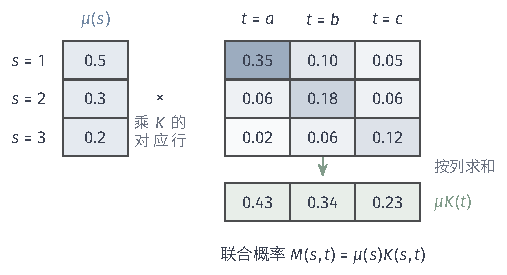
\includegraphics[width=86mm]{figures/02-abstract-mathematics/02-probability-spaces/tikz/cond-joint-from-kernel/figure.pdf}
  \caption{由输入分布与核构造联合分布。输入分布$\mu=(0.5,0.3,0.2)$，核$K$同图~\ref{fig:cond-finite-kernel}；中间表格的第$s$行是$\mu(s)$乘$K$的第$s$行，底色深浅与概率成正比；按列求和得到输出分布$\mu K=(0.43,0.34,0.23)$，按行求和则回到$\mu$。}
  \label{fig:cond-joint-from-kernel}
\end{figure}

\begin{theorem}[由输入分布与核构造联合分布]
\label{thm:cond-kernel-joint}
设$\mu$是$(S,\mathcal S)$上的概率测度，$K$是从$S$到$T$的概率核。则：
\begin{enumerate}
  \item 对每个$A\in\mathcal S\otimes\mathcal T$，截面$A_s\in\mathcal T$，且$s\mapsto K(s,A_s)$对$\mathcal S$可测；
  \item $M(A)=\int_SK(s,A_s)\,\mu(ds)$是$\mathcal S\otimes\mathcal T$上的概率测度，它是满足$M(B\times C)=\int_BK(s,C)\,\mu(ds)$（$B\in\mathcal S$，$C\in\mathcal T$）的唯一概率测度；
  \item 对非负的$\mathcal S\otimes\mathcal T$可测函数$f$，$s\mapsto\int_Tf(s,t)\,K(s,dt)$对$\mathcal S$可测，并且
  \begin{equation}
    \int_{S\times T}f\,dM=\int_S\Bigl(\int_Tf(s,t)\,K(s,dt)\Bigr)\mu(ds);
    \label{eq:cond-kernel-iterated}
  \end{equation}
  若$f$有符号且$\int|f|\,dM<\infty$，内层积分对$\mu$几乎每个$s$有限，式~\eqref{eq:cond-kernel-iterated}仍然成立。
\end{enumerate}
$M$的第一边缘是$\mu$，第二边缘是$\mu K$。
\end{theorem}

\begin{proof}
(1) 令$\mathcal D$为满足以下条件的$A\in\mathcal S\otimes\mathcal T$组成的族：每个截面$A_s\in\mathcal T$，且$s\mapsto K(s,A_s)$可测。
对可测矩形$B\times C$，截面在$s\in B$时为$C$，否则为空集，所以$K(s,(B\times C)_s)=\mathbb I_B(s)K(s,C)$可测，矩形属于$\mathcal D$。
若$A\in\mathcal D$，则$(A^c)_s=(A_s)^c$，$K(s,(A^c)_s)=1-K(s,A_s)$可测；若$A_1,A_2,\ldots\in\mathcal D$两两不交，则各截面两两不交，$K(s,(\bigcup_kA_k)_s)=\sum_kK(s,(A_k)_s)$是可测函数的级数和。
所以$\mathcal D$对补集与不交可数并封闭。可测矩形构成包含$S\times T$的$\pi$系统并生成$\mathcal S\otimes\mathcal T$，由$\pi$--$\lambda$定理，$\mathcal D=\mathcal S\otimes\mathcal T$。

(2) 由(1)，$M$有定义，且$M(S\times T)=1$。若$A_k$两两不交，对$K(s,(\bigcup_kA_k)_s)=\sum_kK(s,(A_k)_s)$用单调收敛定理得$M(\bigcup_kA_k)=\sum_kM(A_k)$。矩形公式就是(1)中的计算。两个在矩形上取值相同的概率测度，由定理~\ref{thm:measure-uniqueness}在整个乘积$\sigma$代数上相等。

(3) 对$f=\mathbb I_A$，内层积分为$K(s,A_s)$，式~\eqref{eq:cond-kernel-iterated}就是$M$的定义。由线性推广到非负简单函数；对一般非负$f$，取非负简单函数$f_n\uparrow f$，内层对每个$s$用单调收敛定理，外层再用一次，可测性与等式都保留。
对绝对可积的$f$，对$|f|$用非负情形知内层积分$\int|f(s,t)|K(s,dt)$对$\mu$几乎每个$s$有限；在这些$s$上把$f=f^+-f^-$的两部分分别代入并相减即可。

取$A=B\times T$与$A=S\times C$，分别得$M(B\times T)=\mu(B)$与$M(S\times C)=\mu K(C)$。
\end{proof}

我们把这个联合分布记作$\mu(ds)K(s,dt)$，或简记为$\mu\otimes K$。
当$K(s,\cdot)=\nu$不依赖$s$时，它就是乘积测度$\mu\otimes\nu$，联合分布中输入与输出独立；一般的核则让输出分布随输入改变，从而在联合分布中建立依赖。
本节从输入分布和核出发得到联合分布；下一节研究反方向的问题：给定联合分布，怎样恢复以一个坐标为输入的条件核。

\subsection{概率核的复合}

\paragraph{先平均中间状态}
设$K$是从$S$到$T$的概率核，$L$是从$T$到$U$的概率核。
输入$s$先经$K$得到中间状态$t$，再经$L$得到输出$u$；我们只关心从$s$到$u$的规律，因此对中间状态求平均：
\[
  (KL)(s,C)=\int_TL(t,C)\,K(s,dt),\qquad s\in S,\ C\in\mathcal U.
\]
用核积分的记号，$(KL)(s,C)=K\bigl(L(\cdot,C)\bigr)(s)$。

\begin{lemma}[核的复合与结合律]
\label{lem:cond-kernel-composition}
$KL$是从$S$到$U$的概率核，并且对非负可测$g$有$(KL)g=K(Lg)$。若再给定从$U$到$V$的概率核$N$，则$(KL)N=K(LN)$。
\end{lemma}

\begin{proof}
固定$C$，$t\mapsto L(t,C)$是取值于$[0,1]$的可测函数，由核积分的可测性，$s\mapsto(KL)(s,C)$可测。
固定$s$，$(KL)(s,U)=1$；若$C_k$两两不交，$L(t,\bigcup_kC_k)=\sum_kL(t,C_k)$，对$K(s,dt)$积分并用单调收敛定理得可数可加性。所以$KL$是概率核。
等式$(KL)g=K(Lg)$对$g=\mathbb I_C$就是定义；由线性推广到非负简单函数，再在两边逐层用单调收敛定理推广到非负可测$g$。
最后，对$D\in\mathcal V$，令$g=N(\cdot,D)$，则$((KL)N)(s,D)=(KL)g(s)=K(Lg)(s)=(K(LN))(s,D)$。
\end{proof}

在有限集合上，$(KL)(s,u)=\sum_tK(s,t)L(t,u)$，复合就是随机矩阵的乘法，结合律就是矩阵乘法的结合律。
同样可以验证$\mu(KL)=(\mu K)L$：先把输入分布推到中间，再推到输出，与直接用复合核推送结果相同。

\paragraph{两个翻转核}
取$S=T=U=\{0,1\}$。
第一个核以概率$p$翻转比特、以概率$1-p$保持不变，第二个核的翻转概率为$q$。
从输入$0$到输出$1$有两条路径：先保持再翻转，概率$(1-p)q$；先翻转再保持，概率$p(1-q)$。
对中间状态求和，复合核的翻转概率为
\[
  (KL)(0,\{1\})=p(1-q)+(1-p)q.
\]
取$p=0.1$，$q=0.2$，得$0.08+0.18=0.26$，如图~\ref{fig:cond-kernel-composition}所示。
复合后仍是一个翻转核，并且满足$1-2\times0.26=0.48=(1-2p)(1-2q)$：用$\pm1$编码比特时，$1-2p$是输出与输入乘积的平均，经过两次翻转，这一乘积平均相乘。

\begin{figure*}[htbp]
  \centering
  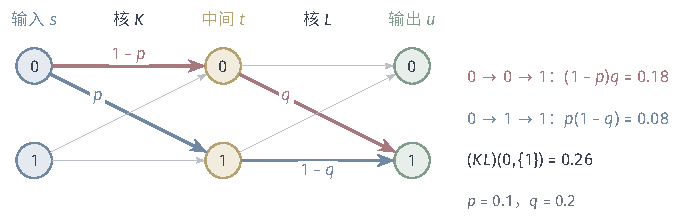
\includegraphics[width=115mm]{figures/02-abstract-mathematics/02-probability-spaces/tikz/cond-kernel-composition/figure.pdf}
  \caption{两个二元翻转核的复合。核$K$的翻转概率为$p=0.1$，核$L$的翻转概率为$q=0.2$。从输入$0$到输出$1$的两条路径分别用红色（$0\to0\to1$）与蓝色（$0\to1\to1$）标出，灰线为其余转移；两条路径的概率相加得到复合核的翻转概率$0.26$。}
  \label{fig:cond-kernel-composition}
\end{figure*}

本节只处理有限个核的复合以及由一个核构造联合分布。
沿时间不断复合核得到的过程模型、Markov性，以及无限序列上联合分布的存在性，与上一节提到的鞅收敛一样，都留给卷三的过程部分。

\section{条件分布}
\label{sec:cond-distributions}

有了概率核的语言，我们可以把逐个事件的条件概率组织成一个整体对象。
本节依次回答四个问题：这个对象怎样定义，何时存在、在什么意义下唯一，怎样用它计算条件平均，以及有密度时怎样具体写出它。

\subsection{条件分布的定义}

\paragraph{从逐事件条件概率到一个核}
设$X$是取值于可测空间$(E,\mathcal E)$的随机对象，$\mathcal G\subseteq\mathcal F$是子$\sigma$代数。
对每个$B\in\mathcal E$，第~\ref{sec:cond-definition}节给出条件概率$\mathbb P(X\in B\mid\mathcal G)$，但它只是一个几乎必然确定的版本。
我们希望一次选好所有版本，使它们在每个样本点处共同构成$E$上的一个概率分布。

\begin{definition}[正则条件分布]
\label{def:cond-regular-distribution}
设$X$取值于$(E,\mathcal E)$，$\mathcal G\subseteq\mathcal F$是子$\sigma$代数。
若$K_{\mathcal G}$是从$(\Omega,\mathcal G)$到$(E,\mathcal E)$的概率核，并且对每个$B\in\mathcal E$，
\[
  K_{\mathcal G}(\cdot,B)=\mathbb P(X\in B\mid\mathcal G)\qquad\text{几乎必然},
\]
即$K_{\mathcal G}(\cdot,B)$是条件概率$\mathbb P(X\in B\mid\mathcal G)$的一个版本，则称$K_{\mathcal G}$为$X$给定$\mathcal G$的\term{正则条件分布}（regular conditional distribution）。
\end{definition}

定义包含两项不同的要求。
第一项是逐事件的：每个$K_{\mathcal G}(\cdot,B)$都对$\mathcal G$可测，并在$\mathcal G$的事件上保持概率。
第二项是整体的：对每个固定的$\omega$，$B\mapsto K_{\mathcal G}(\omega,B)$必须是概率测度。
逐事件的条件概率总是存在，但每个版本都可以在各自的零概率事件上任意改动；第二项要求所有这些改动在同一个$\omega$处相容，这并不自动成立。

\paragraph{以观测值为输入的条件核}
信息由观测$Y$给出时，我们更希望条件分布直接以观测值为输入。
设$Y$取值于$(D,\mathcal D)$。若$K$是从$D$到$E$的概率核，且对每个$B\in\mathcal E$，
\[
  K(Y,B)=\mathbb P(X\in B\mid Y)\qquad\text{几乎必然},
\]
就称$K$为$X$给定$Y$的条件分布（或条件核），并记
\[
  \mathbb P(X\in B\mid Y=y)=K(y,B).
\]
此时$\omega\mapsto K(Y(\omega),\cdot)$是$X$给定$\sigma(Y)$的正则条件分布：它对$\sigma(Y)$可测，因为$K(\cdot,B)$可测而$Y$可测。

由式~\eqref{eq:cond-given-y-identity}，上述要求等价于对每个$B\in\mathcal E$、$C\in\mathcal D$，
\begin{equation}
  \mathbb P(X\in B,\,Y\in C)=\int_CK(y,B)\,P_Y(dy).
  \label{eq:cond-kernel-disintegration}
\end{equation}
对照定理~\ref{thm:cond-kernel-joint}，这说明$(Y,X)$的联合分布正是$P_Y(dy)K(y,dx)$：两者在可测矩形上一致，由唯一性在整个乘积$\sigma$代数上一致。
所以条件核就是把联合分布按第一个坐标分解所得的核，即联合分布的一种核分解。

记号$\mathbb P(X\in B\mid Y=y)$来自条件核，而不是在$\mathbb P(Y=y)=0$时继续使用事件概率之比。
式~\eqref{eq:cond-kernel-disintegration}只对$y$积分，所以核在一个$P_Y$零集上的取值不受约束；条件核首先确定的是$P_Y$几乎处处意义下的条件规律。
例如$X=Y+\varepsilon$，其中$\varepsilon\sim N(0,1)$与$Y$独立，则$K(y,\cdot)=N(y,1)$满足式~\eqref{eq:cond-kernel-disintegration}，每个$\{Y=y\}$的概率是否为零都不影响这一说法。

\subsection{条件分布的存在性与版本}

\paragraph{实值情形：先在有理点上选版本}
为什么逐事件的条件概率不足以拼成分布？
$\mathcal E$中的事件通常有不可数多个，每个版本各带一个例外零集，不可数个零集的并可能不是零集，甚至不可测。
实值情形的出路是：分布由分布函数决定，而分布函数又由它在有理点上的值决定，于是只需在可数个点上选版本。

设$X$是实值随机变量。对每个有理数$r$，取$\mathbb P(X\leq r\mid\mathcal G)$的一个版本$G_r$。
下列三类性质对每个固定的有理数（或有理数对）几乎必然成立：
\begin{enumerate}
  \item 单调：$r<r'$时$G_r\leq G_{r'}$，由保序性得到；
  \item 有理点右连续：$G_{r+1/n}\to G_r$，因为$\mathbb I_{\{X\leq r+1/n\}}\downarrow\mathbb I_{\{X\leq r\}}$，由条件控制收敛定理~\ref{thm:cond-dominated}得到；
  \item 端点极限：整数$k\to-\infty$时$G_k\to0$，$k\to+\infty$时$G_k\to1$，同样由条件控制收敛得到。
\end{enumerate}
这些性质只涉及可数个有理数（或有理数对），各自的例外零集合并后，得到一个零概率事件$N\in\mathcal G$。

在$N$之外令
\[
  F(x,\omega)=\inf_{r\in\mathbb Q,\,r>x}G_r(\omega),\qquad x\in\mathbb R.
\]
它关于$x$单调不减、右连续，在$-\infty$与$+\infty$处的极限分别为$0$与$1$，因而是一个分布函数，唯一确定$\mathbb R$上的一个Borel概率测度$K_{\mathcal G}(\omega,\cdot)$。
在$N$上，令$K_{\mathcal G}(\omega,\cdot)$等于一个固定的概率测度，例如$N(0,1)$。
由有理点右连续与单调性，在$N$外$F(r,\omega)=G_r(\omega)$对每个有理数$r$成立。$G_r$只在有理点上选定，取$\inf_{r>x}$既把它延拓到全部实数，又保证延拓结果处处右连续，同时不改变有理点上已选好的值。

图~\ref{fig:cond-cdf-rationals}用一个有原子的例子展示这一构造。
设给定$Y=y$时$Z\sim N(y-0.5,0.25)$，$X=\max(Z,0)$，于是条件分布函数在$x<0$时为$0$，在$x\geq0$时为$\Phi\bigl((x-y+0.5)/0.5\bigr)$，在$0$处有跳跃。
左图中圆点是二进有理点上的值，曲线是由这些值右连续化得到的分布函数；右图取$y=0.5$，有理点$r=\frac12,\frac14,\frac18,\ldots$从右侧逼近$0$，函数值依次为$0.841,0.691,0.599,\ldots$，下确界$0.5$正是跳跃后的值$F(0\mid y)$。

\begin{figure}[htbp]
  \centering
  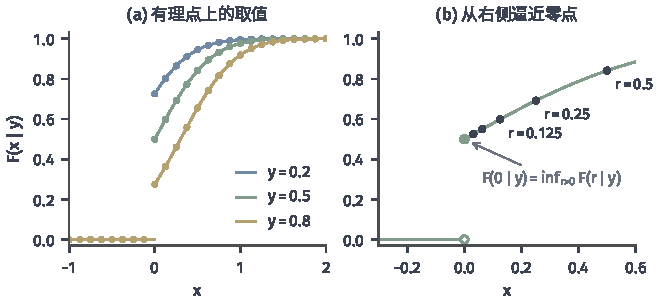
\includegraphics[width=112mm]{figures/02-abstract-mathematics/02-probability-spaces/matplotlib/cond-cdf-rationals/figure.pdf}
  \caption{由有理点上的值构造条件分布函数。模型为$X=\max(Z,0)$，给定$Y=y$时$Z\sim N(y-0.5,0.5^2)$，条件分布函数在$x=0$处跳跃$\Phi(1-2y)$。(a)$y=0.2,0.5,0.8$时，圆点为$x=k/8$（$k=-8,\ldots,16$）处的取值，曲线为右连续化后的分布函数；(b)$y=0.5$时，黑点为$r=2^{-1},\ldots,2^{-5}$处的取值，实心圆为$F(0\mid y)=0.5$，空心圆表示左极限$0$。}
  \label{fig:cond-cdf-rationals}
\end{figure}

\paragraph{标准Borel空间上的存在定理}
上面的构造用到了实数的两项结构：有理数是可数的稠密集，分布由分布函数决定。
对一般取值空间，相应的充分条件是\term{标准Borel空间}（standard Borel space）：与某个完备可分度量空间的Borel子集可测同构的可测空间。
实数、有限维欧氏空间及其Borel子集、可数离散空间都属于此类。

\begin{theorem}[正则条件分布的存在性]
\label{thm:cond-regular-existence}
\begin{enumerate}
  \item 设$X$是实值随机变量，或更一般地取值于标准Borel空间$(E,\mathcal E)$，$\mathcal G\subseteq\mathcal F$是任意子$\sigma$代数，则$X$给定$\mathcal G$的正则条件分布存在。
  \item 设$X$取值于标准Borel空间$(E,\mathcal E)$，$Y$取值于可测空间$(D,\mathcal D)$，则存在从$D$到$E$的概率核$K$，使$K(Y,B)=\mathbb P(X\in B\mid Y)$对每个$B\in\mathcal E$几乎必然成立。特别地，$X,Y$都取值于标准Borel空间时结论成立。
\end{enumerate}
\end{theorem}

\begin{proof}
\emph{实值情形的(1)。}沿用上一段的构造。$K_{\mathcal G}(\omega,\cdot)$对每个$\omega$是概率测度。对实数$x$，取有理数$r_k\downarrow x$，在$N$外$K_{\mathcal G}(\cdot,(-\infty,x])=\lim_kG_{r_k}$对$\mathcal G$可测；又$\mathbb I_{\{X\leq r_k\}}\downarrow\mathbb I_{\{X\leq x\}}$，由条件控制收敛，这个极限是$\mathbb P(X\leq x\mid\mathcal G)$的版本。
令$\mathcal D$为使$K_{\mathcal G}(\cdot,B)$对$\mathcal G$可测并且是$\mathbb P(X\in B\mid\mathcal G)$版本的Borel集$B$组成的族。它包含$\pi$系统$\{(-\infty,x]:x\in\mathbb R\}\cup\{\mathbb R\}$；对补集封闭，因为两边都是$1$减去原来的值；对不交可数并封闭，因为左边按测度可加，右边由条件单调收敛定理~\ref{thm:cond-monotone}可加。由$\pi$--$\lambda$定理，$\mathcal D$包含全部Borel集。

\emph{(2)的实值情形。}把上述构造中的$G_r$换成观测值上的函数：由定理~\ref{thm:cond-doob-dynkin}，$\mathbb P(X\leq r\mid Y)=g_r(Y)$，$g_r$在$D$上可测。三类性质的例外集写成$\{Y\in N'\}$，其中$N'\in\mathcal D$由$g_r$的可数个不等式与极限关系确定，而$P_Y(N')=\mathbb P(Y\in N')=0$。在$N'$外用$g_r(y)$构造分布函数，在$N'$上取固定分布，就得到以$y$为输入的核，其余验证与上一步相同。

\emph{标准Borel值的情形（证明思路，补充）。}标准Borel空间的分类定理（Kuratowski定理）表明，存在可测同构$\phi$把$E$映成$\mathbb R$的一个Borel子集$\phi(E)$。对实值随机变量$\phi(X)$得到条件核$\widetilde K$；由于$\mathbb P(\phi(X)\in\phi(E))=1$，$\widetilde K(\cdot,\phi(E))=1$在一个零集外成立，在该零集上把核改为$\phi(E)$上的固定分布，再用$\phi^{-1}$推回$E$即可。分类定理的证明属于描述集合论，这里只陈述而不展开。
\end{proof}

主线需要记住的是条件：逐个事件的条件概率在任意子$\sigma$代数下都存在，而要把它们拼成一个分布，本书使用“取值空间为标准Borel空间”这一充分条件。
这一条件约束的是$X$的取值空间；给定的信息$\mathcal G$或观测空间$D$不需要额外结构。

\paragraph{两个条件核在同一零集外一致}
条件核在什么意义下唯一？
设$K,K'$都是$X$给定$Y$的条件核，$E$是标准Borel空间。
标准Borel空间的$\sigma$代数可以由一个可数的$\pi$系统$\mathcal C$生成，不妨设$E\in\mathcal C$；例如$E=\mathbb R$时，取全部有理端点的半直线$(-\infty,r]$再添上$\mathbb R$。
对每个$C\in\mathcal C$，$K(Y,C)$与$K'(Y,C)$都是$\mathbb P(X\in C\mid Y)$的版本，因而$N_C=\{y:K(y,C)\neq K'(y,C)\}$是$P_Y$零集。
令$N=\bigcup_{C\in\mathcal C}N_C$，它仍是$P_Y$零集。对$y\notin N$，两个概率测度$K(y,\cdot)$与$K'(y,\cdot)$在$\pi$系统$\mathcal C$上一致，由定理~\ref{thm:measure-uniqueness}，它们在整个$\mathcal E$上相等。

所以两个条件核在一个\emph{共同的}$P_Y$零集之外，对全部目标事件同时相等。
这一结论比较的是两个已经是核的对象。
它并不表示事先为每个事件任意选取的条件概率版本都会与某个核在同一个零集外吻合：每个版本各自只在自己的零集外与核相等，不可数个这样的零集无法合并。

\subsection{条件分布的积分表示}

\paragraph{用一个核计算各种条件平均}
条件分布的价值在于：一旦给出整个核，所有可积函数的条件平均都可以由它统一计算，不必为每个函数另外寻找一个条件期望版本。

\begin{theorem}[条件分布的积分表示]
\label{thm:cond-kernel-integral}
设$K$是$X$给定$Y$的条件核，$X$取值于$(E,\mathcal E)$，$Y$取值于$(D,\mathcal D)$。
设$h:E\times D\to\mathbb R$对$\mathcal E\otimes\mathcal D$可测，并且非负或满足$\mathbb E|h(X,Y)|<\infty$。则$y\mapsto\int_Eh(x,y)\,K(y,dx)$可测（可积情形下在一个$P_Y$零集外有定义），并且
\begin{equation}
  \mathbb E[h(X,Y)\mid Y]=\int_Eh(x,Y)\,K(Y,dx)\qquad\text{几乎必然}.
  \label{eq:cond-kernel-integral-representation}
\end{equation}
特别地，对非负或满足$\mathbb E|f(X)|<\infty$的可测$f:E\to\mathbb R$，$\mathbb E[f(X)\mid Y]=\int_Ef(x)\,K(Y,dx)$；两边再取期望得
\[
  \mathbb E\,h(X,Y)=\int_D\Bigl(\int_Eh(x,y)\,K(y,dx)\Bigr)P_Y(dy).
\]
\end{theorem}

\begin{proof}
内层积分的可测性来自定理~\ref{thm:cond-kernel-joint}（输入为$y$，输出为$x$）。
先设$h=\mathbb I_{B\times C}$，$B\in\mathcal E$，$C\in\mathcal D$。右边是$\mathbb I_C(Y)K(Y,B)=\mathbb I_C(Y)\,\mathbb P(X\in B\mid Y)$；由提出已知因子（定理~\ref{thm:cond-pull-out}），它等于$\mathbb E[\mathbb I_C(Y)\mathbb I_B(X)\mid Y]$。
令$\mathcal A$为使式~\eqref{eq:cond-kernel-integral-representation}对$h=\mathbb I_A$成立的$A\in\mathcal E\otimes\mathcal D$组成的族。它包含可测矩形；对补集封闭，因为两边对$\mathbb I_{E\times D}=1$都成立并且线性；对不交可数并封闭，因为左边由条件单调收敛定理可加，右边由单调收敛定理可加。由$\pi$--$\lambda$定理，$\mathcal A=\mathcal E\otimes\mathcal D$。
由线性推广到非负简单函数；对非负$h$，取非负简单函数$h_n\uparrow h$，左边用条件单调收敛，右边对每个$y$用单调收敛。
对$\mathbb E|h(X,Y)|<\infty$的情形，非负结论与全期望公式给出$\mathbb E\int|h(x,Y)|K(Y,dx)=\mathbb E|h(X,Y)|<\infty$，所以内层积分在一个$P_Y$零集外有限；分别对$h^+,h^-$使用非负结论再相减。
最后一式是对式~\eqref{eq:cond-kernel-integral-representation}取期望，并用换元公式把对$Y$的期望写成对$P_Y$的积分。
\end{proof}

给定$Y=y$后为什么只对$x$积分？因为$y$已经被观察到，$h(\cdot,y)$中的第二个坐标是已知常数，剩下的不确定性只来自$X$，而它的规律由$K(y,\cdot)$描述。
这正是提出已知因子的“分布版本”。

\paragraph{先条件、后平均：有限混合}
最后一式把一个联合期望拆成两步：先在每个观测值下按条件分布求平均，再按观测值的分布平均。
这是定理~\ref{thm:cond-kernel-joint}正向构造的逆读：那里由$P_Y$与$K$拼出联合分布，这里把联合期望按同样的结构拆开。

\begin{example}[两分量正态混合]
\label{ex:cond-mixture}
设类别$Y$取值$1,2$，$\mathbb P(Y=1)=0.4$，$\mathbb P(Y=2)=0.6$；给定$Y=1$时$X\sim N(0,1)$，给定$Y=2$时$X\sim N(3,1)$。
条件核为$K(1,\cdot)=N(0,1)$、$K(2,\cdot)=N(3,1)$，$X$的分布是混合$0.4\,N(0,1)+0.6\,N(3,1)$。
取同时依赖两个坐标的$h(x,y)=\mathbb I_{\{x>y\}}$，先条件：
\[
  \begin{aligned}
  \mathbb P(X>Y\mid Y=1)&=\mathbb P(N(0,1)>1)\approx0.159,\\
  \mathbb P(X>Y\mid Y=2)&=\mathbb P(N(3,1)>2)\approx0.841,
  \end{aligned}
\]
再平均：$\mathbb P(X>Y)\approx0.4\times0.159+0.6\times0.841\approx0.568$。
用固定随机种子模拟$200000$次，得到的频率约为$0.569$。
同样，$\mathbb E[X^2\mid Y]$在$Y=1,2$时分别为$1$与$3^2+1=10$，于是$\mathbb EX^2=0.4\times1+0.6\times10=6.4$。
\end{example}

图~\ref{fig:cond-mixture-two-stage}左图把两个条件密度按类别概率加权，阴影部分分别是$x>1$与$x>2$的区域，虚线是两者之和即混合密度；右图是每个类别下的条件概率，红色虚线是按类别概率加权后的平均。
只看$X$的混合密度无法算出$\mathbb P(X>Y)$：阈值随类别变化，而混合密度已经把类别信息平均掉了。先条件、后平均把问题拆成了两个普通的正态尾概率。

\begin{figure}[htbp]
  \centering
  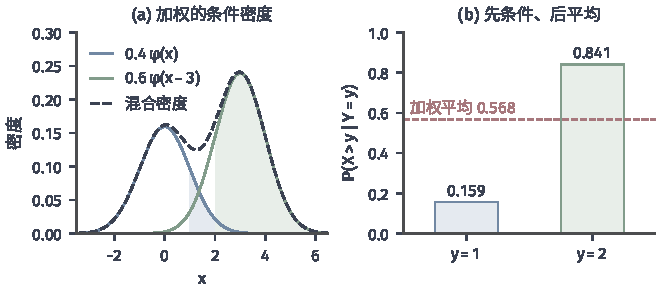
\includegraphics[width=112mm]{figures/02-abstract-mathematics/02-probability-spaces/matplotlib/cond-mixture-two-stage/figure.pdf}
  \caption{有限混合分布中“先条件、后平均”的计算。$\mathbb P(Y=1)=0.4$，$\mathbb P(Y=2)=0.6$，给定$Y=1,2$时$X$分别服从$N(0,1)$与$N(3,1)$，$\varphi$为标准正态密度。(a)加权条件密度与混合密度（虚线），阴影为$x>y$的区域；(b)两类别下的条件概率$\mathbb P(X>y\mid Y=y)$及其加权平均$0.568$（红色虚线）。}
  \label{fig:cond-mixture-two-stage}
\end{figure}

\subsection{条件密度与Bayes公式}

\paragraph{由联合密度构造条件核}
具体计算条件核时，最常见的情形是联合分布有密度。
设$\lambda_E,\lambda_D$分别是$E,D$上的$\sigma$有限测度，$(X,Y)$的联合分布关于$\lambda_E\otimes\lambda_D$有密度$p(x,y)$。
由Tonelli定理，$Y$的边缘密度$p_Y(y)=\int_Ep(x,y)\,\lambda_E(dx)$可测，且$P_Y(dy)=p_Y(y)\lambda_D(dy)$。

\begin{lemma}[条件密度给出条件核]
\label{lem:cond-density-kernel}
在上述设定下，固定$E$上一个概率测度$\nu$，令
\[
  K(y,dx)=
  \begin{cases}
    \dfrac{p(x,y)}{p_Y(y)}\,\lambda_E(dx), & 0<p_Y(y)<\infty,\\[1ex]
    \nu(dx), & \text{其他}.
  \end{cases}
\]
则$K$是$X$给定$Y$的条件核。
\end{lemma}

\begin{proof}
$K$对每个$y$是概率测度，可测性由Tonelli定理得到。只需验证式~\eqref{eq:cond-kernel-disintegration}。
记$G=\{0<p_Y<\infty\}$。由于$\int p_Y\,d\lambda_D=1$，$\lambda_D(\{p_Y=\infty\})=0$；又$P_Y(\{p_Y=0\})=\int_{\{p_Y=0\}}p_Y\,d\lambda_D=0$，所以$P_Y(G^c)=0$。对$B\in\mathcal E$，$C\in\mathcal D$，
\[
  \begin{aligned}
  \int_CK(y,B)\,P_Y(dy)&=\int_{C\cap G}\Bigl(\int_B\frac{p(x,y)}{p_Y(y)}\lambda_E(dx)\Bigr)p_Y(y)\,\lambda_D(dy)\\
  &=\int_{C\cap G}\int_Bp(x,y)\,\lambda_E(dx)\,\lambda_D(dy).
  \end{aligned}
\]
在$\{p_Y=0\}$上，$\int_Bp(x,y)\lambda_E(dx)\leq p_Y(y)=0$；$\{p_Y=\infty\}$是$\lambda_D$零集。所以把积分区域从$C\cap G$扩大到$C$不改变数值，结果为$\mathbb P(X\in B,Y\in C)$。
\end{proof}

比值$p(x,y)/p_Y(y)$就是\term{条件密度}（conditional density）。
它只给出条件核的一个合法版本：怎样补选$\nu$，乃至在一个$\lambda_E\otimes\lambda_D$零集上修改联合密度，都只让核在一个$P_Y$零集上改变，不影响结论。
反过来，没有联合密度时条件核仍然可以存在，例如确定性关系$X=f(Y)$对应的核$\delta_{f(y)}$。

\paragraph{Bayes公式}
统计模型往往按相反的方向给出：先给出未知类别或参数$X$的分布$\mu$，再给出给定$X=x$时观测$Y$的规律。
我们想由此求出给定观测$Y=y$后$X$的条件分布。

\begin{theorem}[Bayes公式]
\label{thm:cond-bayes}
设$X$取值于$(E,\mathcal E)$，分布为$\mu$；$\lambda$是$(D,\mathcal D)$上的$\sigma$有限测度，$\ell:D\times E\to[0,\infty)$对$\mathcal D\otimes\mathcal E$可测，且对每个$x$有$\int_D\ell(y\mid x)\,\lambda(dy)=1$。
设$Y$给定$X$的条件核为$\ell(y\mid x)\lambda(dy)$。令
\[
  q(y)=\int_E\ell(y\mid u)\,\mu(du).
\]
则$P_Y$关于$\lambda$的密度为$q$，集合$\{0<q<\infty\}$的$P_Y$概率为$1$；固定$E$上一个概率测度$\nu$，
\[
  K(y,dx)=
  \begin{cases}
    \dfrac{\ell(y\mid x)\,\mu(dx)}{q(y)}, & 0<q(y)<\infty,\\[1ex]
    \nu(dx), & \text{其他}
  \end{cases}
\]
是$X$给定$Y$的条件核。
\end{theorem}

\begin{proof}
由式~\eqref{eq:cond-kernel-disintegration}及其后的说明（交换$X,Y$的角色），$(X,Y)$的联合分布就是定理~\ref{thm:cond-kernel-joint}由$\mu$与核$\ell(y\mid x)\lambda(dy)$构造的$\mu(dx)\,\ell(y\mid x)\lambda(dy)$。对$B\in\mathcal E$，$C\in\mathcal D$，用一般Tonelli定理交换积分次序（$\mu$是概率测度，$\lambda$是$\sigma$有限测度），
\[
  \begin{aligned}
  \mathbb P(X\in B,Y\in C)&=\int_B\int_C\ell(y\mid x)\,\lambda(dy)\,\mu(dx)\\
  &=\int_C\Bigl(\int_B\ell(y\mid x)\,\mu(dx)\Bigr)\lambda(dy).
  \end{aligned}
\]
取$B=E$得$P_Y(C)=\int_Cq\,d\lambda$。与引理~\ref{lem:cond-density-kernel}的证明相同，$\int q\,d\lambda=1$推出$\{q=\infty\}$是$\lambda$零集，而$P_Y(\{q=0\})=0$。于是
\[
  \begin{aligned}
  \int_CK(y,B)\,P_Y(dy)&=\int_{C\cap\{0<q<\infty\}}\frac{\int_B\ell(y\mid x)\mu(dx)}{q(y)}\,q(y)\,\lambda(dy)\\
  &=\mathbb P(X\in B,Y\in C),
  \end{aligned}
\]
最后一步再次用到：在$\{q=0\}$上$\int_B\ell(y\mid x)\mu(dx)\leq q(y)=0$。
\end{proof}

公式中$\mu$称为先验分布，$\ell(y\mid\cdot)$作为$x$的函数是似然，$K(y,\cdot)$是后验分布；分母$q(y)$只起归一化作用。
定理只要求观测规律关于一个共同的参考测度$\lambda$有密度，对$X$的分布$\mu$没有任何密度要求：$\mu$可以是离散的、连续的或二者的混合。
公式在$P_Y$几乎处处的观测值上有效；在$q(y)=0$或$q(y)=\infty$的观测值上它不给出信息，而这些观测值合起来只构成$P_Y$零集。

\begin{example}[离散类别与连续观测]
\label{ex:cond-bayes-classes}
设类别$X\in\{0,1\}$，$\mathbb P(X=1)=0.3$；给定$X=0$时$Y\sim N(-1,1)$，给定$X=1$时$Y\sim N(1,1)$。
取$\lambda$为Lebesgue测度，$\ell(y\mid x)$为相应正态密度。由于$\ell(y\mid1)/\ell(y\mid0)=e^{2y}$，Bayes公式给出
\[
  \mathbb P(X=1\mid Y=y)=\frac{0.3\,\ell(y\mid1)}{0.3\,\ell(y\mid1)+0.7\,\ell(y\mid0)}=\frac{1}{1+\frac{7}{3}e^{-2y}}.
\]
$y=0$时后验概率等于先验$0.3$，因为两类似然相等；$y=1$时约为$0.760$。
这里$X$只取两个值，没有Lebesgue密度，但条件核照样存在。
\end{example}

图~\ref{fig:cond-bayes-posterior}左图是先验加权的两条似然曲线及其和$q(y)$；在每个观测值$y$处，绿色曲线占虚线高度的比例就是后验概率。
右图是后验概率随$y$变化的曲线：观测越靠右，越支持类别$1$；先验从$0.3$变为$0.5$时，整条曲线向左平移，$y=1$处的后验从$0.760$升到$0.881$。
统计模型中参数的估计、识别和推断程序不在本章范围，留到\BookPartRef{part:inference-and-causal-identification}{卷四“推断与因果识别”部分}。

\begin{figure}[htbp]
  \centering
  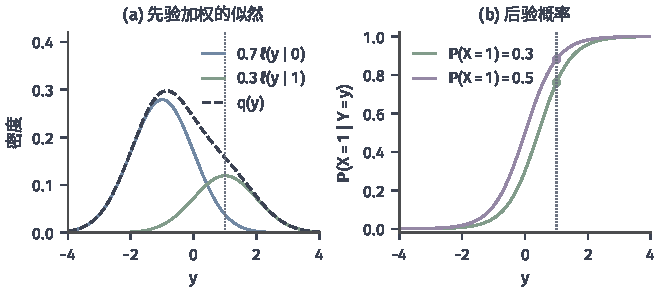
\includegraphics[width=112mm]{figures/02-abstract-mathematics/02-probability-spaces/matplotlib/cond-bayes-posterior/figure.pdf}
  \caption{离散类别与连续观测的Bayes后验。类别$X\in\{0,1\}$，给定$X=0,1$时$Y$分别服从$N(-1,1)$与$N(1,1)$，$\ell$为相应密度。(a)先验$\mathbb P(X=1)=0.3$时的加权似然及其和$q(y)$（虚线）；(b)先验为$0.3$与$0.5$时的后验概率$\mathbb P(X=1\mid Y=y)$，点线标出$y=1$，对应后验约为$0.760$与$0.881$。}
  \label{fig:cond-bayes-posterior}
\end{figure}

\section{条件独立}
\label{sec:cond-independence}

条件分布让我们能够提出一个更细的问题：在已知某些信息之后，另一项观测是否还会改变我们对$X$的判断？
本节用条件概率的乘积分解定义条件独立，给出它的函数判据与核判据，再说明它怎样简化信息依赖，以及它为什么不同于无条件的独立。

\subsection{条件独立的定义与判据}

\paragraph{条件独立的定义}
第~\ref{chap:probability-models}章用联合概率等于边缘概率之积定义独立（定义~\ref{def:pmod-independence}）。
把其中的概率换成给定信息下的条件概率，就得到条件独立。

\begin{definition}[条件独立]
\label{def:cond-independence}
设$X,Y$分别取值于$(E_1,\mathcal E_1)$与$(E_2,\mathcal E_2)$，$\mathcal G\subseteq\mathcal F$是子$\sigma$代数。
若对每个$A\in\mathcal E_1$、$B\in\mathcal E_2$，
\[
  \mathbb P(X\in A,\,Y\in B\mid\mathcal G)=\mathbb P(X\in A\mid\mathcal G)\,\mathbb P(Y\in B\mid\mathcal G)\qquad\text{几乎必然},
\]
则称$X$与$Y$给定$\mathcal G$\term{条件独立}（conditionally independent），记作$X\perp Y\mid\mathcal G$。$\mathcal G=\sigma(Z)$时记作$X\perp Y\mid Z$。
\end{definition}

等式对每一对$(A,B)$各自几乎必然成立，例外零集可以随$(A,B)$变化。
取$\mathcal G=\{\varnothing,\Omega\}$，条件概率就是普通概率，定义回到$X\perp Y$。

\paragraph{有界测试函数判据}
与独立性一样，事件上的乘积分解可以推广到函数。

\begin{lemma}[条件独立的函数判据]
\label{lem:cond-independence-functions}
$X\perp Y\mid\mathcal G$成立，当且仅当对所有有界可测函数$f:E_1\to\mathbb R$、$g:E_2\to\mathbb R$，
\[
  \mathbb E[f(X)g(Y)\mid\mathcal G]=\mathbb E[f(X)\mid\mathcal G]\,\mathbb E[g(Y)\mid\mathcal G]\qquad\text{几乎必然}.
\]
\end{lemma}

\begin{proof}
若函数形式的等式成立，取$f=\mathbb I_A$，$g=\mathbb I_B$即得条件独立。
反过来，若条件独立成立，两边关于$f$和$g$分别线性，所以等式对简单函数$f,g$成立。
对有界可测的$f,g$，取简单函数$f_n\to f$、$g_n\to g$逐点收敛且$|f_n|\leq\sup|f|$、$|g_n|\leq\sup|g|$；由条件控制收敛定理~\ref{thm:cond-dominated}，左边与右边两个因子都几乎必然收敛到相应的极限，于是等式对$f,g$成立。
\end{proof}

\paragraph{用条件核表述}
定义中每一对事件各带一个零集，读起来不如“在每个给定的条件下，联合分布是乘积”直观。
在标准Borel值域下，条件核让后一种说法变得准确。

设$X,Y$取值于标准Borel空间，$Z$取值于可测空间$(D,\mathcal D)$。$E_1\times E_2$仍是标准Borel空间，由定理~\ref{thm:cond-regular-existence}，$(X,Y)$给定$Z$的条件核$K_{XY}$存在。令$K_X(z,A)=K_{XY}(z,A\times E_2)$，$K_Y(z,B)=K_{XY}(z,E_1\times B)$，它们分别是$X$与$Y$给定$Z$的条件核。

\begin{theorem}[条件独立的核判据]
\label{thm:cond-independence-kernel}
在上述设定下，$X\perp Y\mid Z$成立，当且仅当存在$P_Z$零集$N$，使对每个$z\notin N$，
\[
  K_{XY}(z,\cdot)=K_X(z,\cdot)\otimes K_Y(z,\cdot).
\]
\end{theorem}

\begin{proof}
若核等式成立，在矩形$A\times B$上取值并代入$z=Z$，得$\mathbb P(X\in A,Y\in B\mid Z)=K_X(Z,A)K_Y(Z,B)=\mathbb P(X\in A\mid Z)\mathbb P(Y\in B\mid Z)$几乎必然成立。
反过来，取$E_1,E_2$各自的可数生成$\pi$系统$\mathcal C_1,\mathcal C_2$（分别包含$E_1,E_2$）。矩形族$\{A\times B:A\in\mathcal C_1,B\in\mathcal C_2\}$是可数$\pi$系统，并生成乘积$\sigma$代数。对其中每个矩形，条件独立给出$K_{XY}(z,A\times B)=K_X(z,A)K_Y(z,B)$在一个$P_Z$零集外成立；可数个零集的并$N$仍是零集。对$z\notin N$，两个概率测度$K_{XY}(z,\cdot)$与$K_X(z,\cdot)\otimes K_Y(z,\cdot)$在生成$\pi$系统上一致，由定理~\ref{thm:measure-uniqueness}，它们相等。
\end{proof}

定理说：固定一个有效的条件输入$z$之后，联合分布中不再有超出两个边缘分布的依赖。
证明中的关键仍然是可数生成族：只有可数个矩形的例外零集可以合并。
所以不要把每个事件对各自成立的版本等式，直接当作已经逐点一致的核等式；从前者到后者，需要先有条件核，再借助可数生成族。

\subsection{条件独立与信息简化}

\paragraph{已知$Z$后$Y$不再提供信息}
条件独立最常用的推论是删去多余的条件。
直观上，若给定$Z$后$X$与$Y$独立，那么已经知道$Z$时，再知道$Y$不会改变对$X$的平均判断。

\begin{theorem}[条件独立下的信息简化]
\label{thm:cond-independence-reduction}
设$X,Y,Z$是随机对象。若$X\perp Y\mid Z$，则对每个有界可测函数$f$，
\[
  \mathbb E[f(X)\mid Y,Z]=\mathbb E[f(X)\mid Z]\qquad\text{几乎必然}.
\]
反之，若上式对所有有界可测$f$成立，则$X\perp Y\mid Z$。
\end{theorem}

\begin{proof}
记$W=\mathbb E[f(X)\mid Z]$，它对$\sigma(Z)\subseteq\sigma(Y,Z)$可测。事件$\{Y\in B\}\cap\{Z\in C\}$构成包含$\Omega$并生成$\sigma(Y,Z)$的$\pi$系统，由引理~\ref{lem:cond-pi-check}，只需在这些事件上检验积分。利用全期望公式、函数判据（引理~\ref{lem:cond-independence-functions}）和提出已知因子，
\[
  \begin{aligned}
  \mathbb E[f(X)\mathbb I_B(Y)\mathbb I_C(Z)]
  &=\mathbb E\bigl[\mathbb I_C(Z)\,\mathbb E[f(X)\mathbb I_B(Y)\mid Z]\bigr]\\
  &=\mathbb E\bigl[\mathbb I_C(Z)\,W\,\mathbb E[\mathbb I_B(Y)\mid Z]\bigr]\\
  &=\mathbb E\bigl[\mathbb E[W\mathbb I_C(Z)\mathbb I_B(Y)\mid Z]\bigr]
  =\mathbb E[W\mathbb I_B(Y)\mathbb I_C(Z)],
  \end{aligned}
\]
其中第三个等号把有界的$\sigma(Z)$可测因子$W\mathbb I_C(Z)$放回条件期望之内。所以$W=\mathbb E[f(X)\mid Y,Z]$。

反过来，设上式对所有有界可测$f$成立。对有界可测$g$，由塔式法则（$\sigma(Z)\subseteq\sigma(Y,Z)$）与提出已知因子，
\[
  \begin{aligned}
  \mathbb E[f(X)g(Y)\mid Z]&=\mathbb E\bigl[g(Y)\,\mathbb E[f(X)\mid Y,Z]\bigm|Z\bigr]\\
  &=\mathbb E\bigl[g(Y)\,\mathbb E[f(X)\mid Z]\bigm|Z\bigr]=\mathbb E[f(X)\mid Z]\,\mathbb E[g(Y)\mid Z],
  \end{aligned}
\]
由引理~\ref{lem:cond-independence-functions}得$X\perp Y\mid Z$。
\end{proof}

反向判别需要对\emph{全部}有界可测$f$成立；只对某一个$f$成立，例如只知道条件均值不依赖$Y$，并不能推出条件独立。

\begin{example}[共享类别的两个比特]
\label{ex:cond-shared-class}
设类别$Z\in\{0,1\}$，$\mathbb P(Z=0)=\mathbb P(Z=1)=\frac12$。给定$Z=z$时，$X,Y$独立且都服从$\operatorname{Bernoulli}(p_z)$，取$p_0=0.2$，$p_1=0.8$。
按构造$X\perp Y\mid Z$，由定理~\ref{thm:cond-independence-reduction}，
\[
  \mathbb P(X=1\mid Y,Z)=\mathbb P(X=1\mid Z)=p_Z.
\]
知道类别后，$Y$的取值不再改变$X=1$的概率。
可是不给定$Z$时，$\mathbb P(X=1)=\mathbb P(Y=1)=0.5$，而
\[
  \mathbb P(X=1,Y=1)=\tfrac12(0.2^2+0.8^2)=0.34\neq0.25,
\]
所以$X$与$Y$并不独立：$\mathbb P(X=1\mid Y=1)=0.68$。$Y=1$让类别$1$更可信，从而间接提高了$X=1$的概率。
\end{example}

\paragraph{条件化可能产生依赖}
条件独立与独立互不蕴含。上例是条件独立而不独立；反方向的例子来自第~\ref{chap:probability-models}章的两个独立公平比特（示例~\ref{ex:pmod-xor-bits}）。
设$X,Y$独立且各以概率$\frac12$取$0,1$，$Z=X\oplus Y$为模二和。那里用这个例子区分两两独立与相互独立；这里用它检验条件化的影响。
给定$Z=0$，必有$Y=X$，于是
\[
  \begin{aligned}
  \mathbb P(X=1,Y=1\mid Z=0)&=\tfrac12,\\
  \mathbb P(X=1\mid Z=0)\,\mathbb P(Y=1\mid Z=0)&=\tfrac12\times\tfrac12=\tfrac14.
  \end{aligned}
\]
这里$\mathbb P(X=1\mid Z=0)=\frac12$，因为$X$与$Z$独立。给定$Z$后知道$X$就确定了$Y$，原本的独立性消失了。

图~\ref{fig:cond-independence-tables}并排列出两个例子的联合概率表。
上排中，给定$Z=0$或$Z=1$时的表都是外积，但按$Z$平均后对角格变大，不再是边缘的乘积；下排中，无条件的表是均匀的乘积，给定$Z$后质量集中到对角或反对角，不再是乘积。

\begin{figure*}[htbp]
  \centering
  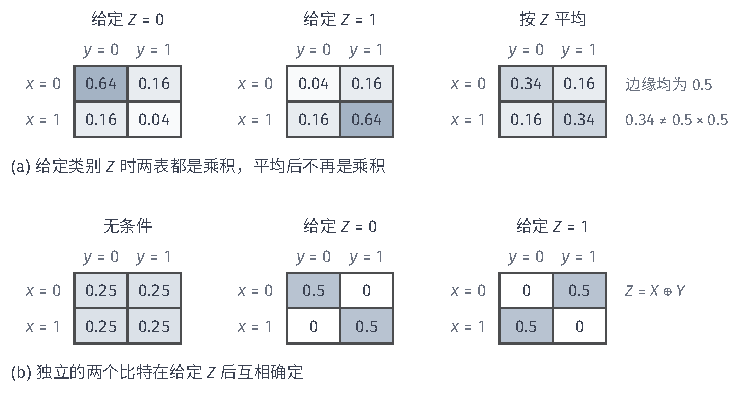
\includegraphics[width=125mm]{figures/02-abstract-mathematics/02-probability-spaces/tikz/cond-independence-tables/figure.pdf}
  \caption{条件独立与条件化后出现的依赖，表中为$(X,Y)$的联合概率，底色深浅与概率成正比。(a)$\mathbb P(Z=0)=\mathbb P(Z=1)=\frac12$，给定$Z=z$时$X,Y$独立同分布于$\operatorname{Bernoulli}(p_z)$，$p_0=0.2$，$p_1=0.8$：两张条件表都是乘积，平均后$\mathbb P(X=1,Y=1)=0.34$，大于边缘乘积$0.25$。(b)$X,Y$为独立公平比特，$Z=X\oplus Y$：无条件表为乘积，给定$Z=0$或$Z=1$后只剩两格。}
  \label{fig:cond-independence-tables}
\end{figure*}

条件独立始终是给定联合分布之内的关系，它说明的是“已知$Z$时$Y$对$X$不再提供信息”。
它本身不说明改变$Y$是否会影响$X$：干预、因果效应及其识别需要额外的模型与假设，归卷四推断与因果识别部分讨论。

\section{本章小结}
\label{sec:cond-summary}

章首问的是：观测取连续值、每个观测值的概率都是零时，给定观测的平均和分布指什么。
本章的回答从有限分组中的条件平均开始。
分组平均有两项性质：只依赖可用的信息，在每个可观察事件上保持积分总量。
条件期望把这两项性质原样作为定义，完全不做除法，因此对零概率的观测值同样有意义；Radon--Nikodym定理保证它对任意子$\sigma$代数存在，并且几乎必然唯一。
给定观测$Y$时，Doob--Dynkin引理把它写成观测值的函数$h(Y)$，$h$在$P_Y$几乎处处的意义下确定。

从同一个定义出发，我们得到可以直接使用的几组规则。
线性、保序、提出已知因子和塔式法则支撑日常计算，其中提出因子需要$X$与$HX$可积，塔式法则需要两个信息有包含关系。
条件Jensen不等式给出矩与平均误差的收缩；条件均方误差分解说明，在只依据给定信息的平方可积预测中，条件平均的均方误差最小。
条件单调收敛、条件Fatou与条件控制收敛在固定信息下交换条件期望与极限，控制变量可积是避免$\infty-\infty$的条件。

第二个问题是怎样用一个对象同时给出所有事件的条件概率。
概率核提供了这样的对象：它由输入分布构造联合分布，复合时对中间状态求平均。
条件分布就是满足逐事件条件的概率核；逐事件的条件概率总是存在，但把它们拼成分布需要检查取值空间的可测结构，本书使用的充分条件是取值于标准Borel空间。
条件核在一个共同的$P_Y$零集外唯一，用它可以统一计算各种条件平均，有密度时由条件密度或Bayes公式写出。
条件独立则用条件核表达“已知$Z$后$Y$不再提供信息”，它与独立互不蕴含，也不等同于因果关系。

零概率观测值上的版本自由贯穿全章：条件期望、条件核和条件密度都只在几乎处处意义下确定。
第~\ref{chap:random-variable-convergence}章将用本章的收缩估计和条件极限定理研究随机变量列的平均收敛；条件期望的投影结构留给第~\ref{part:function-spaces}部分，随时间增加的信息与过程模型留给卷三。

\chapter{随机变量的收敛与积分极限}
\label{chap:random-variable-convergence}

设想我们用计算机反复抛一枚均匀硬币，每抛一次就更新一次正面出现的频率。
卷一的弱大数律告诉我们：频率偏离$1/2$超过$0.01$的概率随抛掷次数$n$增大而趋于零。
可是我们真正手里拿着的，是\emph{这一次}运行产生的一整条频率序列。
这条序列本身会不会收敛到$1/2$？还是说它每隔一段时间仍可能跳出去一次，只是跳出去的时刻越来越难以预料？
概率很小的坏事件，与坏事件最终不再发生，是两种不同的保证。

另一类问题出在期望上。
设一列随机误差在几乎每个样本结果上都趋于零，它们的平均误差是否也趋于零？
直觉上似乎理所当然，但只要误差偶尔取非常大的值，答案就可能是否定的。
在估计、模拟和学习算法的分析中，我们经常先得到随机量的某种极限，再想把极限传到期望、风险或条件期望里去；何时允许这样做，需要明确的条件。

本章固定一个概率空间，研究其上随机变量列的极限，回答三个相连的问题：随机误差以什么意义趋于零；随机变量的极限何时能传入期望；独立样本的平均何时沿几乎每条样本序列趋于总体均值。
第~\ref{sec:conv-modes}节从样本点上的数值、误差超过阈值的概率和平均误差三个角度定义收敛，比较它们的强弱并给出反例。
这些反例的差别归结为“坏事件是否发生无穷多次”这一集合问题，第~\ref{sec:conv-events}节为此建立事件列的上、下极限与Borel--Cantelli引理，并由此得到依概率收敛的子列判据。
第~\ref{sec:conv-expectation-limits}节用子列判据把积分收敛定理推广到依概率收敛，再用一致可积刻画平均误差何时随随机变量一起趋于零。
最后两节转向独立和：第~\ref{sec:conv-partial-sums}节控制部分和在整个过程中的最大偏差，得到随机级数的收敛判据和Kronecker引理；第~\ref{sec:conv-sample-means}节把这些工具与截断结合，证明有限一阶矩下的强大数律。

\section{收敛方式及其基本关系}
\label{sec:conv-modes}

本节固定概率空间$(\Omega,\mathcal F,\mathbb P)$及其上的实值随机变量$X_1,X_2,\ldots$与$X$。
随机变量是样本结果的函数，所以“$X_n$趋于$X$”至少有三种自然的读法：对每个样本结果看数列，对每个$n$看误差超过阈值的概率，或者对每个$n$看误差的平均大小。
我们依次定义这三种收敛，再比较它们之间的蕴含关系，并用两个可以直接计算的例子说明哪些逆命题不成立。

\subsection{几乎处处收敛}

\paragraph{逐个样本结果上的数列}
固定一个样本结果$\omega$，$X_1(\omega),X_2(\omega),\ldots$就是一列普通实数，可以问它是否收敛到$X(\omega)$。
要求所有$\omega$都收敛往往太苛刻：随机变量只在相差零概率事件的意义下确定，改动一个零概率事件上的取值不应改变我们对极限的判断。
因此只要求收敛在一个概率为$1$的事件上成立。

\begin{definition}[几乎处处收敛]
\label{def:conv-almost-sure}
若存在事件$A\in\mathcal F$，$\mathbb P(A)=1$，使每个$\omega\in A$都满足$X_n(\omega)\to X(\omega)$，则称$X_n$\term{几乎处处收敛}（almost sure convergence）于$X$，记作$X_n\xrightarrow{\mathrm{a.s.}}X$。
\end{definition}

在概率空间中，“几乎处处”与第~\ref{chap:probability-models}章定义~\ref{def:pmod-almost-sure}所说的“几乎必然”是同一个意思，都指在一个概率为$1$的事件上成立；所以几乎处处收敛也叫几乎必然收敛，记号中的$\mathrm{a.s.}$正取自almost surely。

定义里要求“存在”一个概率为$1$的事件，但所有使数列收敛的$\omega$组成的集合本身是不是事件？
数列收敛意味着对每个误差阈值，从某一项起误差都不超过它；阈值只需取$1/m$，$m=1,2,\ldots$，于是
\begin{equation}
  \{\omega:X_n(\omega)\to X(\omega)\}
  =\bigcap_{m=1}^{\infty}\bigcup_{N=1}^{\infty}\bigcap_{n=N}^{\infty}\Bigl\{|X_n-X|\leq\frac1m\Bigr\}.
  \label{eq:conv-convergence-event}
\end{equation}
右侧每个$\{|X_n-X|\leq1/m\}$都是事件，而所有交与并都是可数次的，所以收敛集合是事件。
几乎处处收敛就是说这个事件的概率为$1$。

\paragraph{起始位置依赖样本结果}
式~\eqref{eq:conv-convergence-event}中“从第$N$项起”的$N$由关于$N$的并引入，只要求存在，因此它可以随$\omega$和阈值$1/m$变化。
取$\Omega=[0,1)$，$\mathbb P$为长度，令$X_n(\omega)=\omega^n$。
每个$\omega\in[0,1)$都有$\omega^n\to0$，所以$X_n\xrightarrow{\mathrm{a.s.}}0$，而且这里的收敛对每个样本点都成立。
但要使误差不超过$0.01$，$\omega=0.9$需要$n\geq44$，$\omega=0.99$则需要$n\geq459$；$\omega$越接近$1$，所需的项数越大，不存在一个对所有$\omega$都够用的$N$。
几乎处处收敛并不要求误差在同一时刻对所有样本结果同时变小，它只要求每个样本结果最终都会进入并停留在任意小的误差范围内。

\paragraph{零概率例外的合并}
随机变量通常只在几乎必然相等的意义下确定。
若对每个$n$，$X_n'$与$X_n$只在零概率事件$N_n$上不同，$X'$与$X$只在零概率事件$N_0$上不同，那么在$N=N_0\cup\bigcup_nN_n$之外两列取值完全相同。
可数个零概率事件的并仍是零概率事件，所以$X_n\xrightarrow{\mathrm{a.s.}}X$当且仅当$X_n'\xrightarrow{\mathrm{a.s.}}X'$：逐项更换版本不影响几乎处处收敛。

这一步依赖于例外集合只有可数个。
仍取$\Omega=[0,1)$与长度测度，若把下标换成连续时刻$t\in[0,1)$，令$Y_t(\omega)=\mathbb I_{\{\omega=t\}}$，则每个$Y_t$都几乎必然等于$0$，但对每个$\omega$都有$\sup_tY_t(\omega)=1$；不可数个零概率例外合并后可以占满整个样本空间。
本章只讨论可数的随机变量列，连续时间的版本选择问题留给随机过程的讨论。

\subsection{依概率收敛}

\paragraph{坏事件的概率}
几乎处处收敛关心每个样本结果的整条数列。
另一种更容易计算的要求只看每个固定的$n$：误差超过阈值的事件，其概率是否趋于零。
卷一讨论样本均值时已经用过这一要求，这里把它放到一般概率空间上。

\begin{definition}[依概率收敛]
\label{def:conv-probability}
若对每个$\varepsilon>0$都有
\[
  \lim_{n\to\infty}\mathbb P\bigl(|X_n-X|>\varepsilon\bigr)=0,
\]
则称$X_n$\term{依概率收敛}（convergence in probability）于$X$，记作$X_n\xrightarrow{\mathbb P}X$。
\end{definition}

卷一的定义用的是$\geq\varepsilon$，这里用$>\varepsilon$，两者等价：$\{|X_n-X|\geq\varepsilon\}$夹在$\{|X_n-X|>\varepsilon/2\}$与$\{|X_n-X|>\varepsilon\}$之间，而$\varepsilon$是任意的。
从测度论的角度看，依概率收敛就是概率测度下的\term{依测度收敛}（convergence in measure）。
称$A_n(\varepsilon)=\{|X_n-X|>\varepsilon\}$为第$n$项的\emph{坏事件}；依概率收敛控制的是每个坏事件的大小，却没有要求同一个样本结果在某一项以后不再落入坏事件。
关于有限方差和有限一阶矩下样本均值依概率收敛的证明，可参考\BookChapterRef{chap:sampling-errors}{卷一“抽样分布与估计误差”章}；本章第~\ref{sec:conv-sample-means}节会在那里结论的基础上讨论几乎处处收敛。

\paragraph{二进区间扫描}
下面的例子让坏事件越来越小，却让每个样本结果反复落入坏事件。
后面讨论平均收敛、蕴含关系的反例和子列判据时，还会回到这个例子。

\begin{example}[二进区间扫描]
\label{ex:conv-dyadic-sweep}
取$U\sim\mathrm{Unif}[0,1)$。每个正整数唯一地写成$n=2^k+j$，其中$k\geq0$，$0\leq j<2^k$，令
\[
  X_n=\mathbb I_{\{U\in[j/2^k,(j+1)/2^k)\}}.
\]
$n=1$对应整个区间$[0,1)$；$n=2,3$把它分成两半；$n=4,\ldots,7$把它分成四段；以此类推，第$k$轮依次扫过长度为$2^{-k}$的$2^k$个区间。
于是对$0<\varepsilon<1$，第$k$轮中的每一项都满足$\mathbb P(|X_n|>\varepsilon)=\mathbb P(X_n=1)=2^{-k}$。
当$n\to\infty$时$k=\lfloor\log_2n\rfloor\to\infty$，所以$X_n\xrightarrow{\mathbb P}0$。

另一方面，固定$U$的一个取值$u\in[0,1)$。每一轮的$2^k$个区间恰好覆盖$[0,1)$且互不相交，所以每一轮恰有一项取$1$，其余项取$0$。
数列$X_n(u)$中因此有无穷多个$1$和无穷多个$0$，不收敛。
例如$u=0.3$时，第$k$轮中取$1$的是$j=\lfloor0.3\cdot2^k\rfloor$那一项，即$n=1,2,5,10,20,41,83,\ldots$，每一轮一次。
\end{example}

图~\ref{fig:conv-dyadic-sweep}把这个例子画了出来。
左图中每条横线是使$X_n=1$的区间，竖虚线所在的$u=0.3$每一轮都恰好穿过一条红色横线。
右图把这条样本路径和“取$1$的概率”画在一起：概率每一轮减半，而路径上的$1$始终不会消失，只是两个$1$之间的间隔越来越长。
坏事件变小与坏事件停止发生，在这里明确地分开了。

\begin{figure*}[htbp]
  \centering
  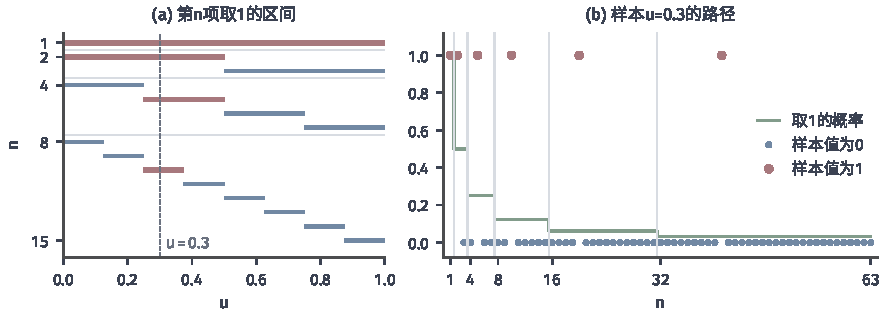
\includegraphics[width=150mm]{figures/02-abstract-mathematics/02-probability-spaces/matplotlib/conv-dyadic-sweep/figure.pdf}
  \caption{二进区间扫描$X_n=\mathbb I_{\{U\in[j/2^k,(j+1)/2^k)\}}$，$n=2^k+j$。(a) 前$15$项各自取$1$的区间，浅色横线分隔不同轮次，红色标出包含$u=0.3$的区间；(b) 样本$u=0.3$的路径$X_n(0.3)$，$n\leq63$（红点为$1$，蓝点为$0$），绿色阶梯为$\mathbb P(X_n=1)=2^{-k}$，竖线标出每一轮的起点$n=2^k$。}
  \label{fig:conv-dyadic-sweep}
\end{figure*}

\subsection{$p$阶平均收敛}

\paragraph{误差幅度的平均}
依概率收敛只问误差是否超过阈值，不问超过多少。
如果大误差虽然少见，一旦出现却非常大，我们往往希望把幅度也计入考虑，这就要对误差取平均。

\begin{definition}[$p$阶平均收敛]
\label{def:conv-mean}
设$1\leq p<\infty$，$\mathbb E|X_n|^p<\infty$对每个$n$成立，且$\mathbb E|X|^p<\infty$。若
\[
  \lim_{n\to\infty}\mathbb E|X_n-X|^p=0,
\]
则称$X_n$\term{$p$阶平均收敛}（convergence in $p$-th mean）于$X$，记作$X_n\xrightarrow{L^p}X$。
\end{definition}

记号$\xrightarrow{L^p}$只是“$\mathbb E|X_n-X|^p\to0$”的简写，本章不使用$L^p$作为函数空间的范数、完备性等结构，那些内容属于第~\ref{part:function-spaces}部分。
两个有限$p$阶矩的随机变量之差仍有有限$p$阶矩，因为$|a-b|^p\leq2^{p-1}(|a|^p+|b|^p)$（函数$t\mapsto t^p$在$[0,\infty)$上凸）。
$p=1$时$\mathbb E|X_n-X|$是平均绝对误差；$p=2$时$\mathbb E(X_n-X)^2$是均方误差，相应的收敛也叫\term{均方收敛}（mean-square convergence）。
$p$越大，大误差在平均中所占的分量越重：误差为$10$的事件在$p=1$时贡献$10$倍概率，在$p=2$时贡献$100$倍概率。

回到二进区间扫描。$X_n$只取$0$和$1$，所以对任意$p\geq1$，$\mathbb E|X_n|^p=\mathbb P(X_n=1)=2^{-k}\to0$，即$X_n\xrightarrow{L^p}0$。
这个例子在每一种平均意义下都收敛，却没有一个样本结果收敛。

\paragraph{有限维随机向量}
对取值于$\mathbb R^d$的随机向量$\bm X_n=(X_{n,1},\ldots,X_{n,d})$与$\bm X$，用欧氏范数代替绝对值：$\bm X_n\xrightarrow{L^p}\bm X$指$\mathbb E\lVert\bm X_n-\bm X\rVert_2^p\to0$。
它与逐坐标的$p$阶平均收敛等价。
记$\bm x\in\mathbb R^d$的坐标为$x_i$。一方面$|x_i|\leq\lVert\bm x\rVert_2$；另一方面
\[
  \lVert\bm x\rVert_2^p\leq\bigl(d\max_i|x_i|^2\bigr)^{p/2}=d^{p/2}\max_i|x_i|^p\leq d^{p/2}\sum_{i=1}^d|x_i|^p.
\]
把$\bm x=\bm X_n-\bm X$代入并取期望，得到
\[
  \mathbb E|X_{n,i}-X_i|^p\leq\mathbb E\lVert\bm X_n-\bm X\rVert_2^p\leq d^{p/2}\sum_{i=1}^d\mathbb E|X_{n,i}-X_i|^p,
\]
左式说明向量收敛蕴含每个坐标收敛，右式说明$d$个坐标都收敛时向量也收敛。
同样的两个不等式也说明，向量的几乎处处收敛和依概率收敛都与逐坐标的相应收敛等价；对依概率收敛，只需注意$\{\lVert\bm X_n-\bm X\rVert_2>\varepsilon\}\subseteq\bigcup_i\{|X_{n,i}-X_i|>\varepsilon/\sqrt d\}$。
这里只用到有限维的范数比较，维数$d$固定是关键：常数$d^{p/2}$随维数增大，无限维时不能照搬。
下文因此只对实值随机变量叙述结论。

\subsection{蕴含关系与反例}

\paragraph{三条蕴含与极限的唯一性}
有了三种定义，自然要问它们之间谁强谁弱。
下面的定理汇总能直接证明的蕴含关系。

\begin{theorem}[收敛方式之间的蕴含]
\label{thm:conv-implications}
设$X_n,X$是$(\Omega,\mathcal F,\mathbb P)$上的随机变量。
\begin{enumerate}
  \item 若$X_n\xrightarrow{\mathrm{a.s.}}X$，则$X_n\xrightarrow{\mathbb P}X$。
  \item 若对某个$1\leq p<\infty$有$X_n\xrightarrow{L^p}X$，则$X_n\xrightarrow{\mathbb P}X$。
  \item 若$1\leq p<q<\infty$且$X_n\xrightarrow{L^q}X$，则$X_n\xrightarrow{L^p}X$。
  \item 若$X_n\xrightarrow{\mathbb P}X$且$X_n\xrightarrow{\mathbb P}X'$，则$X=X'$几乎必然成立。
\end{enumerate}
\end{theorem}

\begin{proof}
(1) 固定$\varepsilon>0$。在使$X_n(\omega)\to X(\omega)$的概率为$1$的事件上，$\mathbb I_{\{|X_n-X|>\varepsilon\}}(\omega)$从某一项起恒为$0$，所以这些示性函数几乎处处趋于$0$；它们都以常数$1$为界，而常数$1$在概率测度下可积。
由控制收敛定理（定理~\ref{thm:integral-dominated-convergence}；常数控制的特例常称有界收敛定理），$\mathbb P(|X_n-X|>\varepsilon)=\mathbb E\,\mathbb I_{\{|X_n-X|>\varepsilon\}}\to0$。

(2) 第~\ref{chap:probability-models}章定理~\ref{thm:pmod-markov}的Markov不等式说，非负随机变量$Y$满足$\mathbb P(Y\geq t)\leq\mathbb EY/t$，$t>0$。取$Y=|X_n-X|^p$，$t=\varepsilon^p$，得
\[
  \mathbb P(|X_n-X|>\varepsilon)\leq\mathbb P(|X_n-X|^p\geq\varepsilon^p)\leq\frac{\mathbb E|X_n-X|^p}{\varepsilon^p}\to0.
\]

(3) 由第~\ref{chap:probability-models}章定理~\ref{thm:pmod-moment-monotone}，有限$q$阶矩蕴含有限$p$阶矩，所以$\mathbb E|X_n-X|^p$有定义。
令$Y=|X_n-X|^p\geq0$，函数$\varphi(t)=t^{q/p}$在$[0,\infty)$上凸，由定理~\ref{thm:pmod-jensen}的Jensen不等式$\varphi(\mathbb EY)\leq\mathbb E\varphi(Y)$，
\[
  \bigl(\mathbb E|X_n-X|^p\bigr)^{q/p}\leq\mathbb E|X_n-X|^q\to0.
\]

(4) 由三角不等式，$|X-X'|>2\varepsilon$时$|X_n-X|>\varepsilon$与$|X_n-X'|>\varepsilon$至少有一个成立，所以对每个$n$，
\[
  \mathbb P(|X-X'|>2\varepsilon)\leq\mathbb P(|X_n-X|>\varepsilon)+\mathbb P(|X_n-X'|>\varepsilon).
\]
左侧与$n$无关，右侧趋于$0$，故$\mathbb P(|X-X'|>2\varepsilon)=0$。
取$\varepsilon=1/m$，$\{X\neq X'\}=\bigcup_m\{|X-X'|>2/m\}$是可数个零概率事件的并，概率为$0$。
\end{proof}

结论(3)用到了$\mathbb P$是概率测度：Jensen不等式是对总质量为$1$的测度取平均才成立的，在Lebesgue测度这样的无穷测度上，$q$阶积分小并不能推出$p$阶积分小。
结论(3)的方向也不能颠倒，下文用尖峰的变形说明低阶平均收敛推不出高阶平均收敛。
结论(4)说明依概率极限在几乎必然相等的意义下唯一；由(1)和(2)，几乎处处极限与$p$阶平均极限也同样唯一，三种收敛若同时成立，极限必定一致。

\paragraph{两类反例}
上述蕴含能否反过来？
二进区间扫描已经回答了一半：它依概率收敛，也在每个$p$阶平均意义下收敛，却不几乎处处收敛。
所以依概率收敛和平均收敛都不能推出几乎处处收敛。
另一半需要一个方向相反的例子：误差几乎处处趋于零，平均误差却不趋于零。

\begin{example}[尖峰]
\label{ex:conv-spike}
取$U\sim\mathrm{Unif}[0,1)$，令$X_n=n\,\mathbb I_{\{0<U<1/n\}}$。
对每个$u\in(0,1)$，只要$n>1/u$就有$X_n(u)=0$；$u=0$时所有$X_n(0)=0$。所以每个样本结果上都有$X_n\to0$，$X_n\xrightarrow{\mathrm{a.s.}}0$。
但
\[
  \mathbb E|X_n|=n\cdot\mathbb P(0<U<1/n)=n\cdot\frac1n=1,
\]
平均误差恒为$1$，不趋于$0$；$p>1$时的平均误差$\mathbb E|X_n|^p=n^{p-1}$甚至趋于无穷。
\end{example}

图~\ref{fig:conv-spike}显示了尖峰的机制：$X_n$在越来越窄的区间$(0,1/n)$上取越来越大的值$n$，每个函数图像下的面积都是$1$。
样本$u=0.3$只在$n=1,2,3$处取到非零值，此后永远为$0$；取非零值的概率是$1/n$，也趋于零。
期望由面积决定，而面积从未减少，它只是被挤进了一个越来越小的事件里。

\begin{figure*}[htbp]
  \centering
  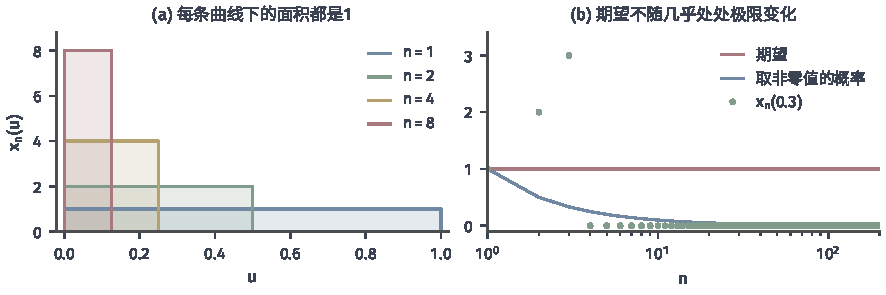
\includegraphics[width=150mm]{figures/02-abstract-mathematics/02-probability-spaces/matplotlib/conv-spike/figure.pdf}
  \caption{尖峰$X_n=n\,\mathbb I_{\{0<U<1/n\}}$，$U\sim\mathrm{Unif}[0,1)$。(a) 函数$x_n(u)=n\,\mathbb I_{(0,1/n)}(u)$在$n=1,2,4,8$时的图像，阴影面积均为$1$；(b) 横轴为对数刻度：$\mathbb E|X_n|$恒为$1$（红线），$\mathbb P(X_n\neq0)=1/n$（蓝线），绿点为样本$u=0.3$处的取值，$n\geq4$时均为$0$。}
  \label{fig:conv-spike}
\end{figure*}

两类例子分别暴露了两种不同的“坏”。
二进区间扫描中，误差每次出现时幅度都是$1$，但它反复出现，没有一条样本路径能摆脱它；尖峰中误差对每条路径只出现有限次，但出现时幅度极大，足以把平均误差维持在固定水平。
尖峰还满足$\mathbb P(|X_n|>\varepsilon)\leq1/n\to0$，所以它同时说明依概率收敛推不出一阶平均收敛。
类似地，取$1\leq p<q$，令$X_n=n^{1/q}\,\mathbb I_{\{0<U<1/n\}}$，则$\mathbb E|X_n|^p=n^{p/q-1}\to0$，而$\mathbb E|X_n|^q=1$，所以$p$阶平均收敛推不出$q$阶平均收敛。

图~\ref{fig:conv-implications}汇总了本节已证明的蕴含和三个反例。
图中没有单独画出的反向关系，可以由箭头与上面的例子组合判断。
例如，若依概率收敛蕴含$p$阶平均收敛，接在“几乎处处收敛蕴含依概率收敛”之后，就会得到几乎处处收敛蕴含$p$阶平均收敛，与尖峰矛盾；$p$阶平均收敛不能推出几乎处处收敛，则直接由二进区间扫描看出，因为它在每个$p$阶平均意义下都收敛，却没有一个样本结果收敛。
下两节的任务，是找出在什么附加条件下图中的虚线可以改成实线：第~\ref{sec:conv-events}节处理从依概率到几乎处处的方向，第~\ref{sec:conv-expectation-limits}节处理从几乎处处或依概率到平均收敛的方向。

\begin{figure*}[htbp]
  \centering
  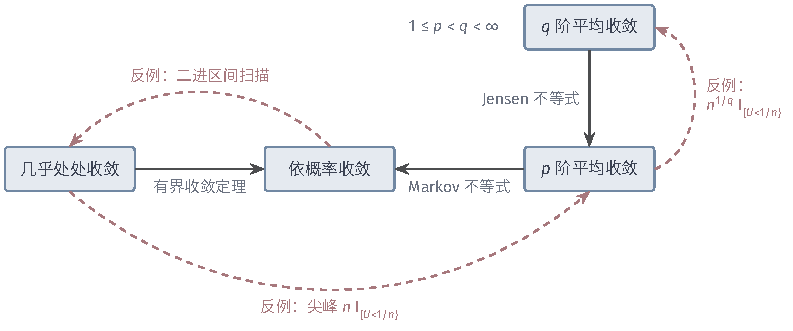
\includegraphics[width=134mm]{figures/02-abstract-mathematics/02-probability-spaces/tikz/conv-implications/figure.pdf}
  \caption{三种收敛方式的关系，$1\leq p<q<\infty$。黑色实线是定理~\ref{thm:conv-implications}证明的蕴含，旁注所用工具；红色虚线表示该方向的蕴含不成立，旁注反例，$U\sim\mathrm{Unif}[0,1)$。}
  \label{fig:conv-implications}
\end{figure*}

\section{事件列与收敛判据}
\label{sec:conv-events}

上一节的两类反例可以翻译成一个关于集合的问题：误差超过阈值的事件，是否发生无穷多次。
二进区间扫描中，每个样本结果都无穷多次落入坏事件；尖峰中，每个样本结果只落入有限次。
本节先给“无穷多次发生”和“最终总是发生”以精确的集合表示，再用概率的求和判断它们的概率，由此得到依概率收敛与几乎处处收敛之间的桥梁——子列判据；最后补充独立序列的尾事件只能取概率$0$或$1$的性质。

\subsection{事件的上极限与下极限}

\paragraph{无穷多次与最终总是}
设$A_1,A_2,\ldots$是一列事件。
说样本结果$\omega$属于“无穷多个$A_n$”，就是说无论走到多晚的位置$m$，后面总还有某个$n\geq m$使$\omega\in A_n$；
说$\omega$“最终总在$A_n$中”，就是说存在某个位置$m$，此后每个$n\geq m$都有$\omega\in A_n$。
把“对所有$m$”写成交、“存在$m$”写成并，得到如下定义。

\begin{definition}[事件列的上极限与下极限]
\label{def:conv-limsup-events}
事件列$(A_n)$的\term{上极限}（limit superior）与\term{下极限}（limit inferior）分别为
\[
  \limsup_{n\to\infty}A_n=\bigcap_{m=1}^{\infty}\bigcup_{n\geq m}A_n,\qquad
  \liminf_{n\to\infty}A_n=\bigcup_{m=1}^{\infty}\bigcap_{n\geq m}A_n.
\]
\end{definition}

两者的区别只在量词的顺序。
上极限先对每个$m$取“后面某一项”，再要求对所有$m$成立，所以$\omega\in\limsup_nA_n$当且仅当$\omega$属于无穷多个$A_n$，常写作$\{A_n\ \text{i.o.}\}$（infinitely often）。
下极限先固定某个$m$，再要求“后面每一项”，所以$\omega\in\liminf_nA_n$当且仅当$\omega$从某一项起属于所有$A_n$。
最终总在的样本结果当然也无穷多次出现，故$\liminf_nA_n\subseteq\limsup_nA_n$。
取补集时并与交互换，得到$(\limsup_nA_n)^c=\liminf_nA_n^c$：不属于无穷多个$A_n$，等价于最终总不属于$A_n$。
两者都由可数次交、并得到，所以都是事件。

图~\ref{fig:conv-limsup-liminf}用三个样本结果说明这两个集合。
$\omega_1$在所有偶数项中出现，次数无穷但始终有缺口，它属于上极限而不属于下极限；$\omega_2$在第$7$项之后不再出现，两者都不属于；$\omega_3$从第$8$项起每项都出现，属于下极限，也就属于上极限。
图中只能画出有限多列，判断依据是右侧所写的延续规律，而不是前$16$列。

\begin{figure*}[htbp]
  \centering
  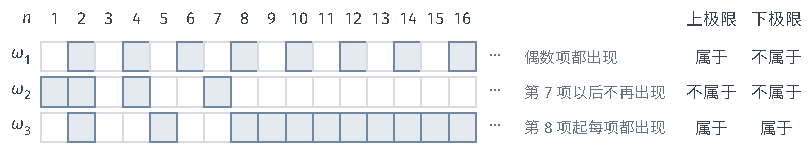
\includegraphics[width=138mm]{figures/02-abstract-mathematics/02-probability-spaces/tikz/conv-limsup-liminf/figure.pdf}
  \caption{事件列的上极限与下极限示意。第$\omega$行第$n$列的阴影格表示$\omega\in A_n$；三个样本结果的归属按右侧所写规律无限延续，最右两列给出它们是否属于$\limsup_nA_n$与$\liminf_nA_n$。}
  \label{fig:conv-limsup-liminf}
\end{figure*}

\paragraph{收敛与坏事件只发生有限次}
把坏事件代入上极限，就得到几乎处处收敛的事件刻画。
对$\varepsilon>0$，记$A_n(\varepsilon)=\{|X_n-X|>\varepsilon\}$。
数列$X_n(\omega)$收敛到$X(\omega)$，当且仅当对每个$\varepsilon>0$，$\omega$只属于有限多个$A_n(\varepsilon)$。
由于$A_n(\varepsilon)$随$\varepsilon$减小而增大，只需检查$\varepsilon=1/m$，于是
\[
  \{X_n\not\to X\}=\bigcup_{m=1}^{\infty}\limsup_{n\to\infty}A_n(1/m).
\]
这是式~\eqref{eq:conv-convergence-event}取补集后的形式。右侧是可数并，所以下面的判据成立。

\begin{lemma}[几乎处处收敛的事件判据]
\label{lem:conv-as-criterion}
$X_n\xrightarrow{\mathrm{a.s.}}X$，当且仅当对每个$\varepsilon>0$都有$\mathbb P\bigl(\limsup_nA_n(\varepsilon)\bigr)=0$。
\end{lemma}

\begin{proof}
若$X_n\xrightarrow{\mathrm{a.s.}}X$，每个$\limsup_nA_n(\varepsilon)$都包含于零概率事件$\{X_n\not\to X\}$。
反之，若每个$\limsup_nA_n(1/m)$概率为零，它们的可数并$\{X_n\not\to X\}$概率也为零。
\end{proof}

与依概率收敛比较，后者要求的是$\mathbb P(A_n(\varepsilon))\to0$。
由概率的连续性，$\bigcup_{n\geq m}A_n$随$m$递减到$\limsup_nA_n$，而每个$\bigcup_{n\geq m}A_n$的概率不小于其中任一$A_n$的概率，所以
\[
  \mathbb P\Bigl(\limsup_{n\to\infty}A_n\Bigr)=\lim_{m\to\infty}\mathbb P\Bigl(\bigcup_{n\geq m}A_n\Bigr)\geq\limsup_{n\to\infty}\mathbb P(A_n).
\]
这个不等式只给出上极限概率的下界。当单项概率$\mathbb P(A_n)$趋于$0$时，下界是$0$，它对上极限的概率没有提供任何信息。
二进区间扫描正是如此：$\mathbb P(A_n(1/2))=2^{-k}\to0$，但每个样本结果都无穷多次落入$A_n(1/2)$，$\limsup_nA_n(1/2)=\Omega$。
要从单项概率推出上极限的概率，需要更多信息，下一小节给出两种情形。

\subsection{Borel--Cantelli引理}

\paragraph{可求和的概率}
如果坏事件的概率不仅趋于零，而且总和有限，那么一个样本结果落入的坏事件个数平均起来是有限的，直觉上它就不应落入无穷多个。
下面的引理同时给出这一方向与它在独立条件下的反面。

\begin{lemma}[Borel--Cantelli引理]
\label{lem:conv-borel-cantelli}
设$A_1,A_2,\ldots$是事件。
\begin{enumerate}
  \item 若$\sum_{n=1}^{\infty}\mathbb P(A_n)<\infty$，则$\mathbb P(\limsup_nA_n)=0$。
  \item 若$A_1,A_2,\ldots$相互独立且$\sum_{n=1}^{\infty}\mathbb P(A_n)=\infty$，则$\mathbb P(\limsup_nA_n)=1$。
\end{enumerate}
\end{lemma}

这两条结论合称\term{Borel--Cantelli引理}。第一部分对任意事件列成立，不需要任何独立性。

\begin{proof}[第一部分的证明]
对每个$m$，$\limsup_nA_n\subseteq\bigcup_{n\geq m}A_n$。由概率的可数次可加性，
\[
  \mathbb P\Bigl(\limsup_{n\to\infty}A_n\Bigr)\leq\mathbb P\Bigl(\bigcup_{n\geq m}A_n\Bigr)\leq\sum_{n\geq m}\mathbb P(A_n).
\]
右侧是收敛级数的尾和，随$m\to\infty$趋于$0$；左侧与$m$无关，所以等于$0$。
\end{proof}

这个证明还可以从“发生次数”的角度理解。
令$N=\sum_n\mathbb I_{A_n}$为发生的事件个数，由单调收敛定理$\mathbb EN=\sum_n\mathbb P(A_n)<\infty$，所以$N$几乎必然有限，这正是$\mathbb P(\limsup_nA_n)=0$。
结合引理~\ref{lem:conv-as-criterion}，第一部分给出一个常用的充分条件：若对每个$\varepsilon>0$都有$\sum_n\mathbb P(|X_n-X|>\varepsilon)<\infty$，则$X_n\xrightarrow{\mathrm{a.s.}}X$。
它把逐项的误差概率转化为逐样本最终成立的结论，代价是要求概率可求和，而不只是趋于零。

\paragraph{独立且概率和发散的情形}
第二部分说的是另一个方向：若事件之间没有相互牵制，概率和发散就足以保证无穷多次发生。

\begin{proof}[第二部分的证明]
只需证明对每个$m$，$\mathbb P(\bigcap_{n\geq m}A_n^c)=0$，因为$(\limsup_nA_n)^c=\bigcup_m\bigcap_{n\geq m}A_n^c$是可数个这样的事件之并。
固定$m<M$。由于$A_n$相互独立，它们的补事件也相互独立（第~\ref{chap:probability-models}章定理~\ref{thm:pmod-independence-grouping}：对独立事件生成的$\sigma$代数取元素，独立性保持），于是
\[
  \mathbb P\Bigl(\bigcap_{n=m}^MA_n^c\Bigr)=\prod_{n=m}^M\bigl(1-\mathbb P(A_n)\bigr)\leq\prod_{n=m}^Me^{-\mathbb P(A_n)}=\exp\Bigl(-\sum_{n=m}^M\mathbb P(A_n)\Bigr),
\]
这里用了$1-x\leq e^{-x}$。
令$M\to\infty$，左侧事件递减到$\bigcap_{n\geq m}A_n^c$，由概率的连续性左侧趋于$\mathbb P(\bigcap_{n\geq m}A_n^c)$；右侧因级数发散而趋于$0$。
\end{proof}

独立性在这里不能省去。
取一个满足$\mathbb P(A)=1/2$的事件$A$，令所有$A_n=A$，则$\sum_n\mathbb P(A_n)=\infty$，但$\limsup_nA_n=A$，概率只有$1/2$：这些事件完全相同，一个样本结果要么一次也不落入，要么每次都落入。
二进区间扫描中同一轮的事件互不相交，也不独立，但它们恰好覆盖整个样本空间，所以$\limsup$也是全集；那里的结论来自区间覆盖的几何事实，而不是第二部分。

图~\ref{fig:conv-borel-cantelli}用模拟对照了两种情形。
两组事件都相互独立，左图$\mathbb P(A_n)=1/n^2$，右图$\mathbb P(A_n)=1/n$。
左图中每条路径在开始时跳几次就停下来，发生总次数的期望是$\sum_n1/n^2=\pi^2/6\approx1.64$；右图中路径一直在上升，期望次数$\sum_{k\leq n}1/k$约为$\ln n$，虽然增长很慢，却没有上限。

\begin{figure*}[htbp]
  \centering
  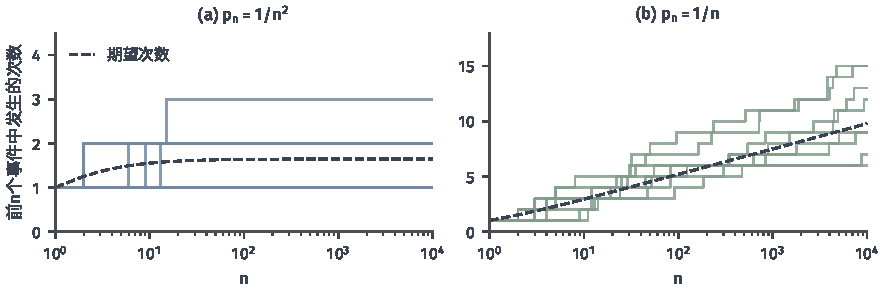
\includegraphics[width=150mm]{figures/02-abstract-mathematics/02-probability-spaces/matplotlib/conv-borel-cantelli/figure.pdf}
  \caption{独立事件发生次数的模拟，横轴为对数刻度。每个面板用固定随机种子画出$8$条路径，纵轴为$A_1,\ldots,A_n$中发生的个数，虚线为其期望$\sum_{k\leq n}\mathbb P(A_k)$。(a) $\mathbb P(A_n)=1/n^2$，各路径在$n=10^4$时的次数为$1$到$3$；(b) $\mathbb P(A_n)=1/n$，次数为$6$到$15$且仍在增长。}
  \label{fig:conv-borel-cantelli}
\end{figure*}

\subsection{依概率收敛的子列判据}

\paragraph{抽取几乎处处收敛的子列}
二进区间扫描整列不几乎处处收敛，但如果只看一部分项呢？
取$n_k=2^k$，即每一轮的第一项，$X_{2^k}=\mathbb I_{\{U<2^{-k}\}}$。
对每个$u>0$，一旦$2^{-k}\leq u$，此后这个子列就恒为$0$；所以这个子列几乎处处收敛到$0$。
关键在于：这个子列的坏事件概率$2^{-k}$可求和，而整列的坏事件概率在每一轮中加起来都是$1$，总和发散。
这启发我们，从任何依概率收敛的序列中，都可以挑出坏事件概率可求和的一个子列，再用Borel--Cantelli引理。

\begin{theorem}[依概率收敛的子列判据]
\label{thm:conv-subsequence}
$X_n\xrightarrow{\mathbb P}X$，当且仅当$(X_n)$的每个子列$(X_{n_j})$都有进一步的子列$(X_{n_{j_k}})$满足$X_{n_{j_k}}\xrightarrow{\mathrm{a.s.}}X$。
特别地，若$X_n\xrightarrow{\mathbb P}X$，则存在子列$X_{n_k}\xrightarrow{\mathrm{a.s.}}X$。
\end{theorem}

\begin{proof}[必要性]
设$X_n\xrightarrow{\mathbb P}X$，$(X_{n_j})$是任一子列，它同样依概率收敛于$X$。
对$k=1,2,\ldots$依次选取$j_k>j_{k-1}$，使
\[
  \mathbb P\bigl(|X_{n_{j_k}}-X|>2^{-k}\bigr)\leq2^{-k};
\]
这是可以做到的，因为对固定的$k$，左侧的概率随$j\to\infty$趋于零。
记$B_k=\{|X_{n_{j_k}}-X|>2^{-k}\}$，则$\sum_k\mathbb P(B_k)\leq\sum_k2^{-k}=1<\infty$。
由引理~\ref{lem:conv-borel-cantelli}第一部分，几乎每个$\omega$只属于有限多个$B_k$，即存在依赖于$\omega$的$K$，使$k\geq K$时$|X_{n_{j_k}}(\omega)-X(\omega)|\leq2^{-k}$。
于是这些$\omega$上$X_{n_{j_k}}(\omega)\to X(\omega)$。
\end{proof}

证明中阈值和概率同时取$2^{-k}$。阈值趋于零保证最终误差变小；概率可求和保证坏事件只发生有限次。
图~\ref{fig:conv-subsequence}在二进区间扫描上显示了这一区别。
左图中，样本$u=0.3$的全序列每轮都有一个$1$，而方框标出的子列$n_k=2^k$在$k\geq2$后恒为$0$；右图比较两者坏事件概率的累计和，全序列每轮增加$1$，子列的累计和不超过$2$。
子列是事先确定的下标序列，不随$\omega$改变；对每一个这样选定的子列，Borel--Cantelli引理保证几乎所有样本结果最终都避开坏事件。

\begin{figure*}[htbp]
  \centering
  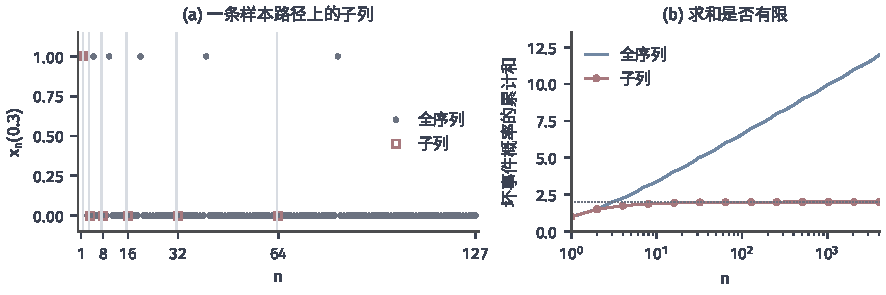
\includegraphics[width=150mm]{figures/02-abstract-mathematics/02-probability-spaces/matplotlib/conv-subsequence/figure.pdf}
  \caption{二进区间扫描中的子列抽取。(a) 样本$u=0.3$的全序列$X_n(0.3)$（灰点，$n\leq127$）与子列$n_k=2^k$（红色方框），竖线为各轮起点；(b) 坏事件概率$\mathbb P(X_n=1)$的累计和，横轴为对数刻度：全序列每轮增加$1$，到$n=2^{12}$约为$12$；子列$\sum_k2^{-k}$的累计和趋于$2$（点线）。}
  \label{fig:conv-subsequence}
\end{figure*}

\paragraph{充分性与反证}
反过来，如果每个子列都能再抽出几乎处处收敛到$X$的子列，原序列是否依概率收敛？

\begin{proof}[充分性]
若$X_n\xrightarrow{\mathbb P}X$不成立，则存在$\varepsilon>0$，使$\mathbb P(|X_n-X|>\varepsilon)$不趋于$0$；于是又存在$\delta>0$及子列$(n_j)$，使
\[
  \mathbb P\bigl(|X_{n_j}-X|>\varepsilon\bigr)\geq\delta\quad\text{对所有}j\text{成立}.
\]
按假设，$(X_{n_j})$有进一步的子列$X_{n_{j_k}}\xrightarrow{\mathrm{a.s.}}X$；由定理~\ref{thm:conv-implications}(1)，它也依概率收敛于$X$，故$\mathbb P(|X_{n_{j_k}}-X|>\varepsilon)\to0$，与上式中的下界$\delta$矛盾。
\end{proof}

判据要求的是“每个子列”都有进一步的子列收敛到\emph{同一个}$X$，只找到一个收敛子列是不够的。
令$X_n=0$（$n$为奇数），$X_n=1$（$n$为偶数），即在$0$与$1$之间交替的常数随机变量。
偶数项组成的子列收敛到$1$，奇数项组成的子列收敛到$0$；若$X_n\xrightarrow{\mathbb P}X$，两个子列也都依概率收敛于$X$，由极限唯一性$X$几乎必然既等于$1$又等于$0$，矛盾。所以这一列不依概率收敛。

子列判据的用处，是让依概率收敛可以借用那些需要几乎处处收敛作条件的定理。
例如，设$g:\mathbb R\to\mathbb R$连续，$X_n\xrightarrow{\mathbb P}X$。
任取子列，先抽出进一步的子列几乎处处收敛于$X$，由$g$的连续性，这个子列上$g(X_{n_{j_k}})\to g(X)$几乎处处成立；由判据的充分性，$g(X_n)\xrightarrow{\mathbb P}g(X)$。
下一节将以同样方式把控制收敛定理推广到依概率收敛。

\subsection{尾事件与零一律（补充）}

本小节补充独立序列的尾事件性质。
前面的子列判据和后面强大数律的证明都不依赖这里的结论，读者可以先跳过；但它解释了一个在后文反复出现的现象：随机级数是否收敛、样本平均是否收敛，这类问题的答案在独立情形下总是“几乎必然是”或“几乎必然不是”。

\paragraph{尾$\sigma$代数}
考察一列随机变量$X_1,X_2,\ldots$。
有些事件不受前面任何有限多项的影响。
例如级数$\sum_nX_n$是否收敛：去掉或改动前$m-1$项，部分和只差一个固定的有限数，收敛与否不变，所以这个事件可以只用$X_m,X_{m+1},\ldots$来判断。
又如样本平均$\bar X_n=\frac1n\sum_{k=1}^nX_k$是否收敛到给定常数$c$：由于$\frac1n\sum_{k<m}X_k\to0$对每个样本结果成立，$\bar X_n\to c$当且仅当$\frac1n\sum_{k=m}^nX_k\to c$，后者也只依赖$X_m,X_{m+1},\ldots$。
相反，“级数的和等于$1$”就不是这样的事件，因为改动$X_1$会改变和的值。

用$\sigma(X_m,X_{m+1},\ldots)$表示由$X_m,X_{m+1},\ldots$生成的$\sigma$代数，即使这些随机变量都可测的最小$\sigma$代数（第~\ref{chap:probability-models}章定义~\ref{def:pmod-generated-sigma}的推广）。

\begin{definition}[尾$\sigma$代数]
\label{def:conv-tail-sigma}
随机变量列$(X_n)$的\term{尾$\sigma$代数}（tail sigma-algebra）为
\[
  \mathcal T=\bigcap_{m=1}^{\infty}\sigma(X_m,X_{m+1},\ldots),
\]
其中的事件称为\term{尾事件}（tail event）。
\end{definition}

上面两个例子中的事件对每个$m$都属于$\sigma(X_m,X_{m+1},\ldots)$：用式~\eqref{eq:conv-convergence-event}的写法把“收敛”展开为可数次交并，每一步只用到下标不小于$m$的变量。所以它们都是尾事件。

\paragraph{Kolmogorov零一律}
尾事件不受任何有限个初始变量影响。若各变量相互独立，尾事件就与任何有限个初始变量独立；而尾事件本身又由全部变量决定，下面的证明说明这迫使它与自己独立，即$\mathbb P(A)=\mathbb P(A)^2$。

\begin{theorem}[Kolmogorov零一律]
\label{thm:conv-zero-one}
设$X_1,X_2,\ldots$相互独立，$\mathcal T$是它们的尾$\sigma$代数，则每个$A\in\mathcal T$都满足$\mathbb P(A)=0$或$\mathbb P(A)=1$。
\end{theorem}

这一结论称为\term{Kolmogorov零一律}（Kolmogorov zero-one law）。证明的思路是把尾事件与越来越长的初始段比较。

\begin{proof}
记$\mathcal F_n=\sigma(X_1,\ldots,X_n)$。
按第~\ref{chap:probability-models}章定理~\ref{thm:pmod-independence-grouping}，独立变量分成不相交的两组后，两组生成的$\sigma$代数仍独立，所以$\mathcal F_n$与$\sigma(X_{n+1},X_{n+2},\ldots)$独立；$\mathcal T$包含于后者，故$\mathcal F_n$与$\mathcal T$独立。

固定$A\in\mathcal T$。在$\mathcal F_\infty=\sigma(X_1,X_2,\ldots)$上定义两个有限测度$\mu(B)=\mathbb P(B\cap A)$与$\nu(B)=\mathbb P(B)\mathbb P(A)$。
集合族$\mathcal C=\bigcup_n\mathcal F_n$包含$\Omega$，对有限交封闭（$\mathcal F_n$递增，两个集合总落在同一个$\mathcal F_n$中），并生成$\mathcal F_\infty$；上一段说明$\mu=\nu$在$\mathcal C$上成立。
由第~\ref{chap:measures}章定理~\ref{thm:measure-uniqueness}，$\mu=\nu$在整个$\mathcal F_\infty$上成立。
$A$本身属于$\mathcal T\subseteq\mathcal F_\infty$，取$B=A$得$\mathbb P(A)=\mathbb P(A)^2$，所以$\mathbb P(A)\in\{0,1\}$。
\end{proof}

于是对独立的$X_n$，随机级数$\sum_nX_n$几乎必然收敛或几乎必然发散，样本平均几乎必然收敛到$c$或几乎必然不收敛到$c$，没有中间情形。
零一律只说概率是$0$或$1$，并不告诉我们是哪一个。
要判断某个随机级数确实收敛，仍需要第~\ref{sec:conv-partial-sums}节的方差估计；要判断样本平均确实收敛到均值，仍需要第~\ref{sec:conv-sample-means}节的证明。
所以零一律不能代替强大数律的证明，它的作用是说明那里得到的“几乎必然”结论不是偶然的。

\section{随机变量列的期望极限}
\label{sec:conv-expectation-limits}

本节研究$X_n$趋于$X$之后，期望$\mathbb EX_n$是否趋于$\mathbb EX$，以及平均误差$\mathbb E|X_n-X|^p$是否趋于零。
这里的期望是对底层概率测度$\mathbb P$的积分：固定$n$时，$\mathbb EX_n$是一个确定的数，而不是把前$n$个观测相加再除以$n$得到的样本平均，后者是第~\ref{sec:conv-sample-means}节的对象。
尖峰例子已经表明，几乎处处收敛本身不足以让极限进入期望。
我们先用已有的可积控制条件处理这个问题，并借助子列判据把它推广到依概率收敛；再从尖峰的失效机制中提炼出一致可积，最后证明它恰好刻画了依概率收敛何时升级为一阶平均收敛。

\subsection{有界与可积控制下的期望极限}

\paragraph{共同的可积上界}
尖峰缺少的是什么？
若存在一个随机变量$Y$同时控制所有$X_n=n\,\mathbb I_{\{0<U<1/n\}}$，它在$U=u\in(0,1)$处至少要达到$\sup_nX_n(u)$，即小于$1/u$的最大正整数，这个数不小于$1/u-1$；而$\mathbb E(1/U)=\int_0^1u^{-1}\,du=\infty$。
所以尖峰没有可积的共同上界，越来越高的峰合起来的“包络”面积是无穷大。

有了共同的可积上界，情况就不同了。
设$X_n\xrightarrow{\mathrm{a.s.}}X$，且存在$Y\geq0$，$\mathbb EY<\infty$，使每个$n$都有$|X_n|\leq Y$几乎必然成立。
可数个“$|X_n|\leq Y$”的例外事件与不收敛事件合并后仍是零概率事件，在其外取极限得$|X|\leq Y$，于是$|X_n-X|\leq2Y$。
对$|X_n-X|\to0$应用控制收敛定理（定理~\ref{thm:integral-dominated-convergence}），控制函数为$2Y$，得$\mathbb E|X_n-X|\to0$；再由
\[
  |\mathbb EX_n-\mathbb EX|=|\mathbb E(X_n-X)|\leq\mathbb E|X_n-X|
\]
得到$\mathbb EX_n\to\mathbb EX$。
$Y$取常数$c$时就是有界收敛：一列一致有界、几乎处处收敛的随机变量，其期望也收敛。
这里没有重新证明控制收敛定理，只是把它的条件翻译成概率语言：几乎处处收敛对应几乎处处的逐点收敛，共同上界对应可积控制函数。

\paragraph{依概率收敛下的控制收敛}
控制收敛定理要求逐点（几乎处处）收敛。
若只知道依概率收敛，就不能直接调用它；但子列判据允许我们先在子列上使用它，再回到整列。

\begin{theorem}[依概率收敛下的控制收敛]
\label{thm:conv-dominated-probability}
设$X_n\xrightarrow{\mathbb P}X$，且存在随机变量$Y\geq0$，$\mathbb EY<\infty$，使每个$n$都有$|X_n|\leq Y$几乎必然成立。
则$|X|\leq Y$几乎必然成立，$\mathbb E|X_n-X|\to0$，从而$\mathbb EX_n\to\mathbb EX$。
\end{theorem}

\begin{proof}
由定理~\ref{thm:conv-subsequence}，存在子列$X_{n_k}\xrightarrow{\mathrm{a.s.}}X$。在概率为$1$的事件上同时有$X_{n_k}\to X$与$|X_{n_k}|\leq Y$对所有$k$成立，取极限得$|X|\leq Y$几乎必然成立。

再证$\mathbb E|X_n-X|\to0$。若不然，存在$\delta>0$及子列$(n_j)$使$\mathbb E|X_{n_j}-X|\geq\delta$对所有$j$成立。
子列$(X_{n_j})$仍依概率收敛于$X$，再由定理~\ref{thm:conv-subsequence}抽出进一步的子列$X_{n_{j_k}}\xrightarrow{\mathrm{a.s.}}X$。
在这个子列上$|X_{n_{j_k}}-X|\leq2Y$几乎必然成立，由控制收敛定理$\mathbb E|X_{n_{j_k}}-X|\to0$，与下界$\delta$矛盾。
期望的收敛由$|\mathbb EX_n-\mathbb EX|\leq\mathbb E|X_n-X|$得到。
\end{proof}

证明中子列论证用了两次：一次得到极限的上界，一次把“整列不收敛”转化为“某个子列一直远离”，再与进一步子列上的控制收敛相矛盾。
依概率收敛本身不是控制收敛定理的条件；起作用的是子列判据提供的几乎处处收敛子列。

\begin{example}[有界函数的期望]
\label{ex:conv-bounded-function}
设估计量$\hat\theta_n\xrightarrow{\mathbb P}\theta$，$\theta$是常数，$g$是有界连续函数，$|g|\leq c$。
由上一节用子列判据得到的连续映射结论，$g(\hat\theta_n)\xrightarrow{\mathbb P}g(\theta)$；取$Y=c$，定理~\ref{thm:conv-dominated-probability}给出$\mathbb Eg(\hat\theta_n)\to g(\theta)$。
有界性不能去掉：令$\hat\theta_n=\theta+n\,\mathbb I_{\{0<U<1/n\}}$，取$g(t)=t$，则$\hat\theta_n\xrightarrow{\mathbb P}\theta$，但$\mathbb E\hat\theta_n=\theta+1$。
\end{example}

\subsection{一致可积的定义与判别}

\paragraph{尖峰把积分推向越来越小的事件}
共同的可积上界是充分条件，但要求太强。
例如对$n\geq3$令$X_n=\frac{n}{\ln n}\,\mathbb I_{\{0<U<1/n\}}$，它几乎处处趋于$0$，期望$1/\ln n$也趋于$0$；但$\sup_nX_n(u)$在$u$接近$0$时约为$\frac{1}{u\ln(1/u)}$，而$\int_0^{1/3}\frac{du}{u\ln(1/u)}=\infty$，所以它没有可积的共同上界。
这说明需要一个比共同上界更贴近问题的条件。

为此回到尖峰，找出它失效的确切原因。
对阈值$K\geq1$，$X_n=n\,\mathbb I_{\{0<U<1/n\}}$在$n\leq K$时从不超过$K$，在$n>K$时只要非零就超过$K$，所以
\[
  \mathbb E\bigl[X_n\,\mathbb I_{\{X_n>K\}}\bigr]=
  \begin{cases}0,&n\leq K,\\ 1,&n>K.\end{cases}
\]
对每个固定的$n$，这个尾部积分在$K\geq n$后变为$0$；但无论$K$多大，总有$n>K$的项把全部积分$1$放在阈值以上。
期望不随几乎处处极限变化，正是因为越来越小的事件仍携带固定大小的积分。
要排除这种现象，需要一个阈值同时控制整个序列的尾部积分。

\begin{definition}[一致可积]
\label{def:conv-uniform-integrability}
设$\{X_i:i\in I\}$是一族可积随机变量，$I$为任意指标集。若
\[
  \lim_{K\to\infty}\sup_{i\in I}\mathbb E\bigl[|X_i|\,\mathbb I_{\{|X_i|>K\}}\bigr]=0,
\]
则称这族随机变量\term{一致可积}（uniformly integrable）。
\end{definition}

“一致”指同一个$K$对全族有效。
单个可积随机变量$X$的尾部积分$\mathbb E[|X|\,\mathbb I_{\{|X|>K\}}]$随$K\to\infty$趋于$0$：被积函数几乎处处趋于$0$，且受$|X|$控制，由控制收敛定理即得。对有限族，上确界只是有限个趋于$0$的量取最大，所以有限族总是一致可积的。
尖峰说明可数族未必如此：每一项分别可积，尾部积分对每项分别趋于零，但上确界恒为$1$。

\paragraph{一致可积的判别}
直接验证定义往往不方便。下面的判别把一致可积与更容易检查的矩条件或控制条件联系起来。

\begin{theorem}[一致可积的判别]
\label{thm:conv-ui-criteria}
设$\{X_i:i\in I\}$是一族可积随机变量。
\begin{enumerate}
  \item 若这族一致可积，则$\sup_{i}\mathbb E|X_i|<\infty$。
  \item 若存在$Y\geq0$，$\mathbb EY<\infty$，使$|X_i|\leq Y$几乎必然对每个$i$成立，则这族一致可积。
  \item 若存在$r>1$使$C=\sup_i\mathbb E|X_i|^r<\infty$，则这族一致可积，且$\sup_i\mathbb E[|X_i|\,\mathbb I_{\{|X_i|>K\}}]\leq CK^{1-r}$。
  \item 若$A_i,B_i\geq0$，$0\leq W_i\leq A_i+B_i$，而$\{A_i\}$与$\{B_i\}$都一致可积，则$\{W_i\}$一致可积。
\end{enumerate}
\end{theorem}

\begin{proof}
(1) 取$K_0$使$\sup_i\mathbb E[|X_i|\,\mathbb I_{\{|X_i|>K_0\}}]\leq1$。把$|X_i|$按是否超过$K_0$拆开，
\[
  \mathbb E|X_i|=\mathbb E\bigl[|X_i|\,\mathbb I_{\{|X_i|\leq K_0\}}\bigr]+\mathbb E\bigl[|X_i|\,\mathbb I_{\{|X_i|>K_0\}}\bigr]\leq K_0+1.
\]

(2) $\{|X_i|>K\}\subseteq\{Y>K\}$且$|X_i|\leq Y$，所以$\mathbb E[|X_i|\,\mathbb I_{\{|X_i|>K\}}]\leq\mathbb E[Y\,\mathbb I_{\{Y>K\}}]$，右侧与$i$无关，且由单个可积变量的结论趋于$0$。

(3) 在事件$\{|X_i|>K\}$上，$|X_i|=|X_i|^r\cdot|X_i|^{1-r}\leq|X_i|^rK^{1-r}$，因为$1-r<0$。取期望得$\mathbb E[|X_i|\,\mathbb I_{\{|X_i|>K\}}]\leq K^{1-r}\mathbb E|X_i|^r\leq CK^{1-r}$。

(4) 在$\{A_i+B_i>K\}$上，$A_i,B_i$中较大者超过$K/2$，所以
\[
  W_i\,\mathbb I_{\{W_i>K\}}\leq(A_i+B_i)\,\mathbb I_{\{A_i+B_i>K\}}\leq2A_i\,\mathbb I_{\{A_i>K/2\}}+2B_i\,\mathbb I_{\{B_i>K/2\}},
\]
第一个不等号用了$W_i\leq A_i+B_i$与$\{W_i>K\}\subseteq\{A_i+B_i>K\}$。取期望再对$i$取上确界，右侧随$K\to\infty$趋于$0$。
\end{proof}

结论(1)的逆命题不成立：尖峰满足$\sup_n\mathbb E|X_n|=1$，却不一致可积。
一阶矩有界只限制了每项积分的总量，没有限制这份积分能被挤到多么稀有的事件上；结论(3)要求高于一阶的矩有界，正是对这种挤压的惩罚。
另一方面，一致可积也严格弱于结论(2)的共同控制。
前面没有可积上界的$X_n=\frac{n}{\ln n}\,\mathbb I_{\{0<U<1/n\}}$（$n\geq3$）在$X_n>K$时取值$n/\ln n$，尾部积分等于$\frac{n}{\ln n}\cdot\frac1n=\frac1{\ln n}$，否则为$0$；对$K\geq3$，$n/\ln n>K$迫使$n>K$，所以尾部积分的上确界不超过$1/\ln K\to0$，这族一致可积。

图~\ref{fig:conv-ui-tails}比较了两族随机变量。
尖峰族的尾部积分上确界对所有$K$都等于$1$；把峰高从$n$降为$\sqrt n$，得到$X_n=\sqrt n\,\mathbb I_{\{0<U<1/n\}}$，它满足$\mathbb EX_n^2=1$，由结论(3)取$r=2$，尾部积分上确界不超过$1/K$。
图中右栏显示尖峰族逐项的尾部积分：每条曲线在$K=n$处降到$0$，但$n$越大降得越晚，没有一个$K$能让所有曲线都降下来。

\begin{figure*}[htbp]
  \centering
  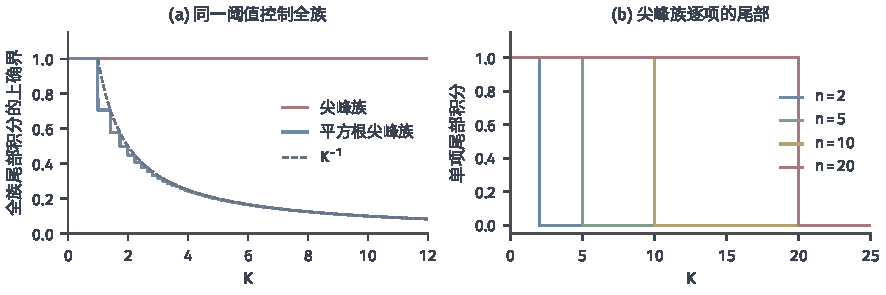
\includegraphics[width=150mm]{figures/02-abstract-mathematics/02-probability-spaces/matplotlib/conv-ui-tails/figure.pdf}
  \caption{尾部积分与一致可积，$U\sim\mathrm{Unif}[0,1)$。(a) $\sup_n\mathbb E[X_n\,\mathbb I_{\{X_n>K\}}]$随$K$的变化：尖峰族$X_n=n\,\mathbb I_{\{0<U<1/n\}}$恒为$1$；平方根尖峰族$X_n=\sqrt n\,\mathbb I_{\{0<U<1/n\}}$的精确值为$(\lfloor K^2\rfloor+1)^{-1/2}$，虚线为二阶矩给出的上界$1/K$。(b) 尖峰族中$n=2,5,10,20$各项的尾部积分$\mathbb E[X_n\,\mathbb I_{\{X_n>K\}}]=\mathbb I_{\{n>K\}}$。}
  \label{fig:conv-ui-tails}
\end{figure*}

\subsection{一致可积条件下的平均收敛}

\paragraph{一致可积与一阶平均收敛}
现在可以回答本节开头的问题：在依概率收敛的前提下，什么条件恰好保证平均误差趋于零？

\begin{theorem}[一致可积与一阶平均收敛]
\label{thm:conv-ui-l1}
设每个$X_n$可积，且$X_n\xrightarrow{\mathbb P}X$。则下列两条等价：
\begin{enumerate}
  \item $\{X_n\}$一致可积；
  \item $X$可积，且$\mathbb E|X_n-X|\to0$。
\end{enumerate}
此时$\mathbb EX_n\to\mathbb EX$。
\end{theorem}

\begin{proof}
(1)$\Rightarrow$(2)。先证$X$可积。取子列$X_{n_k}\xrightarrow{\mathrm{a.s.}}X$，由Fatou引理（引理~\ref{lem:integral-fatou}）与定理~\ref{thm:conv-ui-criteria}(1)，
\[
  \mathbb E|X|\leq\liminf_{k\to\infty}\mathbb E|X_{n_{k}}|\leq\sup_n\mathbb E|X_n|<\infty.
\]
再把误差分成有界部分和大值尾部。对$K>0$，令
\[
  \varphi_K(x)=\max\{-K,\min\{x,K\}\},
\]
它把$x$截到$[-K,K]$中，满足$|\varphi_K(x)-\varphi_K(y)|\leq|x-y|$与$|x-\varphi_K(x)|\leq|x|\,\mathbb I_{\{|x|>K\}}$。由三角不等式，
\[
  |X_n-X|\leq|\varphi_K(X_n)-\varphi_K(X)|+|X_n|\,\mathbb I_{\{|X_n|>K\}}+|X|\,\mathbb I_{\{|X|>K\}}.
\]
第一项满足$|\varphi_K(X_n)-\varphi_K(X)|\leq|X_n-X|$，所以$\varphi_K(X_n)\xrightarrow{\mathbb P}\varphi_K(X)$，且它们都以常数$K$为界；由定理~\ref{thm:conv-dominated-probability}，第一项的期望趋于$0$。于是
\[
  \limsup_{n\to\infty}\mathbb E|X_n-X|\leq\sup_n\mathbb E\bigl[|X_n|\,\mathbb I_{\{|X_n|>K\}}\bigr]+\mathbb E\bigl[|X|\,\mathbb I_{\{|X|>K\}}\bigr].
\]
左侧与$K$无关；令$K\to\infty$，右侧第一项由一致可积趋于$0$，第二项由$X$可积趋于$0$。

(2)$\Rightarrow$(1)。固定$\eta>0$，取$N$使$n>N$时$\mathbb E|X_n-X|<\eta$。
先看$n>N$的项。由$|X_n|\leq|X_n-X|+|X|$，
\[
  \mathbb E\bigl[|X_n|\,\mathbb I_{\{|X_n|>K\}}\bigr]\leq\mathbb E|X_n-X|+\mathbb E\bigl[|X|\,\mathbb I_{\{|X_n|>K\}}\bigr].
\]
对最后一项，按$|X|$是否超过另一个阈值$M$拆开，并用Markov不等式，
\[
  \begin{aligned}
  \mathbb E\bigl[|X|\,\mathbb I_{\{|X_n|>K\}}\bigr]
  &\leq\mathbb E\bigl[|X|\,\mathbb I_{\{|X|>M\}}\bigr]+M\,\mathbb P(|X_n|>K)\\
  &\leq\mathbb E\bigl[|X|\,\mathbb I_{\{|X|>M\}}\bigr]+\frac{M\,L}{K},
  \end{aligned}
\]
其中$L=\sup_n\mathbb E|X_n|\leq\max_{n\leq N}\mathbb E|X_n|+\eta+\mathbb E|X|<\infty$。
先取$M$使$\mathbb E[|X|\,\mathbb I_{\{|X|>M\}}]<\eta$，再取$K$使$ML/K<\eta$，则所有$n>N$的尾部积分都小于$3\eta$。
剩下的$X_1,\ldots,X_N$是有限个可积变量，把$K$再取大一些，它们的尾部积分也都小于$\eta$。
所以当$K$充分大时$\sup_n\mathbb E[|X_n|\,\mathbb I_{\{|X_n|>K\}}]\leq3\eta$，由$\eta$的任意性，$\{X_n\}$一致可积。

最后，$|\mathbb EX_n-\mathbb EX|\leq\mathbb E|X_n-X|\to0$。
\end{proof}

在这个定理中，期望收敛是结论，而不是条件的替代品。
只知道有符号的期望收敛，并不能推出平均误差趋于零。
例如对$n\geq2$令$Z_n=n\,\mathbb I_{\{0<U<1/n\}}-n\,\mathbb I_{\{1/n\leq U<2/n\}}$：正、负两个尖峰在期望中相互抵消，$\mathbb EZ_n=0$，而且$Z_n\xrightarrow{\mathrm{a.s.}}0$，但$\mathbb E|Z_n|=2$。
平均误差同时累计两个尖峰的幅度，有符号的期望却看不到它们。

\paragraph{$p$阶平均收敛的条件}
同样的尾部控制可以用于$|X_n|^p$，从而处理$p$阶平均误差。

\begin{theorem}[$p$阶平均收敛的一致可积条件]
\label{thm:conv-ui-lp}
设$1\leq p<\infty$，每个$X_n$有有限$p$阶矩，$X_n\xrightarrow{\mathbb P}X$，且$\{|X_n|^p\}$一致可积。则$\mathbb E|X|^p<\infty$，并且$X_n\xrightarrow{L^p}X$。
特别地，若存在$\delta>0$使$\sup_n\mathbb E|X_n|^{p+\delta}<\infty$，则上述条件成立。
\end{theorem}

\begin{proof}
取子列$X_{n_k}\xrightarrow{\mathrm{a.s.}}X$，由Fatou引理及定理~\ref{thm:conv-ui-criteria}(1)，$\mathbb E|X|^p\leq\liminf_k\mathbb E|X_{n_k}|^p\leq\sup_n\mathbb E|X_n|^p<\infty$。
令$W_n=|X_n-X|^p$。由$t\mapsto t^p$的凸性，$W_n\leq2^{p-1}|X_n|^p+2^{p-1}|X|^p$；右侧第一族一致可积，第二项是单个可积变量，乘以常数$2^{p-1}$不改变一致可积性，所以由定理~\ref{thm:conv-ui-criteria}(4)，$\{W_n\}$一致可积。
又$\mathbb P(W_n>\varepsilon)=\mathbb P(|X_n-X|>\varepsilon^{1/p})\to0$，即$W_n\xrightarrow{\mathbb P}0$。对$W_n$应用定理~\ref{thm:conv-ui-l1}，得$\mathbb EW_n\to0$。
对充分条件，把定理~\ref{thm:conv-ui-criteria}(3)用于族$\{|X_n|^p\}$，取$r=(p+\delta)/p>1$，即得$\{|X_n|^p\}$一致可积。
\end{proof}

充分条件中的$\delta>0$不能取为$0$。
令$X_n=n^{1/p}\,\mathbb I_{\{0<U<1/n\}}$，则$\mathbb E|X_n|^p=1$对所有$n$成立，$p$阶矩统一有界；但$X_n\xrightarrow{\mathrm{a.s.}}0$，$\mathbb E|X_n-0|^p=1$，不$p$阶平均收敛。
统一有界的$p$阶矩是一致可积的必要条件，而不是充分条件；多出的$\delta$阶矩才把大值上的积分压下去。

\paragraph{固定信息下的条件期望}
平均收敛的一个直接用途，是把极限传入条件期望。
设$\mathcal G\subseteq\mathcal F$是固定的子$\sigma$代数，$X_n,X$可积。
第~\ref{chap:conditional-expectation}章证明了条件期望的线性性和收缩性（定理~\ref{thm:cond-rules}与定理~\ref{thm:cond-contraction}）：$\mathbb E[X_n\mid\mathcal G]-\mathbb E[X\mid\mathcal G]=\mathbb E[X_n-X\mid\mathcal G]$几乎必然成立，并且对可积的$Z$有$\mathbb E\bigl|\mathbb E[Z\mid\mathcal G]\bigr|\leq\mathbb E|Z|$。
取$Z=X_n-X$，得
\[
  \mathbb E\bigl|\mathbb E[X_n\mid\mathcal G]-\mathbb E[X\mid\mathcal G]\bigr|\leq\mathbb E|X_n-X|.
\]
所以只要$X_n\to X$一阶平均收敛，例如依概率收敛且一致可积，条件期望也一阶平均收敛，从而依概率收敛，并有几乎处处收敛的子列。

这一结论没有说整列条件期望几乎处处收敛。
若已知$X_n\xrightarrow{\mathrm{a.s.}}X$且有共同的可积上界，第~\ref{chap:conditional-expectation}章的条件控制收敛定理（定理~\ref{thm:cond-dominated}）给出几乎处处收敛；仅有平均收敛时则得不到：取$\mathcal G=\mathcal F$，条件期望就是$X_n$本身，而二进区间扫描一阶平均收敛却处处不收敛。

另一方面，缺少一致可积时，极限一般不能传入条件期望。
以尖峰$X_n=n\,\mathbb I_{\{0<U<1/n\}}$和$\mathcal G=\sigma(\mathbb I_{\{U<1/2\}})$为例：$n\geq2$时区间$(0,1/n)$落在$[0,1/2)$内，按“在$\mathcal G$的每一块上取平均”计算，$\mathbb E[X_n\mid\mathcal G]=2\,\mathbb I_{\{U<1/2\}}$，与$n$无关；而$X_n$的几乎处处极限$0$的条件期望是$0$。
本小节只讨论信息$\mathcal G$固定不变的情形；信息随$n$增加时条件期望的收敛属于鞅理论，留给卷三。

\section{部分和的收敛}
\label{sec:conv-partial-sums}

本节转向独立随机变量的部分和$S_n=\sum_{k=1}^nZ_k$。
随机级数$\sum_{k=1}^{\infty}Z_k$收敛，就是部分和序列$S_n$收敛；要判断它是否几乎处处收敛，需要知道$S_n$在整个过程中的波动，而不只是某个固定时刻的值。
我们先控制有限阶段内部分和的最大偏差，再由它得到方差可和条件下的随机级数收敛；最后用Kronecker引理把加权级数的收敛转化为平均值的收敛，为下一节的强大数律准备工具。

\subsection{独立部分和的最大偏差}

\paragraph{终点控制与全程控制}
设$Z_1,\ldots,Z_n$独立，$\mathbb EZ_i=0$，$\operatorname{Var}(Z_i)<\infty$。
独立变量的方差可加，所以$\operatorname{Var}(S_n)=\sum_{i=1}^n\operatorname{Var}(Z_i)$，Chebyshev不等式给出终点的偏差界$\mathbb P(|S_n|\geq a)\leq a^{-2}\sum_i\operatorname{Var}(Z_i)$。
可是$|S_n|$小，并不说明此前没有某个$|S_k|$越过阈值：部分和可以先冲出去再回来。
若对每个$k$分别用Chebyshev再相加，得到的是$a^{-2}\sum_{k=1}^n\operatorname{Var}(S_k)$；各项方差相同时，它约为终点界的$n/2$倍，$n$大时没有用处。
Kolmogorov发现，对独立中心化的和，全程最大偏差的概率与终点偏差满足同一个上界。

\begin{theorem}[Kolmogorov最大不等式]
\label{thm:conv-kolmogorov-maximal}
设$Z_1,\ldots,Z_n$相互独立，$\mathbb EZ_i=0$，$\mathbb EZ_i^2<\infty$，$S_k=\sum_{i=1}^kZ_i$。则对任意$a>0$，
\[
  \mathbb P\Bigl(\max_{1\leq k\leq n}|S_k|\geq a\Bigr)\leq\frac1{a^2}\sum_{i=1}^n\operatorname{Var}(Z_i).
\]
\end{theorem}

这个不等式称为\term{Kolmogorov最大不等式}（Kolmogorov's maximal inequality）。
它把$n$个时刻的坏事件$\{|S_1|\geq a\},\ldots,\{|S_n|\geq a\}$合并成一个事件，而概率上界没有变大。
图~\ref{fig:conv-kolmogorov-maximal}以$\pm1$等概率的步长为例，取$n=100$，此时$\sum_i\operatorname{Var}(Z_i)=100$。
左图中有三条路径在某个时刻达到了$|S_k|\geq12$，其中只有一条在终点仍满足$|S_{100}|\geq12$；右图用$20000$次模拟比较三条曲线，$a=12$时全程最大偏差的频率约为$0.47$，终点偏差约为$0.27$，而上界为$100/144\approx0.69$。
上界对全程最大偏差仍然成立，尽管全程最大偏差的概率明显大于终点偏差。

\begin{figure*}[htbp]
  \centering
  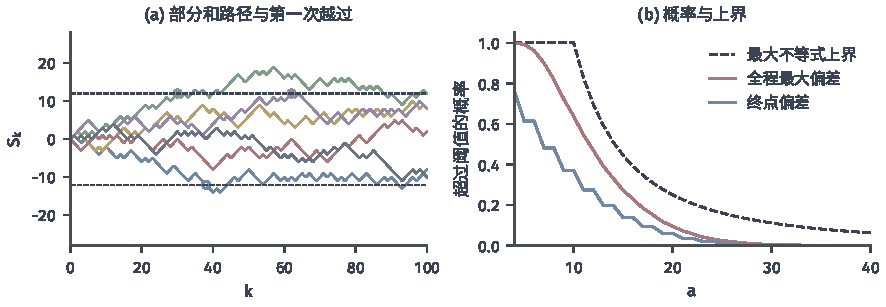
\includegraphics[width=150mm]{figures/02-abstract-mathematics/02-probability-spaces/matplotlib/conv-kolmogorov-maximal/figure.pdf}
  \caption{独立$\pm1$步长部分和的最大偏差，$n=100$。(a) 用固定随机种子画出的$6$条路径$S_k$，虚线为$\pm12$，空心圆标出各路径第一次满足$|S_k|\geq12$的位置；(b) $20000$次模拟中$\max_{k\leq100}|S_k|\geq a$（红）与$|S_{100}|\geq a$（蓝）的频率，虚线为最大不等式的上界$\min\{1,100/a^2\}$。终点曲线呈阶梯状，是因为$S_{100}$只取偶数值。}
  \label{fig:conv-kolmogorov-maximal}
\end{figure*}

\paragraph{按第一次越过的位置分解}
证明的想法是：把“曾经越过阈值”按\emph{第一次}越过的时刻分成互不相交的几种情形，在每种情形里，越过之后的增量与此前无关，平均起来不会把$S_n^2$拉小。

\begin{proof}
对$k=1,\ldots,n$，令
\[
  A_k=\bigl\{|S_k|\geq a,\ |S_j|<a\ \text{对所有}j<k\bigr\},
\]
即第一次越过阈值发生在时刻$k$。这些事件两两不交，并且$\bigcup_{k=1}^nA_k=\{\max_{k\leq n}|S_k|\geq a\}$。
记$R_k=S_n-S_k=\sum_{i=k+1}^nZ_i$为时刻$k$以后的增量。由于$\mathbb I_{A_k}\leq1$且两两不交，
\[
  \mathbb ES_n^2\geq\sum_{k=1}^n\mathbb E\bigl[S_n^2\,\mathbb I_{A_k}\bigr]
  =\sum_{k=1}^n\Bigl(\mathbb E\bigl[S_k^2\,\mathbb I_{A_k}\bigr]+2\,\mathbb E\bigl[S_k\mathbb I_{A_k}\cdot R_k\bigr]+\mathbb E\bigl[R_k^2\,\mathbb I_{A_k}\bigr]\Bigr).
\]
看中间的交叉项。$S_k\mathbb I_{A_k}$只依赖$Z_1,\ldots,Z_k$，$R_k$只依赖$Z_{k+1},\ldots,Z_n$；由第~\ref{chap:probability-models}章定理~\ref{thm:pmod-independence-grouping}，两组变量的函数相互独立。两者都有有限二阶矩，由Cauchy--Schwarz不等式（定理~\ref{thm:pmod-cauchy-schwarz}）其乘积可积，于是由定理~\ref{thm:pmod-product-expectation}，
\[
  \mathbb E\bigl[S_k\mathbb I_{A_k}\cdot R_k\bigr]=\mathbb E\bigl[S_k\mathbb I_{A_k}\bigr]\,\mathbb ER_k=0.
\]
第三项非负，舍去；在$A_k$上$S_k^2\geq a^2$。所以
\[
  \mathbb ES_n^2\geq\sum_{k=1}^n\mathbb E\bigl[S_k^2\,\mathbb I_{A_k}\bigr]\geq a^2\sum_{k=1}^n\mathbb P(A_k)=a^2\,\mathbb P\Bigl(\max_{1\leq k\leq n}|S_k|\geq a\Bigr).
\]
最后，$\mathbb ES_n^2=\operatorname{Var}(S_n)=\sum_i\operatorname{Var}(Z_i)$。
\end{proof}

整个证明只把一个事件分成了$n$个互不相交的事件；每个$A_k$由$Z_1,\ldots,Z_k$决定，而此后的增量$R_k$与它们独立且均值为零，这是交叉项消失的原因。
“第一次越过的时刻”是随机的，这一思想在卷三的停时与鞅理论中会得到系统发展，但这里不需要那些概念。

\subsection{方差可和条件下的级数收敛}

\paragraph{尾段的最大偏差}
现在考虑无穷多个独立、中心化的$Z_n$，问随机级数$\sum_nZ_n$何时几乎处处收敛。
\term{随机级数}（random series）收敛等价于部分和序列满足Cauchy条件，即足够晚以后任意两个部分和都很接近；这正是最大不等式能够控制的量。

\begin{theorem}[方差可和的独立级数]
\label{thm:conv-series}
设$Z_1,Z_2,\ldots$相互独立，$\mathbb EZ_n=0$，且$\sum_{n=1}^{\infty}\operatorname{Var}(Z_n)<\infty$。则$\sum_{n=1}^{\infty}Z_n$几乎处处收敛。
\end{theorem}

证明分两步。第一步把最大不等式用于从$m$开始的尾段。
对$m<j$，$S_k-S_m=\sum_{i=m+1}^kZ_i$（$m<k\leq j$）是独立中心化变量$Z_{m+1},\ldots,Z_j$的部分和，由定理~\ref{thm:conv-kolmogorov-maximal}，
\[
  \mathbb P\Bigl(\max_{m<k\leq j}|S_k-S_m|\geq\varepsilon\Bigr)\leq\frac1{\varepsilon^2}\sum_{i=m+1}^j\operatorname{Var}(Z_i)\leq\frac1{\varepsilon^2}\sum_{i>m}\operatorname{Var}(Z_i).
\]
若$\sup_{k>m}|S_k-S_m|>\varepsilon$，则存在某个$k$使$|S_k-S_m|>\varepsilon$，它属于$j=k$时左侧的事件。左侧事件随$j$递增，由概率的连续性，
\begin{equation}
  \mathbb P\Bigl(\sup_{k>m}|S_k-S_m|>\varepsilon\Bigr)\leq\frac1{\varepsilon^2}\sum_{i>m}\operatorname{Var}(Z_i).
  \label{eq:conv-tail-maximal}
\end{equation}
这个界同时控制了$m$以后\emph{所有}的部分和，而不只是某一个终点。

\paragraph{Cauchy条件与实数的完备性}
第二步把式~\eqref{eq:conv-tail-maximal}转化为Cauchy条件。

\begin{proof}[定理~\ref{thm:conv-series}的证明]
令$D_m=\sup_{k,l>m}|S_k-S_l|$，它衡量$m$以后部分和之间的最大差距。由三角不等式$|S_k-S_l|\leq|S_k-S_m|+|S_l-S_m|$，得$D_m\leq2\sup_{k>m}|S_k-S_m|$。
$D_m$随$m$递减，记其极限为$D=\lim_mD_m\in[0,\infty]$；对每个样本结果，部分和数列是Cauchy列当且仅当$D=0$。
对任意$\varepsilon>0$和任意$m$，$D\leq D_m$，所以由式~\eqref{eq:conv-tail-maximal}，
\[
  \mathbb P(D>2\varepsilon)\leq\mathbb P(D_m>2\varepsilon)\leq\mathbb P\Bigl(\sup_{k>m}|S_k-S_m|>\varepsilon\Bigr)\leq\frac1{\varepsilon^2}\sum_{i>m}\operatorname{Var}(Z_i).
\]
左侧与$m$无关，右侧是收敛级数的尾和，令$m\to\infty$得$\mathbb P(D>2\varepsilon)=0$。
取$\varepsilon=1/r$，$r=1,2,\ldots$，$\{D>0\}=\bigcup_r\{D>2/r\}$是可数个零概率事件之并，所以$D=0$几乎处处成立。
于是几乎每个样本结果上部分和都是实数的Cauchy列；由实数的完备性，它收敛。
\end{proof}

最后一步用的是每条样本路径上实数列的完备性：Cauchy数列必收敛。它与“平方可积随机变量构成完备空间”是不同的事实，后者属于第~\ref{part:function-spaces}部分，这里没有用到。
方差可和条件也蕴含$\mathbb E(S_n-S_m)^2=\sum_{i=m+1}^n\operatorname{Var}(Z_i)\to0$，即部分和的均方差距趋于零；但从均方差距到逐样本收敛，需要的正是最大不等式提供的全程控制。

\begin{example}[随机调和级数]
\label{ex:conv-random-harmonic}
设$\varepsilon_1,\varepsilon_2,\ldots$独立，各以概率$1/2$取$+1$和$-1$。
令$Z_n=\varepsilon_n/n$，则$\mathbb EZ_n=0$，$\sum_n\operatorname{Var}(Z_n)=\sum_n1/n^2=\pi^2/6<\infty$，由定理~\ref{thm:conv-series}，随机调和级数$\sum_n\varepsilon_n/n$几乎处处收敛。
普通的调和级数$\sum_n1/n$发散；随机符号使大部分项相互抵消，级数就收敛了。
更一般地，$\sum_n\varepsilon_n/n^{\alpha}$在$\alpha>1/2$时满足$\sum_nn^{-2\alpha}<\infty$，同样几乎处处收敛。
\end{example}

图~\ref{fig:conv-random-harmonic}左栏画出$\sum_{k\leq n}\varepsilon_k/k$的六条样本路径：每条路径在几百项以后几乎不再移动，但不同路径停在不同的值，极限本身是随机变量。
右栏是$\alpha=1/2$的临界情形$\sum_{k\leq n}\varepsilon_k/\sqrt k$，方差$\sum_{k\leq n}1/k$随$n$对数增长，定理~\ref{thm:conv-series}不适用；路径一直在游走，没有稳定下来。
事实上这个级数几乎处处发散，证明需要Kolmogorov三级数定理的必要性部分，本章不展开；由零一律（定理~\ref{thm:conv-zero-one}），它的收敛概率只能是$0$或$1$。

\begin{figure*}[htbp]
  \centering
  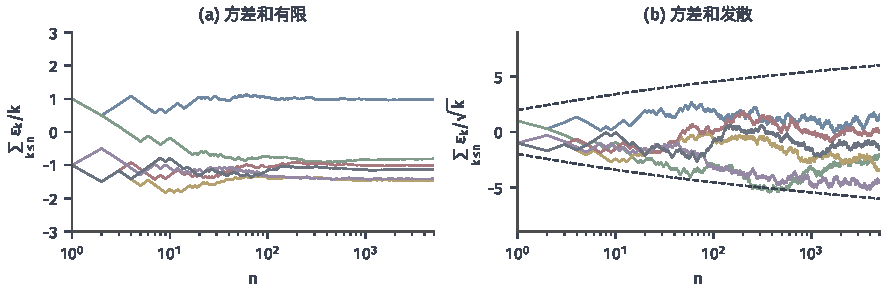
\includegraphics[width=150mm]{figures/02-abstract-mathematics/02-probability-spaces/matplotlib/conv-random-harmonic/figure.pdf}
  \caption{随机符号级数的部分和，$\varepsilon_k$独立且等概率取$\pm1$，横轴为对数刻度，用固定随机种子画出$6$条路径。(a) $\sum_{k\leq n}\varepsilon_k/k$，方差和为$\pi^2/6$，各路径在$n=5000$时分别停在约$-1.47$到$0.99$之间；(b) $\sum_{k\leq n}\varepsilon_k/\sqrt k$，虚线为$\pm2\bigl(\sum_{k\leq n}1/k\bigr)^{1/2}$，即两倍标准差。}
  \label{fig:conv-random-harmonic}
\end{figure*}

\subsection{由级数收敛得到平均值收敛}

\paragraph{Kronecker引理}
上一小节回答了级数何时收敛，而我们的最终目标是样本平均。
二者之间需要一个确定性的桥梁：若加权级数$\sum_nz_n/n$收敛，平均值$\frac1n\sum_{k=1}^nz_k$是否趋于零？
直觉是：$\sum z_n/n$收敛说明$z_n$的“累计贡献”增长得比$n$慢，所以除以$n$后消失。下面的\term{Kronecker引理}（Kronecker's lemma）用分部求和把这一直觉写成证明。

\begin{lemma}[Kronecker引理]
\label{lem:conv-kronecker}
设$z_1,z_2,\ldots$是实数，级数$\sum_{n=1}^{\infty}z_n/n$收敛。则
\[
  \lim_{n\to\infty}\frac1n\sum_{k=1}^nz_k=0.
\]
\end{lemma}

\begin{proof}
记$b_0=0$，$b_n=\sum_{k=1}^nz_k/k$，于是$z_k=k(b_k-b_{k-1})$，且$b_n\to b$为有限数。
用\term{Abel分部求和}（summation by parts）重新整理$\sum_{k=1}^nz_k$：
\[
  \sum_{k=1}^nk(b_k-b_{k-1})=\sum_{k=1}^nkb_k-\sum_{k=0}^{n-1}(k+1)b_k=nb_n-\sum_{k=1}^{n-1}b_k,
\]
最后一步把两个和中$k=1,\ldots,n-1$的项合并，$kb_k-(k+1)b_k=-b_k$，并用了$b_0=0$。两边除以$n$，
\begin{equation}
  \frac1n\sum_{k=1}^nz_k=b_n-\frac1n\sum_{k=1}^{n-1}b_k.
  \label{eq:conv-abel-identity}
\end{equation}
右侧第一项趋于$b$。第二项是$b_k$的\term{Cesàro平均}（Cesàro mean），也趋于$b$：对$\eta>0$取$N$使$k\geq N$时$|b_k-b|<\eta$，则当$n>N$时
\[
  \Bigl|\frac1n\sum_{k=1}^{n-1}b_k-b\Bigr|\leq\frac1n\sum_{k=1}^{N-1}|b_k-b|+\frac{n-N}{n}\,\eta+\frac{|b|}{n},
\]
右侧第一项和第三项的分子固定，随$n\to\infty$趋于$0$，所以上极限不超过$\eta$。
两项极限相同，相减得$0$。
\end{proof}

式~\eqref{eq:conv-abel-identity}是整个证明的核心：平均值等于加权部分和与它自身Cesàro平均的差，而一个收敛数列和它的Cesàro平均趋于同一极限。
图~\ref{fig:conv-kronecker}在随机调和级数的一条路径上画出了这三个量。
$b_n$在约$0.99$附近稳定下来，它的Cesàro平均以更平缓的方式追上它；两者之差就是$\varepsilon_k$的平均值，在$n=5000$时为$0.006$。

\begin{figure}[htbp]
  \centering
  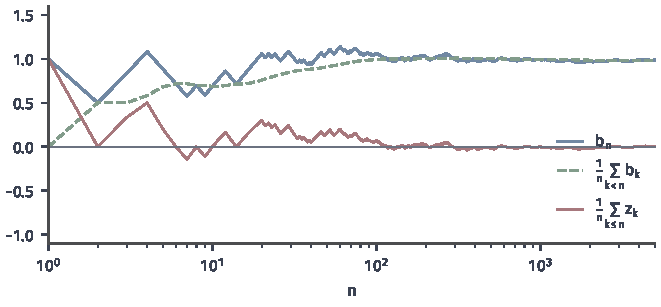
\includegraphics[width=112mm]{figures/02-abstract-mathematics/02-probability-spaces/matplotlib/conv-kronecker/figure.pdf}
  \caption{Kronecker引理中的恒等式~\eqref{eq:conv-abel-identity}，取$z_k=\varepsilon_k$为图~\ref{fig:conv-random-harmonic}(a)中第一条路径的随机符号，横轴为对数刻度。蓝线为$b_n=\sum_{k\leq n}z_k/k$，绿色虚线为其Cesàro平均$\frac1n\sum_{k<n}b_k$，红线为二者之差，即平均值$\frac1n\sum_{k\leq n}z_k$。}
  \label{fig:conv-kronecker}
\end{figure}

\begin{example}[确定性数列上的Kronecker引理]
\label{ex:conv-kronecker-deterministic}
取$z_k=(-1)^{k+1}\sqrt k$。级数$\sum_kz_k/k=\sum_k(-1)^{k+1}/\sqrt k$是交错级数，各项绝对值单调趋于零，所以收敛（其和约为$0.605$）。
由Kronecker引理，$\frac1n\sum_{k=1}^n(-1)^{k+1}\sqrt k\to0$；直接计算，$n=100$、$1000$、$10000$时这一平均值分别约为$-0.046$、$-0.015$、$-0.005$。
引理的逆命题不成立：$z_k=1/\ln(k+1)$满足$z_k\to0$，因而其Cesàro平均趋于$0$，但$\sum_k1/(k\ln(k+1))$发散。
\end{example}

\paragraph{逐个样本结果上的应用}
Kronecker引理是关于实数列的结论，用于随机变量时要逐个样本结果使用。
若存在概率为$1$的事件$E$，使每个$\omega\in E$上级数$\sum_nZ_n(\omega)/n$收敛，则对这些$\omega$都有$\frac1n\sum_{k=1}^nZ_k(\omega)\to0$，即$\frac1n\sum_{k=1}^nZ_k\xrightarrow{\mathrm{a.s.}}0$。
结合定理~\ref{thm:conv-series}，只需检验$Z_n/n$独立、中心化且$\sum_n\operatorname{Var}(Z_n)/n^2<\infty$。
这就是下一节的出发点。
引理还有一般的形式：若$0<a_n\uparrow\infty$且$\sum_nz_n/a_n$收敛，则$a_n^{-1}\sum_{k\leq n}z_k\to0$，证明方法相同；本章只用$a_n=n$的情形。

\section{样本平均的收敛}
\label{sec:conv-sample-means}

本节研究部分和按项数归一化后得到的样本平均$\bar X_n=\frac1n\sum_{k=1}^nX_k$。
我们回到章首的问题：卷一的弱大数律说$\bar X_n$偏离均值的概率趋于零，现在要证明更强的结论——几乎每条样本序列上$\bar X_n$都收敛到均值。
先说明为什么弱大数律的证明不能直接升级，再分两步证明：方差可和时直接用上一节的工具，只有一阶矩时用截断把问题化回方差可和的情形。

\subsection{从弱大数律到强大数律}

\paragraph{已有的弱大数律}
卷一已经证明：若$X_1,X_2,\ldots$独立同分布且$\mathbb E|X_1|<\infty$，则$\bar X_n\xrightarrow{\mathbb P}\mathbb EX_1$。
有限方差时那里用的是Chebyshev不等式；只有一阶矩时，那里先把每个观测在固定水平$M$处截断，用Markov不等式控制截断掉的尾部，再用Chebyshev控制有界部分。
本节不重复这些证明，而是讨论比它更强的结论。

\begin{definition}[强大数定律]
\label{def:conv-slln}
设随机变量列$(X_n)$的各项有相同的有限均值$\mu$。若$\bar X_n\xrightarrow{\mathrm{a.s.}}\mu$，称$(X_n)$满足\term{强大数定律}（strong law of large numbers），简称强大数律。
\end{definition}

“强”与“弱”的差别就是第~\ref{sec:conv-modes}节中几乎处处收敛与依概率收敛的差别。
由定理~\ref{thm:conv-implications}(1)，在相同条件下证明了强大数律，弱大数律就自动成立。
对章首的硬币问题，强大数律说的是：几乎每一次运行产生的频率序列，本身都收敛到$1/2$。

\paragraph{Chebyshev界为何不够}
设$X_n$独立同分布，方差$0<\sigma^2<\infty$，均值$\mu$。
Chebyshev不等式给出
\[
  \mathbb P(|\bar X_n-\mu|\geq\varepsilon)\leq\frac{\sigma^2}{n\varepsilon^2}.
\]
要用Borel--Cantelli引理得到几乎处处收敛，需要对每个$\varepsilon$这些概率可求和；但$\sum_n\sigma^2/(n\varepsilon^2)$是调和级数，发散。
所以不能把弱大数律的这一证明与Borel--Cantelli引理机械地连接起来。

图~\ref{fig:conv-chebyshev-nonsummable}以$\operatorname{Bernoulli}(1/2)$样本、$\varepsilon=0.1$为例做了比较。
Chebyshev上界是$\min\{1,25/n\}$；精确的误差概率由二项分布算出，$n=100$时约为$0.057$，$n=500$时约为$9\times10^{-6}$，下降远快于$1/n$。
右图中，精确概率的累计和到$n=2000$约为$26$且已停止增长，而上界的累计和约为$134$并按对数继续增长。
所以在这个例子里失效的是上界，不是事实本身：真实的误差概率是可求和的。
但只假设有限方差时，我们手中只有Chebyshev这样的二阶矩信息，必须找到不依赖指数小尾部的论证。

\begin{figure*}[htbp]
  \centering
  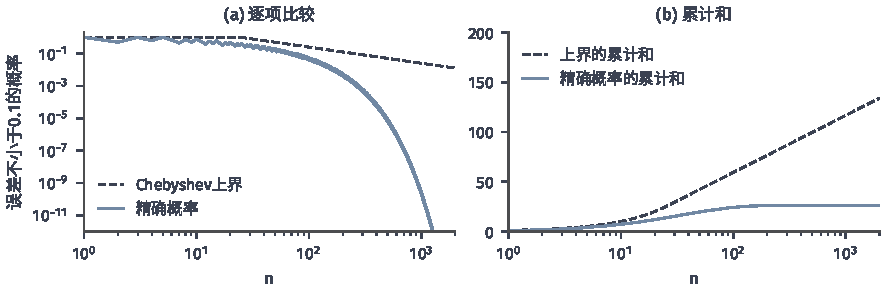
\includegraphics[width=150mm]{figures/02-abstract-mathematics/02-probability-spaces/matplotlib/conv-chebyshev-nonsummable/figure.pdf}
  \caption{$\operatorname{Bernoulli}(1/2)$样本平均的误差概率$\mathbb P(|\bar X_n-1/2|\geq0.1)$，横轴为对数刻度。(a) 精确值（由二项分布计算，蓝线）与Chebyshev上界$\min\{1,25/n\}$（虚线），纵轴为对数刻度；(b) 二者自$n=1$起的累计和，$n=2000$时分别约为$26.3$与$134.1$。}
  \label{fig:conv-chebyshev-nonsummable}
\end{figure*}

不过Chebyshev界并非毫无用处。
沿子列$n=m^2$，$\sum_m\sigma^2/(m^2\varepsilon^2)<\infty$，所以由Borel--Cantelli引理，$\bar X_{m^2}\xrightarrow{\mathrm{a.s.}}\mu$。
困难在于子列之间：$m^2$与$(m+1)^2$之间有$2m$项，需要控制$\bar X_n$在这一段中的全程波动。
这正是最大偏差的问题。第~\ref{sec:conv-partial-sums}节的最大不等式、级数收敛和Kronecker引理，提供了一条不经过子列、直接控制整条序列累计误差的路线。

\subsection{方差可和条件下的强大数律}

\paragraph{中心化后的加权级数}
把上一节的结论组合起来，先得到一个允许各项分布不同的版本。

\begin{theorem}[方差可和条件下的强大数律]
\label{thm:conv-slln-variance}
设$X_1,X_2,\ldots$相互独立，各有有限方差，且
\[
  \sum_{n=1}^{\infty}\frac{\operatorname{Var}(X_n)}{n^2}<\infty.
\]
则
\[
  \frac1n\sum_{k=1}^n\bigl(X_k-\mathbb EX_k\bigr)\xrightarrow{\mathrm{a.s.}}0.
\]
\end{theorem}

\begin{proof}
令$W_n=X_n-\mathbb EX_n$。变量$W_n/n$相互独立（各是$X_n$的函数），均值为零，方差$\operatorname{Var}(X_n)/n^2$可和。
由定理~\ref{thm:conv-series}，$\sum_nW_n/n$几乎处处收敛；在这个概率为$1$的事件上逐样本应用引理~\ref{lem:conv-kronecker}，得$\frac1n\sum_{k=1}^nW_k\to0$。
\end{proof}

这一结论不要求同分布，所得极限是减去各项期望之后的平均误差。
例如各批产品的合格率$p_n$不同，第$n$件是否合格记为$X_n\sim\operatorname{Bernoulli}(p_n)$，各件独立。
由于$\operatorname{Var}(X_n)=p_n(1-p_n)\leq1/4$，$\sum_n\operatorname{Var}(X_n)/n^2\leq\pi^2/24$，所以合格频率与平均合格率之差$\frac1n\sum_{k\leq n}(X_k-p_k)$几乎处处趋于零。
若$p_n$本身没有极限，合格频率也未必收敛，但它始终贴着$\frac1n\sum_{k\leq n}p_k$变化。

\paragraph{独立同分布且方差有限的情形}
独立同分布且方差$\sigma^2<\infty$时，$\sum_n\sigma^2/n^2<\infty$，定理~\ref{thm:conv-slln-variance}给出$\bar X_n\xrightarrow{\mathrm{a.s.}}\mu$。
同一条件下也有$\mathbb E(\bar X_n-\mu)^2=\sigma^2/n\to0$，即$\bar X_n\xrightarrow{L^2}\mu$。
两个结论都在“方差有限”下成立，但依据不同：均方收敛只需计算一个方差，几乎处处收敛还需要最大不等式对全程波动的控制。
二者互不蕴含，这在第~\ref{sec:conv-modes}节的反例中已经看到。

图~\ref{fig:conv-slln-paths}(a)画出均值为$1$的指数分布样本的五条平均值路径，它们在$n=10^5$时与$1$的距离都不超过$0.005$。
这一证明还没有覆盖只有有限一阶矩的样本：例如指数为$1.5$的Pareto分布有均值，方差却是无穷大，定理~\ref{thm:conv-slln-variance}的条件不满足。

\subsection{有限一阶矩条件下的强大数律}

\paragraph{定理与证明路线}
现在陈述本章的主要结论。

\begin{theorem}[强大数律]
\label{thm:conv-slln}
设$X_1,X_2,\ldots$独立同分布，$\mathbb E|X_1|<\infty$，$\mu=\mathbb EX_1$。则$\bar X_n\xrightarrow{\mathrm{a.s.}}\mu$。
\end{theorem}

条件中没有方差，所以不能直接用定理~\ref{thm:conv-slln-variance}。
办法与卷一的弱大数律类似，也是截断，但截断水平不再固定，而是随项数增长：令
\[
  Y_n=X_n\,\mathbb I_{\{|X_n|\leq n\}}.
\]
随$n$增大的截断水平带来三方面的结果，图~\ref{fig:conv-slln-roadmap}把它们和上一节的工具画在一起：截断改变的项只有有限个；截断项虽不同分布，却满足方差可和条件；截断项的期望仍趋于$\mu$。
下面三段依次证明这三点。

\begin{figure*}[htbp]
  \centering
  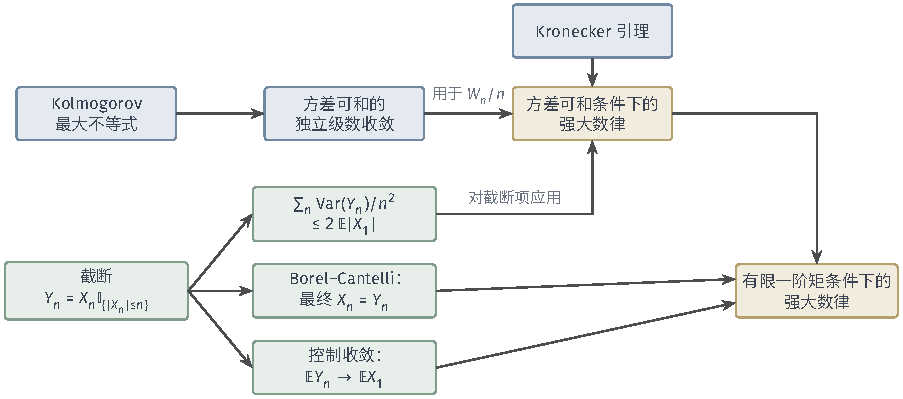
\includegraphics[width=153mm]{figures/02-abstract-mathematics/02-probability-spaces/tikz/conv-slln-roadmap/figure.pdf}
  \caption{强大数律的证明路线。蓝框是第~\ref{sec:conv-partial-sums}节的工具，绿框是截断$Y_n=X_n\mathbb I_{\{|X_n|\leq n\}}$带来的三步推导，黄框是两个层次的强大数律；箭头表示推导所用的依赖关系，$W_n=X_n-\mathbb EX_n$。}
  \label{fig:conv-slln-roadmap}
\end{figure*}

\paragraph{截断项与原序列最终一致}
由同分布，$\mathbb P(|X_n|>n)=\mathbb P(|X_1|>n)$。
对$t\in[n-1,n]$有$\mathbb P(|X_1|>n)\leq\mathbb P(|X_1|>t)$，所以
\[
  \begin{aligned}
  \sum_{n=1}^{\infty}\mathbb P(|X_n|>n)
  &\leq\sum_{n=1}^{\infty}\int_{n-1}^n\mathbb P(|X_1|>t)\,dt\\
  &=\int_0^{\infty}\mathbb P(|X_1|>t)\,dt=\mathbb E|X_1|<\infty.
  \end{aligned}
\]
最后一个等号是把$|X_1|=\int_0^{\infty}\mathbb I_{\{t<|X_1|\}}\,dt$代入期望，再对非负被积函数交换积分次序（定理~\ref{thm:analysis-tonelli-fubini}的Tonelli部分）。
由Borel--Cantelli引理第一部分，几乎必然只有有限个$n$满足$|X_n|>n$，即存在依赖于$\omega$的$N$，使$n\geq N$时$X_n=Y_n$。
于是$\sum_{k=1}^n(X_k-Y_k)$从某项起不再变化，是一个固定的有限数，除以$n$后趋于$0$：
\[
  \frac1n\sum_{k=1}^n(X_k-Y_k)\xrightarrow{\mathrm{a.s.}}0.
\]

图~\ref{fig:conv-truncation}以指数为$1.5$的Pareto分布为例。
它满足$\mathbb P(X_1>t)=t^{-1.5}$（$t\geq1$），均值为$3$，方差无穷大；被截断的项数的期望为$\sum_nn^{-1.5}\approx2.61$。
在所画的样本中，只有$n=1,3,11,93$四项超过了截断水平，此后再也没有；右图显示两种样本平均之差在$n=93$以后严格按“常数$/n$”衰减。

\begin{figure*}[htbp]
  \centering
  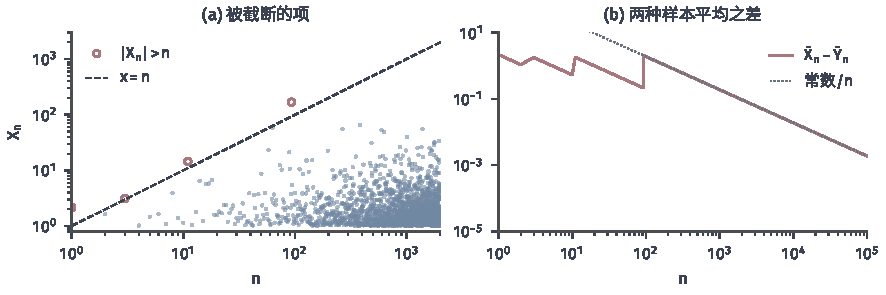
\includegraphics[width=150mm]{figures/02-abstract-mathematics/02-probability-spaces/matplotlib/conv-truncation/figure.pdf}
  \caption{截断$Y_n=X_n\mathbb I_{\{|X_n|\leq n\}}$与原序列的最终一致，$X_n$独立服从指数为$1.5$、下界为$1$的Pareto分布，固定随机种子。(a) 前$2000$个观测（双对数坐标），虚线为截断水平$x=n$，红圈为被截断的项，本样本中为$n=1,3,11,93$；(b) $\bar X_n-\bar Y_n$，$n\leq10^5$，点线为被截断部分的总和除以$n$。}
  \label{fig:conv-truncation}
\end{figure*}

\paragraph{截断项的方差可和}
截断项$Y_n$是独立的$X_n$各自的函数，所以仍相互独立，但截断水平随$n$变化，它们一般不再同分布。
每个$Y_n$以$n$为界，方差有限，且
\[
  \operatorname{Var}(Y_n)\leq\mathbb EY_n^2=\mathbb E\bigl[X_1^2\,\mathbb I_{\{|X_1|\leq n\}}\bigr],
\]
这里再次用了同分布。对非负项交换求和与期望（单调收敛定理），
\[
  \sum_{n=1}^{\infty}\frac{\operatorname{Var}(Y_n)}{n^2}\leq\mathbb E\Bigl[X_1^2\sum_{n\geq1,\ n\geq|X_1|}\frac1{n^2}\Bigr].
\]
现在估计内层的尾和。对正整数$m$，$\sum_{n\geq m}n^{-2}\leq m^{-2}+\int_m^{\infty}t^{-2}\,dt=m^{-2}+m^{-1}\leq2/m$。
若$|X_1|\geq1$，取$m=\lceil|X_1|\rceil\geq|X_1|$，内层和不超过$2/|X_1|$，乘以$X_1^2$后不超过$2|X_1|$；
若$|X_1|<1$，内层和是$\sum_{n\geq1}n^{-2}<2$，而$X_1^2\leq|X_1|$，乘积也不超过$2|X_1|$。
两种情形合起来得到
\[
  \sum_{n=1}^{\infty}\frac{\operatorname{Var}(Y_n)}{n^2}\leq2\,\mathbb E|X_1|<\infty.
\]
这是截断水平取$n$的关键：大的$|X_1|$只在$n\geq|X_1|$的项中出现，而这些项的权重$1/n^2$之和约为$1/|X_1|$，恰好把二阶量$X_1^2$降为一阶量$|X_1|$。
由定理~\ref{thm:conv-slln-variance}，
\[
  \frac1n\sum_{k=1}^n\bigl(Y_k-\mathbb EY_k\bigr)\xrightarrow{\mathrm{a.s.}}0.
\]

\paragraph{均值的恢复与三步合并}
还需说明截断项的期望趋于$\mu$。
由同分布，$\mathbb EY_n=\mathbb E[X_1\,\mathbb I_{\{|X_1|\leq n\}}]$。被积函数逐点趋于$X_1$，且以可积的$|X_1|$为界，由控制收敛定理，$\mathbb EY_n\to\mathbb EX_1=\mu$。
一个收敛数列的Cesàro平均趋于同一极限（这一点已在引理~\ref{lem:conv-kronecker}的证明中说明），所以$\frac1n\sum_{k=1}^n\mathbb EY_k\to\mu$。

把三步合在一起：
\[
  \bar X_n-\mu=\frac1n\sum_{k=1}^n(X_k-Y_k)+\frac1n\sum_{k=1}^n\bigl(Y_k-\mathbb EY_k\bigr)+\Bigl(\frac1n\sum_{k=1}^n\mathbb EY_k-\mu\Bigr).
\]
第一项由Borel--Cantelli引理几乎处处趋于$0$，第二项由方差可和的强大数律几乎处处趋于$0$，第三项是确定的数列，趋于$0$。
三个概率为$1$的事件之交仍有概率$1$，在其上$\bar X_n\to\mu$。定理~\ref{thm:conv-slln}得证。

一阶矩条件不能再去掉。
若$X_n$独立同分布而$\mathbb E|X_1|=\infty$，反方向的比较（对$t\in[n,n+1]$有$\mathbb P(|X_1|>n)\geq\mathbb P(|X_1|>t)$）给出$\sum_n\mathbb P(|X_n|>n)\geq\int_1^{\infty}\mathbb P(|X_1|>t)\,dt\geq\mathbb E|X_1|-1=\infty$；事件$\{|X_n|>n\}$相互独立，由Borel--Cantelli引理第二部分，几乎必然有无穷多个$n$满足$|X_n|>n$。
另一方面$X_n/n=\bar X_n-\frac{n-1}{n}\bar X_{n-1}$，若$\bar X_n$收敛到有限极限，右侧趋于$0$，与$|X_n|/n>1$无穷多次发生矛盾。
所以这时$\bar X_n$几乎必然不收敛到任何有限数。

图~\ref{fig:conv-slln-paths}对照了三种情形。
指数分布有有限方差，路径很快稳定；指数为$1.5$的Pareto分布只有一阶矩，路径时常被一个大观测拉开，但最终仍回到均值$3$附近，$n=10^5$时五条路径在$2.91$到$2.96$之间，收敛明显更慢；指数为$0.8$的Pareto分布没有均值，平均值被越来越大的观测不断推高，五条路径在$n=10^5$时散布在$60$到$980$之间。

\begin{figure*}[htbp]
  \centering
  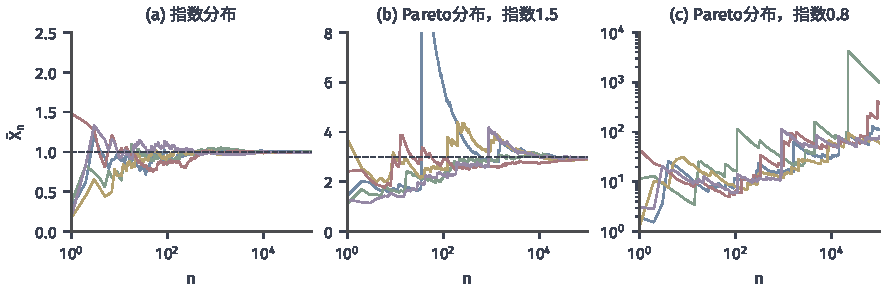
\includegraphics[width=150mm]{figures/02-abstract-mathematics/02-probability-spaces/matplotlib/conv-slln-paths/figure.pdf}
  \caption{独立同分布样本平均$\bar X_n$的路径，每个面板用固定随机种子画出$5$条，横轴为对数刻度，$n\leq10^5$。(a) 均值为$1$的指数分布，有有限方差；(b) 指数为$1.5$、下界为$1$的Pareto分布，均值为$3$（虚线），方差无穷；(c) 指数为$0.8$的Pareto分布，均值无穷，纵轴也为对数刻度。}
  \label{fig:conv-slln-paths}
\end{figure*}

\paragraph{函数的样本平均}
强大数律对任何满足矩条件的函数都成立。
设$g$可测且$\mathbb E|g(X_1)|<\infty$；$g(X_1),g(X_2),\ldots$仍独立同分布，把定理~\ref{thm:conv-slln}用于它们，得
\[
  \frac1n\sum_{k=1}^ng(X_k)\xrightarrow{\mathrm{a.s.}}\mathbb Eg(X_1).
\]
取$g=\mathbb I_B$，得到事件$\{X_k\in B\}$的经验频率几乎必然收敛到$P_{X_1}(B)$，这回答了章首的硬币问题。
取$g(x)=x^r$，$r$为正整数且$\mathbb E|X_1|^r<\infty$，得到样本$r$阶矩的收敛。
记$F$为$X_1$的分布函数，固定$x$并取$g=\mathbb I_{(-\infty,x]}$，经验分布函数在点$x$处几乎必然收敛到$F(x)$。

强大数律是渐近结论。
它不给出固定样本量下误差超过阈值的概率，也不给出收敛速度：图~\ref{fig:conv-slln-paths}(b)的样本平均同样收敛，但速度明显比(a)慢，这是定理本身看不出来的。
误差放大$\sqrt n$倍以后的分布规律由下一章（第~\ref{chap:weak-convergence-limit-theorems}章）的中心极限定理描述。
对一整族函数同时成立的收敛，例如经验分布函数在所有$x$上的一致收敛，属于\BookPartRef{part:inference-and-causal-identification}{卷四“推断与因果识别”部分}；观测相互依赖、平均沿时间进行的情形属于\BookPartRef{part:dynamical-systems-control-decision-and-games}{卷三“过程与轨迹演化”部分}。

\section{本章小结}
\label{sec:conv-summary}

\paragraph{三种收敛与两种失效}
章首问了随机误差以什么意义趋于零。
几乎处处收敛看每个样本结果的整条数列，依概率收敛看每个时刻坏事件的概率，$p$阶平均收敛看误差幅度的平均；几乎处处收敛和$p$阶平均收敛都蕴含依概率收敛，高阶平均收敛蕴含低阶平均收敛。
逆命题的失效有两种典型机制：二进区间扫描中坏事件越来越小却反复发生，所以依概率收敛和平均收敛都推不出几乎处处收敛；尖峰中坏事件只发生有限次却幅度极大，所以几乎处处收敛推不出平均收敛。
两种失效分别由两个工具修补。
Borel--Cantelli引理把“坏事件概率可求和”转化为“坏事件只发生有限次”，由此得到子列判据：依概率收敛恰好等价于每个子列都有几乎处处收敛的进一步子列。它使控制收敛这类逐点定理可以用于依概率收敛。
一致可积要求同一个阈值控制全族的尾部积分，它排除了稀有大值对平均误差的持续贡献；在依概率收敛下，它恰好等价于一阶平均收敛，期望的收敛随之而来，并可进一步传入固定信息下的条件期望。

\paragraph{强大数律的证明链}
章首还问了独立样本的平均何时沿几乎每条样本序列趋于总体均值。
Chebyshev界不可求和，说明单靠逐个时刻的二阶矩控制不够，需要控制整个过程的累计误差。
Kolmogorov最大不等式按第一次越过阈值的位置分解事件，使全程最大偏差与终点偏差共享同一个方差上界；由此，方差可和的独立级数几乎处处收敛；Kronecker引理再把加权级数的收敛化为平均值的收敛，得到方差可和条件下的强大数律。
只有一阶矩时，随项数增长的截断同时做到三件事：只改变有限多项，使截断项的方差满足可和条件，并保持期望的极限。
整条证明只用到有限事件分解、独立性、积分收敛定理和实数的完备性，不需要鞅或函数空间。

本章始终在同一个概率空间上比较$X_n$与$X$，误差$X_n-X$对每个样本结果都有意义。
下一章放弃这一前提，只比较分布：随机变量可以定义在不同的空间上，我们问它们的分布是否趋于某个极限分布，何时存在收敛的子列，以及如何识别并传递分布的极限。

\chapter{分布弱收敛、紧性与极限定理}
\label{chap:weak-convergence-limit-theorems}

第~\ref{chap:random-variable-convergence}章比较的随机变量都定义在同一个概率空间上，可以在每个样本点逐一比较取值。
统计中常见的极限却不是这样。设想我们研究率参数为$1$的指数分布：对样本量$n=5,20,100$分别重新抽取$20000$组数据，每组计算标准化均值$T_n=\sqrt n(\bar X_n-1)$。
不同$n$的数据分别生成，$T_5$与$T_{100}$之间没有可供逐点比较的共同样本点，我们能比较的只有它们的分布。
于是要问：“$T_n$的分布趋近$N(0,1)$”究竟指什么？得到这一结论后，能读出哪些概率和平均量的极限？事先不知道极限是什么时，分布列至少在什么条件下有收敛的子列？又用什么工具确认子列的极限恰好是正态分布？

这些问题按依赖关系排成本章的五节。
第~\ref{sec:wlim-weak-convergence}节在给定候选极限的前提下定义分布趋近：实轴上比较分布函数，一般度量空间上比较有界连续函数的积分，然后整理开闭集、边界与无界积分的判据。
第~\ref{sec:wlim-tightness}节去掉候选极限，用一致紧性保证弱收敛子列存在，这就是Prokhorov定理。
子列极限可能不止一个，因此第~\ref{sec:wlim-characteristic}节引入特征函数：它把分布写成一个确定的函数，把独立和变成乘积，并通过L\'evy连续性定理把函数的逐点收敛转回分布的弱收敛。
实际统计量往往由几个渐近量组合而成，第~\ref{sec:wlim-joint-transform}节说明联合分布怎样收敛、连续变换和随机标准化怎样传递极限。
第~\ref{sec:wlim-clt}节把这些工具合在一起，证明独立同分布、独立非同分布和随机向量三种情形的中心极限定理。

\section{概率分布列的弱收敛}
\label{sec:wlim-weak-convergence}

本节给定一列概率分布$P_n$和一个候选极限$P$，研究怎样判定$P_n$趋近$P$，以及这一结论允许我们读出哪些事件概率和积分的极限。
我们先在实轴上用分布函数表述，再改用连续测试函数推广到度量空间，最后比较不同收敛方式并整理事件与积分的判据。

\subsection{实轴上的分布收敛}

\paragraph{逐点比较分布函数的困难}
实值随机变量$X$的分布由分布函数$F(x)=\mathbb P(X\leq x)$完全确定，\BookChapterRef{chap:random-variables}{卷一“随机变量与概率分布”章}用它描述过离散与连续两类分布。
要说一列分布函数$F_n$趋近$F$，最直接的想法是要求每个阈值$x$处都有$F_n(x)\to F(x)$。
下面的例子说明这个要求过强。

\begin{example}[移动的点质量]
\label{ex:wlim-moving-point-mass}
令$P_n=\delta_{1/n}$是位于$1/n$的点质量，$P=\delta_0$是位于原点的点质量。它们的分布函数分别是
\[
  F_n(x)=\mathbb I_{[1/n,\infty)}(x),\qquad F(x)=\mathbb I_{[0,\infty)}(x).
\]
当$x<0$时两者都等于$0$；当$x>0$时，只要$n>1/x$就有$F_n(x)=1=F(x)$。
唯一的例外是$x=0$：对每个$n$都有$F_n(0)=0$，而$F(0)=1$。
\end{example}

图~\ref{fig:wlim-point-mass-cdf}画出了这一现象。
点质量的位置$1/n$在几何上越来越接近原点，分布函数的跳跃点也随之左移；但跳跃点始终在原点右侧，所以阈值恰好取在原点时，$F_n(0)$永远停在$0$。
失败只发生在极限分布函数$F$的跳跃点上，而那正是概率质量最终停留的位置。

\begin{figure}[htbp]
  \centering
  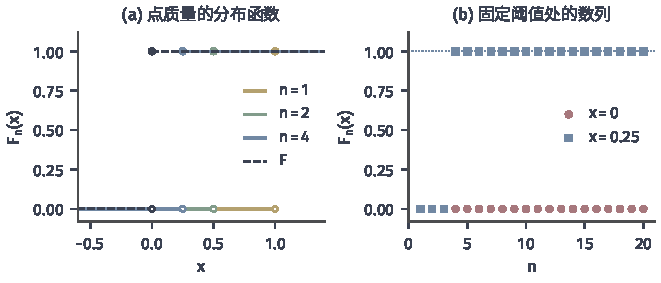
\includegraphics[width=112mm]{figures/02-abstract-mathematics/02-probability-spaces/matplotlib/wlim-point-mass-cdf/figure.pdf}
  \caption{点质量$\delta_{1/n}$的分布函数。(a) $n=1,2,4$时的$F_n$（实线）与极限$\delta_0$的分布函数$F$（虚线），实心点表示跳跃处取上方的值，空心点表示该处不取的值。(b) 固定阈值$x=0$与$x=0.25$时数列$F_n(x)$的取值，点线是$F(x)$。$x=0.25$处从$n=4$起$F_n(x)=1$；$x=0$处$F_n(0)$始终为$0$，而$F(0)=1$。}
  \label{fig:wlim-point-mass-cdf}
\end{figure}

\paragraph{连续点上的分布收敛}
例~\ref{ex:wlim-moving-point-mass}提示我们，只应在极限分布函数的连续点上要求收敛。

\begin{definition}[依分布收敛]
\label{def:wlim-convergence-in-distribution}
设$F_n$与$F$是实轴上的分布函数。若对$F$的每个连续点$x$都有$F_n(x)\to F(x)$，则称$F_n$\term{依分布收敛}（convergence in distribution）到$F$。
对分布函数分别为$F_n$和$F$的实值随机变量，同样称$X_n$依分布收敛到$X$，记作$X_n\Rightarrow X$。
\end{definition}

被排除的点不多。$F$单调不减，每个跳跃点$x$对应纵轴上的一个开区间$(F(x-),F(x))$，不同跳跃点的区间互不相交。
每个区间都含有理数，所以跳跃点至多可数，连续点在实轴上稠密。
极限因此是唯一的：若$F_n$同时依分布收敛到$F$和$G$，则$F$与$G$在两者公共连续点上相等，这些点仍然稠密；再由右连续性，从右侧逼近任一点即得$F=G$。

\paragraph{收敛的是分布而不是变量}
定义~\ref{def:wlim-convergence-in-distribution}只用到各个$X_n$的分布。
$X_n$可以定义在各自的概率空间$(\Omega_n,\mathcal F_n,\mathbb P_n)$上，$X$也可以换成任何与它同分布的随机变量，结论不受影响。
所以$X_n\Rightarrow X$实际是关于分布列$P_{X_n}$与分布$P_X$的陈述，它不要求这些变量共同实现，也不涉及$X_n$与$X$之间的差。
章首的模拟研究正是这种情形：每个$n$的数据单独生成，“$T_n$依分布趋近$N(0,1)$”有意义，“$T_n-Z$很小”却连定义都没有。

\subsection{度量空间上的弱收敛}

\paragraph{用有界连续函数检验}
分布函数依赖实数的大小顺序。随机向量、随机序列或随机函数的取值空间没有这样的顺序，我们需要一种不依赖顺序的比较方式。
自然的想法是挑选一类测试函数$h$，比较积分$\int h\,dP_n$与$\int h\,dP$。
事件的示性函数不适合做测试：例~\ref{ex:wlim-moving-point-mass}中$\delta_{1/n}(\{0\})=0$，而$\delta_0(\{0\})=1$，质量的微小移动就让它跳变。
连续函数则不会因微小移动而跳变。下面设$S$是度量空间，配以Borel $\sigma$代数，记$C_b(S)$为$S$上全体有界连续实值函数。

\begin{definition}[弱收敛]
\label{def:wlim-weak}
设$P_n$与$P$是度量空间$S$上的Borel概率测度。若对每个$h\in C_b(S)$都有
\[
  \int_S h\,dP_n\to\int_S h\,dP,
\]
则称$P_n$\term{弱收敛}（weak convergence）到$P$，记作$P_n\Rightarrow P$。
对取值于$S$的随机对象，若$P_{X_n}\Rightarrow P_X$，也称$X_n$依分布收敛到$X$，记作$X_n\Rightarrow X$。
\end{definition}

有界性保证每个测试积分有限；连续性保证取值的微小移动只引起测试值的微小变化。
由定理~\ref{thm:pmod-change-of-variables}，$\int h\,dP_{X_n}=\mathbb E\,h(X_n)$，所以随机对象的条件可以写成：对每个$h\in C_b(S)$，$\mathbb E\,h(X_n)\to\mathbb E\,h(X)$，其中各个期望分别在$X_n$与$X$所在的概率空间上计算。
回到移动的点质量，$\int h\,d\delta_{1/n}=h(1/n)\to h(0)$，所以$\delta_{1/n}\Rightarrow\delta_0$。
这里只使用一类测试函数，不需要在测度集合上另外构造范数或拓扑结构。

\paragraph{闭集的连续逼近与极限的唯一性}
连续测试函数虽然不能直接取成示性函数，却能从上方逼近闭集的示性函数。
这一构造既用来说明弱极限唯一，也是下文开闭集判据的出发点。

\begin{lemma}[闭集的距离逼近]
\label{lem:wlim-closed-approximation}
设$F$是度量空间$S$中的非空闭集，$d(x,F)=\inf_{y\in F}d(x,y)$。对正整数$k$令
\[
  h_k(x)=\max\{0,\,1-k\,d(x,F)\}.
\]
则每个$h_k$连续且$0\leq h_k\leq1$，在$F$上等于$1$；并且对每个$x\in S$，$h_k(x)$随$k$单调不增地趋于$\mathbb I_F(x)$。
\end{lemma}

\begin{proof}
由三角不等式，$|d(x,F)-d(y,F)|\leq d(x,y)$，所以$x\mapsto d(x,F)$连续，$h_k$连续且取值在$[0,1]$中。
若$x\in F$，则$d(x,F)=0$，$h_k(x)=1$。若$x\notin F$，因$F$闭，存在以$x$为中心的球与$F$不交，故$d(x,F)>0$；当$k>1/d(x,F)$时$h_k(x)=0$。$h_k$关于$k$单调不增是因为$1-k\,d(x,F)$关于$k$不增。
\end{proof}

\begin{lemma}[弱极限的唯一性]
\label{lem:wlim-uniqueness-limit}
设$P,Q$是度量空间$S$上的Borel概率测度。若对每个$h\in C_b(S)$都有$\int h\,dP=\int h\,dQ$，则$P=Q$。特别地，若$P_n\Rightarrow P$且$P_n\Rightarrow Q$，则$P=Q$。
\end{lemma}

\begin{proof}
对非空闭集$F$取引理~\ref{lem:wlim-closed-approximation}中的$h_k$。$h_k\to\mathbb I_F$逐点成立且$|h_k|\leq1$，由控制收敛定理，$P(F)=\lim_k\int h_k\,dP=\lim_k\int h_k\,dQ=Q(F)$；空集上两者都为零。
闭集族对有限交封闭，并且生成Borel $\sigma$代数，由定理~\ref{thm:measure-pi-lambda-uniqueness}得$P=Q$。
若$P_n$同时弱收敛到$P$和$Q$，则$\int h\,dP$与$\int h\,dQ$都是同一数列$\int h\,dP_n$的极限，从而相等。
\end{proof}

图~\ref{fig:wlim-closed-set-portmanteau}(a)以闭区间$F=[-1,0]$为例画出$h_k$：它们是一族梯形，平顶覆盖$F$，两侧斜坡宽度为$1/k$，随$k$增大而收窄，从上方压向$F$的示性函数。

\begin{figure}[htbp]
  \centering
  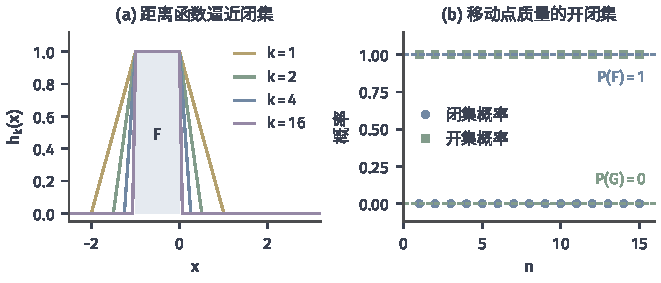
\includegraphics[width=112mm]{figures/02-abstract-mathematics/02-probability-spaces/matplotlib/wlim-closed-set-portmanteau/figure.pdf}
  \caption{闭集的连续逼近与开闭集上的概率界。(a) 闭集$F=[-1,0]$（浅蓝区域）的距离逼近$h_k(x)=\max\{0,1-k\,d(x,F)\}$，$k=1,2,4,16$。(b) 对$P_n=\delta_{1/n}$与$P=\delta_0$，圆点是闭集$F=(-\infty,0]$的概率$P_n(F)=0$，方点是开集$G=(0,\infty)$的概率$P_n(G)=1$，虚线分别是极限测度的概率$P(F)=1$与$P(G)=0$。}
  \label{fig:wlim-closed-set-portmanteau}
\end{figure}

\paragraph{与分布函数判据的等价}
在实轴上我们现在有两种定义：分布函数在连续点收敛，以及有界连续函数的积分收敛。
下面的定理说明二者一致，因此本章此后不再区分“依分布收敛”与“弱收敛”所指的分布趋近。

\begin{theorem}[实轴上两种定义的等价]
\label{thm:wlim-real-equivalence}
设$P_n,P$是$\mathbb R$上的Borel概率测度，分布函数分别为$F_n,F$。则$P_n\Rightarrow P$当且仅当$F$的每个连续点$x$处都有$F_n(x)\to F(x)$。
\end{theorem}

\begin{proof}
先证弱收敛推出分布函数收敛。固定$F$的连续点$x$和$\delta>0$，令$h_+$在$(-\infty,x]$上等于$1$、在$[x+\delta,\infty)$上等于$0$、中间线性下降；令$h_-$在$(-\infty,x-\delta]$上等于$1$、在$[x,\infty)$上等于$0$、中间线性下降。
两者都有界连续，并且$h_-\leq\mathbb I_{(-\infty,x]}\leq h_+$。对$P_n$积分得$\int h_-\,dP_n\leq F_n(x)\leq\int h_+\,dP_n$，令$n\to\infty$，
\[
  \begin{aligned}
  F(x-\delta)&\leq\int h_-\,dP\leq\liminf_nF_n(x)\\
  &\leq\limsup_nF_n(x)\leq\int h_+\,dP\leq F(x+\delta).
  \end{aligned}
\]
两端的不等式来自$\mathbb I_{(-\infty,x-\delta]}\leq h_-$与$h_+\leq\mathbb I_{(-\infty,x+\delta]}$。令$\delta\downarrow0$，由$F$在$x$处连续，两端都趋于$F(x)$。

再证反方向。设$h\in C_b(\mathbb R)$，$|h|\leq M$，固定$\varepsilon\in(0,1)$。
由于$F$的连续点稠密且$F(-\infty)=0$、$F(\infty)=1$，可取$F$的连续点$a<b$使$F(a)<\varepsilon$、$1-F(b)<\varepsilon$。
$h$在紧区间$[a,b]$上一致连续（定理~\ref{thm:metric-heine-cantor}），取$\eta>0$使$|x-y|\leq\eta$时$|h(x)-h(y)|<\varepsilon$；再取$F$的连续点$a=x_0<x_1<\dots<x_m=b$，相邻间距不超过$\eta$。
令$g=\sum_{j=1}^mh(x_j)\mathbb I_{(x_{j-1},x_j]}$，则在$(a,b]$上$|h-g|<\varepsilon$，在$(a,b]$外$g=0$。于是对$Q=P_n$或$Q=P$都有
\[
  \Bigl|\int h\,dQ-\int g\,dQ\Bigr|\leq\varepsilon+M\,Q\bigl(\mathbb R\setminus(a,b]\bigr).
\]
又$\int g\,dP_n=\sum_jh(x_j)\bigl(F_n(x_j)-F_n(x_{j-1})\bigr)\to\int g\,dP$，且$P_n(\mathbb R\setminus(a,b])=F_n(a)+1-F_n(b)\to F(a)+1-F(b)<2\varepsilon$。
合并得$\limsup_n|\int h\,dP_n-\int h\,dP|\leq2\varepsilon+4M\varepsilon$，而$\varepsilon$任意。
\end{proof}

图~\ref{fig:wlim-halfline-sandwich}展示了正向证明的两个动作：(a)中两条连续斜坡从两侧夹住半直线的示性函数；(b)以标准正态分布函数为例，上下界$F(x+\delta)$与$F(x-\delta)$随$\delta\to0$收拢到$F(x)$，这一步正是连续点条件发挥作用的地方。
反向证明把实轴分成紧区间和两端尾部分别处理，这样的分割不能省去：$h(x)=\sin(x^2)$有界连续，但在整条实轴上不一致连续，不能用一个统一的阶梯函数逼近；尾部只能依靠概率质量小来控制。

\begin{figure}[htbp]
  \centering
  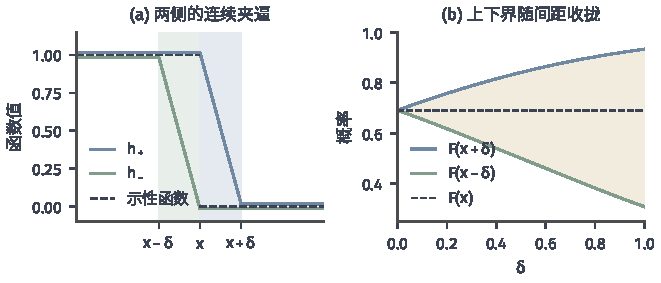
\includegraphics[width=112mm]{figures/02-abstract-mathematics/02-probability-spaces/matplotlib/wlim-halfline-sandwich/figure.pdf}
  \caption{用连续函数夹住半直线的示性函数。(a) 阈值$x=0$、间距$\delta=0.5$时的斜坡函数$h_-\leq\mathbb I_{(-\infty,x]}\leq h_+$，两条曲线略作上下错开以便区分。(b) 取$F$为标准正态分布函数、$x=0.5$，上界$F(x+\delta)$与下界$F(x-\delta)$随$\delta$减小收拢到$F(0.5)\approx0.691$（虚线）。}
  \label{fig:wlim-halfline-sandwich}
\end{figure}

\subsection{与依概率收敛的关系}

\paragraph{依概率收敛推出分布收敛}
当$X_n$与$X$定义在同一概率空间上时，第~\ref{chap:random-variable-convergence}章的依概率收敛（定义~\ref{def:conv-probability}）要求对每个$\varepsilon>0$都有$\mathbb P(\lVert X_n-X\rVert>\varepsilon)\to0$。
它比较的是逐样本误差，自然应当比只比较分布的弱收敛更强。证明用到该章的子列判据（定理~\ref{thm:conv-subsequence}）：$X_n\xrightarrow{\mathbb P}X$当且仅当每个子列都有进一步的子列几乎必然收敛到$X$。

\begin{theorem}[依概率收敛推出依分布收敛]
\label{thm:wlim-probability-implies-distribution}
设$\bm X_n,\bm X$是同一概率空间上的$\mathbb R^d$值随机向量。若$\bm X_n\xrightarrow{\mathbb P}\bm X$，则$\bm X_n\Rightarrow\bm X$。
\end{theorem}

\begin{proof}
设$h\in C_b(\mathbb R^d)$，$|h|\leq M$。若$\mathbb E\,h(\bm X_n)\not\to\mathbb E\,h(\bm X)$，则存在$\varepsilon>0$及子列$n_k$，使$|\mathbb E\,h(\bm X_{n_k})-\mathbb E\,h(\bm X)|\geq\varepsilon$对所有$k$成立。
由子列判据，$n_k$中还有子列$n_{k_j}$使$\bm X_{n_{k_j}}\to\bm X$几乎必然成立；$h$连续，故$h(\bm X_{n_{k_j}})\to h(\bm X)$几乎必然成立。
这些变量都以常数$M$为界，由控制收敛定理得$\mathbb E\,h(\bm X_{n_{k_j}})\to\mathbb E\,h(\bm X)$，与上面的不等式矛盾。
\end{proof}

同一论证适用于可分度量空间上的随机对象，这里不需要完备性。在可分的取值空间中$d(X_n,X)$是随机变量，依概率收敛定义为对每个$\varepsilon>0$都有$\mathbb P(d(X_n,X)>\varepsilon)\to0$；对实值变量$d(X_n,X)$使用子列判据，再重复上面的控制收敛论证，即得$X_n\Rightarrow X$。

\paragraph{向常数的分布收敛}
反方向一般不成立，但极限是常数时成立。此时依概率收敛只涉及$X_n$自身偏离常数$\bm c$的概率，不需要共同的极限变量。

\begin{theorem}[向常数的分布收敛]
\label{thm:wlim-constant-limit}
设$\bm X_n$是$\mathbb R^d$值随机向量（可以定义在不同概率空间上），$\bm c\in\mathbb R^d$为常向量。若$\bm X_n\Rightarrow\delta_{\bm c}$，则对每个$\varepsilon>0$都有$\mathbb P(\lVert\bm X_n-\bm c\rVert\geq\varepsilon)\to0$。
\end{theorem}

\begin{proof}
令$h(\bm x)=\min\{1,\lVert\bm x-\bm c\rVert/\varepsilon\}$，它有界连续，$h(\bm c)=0$，并且在$\{\lVert\bm x-\bm c\rVert\geq\varepsilon\}$上等于$1$。于是
\[
  \mathbb P(\lVert\bm X_n-\bm c\rVert\geq\varepsilon)\leq\mathbb E\,h(\bm X_n)\to h(\bm c)=0.
\]
不等式成立是因为$h$非负且在事件$\{\lVert\bm X_n-\bm c\rVert\geq\varepsilon\}$上等于$1$，极限来自依分布收敛的定义。
\end{proof}

当各个$\bm X_n$定义在不同概率空间上时，上式左端在各自的空间中计算，“$\bm X_n$依概率收敛到常数$\bm c$”仍然有意义，后文的Slutsky规则会用到这种形式。
与定理~\ref{thm:wlim-probability-implies-distribution}合起来，向常数的依分布收敛与依概率收敛等价。

\paragraph{同分布序列未必依概率收敛}
极限不是常数时，弱收敛不能推出依概率收敛。第~\ref{chap:probability-models}章的例~\ref{ex:pmod-alternating-bits}已经用交替序列说明，同分布的随机变量可以在样本点上相距很远；这里把它改写成符号形式，检验收敛方式的逆向关系。

\begin{example}[交替符号序列]
\label{ex:wlim-alternating-sign}
设$Z$以相等概率取$\pm1$，令$X_n=(-1)^nZ$。$-Z$与$Z$同分布，所以每个$X_n$都与$Z$同分布，$X_n\Rightarrow Z$平凡成立。
但当$n$为奇数时，$|X_n-Z|=2|Z|=2$恒成立，$\mathbb P(|X_n-Z|>1)=1$，所以$X_n$不依概率收敛到$Z$。
事实上$X_n$不依概率收敛到任何随机变量：偶数项恒等于$Z$，奇数项恒等于$-Z$，两个子列的极限不同。
\end{example}

弱收敛只记录各个$X_n$的分布，不记录$X_n$与$Z$在同一样本点上怎样配对；例~\ref{ex:wlim-alternating-sign}中分布始终不变，配对却在同号与反号之间交替。第~\ref{sec:wlim-joint-transform}节会看到，这种配对信息正是联合分布要补充的内容。

\subsection{开闭集与连续集上的概率}

\paragraph{开闭集上的概率界}
弱收敛用函数积分定义，但我们常常关心事件概率$P_n(A)$是否趋于$P(A)$。
移动的点质量说明不能对所有事件期望这一点：如图~\ref{fig:wlim-closed-set-portmanteau}(b)所示，对闭集$F=(-\infty,0]$有$P_n(F)=0<1=P(F)$，对开集$G=(0,\infty)$有$P_n(G)=1>0=P(G)$。
这里的质量原本在开集$G$内部，极限时落到$G$的边界点$0$上，而$0$属于闭集$F$。
质量落到边界上，可以让极限测度给闭集更多概率、给开集更少概率；反方向的跳变却不会发生。下面的定理把这一观察变成等价判据。

\begin{theorem}[\term{Portmanteau定理}]
\label{thm:wlim-portmanteau}
设$P_n,P$是度量空间$S$上的Borel概率测度。以下四条等价：
\begin{enumerate}
  \item $P_n\Rightarrow P$；
  \item 对每个闭集$F$，$\limsup_nP_n(F)\leq P(F)$；
  \item 对每个开集$G$，$\liminf_nP_n(G)\geq P(G)$；
  \item 对每个满足$P(\partial A)=0$的Borel集$A$，$P_n(A)\to P(A)$。
\end{enumerate}
\end{theorem}

\begin{proof}
由(1)推(2)。$F$为空集时结论平凡。对非空闭集$F$取引理~\ref{lem:wlim-closed-approximation}的$h_k$。由$\mathbb I_F\leq h_k$，
\[
  \limsup_nP_n(F)\leq\lim_n\int h_k\,dP_n=\int h_k\,dP.
\]
令$k\to\infty$，由控制收敛定理右端趋于$P(F)$。

(2)与(3)等价，因为开集的补集是闭集，而$P_n(G)=1-P_n(S\setminus G)$。

由(2)(3)推(4)。记$A^\circ$与$\overline A$为$A$的内部和闭包，$\partial A=\overline A\setminus A^\circ$。由$P(\partial A)=0$得$P(A^\circ)=P(A)=P(\overline A)$，于是
\[
  \begin{aligned}
  \limsup_nP_n(A)&\leq\limsup_nP_n(\overline A)\leq P(\overline A)=P(A),\\
  \liminf_nP_n(A)&\geq\liminf_nP_n(A^\circ)\geq P(A^\circ)=P(A).
  \end{aligned}
\]

由(4)推(1)。设$h\in C_b(S)$。对$h$作正仿射变换不改变结论，故不妨设$0<h<1$。由Tonelli定理（定理~\ref{thm:analysis-tonelli-fubini}），对任一概率测度$Q$，
\[
  \int h\,dQ=\int_S\int_0^1\mathbb I_{\{t<h(x)\}}\,dt\,Q(dx)=\int_0^1Q(h>t)\,dt.
\]
$h$连续，所以$\{h>t\}$是开集、$\{h\geq t\}$是闭集，边界含于$\{h=t\}$。集合$\{h=t\}$对不同$t$互不相交，其中$P$概率为正的至多可数个，因此除可数个$t$外都有$P(h=t)=0$，从而$P_n(h>t)\to P(h>t)$。
被积函数以$1$为界，对$dt$在$[0,1]$上使用控制收敛定理，即得$\int h\,dP_n\to\int h\,dP$。
\end{proof}

定理的(2)(3)是单向的：闭集的概率在极限处只可能增加，开集的概率只可能减少，因为质量可以从开集内部移到边界上，而边界属于相应的闭集。
证明的最后一步用水平集$\{h>t\}$把一个连续测试函数分解成一族开集，这是从事件概率回到积分的通用桥梁。

\paragraph{边界零质量的集合}
定理~\ref{thm:wlim-portmanteau}的(4)给出一类保证概率收敛的事件：满足$P(\partial A)=0$的Borel集合称为$P$的\term{连续集}（continuity set）。
在实轴上取$A=(-\infty,x]$，其边界是$\{x\}$，$P(\{x\})=F(x)-F(x-)$，所以$A$是连续集恰好等价于$x$是$F$的连续点。
定义~\ref{def:wlim-convergence-in-distribution}中“只在连续点要求收敛”的规定，因而是一般边界零质量条件在半直线上的特例。

边界零质量是充分条件而不是必要条件。若$P_n=P=\delta_0$对所有$n$成立，取$A=\{0\}$，则$P(\partial A)=1$，而$P_n(A)=P(A)$对所有$n$都成立。
条件说明的是：只要边界上没有极限质量，质量在边界两侧的移动就不影响概率的极限；边界上有质量时，需要另外检查质量从哪一侧趋近。

\subsection{分布积分的极限}

\paragraph{无界函数的积分}
弱收敛的定义已经保证有界连续函数的积分收敛。可是均值、方差等矩来自无界函数$x$、$x^2$，定义本身不覆盖它们。
第~\ref{chap:random-variable-convergence}章的尖峰变量（例~\ref{ex:conv-spike}）说明这里确有缺口：$U\sim\mathrm{Unif}[0,1)$，$X_n=n\mathbb I_{(0,1/n)}(U)$以概率$1/n$取$n$、其余时候取$0$。
那里关心$X_n$在样本点上趋于零而期望恒为$1$；这里只看它们的分布。

\begin{example}[尖峰分布]
\label{ex:wlim-spike-distribution}
令$P_n=(1-1/n)\delta_0+(1/n)\delta_n$，即上述$X_n$的分布。对$h\in C_b(\mathbb R)$，$|h|\leq M$，
\[
  \int h\,dP_n=\Bigl(1-\frac1n\Bigr)h(0)+\frac1nh(n)\to h(0),
\]
因为$|h(n)|/n\leq M/n\to0$。所以$P_n\Rightarrow\delta_0$。但对每个$n$都有$\int x\,P_n(dx)=1$，而极限的均值是$0$。
\end{example}

图~\ref{fig:wlim-spike-mean}(a)画出$n=10$与$n=40$的尖峰分布：远处的点质量越来越小，却越来越远，二者乘积保持为$1$。
(b)比较均值与截断均值$\int\min\{x,M\}\,dP_n=\min\{n,M\}/n$：截断函数$\min\{x,M\}$在分布的支撑$[0,\infty)$上有界连续，它的积分随$n$增大趋于零，符合弱收敛；不截断的均值则停在$1$。
差别完全来自尾部：远处很小的质量乘上很大的函数值，仍贡献了不消失的积分。

\begin{figure}[htbp]
  \centering
  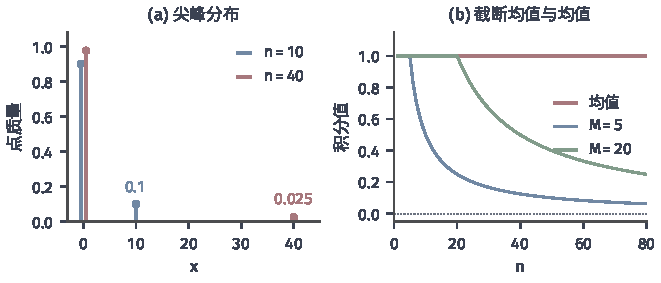
\includegraphics[width=112mm]{figures/02-abstract-mathematics/02-probability-spaces/matplotlib/wlim-spike-mean/figure.pdf}
  \caption{弱收敛但均值不收敛的尖峰分布$P_n=(1-1/n)\delta_0+(1/n)\delta_n$。(a) $n=10$与$n=40$时的点质量，原点处的两根竖线略作左右错开。(b) 均值$\int x\,dP_n=1$与截断均值$\int\min\{x,M\}\,dP_n=\min\{n,M\}/n$（$M=5,20$）随$n$的变化。}
  \label{fig:wlim-spike-mean}
\end{figure}

\paragraph{沿分布列的一致可积}
第~\ref{chap:random-variable-convergence}章用一致可积（定义~\ref{def:conv-uniform-integrability}）控制同一概率空间上随机变量的尾部积分。只看分布时，同样的尾部条件可以直接写在分布列上。

\begin{definition}[沿分布列的一致可积]
\label{def:wlim-ui-sequence}
设$P_n$是度量空间$S$上的Borel概率测度，$h:S\to\mathbb R$连续。若
\[
  \lim_{M\to\infty}\sup_n\int|h|\,\mathbb I_{\{|h|>M\}}\,dP_n=0,
\]
则称$h$关于$\{P_n\}$一致可积。
\end{definition}

若$X_n$的分布是$P_n$，这正是随机变量族$\{h(X_n)\}$的一致可积性；不同的是各个$X_n$可以定义在不同概率空间上。
尖峰分布不满足这一条件：取$h(x)=x$，当$n>M$时$\int|x|\,\mathbb I_{\{|x|>M\}}\,dP_n=1$。

\begin{theorem}[一致可积下的积分极限]
\label{thm:wlim-ui-integral}
设$P_n\Rightarrow P$，$h:S\to\mathbb R$连续且关于$\{P_n\}$一致可积。则$h$关于$P$可积，并且$\int h\,dP_n\to\int h\,dP$。
\end{theorem}

\begin{proof}
记$\tau(M)=\sup_n\int|h|\,\mathbb I_{\{|h|>M\}}\,dP_n$。

第一步，极限测度下的可积性。取$M_0$使$\tau(M_0)\leq1$，则
\[
  \sup_n\int|h|\,dP_n\leq M_0+1.
\]
对每个$L>0$，函数$\min\{|h|,L\}$有界连续，因此
\[
  \int\min\{|h|,L\}\,dP=\lim_n\int\min\{|h|,L\}\,dP_n\leq M_0+1.
\]
令$L\to\infty$，由单调收敛定理得$\int|h|\,dP\leq M_0+1$。于是$|h|\,\mathbb I_{\{|h|>M\}}\leq|h|$且逐点趋于零，由控制收敛定理，$\int|h|\,\mathbb I_{\{|h|>M\}}\,dP\to0$。

第二步，截断。令$h_M=\max\{-M,\min\{h,M\}\}$，它有界连续，并且$|h-h_M|\leq|h|\,\mathbb I_{\{|h|>M\}}$。于是
\[
  \Bigl|\int h\,dP_n-\int h\,dP\Bigr|\leq\tau(M)+\Bigl|\int h_M\,dP_n-\int h_M\,dP\Bigr|+\int|h|\,\mathbb I_{\{|h|>M\}}\,dP.
\]
先令$n\to\infty$，中间一项趋于零；再令$M\to\infty$，其余两项趋于零。
\end{proof}

证明的两次极限顺序不能交换：截断阈值$M$固定时，弱收敛处理有界部分；一致可积保证尾部误差对所有$n$同时小，才允许最后令$M\to\infty$。
尖峰分布在第二步失效：取$h(x)=x$时，对每个$M$都有$\tau(M)=1$，尾部误差不随$M$增大而减小。

\paragraph{均值与矩的收敛}
在$\mathbb R^d$上，最常用的无界函数是坐标$x_j$、乘积$x_ix_j$与范数的幂$\lVert\bm x\rVert^p$。下面给出一个易于检验的充分条件。

\begin{theorem}[矩的收敛]
\label{thm:wlim-moment-convergence}
设$\mathbb R^d$上的概率测度$P_n\Rightarrow P$，并且对某个$p>0$与$\delta>0$，
\[
  K=\sup_n\int\lVert\bm x\rVert^{p+\delta}\,P_n(d\bm x)<\infty.
\]
则对每个满足$|h(\bm x)|\leq C(1+\lVert\bm x\rVert^p)$的连续函数$h$，都有$\int h\,dP_n\to\int h\,dP$。
特别地，$p\geq1$时各坐标的均值收敛，$p\geq2$时二阶矩与协方差收敛。
\end{theorem}

\begin{proof}
令$r=(p+\delta)/p>1$。在$\{|h|>M\}$上$|h|=|h|^r|h|^{1-r}\leq|h|^rM^{1-r}$，并且由$(a+b)^r\leq2^{r-1}(a^r+b^r)$，
\[
  |h|^r\leq C^r2^{r-1}\bigl(1+\lVert\bm x\rVert^{p+\delta}\bigr).
\]
因此$\sup_n\int|h|\,\mathbb I_{\{|h|>M\}}\,dP_n\leq M^{1-r}C^r2^{r-1}(1+K)\to0$，再用定理~\ref{thm:wlim-ui-integral}。
坐标满足$|x_j|\leq\lVert\bm x\rVert\leq1+\lVert\bm x\rVert^p$（$p\geq1$），乘积满足$|x_ix_j|\leq\lVert\bm x\rVert^2\leq1+\lVert\bm x\rVert^p$（$p\geq2$），于是均值与二阶矩收敛，协方差由它们组合而成。
\end{proof}

这个条件要求略高于$p$阶的矩一致有界，仅有$p$阶矩一致有界还不够：尖峰分布的一阶矩恒为$1$，均值却不收敛到极限分布的均值；它的$1+\delta$阶矩等于$n^\delta$，确实没有一致上界。
把弱收敛与矩控制合成一种更强的分布距离，并用于比较分布和优化问题，是\BookPartRef{part:probability-distributions}{卷四“概率分布”部分}的任务。

\section{概率分布族的紧性}
\label{sec:wlim-tightness}

上一节总是先有候选极限$P$，再检验$P_n$是否趋近它。中心极限定理一类问题的困难恰在于极限需要被找出来。
本节先不指定极限，研究一族概率分布能否抽出弱收敛子列：先区分单个分布与整族分布的质量控制，再给出判别条件和子列存在定理，最后说明怎样从子列回到整列。

\subsection{紧性与一致紧性}

\paragraph{质量留在紧集中}
实数列有界时总有收敛子列，有界性阻止了数列跑向无穷远。
对概率分布列，相应的危险是概率质量跑出任何固定范围，例如$\delta_n$的全部质量随$n$移向无穷远，在极限中不留下任何东西。
第~\ref{chap:metric-spaces}章的紧集是度量空间中“既有界又不漏点”的范围，我们用它来约束质量的位置。

\begin{definition}[紧性与一致紧性]
\label{def:wlim-tight}
设$S$是度量空间。若对每个$\varepsilon>0$都存在紧集$K\subseteq S$使$P(K)>1-\varepsilon$，则称Borel概率测度$P$是紧的。
若对每个$\varepsilon>0$都存在\emph{同一个}紧集$K$，使族$\Pi$中每个$P$都满足$P(K)>1-\varepsilon$，则称概率族$\Pi$一致紧（uniformly tight），这一性质称为\term{一致紧性}。
\end{definition}

两者的差别在量词次序。紧性是“对每个$P$，存在$K$”，紧集可以随$P$改变；一致紧性是“存在$K$，对每个$P$”，紧集只能随精度$\varepsilon$改变，不能随族中成员改变。
一致紧性约束的是概率质量所在的范围，不约束质量在这个范围内怎样分布。

\paragraph{Polish空间上的单个分布}
在常用的取值空间中，单个概率测度总是紧的。所需的空间条件是：度量空间完备，并且有可数稠密子集，这样的空间称为\term{Polish空间}（Polish space）。$\mathbb R^d$、可数集配以离散度量，以及后续部分中的许多序列和函数空间都属于此类。

\begin{theorem}[Polish空间上的概率测度是紧的]
\label{thm:wlim-polish-tight}
设$S$是Polish空间，则$S$上每个Borel概率测度$P$都是紧的。
\end{theorem}

\begin{proof}
取$S$的可数稠密子集$\{s_1,s_2,\ldots\}$，固定$\varepsilon>0$。对每个正整数$m$，闭球$\overline B(s_j,1/m)$（$j\geq1$）覆盖$S$；由概率测度的下连续性，存在$N_m$使
\[
  P\Bigl(\bigcup_{j\leq N_m}\overline B(s_j,1/m)\Bigr)>1-\varepsilon2^{-m}.
\]
令$K=\bigcap_{m\geq1}\bigcup_{j\leq N_m}\overline B(s_j,1/m)$。$K$是闭集的交，因而闭；对每个$m$，$K$被有限个半径$1/m$的闭球覆盖，因而全有界。
完备空间的闭子集完备，由定理~\ref{thm:metric-complete-totally-bounded}，$K$紧。最后$P(S\setminus K)\leq\sum_m\varepsilon2^{-m}=\varepsilon$。
\end{proof}

证明用到三个结构：可分性提供可数个球心，概率的下连续性把无限覆盖截成有限覆盖，完备性保证有限覆盖的交确实是紧集。

\paragraph{逐个紧不推出一致紧}
定理~\ref{thm:wlim-polish-tight}只说明每个分布单独是紧的。点质量族$\{\delta_n:n\geq1\}$说明这不能推出一致紧：每个$\delta_n$的全部质量在单点$\{n\}$上，单点是紧集；但实轴上任何紧集$K$都有界，含于某个$[-R,R]$，当$n>R$时$\delta_n(K)=0$。

图~\ref{fig:wlim-escape-tight}(a)用“族内最大外部概率”$R\mapsto\sup_nP_n(|x|>R)$比较三族分布，一致紧性等价于这条曲线随$R\to\infty$趋于零。
$\{\delta_n\}$的曲线恒为$1$。尖峰分布族的曲线是$1/(\lfloor R\rfloor+1)$，趋于零，所以尖峰分布族一致紧，尽管它的均值不收敛到极限分布的均值；这说明一致紧性与上一节的一致可积控制的是不同的东西。
方差在$(1,2]$中的正态族由方差最大的成员控制，曲线是$\mathbb P(|N(0,2)|>R)$。图(b)把$\delta_n$的位置与一个固定窗口$[-R,R]$放在一起，窗口之外的点质量不断出现。

\begin{figure}[htbp]
  \centering
  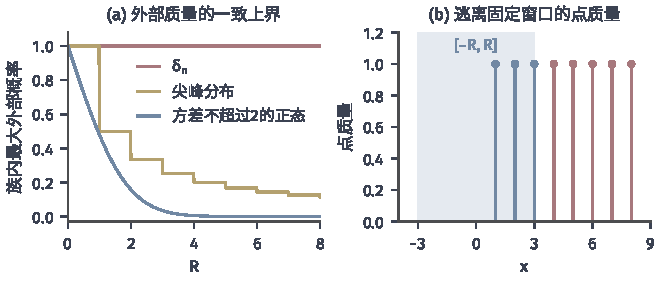
\includegraphics[width=112mm]{figures/02-abstract-mathematics/02-probability-spaces/matplotlib/wlim-escape-tight/figure.pdf}
  \caption{逃逸的点质量与一致紧的分布族。(a) 族内最大外部概率$\sup_nP_n(|x|>R)$：$\{\delta_n\}$恒为$1$；尖峰分布族$\{(1-1/n)\delta_0+(1/n)\delta_n\}$为$1/(\lfloor R\rfloor+1)$；正态族$\{N(0,1+1/n)\}$为$\mathbb P(|N(0,2)|>R)$。(b) 点质量$\delta_1,\ldots,\delta_8$与窗口$[-3,3]$（浅蓝区域），窗口外的点质量以红色标出。}
  \label{fig:wlim-escape-tight}
\end{figure}

\subsection{一致紧性的判别}

\paragraph{矩的一致上界}
在$\mathbb R^d$中，有界闭集紧（Heine--Borel判据），所以一致紧性就是大球外概率对全族一致消失：对每个$\varepsilon>0$存在$R$，使$\sup_nP_n(\lVert\bm x\rVert>R)<\varepsilon$。
Markov不等式（定理~\ref{thm:pmod-markov}）把这种尾部概率交给矩来控制。

\begin{theorem}[矩上界推出一致紧]
\label{thm:wlim-moment-tightness}
设$P_n$是$\mathbb R^d$上的概率测度。若对某个$p>0$有$C=\sup_n\int\lVert\bm x\rVert^p\,P_n(d\bm x)<\infty$，则$\{P_n\}$一致紧。
\end{theorem}

\begin{proof}
闭球$\overline B(\bm 0,R)$紧，并且由Markov不等式，$P_n(\lVert\bm x\rVert>R)\leq C/R^p$对所有$n$成立。取$R$使$C/R^p<\varepsilon$即可。
\end{proof}

定理要求的是矩的统一上界，逐项有限不够：$\delta_n$的每阶矩都有限，但$\int|x|^p\,d\delta_n=n^p$没有统一上界。
定理也只提供取得弱极限子列所需的质量控制，不说明整列收敛，更不说明同阶矩收敛：尖峰分布满足$\sup_n\int|x|\,dP_n=1$，因而一致紧，但均值不收敛到极限分布的均值。

另一个常用的一致紧来源是弱收敛本身。

\begin{lemma}[弱收敛列一致紧]
\label{lem:wlim-convergent-tight}
设$\mathbb R^d$上的概率测度$P_n\Rightarrow P$，则$\{P_n\}$一致紧。
\end{lemma}

\begin{proof}
固定$\varepsilon>0$，取$R$使$P(\lVert\bm x\rVert\geq R)<\varepsilon$。集合$\{\lVert\bm x\rVert\geq R\}$是闭集，由定理~\ref{thm:wlim-portmanteau}，$\limsup_nP_n(\lVert\bm x\rVert\geq R)\leq P(\lVert\bm x\rVert\geq R)<\varepsilon$，所以存在$N$使$n\geq N$时$P_n(\lVert\bm x\rVert\geq R)<\varepsilon$。
前$N-1$个测度各自是紧的：对单个概率测度$P_n$，$P_n(\lVert\bm x\rVert\geq r)\to0$（$r\to\infty$），所以各自存在使外部概率小于$\varepsilon$的半径。把$R$增大到这些半径的最大值，紧集$\overline B(\bm 0,R)$即对全族适用。
\end{proof}

\paragraph{紧次水平集}
定理~\ref{thm:wlim-moment-tightness}的证明实际只用到一点：函数$\lVert\bm x\rVert^p$不超过给定水平的点构成紧集。这一结构可以推广到一般度量空间。

\begin{theorem}[紧次水平集的控制函数]
\label{thm:wlim-sublevel-tightness}
设$S$是度量空间，$V:S\to[0,\infty)$可测，并且对每个$R\geq0$，次水平集$\{V\leq R\}$紧。若$C=\sup_n\int V\,dP_n<\infty$，则$\{P_n\}$一致紧。
\end{theorem}

\begin{proof}
由Markov不等式，$P_n(V>R)\leq C/R$对所有$n$成立，而$\{V\leq R\}$是紧集。取$R>C/\varepsilon$即可。
\end{proof}

推广时起作用的是“次水平集紧”；只找到一个积分一致有界的函数并不够，因为在一般度量空间中有界闭集未必紧。例如在自然数集$\mathbb N$上取离散度量（不同点距离为$1$），它是Polish空间。
令$V(x)=d(x,0)\leq1$，则$\sup_n\int V\,d\delta_n\leq1$；但$\{V\leq1\}=\mathbb N$不紧，离散空间的紧集只能是有限集，$\{\delta_n\}$也不一致紧。

\subsection{弱收敛子列的存在}

\paragraph{有理点上的对角线选择}
现在在实轴上构造弱收敛子列。分布函数取值在$[0,1]$中，每个固定阈值处的数列都有收敛子列；困难在于阈值有不可数多个。
我们只在可数个有理点上取子列，再用单调性把极限延拓到整条实轴。

\begin{lemma}[\term{Helly选择定理}]
\label{lem:wlim-helly}
设$F_n$是实轴上的分布函数列。则存在子列$F_{n_k}$及单调不减、右连续、取值于$[0,1]$的函数$G$，使在$G$的每个连续点$x$处都有$F_{n_k}(x)\to G(x)$。
\end{lemma}

\begin{proof}
把有理数排成$q_1,q_2,\ldots$。数列$F_n(q_1)$在$[0,1]$中有界，有收敛子列；在这个子列中，$F_n(q_2)$又有收敛的子子列；如此依次取下去，得到一串嵌套的子列。取第$k$个子列中的第$k$项为$n_k$，则对每个$j$，$(n_k)_{k\geq j}$都是第$j$个子列的子列，于是$F_{n_k}(q)$对每个有理数$q$都收敛，记极限为$H(q)$。

$H$在有理数上单调不减。令$G(x)=\inf\{H(q):q\in\mathbb Q,\,q>x\}$，它单调不减。
若$x_m\downarrow x$，对每个有理数$q>x$，当$m$充分大时$x_m<q$，故$\lim_mG(x_m)\leq H(q)$；对$q$取下确界得$\lim_mG(x_m)\leq G(x)$，而单调性给出反向不等式，所以$G$右连续。

设$x$是$G$的连续点。对有理数$s>x$，$F_{n_k}(x)\leq F_{n_k}(s)\to H(s)$，对$s$取下确界得$\limsup_kF_{n_k}(x)\leq G(x)$。
对$y<x$取有理数$q\in(y,x)$，则$G(y)\leq H(q)$，而$H(q)=\lim_kF_{n_k}(q)\leq\liminf_kF_{n_k}(x)$；令$y\uparrow x$，由连续性得$G(x)\leq\liminf_kF_{n_k}(x)$。
\end{proof}

对角线步骤只保证每个有理点处的局部极限存在；它不保证$G(-\infty)=0$、$G(\infty)=1$。
图~\ref{fig:wlim-helly-selection}(b)给出了缺口：$P_n=\tfrac12N(0,1)+\tfrac12\delta_n$的分布函数逐点收敛到$G=\tfrac12\Phi$，一半质量随$\delta_n$逃到无穷远，$G(\infty)=1/2$，$G$不是概率分布的分布函数。

\paragraph{一致紧性保证总质量为一}
补上缺口需要两件事：一致紧性阻止质量逃逸；一个单调右连续、两端极限为$0$和$1$的函数确实是某个概率分布的分布函数。后一件事可以用分位变换直接构造。

\begin{lemma}[由分布函数构造分布]
\label{lem:wlim-quantile-construction}
设$G:\mathbb R\to[0,1]$单调不减、右连续，且$G(-\infty)=0$、$G(\infty)=1$。在$(0,1)$上取Lebesgue测度为概率，令$G^{-}(u)=\inf\{x:G(x)\geq u\}$。则$G^{-}$的分布函数是$G$；并且具有同一分布函数的两个Borel概率测度相等。
\end{lemma}

\begin{proof}
对$u\in(0,1)$，两端极限保证集合$\{x:G(x)\geq u\}$非空且有下界，$G^{-}(u)$有限；由右连续性，下确界可以取到，即$G(G^{-}(u))\geq u$。
于是$G^{-}(u)\leq x$当且仅当$u\leq G(x)$：若$u\leq G(x)$，则$x$属于上述集合，$G^{-}(u)\leq x$；反之$G(x)\geq G(G^{-}(u))\geq u$。
所以$\{u:G^{-}(u)\leq x\}=(0,G(x)]\cap(0,1)$，其Lebesgue测度为$G(x)$。
唯一性：半直线$(-\infty,x]$构成对有限交封闭的集合族，生成Borel $\sigma$代数，由定理~\ref{thm:measure-pi-lambda-uniqueness}即得。
\end{proof}

\begin{theorem}[实轴上的弱收敛子列]
\label{thm:wlim-real-subsequence}
设$\{P_n\}$是$\mathbb R$上一致紧的概率测度列，则存在子列$P_{n_k}$及概率测度$P$使$P_{n_k}\Rightarrow P$。
\end{theorem}

\begin{proof}
对分布函数$F_n$应用引理~\ref{lem:wlim-helly}，得到子列$F_{n_k}$与函数$G$。固定$\varepsilon>0$，由一致紧性取$R$使$P_n([-R,R])>1-\varepsilon$对所有$n$成立。
取$G$的连续点$a<-R$与$b>R$，则$F_{n_k}(a)\leq P_{n_k}((-\infty,-R))<\varepsilon$，$F_{n_k}(b)\geq P_{n_k}([-R,R])>1-\varepsilon$，令$k\to\infty$得$G(a)\leq\varepsilon$、$G(b)\geq1-\varepsilon$。
$G$单调且$\varepsilon$任意，所以$G(-\infty)=0$、$G(\infty)=1$。由引理~\ref{lem:wlim-quantile-construction}，$G$是某个概率测度$P$的分布函数；再由定理~\ref{thm:wlim-real-equivalence}，$P_{n_k}\Rightarrow P$。
\end{proof}

对角线选择提供局部极限，一致紧性保证总质量仍为一，两步各司其职，不能互相替代。
图~\ref{fig:wlim-helly-selection}(a)展示选择本身：$P_n=N(\sin n,1)$的均值$\sin n$在$[-1,1]$中来回游走，整列不收敛；挑出均值越来越接近$0.5$的项$n=1,7,32,78$，它们的分布函数（彩色）逐渐贴近极限$\Phi(x-0.5)$（虚线）。这个族的方差都等于$1$，二阶矩一致有界，一致紧性由定理~\ref{thm:wlim-moment-tightness}保证。

\begin{figure*}[htbp]
  \centering
  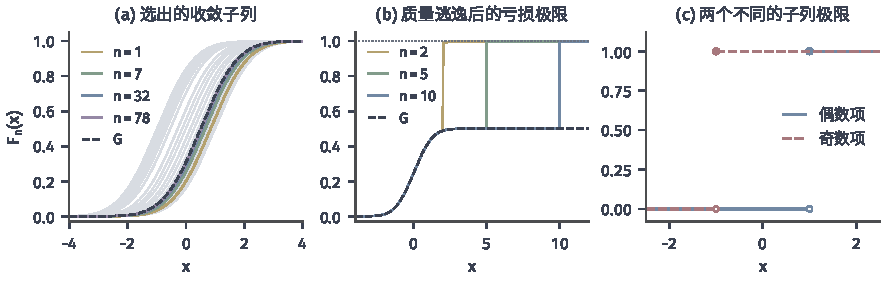
\includegraphics[width=150mm]{figures/02-abstract-mathematics/02-probability-spaces/matplotlib/wlim-helly-selection/figure.pdf}
  \caption{分布函数的子列选择。(a) $P_n=N(\sin n,1)$，灰线为$n=1,\ldots,30$的分布函数，彩色为均值依次接近$0.5$的项（$n=1,7,32,78$，均值约为$0.84,0.66,0.55,0.51$），虚线为极限$\Phi(x-0.5)$。(b) $P_n=\tfrac12N(0,1)+\tfrac12\delta_n$的分布函数（$n=2,5,10$）逐点趋于$G=\tfrac12\Phi$（虚线），$G(\infty)=1/2$。(c) $P_n=\delta_{(-1)^n}$，偶数项与奇数项的分布函数分别等于$\delta_1$与$\delta_{-1}$的分布函数。}
  \label{fig:wlim-helly-selection}
\end{figure*}

\paragraph{Prokhorov定理}
实轴上的构造推广到Polish空间，结论是子列存在与一致紧性等价。

\begin{theorem}[\term{Prokhorov定理}]
\label{thm:wlim-prokhorov}
设$S$是Polish空间，$\Pi$是$S$上的Borel概率测度族。则$\Pi$一致紧，当且仅当$\Pi$中每个序列都有弱收敛到某个Borel概率测度的子列。所得的极限不必属于$\Pi$。
\end{theorem}

一致紧推出子列存在的方向，实轴情形就是定理~\ref{thm:wlim-real-subsequence}；$\mathbb R^d$上可以用多元分布函数在有理点处作同样的对角线选择。
一般Polish空间的证明保留同一思路：先取一列紧集$K_m$使$\sup_{P\in\Pi}P(S\setminus K_m)<1/m$；在每个$K_m$中取可数稠密集，以其中的点为心、有理数为半径的闭球作有限并，得到一个可数集合族；对这个可数族作对角线选择，使子列在每个集合上的概率都收敛；再由这些极限值构造外测度，验证它限制在Borel集上是测度，并对每个开集满足Portmanteau定理中的下极限不等式。一致紧性保证构造出的测度总质量为一。完整论证可参考Kallenberg的概率论教材\scite{math-kallenberg2021probability}。

反方向的证明较短，我们完整写出。设$\Pi$中每个序列都有弱收敛子列，取$S$的可数稠密子集$\{s_j\}$，记开集$G_{m,N}=\bigcup_{j\leq N}B(s_j,1/m)$，固定$\varepsilon>0$。
我们断言：对每个$m$，存在$N_m$使$P(G_{m,N_m})>1-\varepsilon2^{-m}$对所有$P\in\Pi$成立。
否则存在$m$，对每个$N$都能取$P_N\in\Pi$使$P_N(G_{m,N})\leq1-\varepsilon2^{-m}$。按假设取子列$P_{N_k}\Rightarrow Q$。对固定的$N$，当$N_k\geq N$时$G_{m,N}\subseteq G_{m,N_k}$，由定理~\ref{thm:wlim-portmanteau}的开集判据，
\[
  Q(G_{m,N})\leq\liminf_kP_{N_k}(G_{m,N})\leq\liminf_kP_{N_k}(G_{m,N_k})\leq1-\varepsilon2^{-m}.
\]
但$G_{m,N}$随$N$增大到整个$S$，令$N\to\infty$得$Q(S)<1$，矛盾。
于是令$K=\bigcap_m\overline{G_{m,N_m}}$。与定理~\ref{thm:wlim-polish-tight}的证明一样，$K$闭且全有界，在完备空间中紧，并且$P(S\setminus K)\leq\sum_m\varepsilon2^{-m}=\varepsilon$对所有$P\in\Pi$成立。

\paragraph{从子列到整列}
Prokhorov定理只给出子列。要证明整列收敛，还需要下面的子列原理。

\begin{lemma}[子列原理]
\label{lem:wlim-subsequence-principle}
设$P_n,P$是度量空间上的Borel概率测度。若$\{P_n\}$的每个子列都有进一步的子列弱收敛到同一个$P$，则$P_n\Rightarrow P$。
\end{lemma}

\begin{proof}
若不然，存在$h\in C_b(S)$、$\varepsilon>0$与子列$n_k$，使$|\int h\,dP_{n_k}-\int h\,dP|\geq\varepsilon$对所有$k$成立。这个子列的任何进一步子列都不能弱收敛到$P$，与假设矛盾。
\end{proof}

由此得到证明整列弱收敛的标准路线：先证明一致紧，由Prokhorov定理知道每个子列都有弱收敛的进一步子列；再证明所有可能的子列极限都等于同一个$P$；最后由子列原理得到$P_n\Rightarrow P$。
第二步不能省略。图~\ref{fig:wlim-helly-selection}(c)中的$P_n=\delta_{(-1)^n}$全部集中在紧集$[-1,1]$上，一致紧；偶数项弱收敛到$\delta_1$，奇数项弱收敛到$\delta_{-1}$，两个子列极限不同，整列不收敛。
识别子列极限需要一种能够唯一确定分布、又便于取极限的工具，下一节的特征函数承担这个任务。

\section{概率分布的积分变换}
\label{sec:wlim-characteristic}

上一节留下的问题是识别子列极限。直接比较分布并不方便：独立随机变量之和的分布要用二重积分计算，逐个识别子列极限更无从下手。
本节把每个概率分布$P$变成一个确定的函数$\varphi_P$，这一函数把独立和变成乘积，唯一确定分布，并且其逐点收敛在适当条件下等价于弱收敛。
需要区分两种变换：这里的$P\mapsto\varphi_P$输出一个复值函数；下一节的推前$P\mapsto g_\#P$输出另一个概率分布。
所需工具只有复指数、第~\ref{chap:measure-spaces}章的积分与积分极限，以及上一节的紧性与弱子列，不预设一般Fourier分析或复分析。

\subsection{特征函数的定义与运算}

\paragraph{复值函数的积分}
对实数$\theta$，复指数$e^{i\theta}=\cos\theta+i\sin\theta$满足$|e^{i\theta}|=1$、$e^{i(\theta+\eta)}=e^{i\theta}e^{i\eta}$，其共轭是$e^{-i\theta}$。
对复值可测函数$f=u+iv$，若$|f|$可积（等价地，$u$与$v$都可积），定义$\int f\,d\mu=\int u\,d\mu+i\int v\,d\mu$。这一积分对复系数线性，控制收敛定理可以分别用于实部与虚部。
我们还需要不等式$|\int f\,d\mu|\leq\int|f|\,d\mu$：若$\int f\,d\mu=re^{i\alpha}$，$r\geq0$，则
\[
  r=e^{-i\alpha}\int f\,d\mu=\int\operatorname{Re}\bigl(e^{-i\alpha}f\bigr)\,d\mu\leq\int|f|\,d\mu,
\]
中间一步用到$r$是实数，所以虚部的积分为零。
最后，若$X\perp Y$，$f,g$是有界复值可测函数，把$f(X)g(Y)$的实部与虚部展开成四个实值乘积，分别应用定理~\ref{thm:pmod-product-expectation}，得到$\mathbb E[f(X)g(Y)]=\mathbb E f(X)\,\mathbb E g(Y)$。

\paragraph{特征函数的定义}
复指数$x\mapsto e^{itx}$有界连续，它对任何概率分布都可积。

\begin{definition}[特征函数]
\label{def:wlim-characteristic}
设$P$是$\mathbb R$上的Borel概率测度，称
\[
  \varphi_P(t)=\int_{\mathbb R}e^{itx}\,P(dx),\qquad t\in\mathbb R,
\]
为$P$的\term{特征函数}（characteristic function）。若实值随机变量$X$的分布为$P$，记$\varphi_X(t)=\mathbb E\,e^{itX}=\varphi_P(t)$。
对$\mathbb R^d$上的概率测度和$\mathbb R^d$值随机向量$\bm X$，相应地定义$\varphi_{\bm X}(\bm t)=\mathbb E\,e^{i\langle\bm t,\bm X\rangle}$，$\bm t\in\mathbb R^d$。
\end{definition}

特征函数只依赖分布，同分布的随机变量有相同的特征函数。下面的基本性质对任何分布成立，不要求均值或方差有限。

\begin{theorem}[特征函数的基本性质]
\label{thm:wlim-chf-basic}
设$\varphi$是$\mathbb R^d$上某个概率测度的特征函数，则$\varphi(\bm 0)=1$，$|\varphi(\bm t)|\leq1$，$\varphi(-\bm t)=\overline{\varphi(\bm t)}$，并且$\varphi$在$\mathbb R^d$上一致连续。
\end{theorem}

\begin{proof}
前三条分别来自$e^{0}=1$、$|\int f\,dP|\leq\int|f|\,dP$与$e^{-i\theta}=\overline{e^{i\theta}}$。对一致连续性，
\[
  |\varphi(\bm t+\bm s)-\varphi(\bm t)|=\Bigl|\mathbb E\bigl[e^{i\langle\bm t,\bm X\rangle}(e^{i\langle\bm s,\bm X\rangle}-1)\bigr]\Bigr|\leq\mathbb E\bigl|e^{i\langle\bm s,\bm X\rangle}-1\bigr|.
\]
右端与$\bm t$无关。当$\bm s\to\bm 0$时被积函数逐点趋于零且以$2$为界，由控制收敛定理趋于零。
\end{proof}

由第三条性质，若$X$与$-X$同分布，则$\varphi_X(t)=\varphi_{-X}(t)=\varphi_X(-t)=\overline{\varphi_X(t)}$，特征函数是实值的，这时它等于$\mathbb E\cos(tX)$。

\paragraph{仿射变换与独立和}
特征函数的用处首先在于运算规则简单。

\begin{theorem}[仿射变换与独立和]
\label{thm:wlim-chf-operations}
设$\bm X$是$\mathbb R^d$值随机向量。
\begin{enumerate}
  \item 对$m\times d$矩阵$\bm A$与$\bm b\in\mathbb R^m$，$\varphi_{\bm A\bm X+\bm b}(\bm t)=e^{i\langle\bm t,\bm b\rangle}\varphi_{\bm X}(\bm A^\top\bm t)$；特别地，实值情形$\varphi_{aX+b}(t)=e^{itb}\varphi_X(at)$。
  \item 若$\bm X\perp\bm Y$且二者都取值于$\mathbb R^d$，则$\varphi_{\bm X+\bm Y}=\varphi_{\bm X}\varphi_{\bm Y}$。
\end{enumerate}
\end{theorem}

\begin{proof}
第一条由$\langle\bm t,\bm A\bm X+\bm b\rangle=\langle\bm A^\top\bm t,\bm X\rangle+\langle\bm t,\bm b\rangle$及$e^{i(\theta+\eta)}=e^{i\theta}e^{i\eta}$得到。
第二条中$e^{i\langle\bm t,\bm X+\bm Y\rangle}=e^{i\langle\bm t,\bm X\rangle}e^{i\langle\bm t,\bm Y\rangle}$，两个因子分别是$\bm X$与$\bm Y$的有界复值函数，由独立性下的乘积公式即得。
\end{proof}

独立和的分布本身是一个二重积分。由定理~\ref{thm:pmod-independence-product}，$(\bm X,\bm Y)$的联合分布是乘积测度$P_{\bm X}\otimes P_{\bm Y}$，用Fubini定理得
\[
  \mathbb P(\bm X+\bm Y\in B)=\int P_{\bm Y}(B-\bm x)\,P_{\bm X}(d\bm x),\qquad B-\bm x=\{\bm y-\bm x:\bm y\in B\}.
\]
这个分布称为$P_{\bm X}$与$P_{\bm Y}$的\term{卷积}（convolution），记作$P_{\bm X}*P_{\bm Y}$。逐次计算$n$重卷积很繁琐，而定理~\ref{thm:wlim-chf-operations}说明它的特征函数只是各因子的乘积，中心极限定理的证明正是利用这一点。

乘积规则依赖独立性，不相关不够。设$X$在$\{-1,0,1\}$上均匀分布，$Y=\mathbb I_{\{X=0\}}$。由于$XY=0$恒成立且$\mathbb E X=0$，$\operatorname{Cov}(X,Y)=0$。
但$X+Y$以概率$1/3$取$-1$、以概率$2/3$取$1$，在$t=\pi$处$\varphi_{X+Y}(\pi)=-1$；而$\varphi_X(\pi)=(1+2\cos\pi)/3=-1/3$，$\varphi_Y(\pi)=2/3+e^{i\pi}/3=1/3$，乘积为$-1/9$。

\paragraph{几个常见分布的特征函数}
下面的计算将在后文反复使用。
若$X\sim\operatorname{Bernoulli}(p)$，则$\varphi_X(t)=1-p+pe^{it}$；二项分布$\operatorname{Bin}(n,p)$是$n$个独立Bernoulli变量之和，特征函数为$(1-p+pe^{it})^n$。
Rademacher变量$R$以相等概率取$\pm1$，$\varphi_R(t)=\cos t$。$\mathrm{Unif}[-1,1]$的特征函数是$\frac12\int_{-1}^1e^{itx}\,dx=\sin t/t$（$t\ne0$），在$t=0$处取$1$。

标准正态分布的特征函数需要稍作推导。记$\phi(x)=e^{-x^2/2}/\sqrt{2\pi}$。分布对称，故$\varphi(t)=\int\cos(tx)\phi(x)\,dx$。
由$|\cos a-\cos b|\leq|a-b|$，差商$[\cos((t+s)x)-\cos(tx)]/s$以$|x|$为界，而$|x|\phi(x)$可积，由控制收敛定理可以在积分号下求导；再用$\phi'(x)=-x\phi(x)$分部积分，
\[
  \varphi'(t)=-\int x\sin(tx)\phi(x)\,dx=\int\sin(tx)\phi'(x)\,dx=-t\varphi(t),
\]
边界项$\sin(tx)\phi(x)$在$\pm\infty$处为零。于是$(\varphi(t)e^{t^2/2})'=0$，结合$\varphi(0)=1$得
\begin{equation}
  \varphi_{N(0,1)}(t)=e^{-t^2/2}.
  \label{eq:wlim-normal-chf}
\end{equation}
由仿射规则，$N(\mu,\sigma^2)$的特征函数是$e^{i\mu t-\sigma^2t^2/2}$。两个独立正态变量$N(\mu_1,\sigma_1^2)$与$N(\mu_2,\sigma_2^2)$之和的特征函数是$e^{i(\mu_1+\mu_2)t-(\sigma_1^2+\sigma_2^2)t^2/2}$，正是$N(\mu_1+\mu_2,\sigma_1^2+\sigma_2^2)$的特征函数；待下一小节证明唯一性后，这就推出独立正态之和仍是正态。

多元正态分布也可以由此确定。设$\bm\Sigma$是$d\times d$半正定矩阵，取矩阵$\bm A$使$\bm A\bm A^\top=\bm\Sigma$，$\bm Z$的$d$个坐标独立且服从$N(0,1)$。称$\bm\mu+\bm A\bm Z$的分布为$N(\bm\mu,\bm\Sigma)$。由仿射规则和坐标独立，
\begin{equation}
  \varphi_{N(\bm\mu,\bm\Sigma)}(\bm t)=e^{i\langle\bm t,\bm\mu\rangle}\prod_{j=1}^de^{-(\bm A^\top\bm t)_j^2/2}=\exp\Bigl(i\langle\bm t,\bm\mu\rangle-\tfrac12\bm t^\top\bm\Sigma\bm t\Bigr).
  \label{eq:wlim-mvn-chf}
\end{equation}
右端只依赖$\bm\mu$与$\bm\Sigma$，唯一性定理证明后即知$N(\bm\mu,\bm\Sigma)$不依赖$\bm A$的选取。$\bm\Sigma$奇异时$\bm A$不满秩，分布集中在一个低维仿射子空间上，没有密度，但特征函数公式照样成立。

图~\ref{fig:wlim-characteristic-functions}(a)比较三个对称分布的特征函数：它们都是实值偶函数，在原点取$1$。Rademacher分布的$\cos t$周期性地回到$\pm1$，这对应于取值只在整数格点上的离散分布；均匀分布的$\sin t/t$在远处振荡衰减；正态分布的$e^{-t^2/2}$衰减最快。
(b)中Bernoulli$(0.3)$分布不对称，特征函数有非零虚部；它的模$|0.7+0.3e^{it}|$在$0.4$与$1$之间周期变化。

\begin{figure}[htbp]
  \centering
  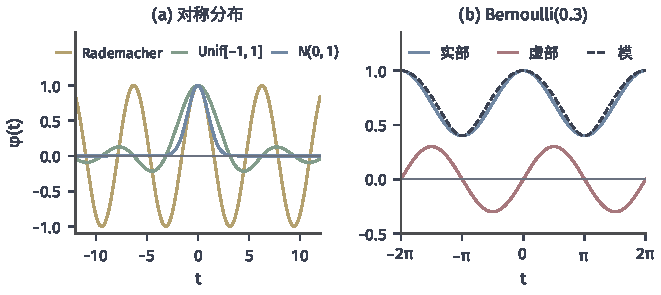
\includegraphics[width=112mm]{figures/02-abstract-mathematics/02-probability-spaces/matplotlib/wlim-characteristic-functions/figure.pdf}
  \caption{几个分布的特征函数。(a) Rademacher分布$\cos t$、$\mathrm{Unif}[-1,1]$分布$\sin t/t$与标准正态分布$e^{-t^2/2}$，三者都是实值偶函数。(b) $\operatorname{Bernoulli}(0.3)$分布的特征函数$0.7+0.3e^{it}$的实部、虚部与模，周期为$2\pi$，模的最小值为$0.4$。}
  \label{fig:wlim-characteristic-functions}
\end{figure}

\subsection{特征函数与矩}

\paragraph{矩条件下的求导}
特征函数在原点附近的行为记录了分布的矩。我们先说明有限绝对矩怎样给出可微性。证明反复使用不等式$|e^{iu}-1|=|\int_0^uie^{is}\,ds|\leq|u|$，$u\in\mathbb R$。

\begin{theorem}[有限矩与导数]
\label{thm:wlim-chf-derivatives}
设$X$是实值随机变量，$m$为正整数，$\mathbb E|X|^m<\infty$。则$\varphi_X$在$\mathbb R$上$m$阶连续可导，并且对$1\leq k\leq m$，
\[
  \varphi_X^{(k)}(t)=\mathbb E\bigl[(iX)^ke^{itX}\bigr],\qquad\text{特别地}\quad\mathbb E X^k=i^{-k}\varphi_X^{(k)}(0).
\]
\end{theorem}

\begin{proof}
由定理~\ref{thm:pmod-moment-monotone}，$\mathbb E|X|^k<\infty$对$k\leq m$成立。对$k$归纳，设$\varphi_X^{(k-1)}(t)=\mathbb E[(iX)^{k-1}e^{itX}]$（$k=1$时即定义）。对$s\neq0$，
\[
  \frac{\varphi_X^{(k-1)}(t+s)-\varphi_X^{(k-1)}(t)}{s}=\mathbb E\Bigl[(iX)^{k-1}e^{itX}\,\frac{e^{isX}-1}{s}\Bigr].
\]
期望内的量当$s\to0$时逐点趋于$(iX)^ke^{itX}$，模不超过$|X|^{k-1}\cdot|X|=|X|^k$，后者可积。沿任一趋于零的数列$s_j$用控制收敛定理，即得导数公式。
导数$\mathbb E[(iX)^ke^{itX}]$关于$t$连续，同样由控制收敛定理（控制函数$|X|^k$）得到。
\end{proof}

定理只建立了“有限绝对矩推出可微”这一方向。反过来由导数存在推出矩有限需要另外的论证，对奇数阶一般不成立，本章不使用。

\paragraph{二阶展开}
中心极限定理只需要特征函数在原点的二阶展开，而且只需要有限二阶矩。关键是复指数Taylor余项的一个双重估计。

\begin{lemma}[复指数的二阶余项]
\label{lem:wlim-exp-remainder}
对实数$u$，
\[
  \Bigl|e^{iu}-1-iu+\frac{u^2}2\Bigr|\leq\min\Bigl\{\frac{|u|^3}6,\,u^2\Bigr\}.
\]
\end{lemma}

\begin{proof}
设$u\geq0$（$u<0$时取共轭）。由$e^{is}-1=i\int_0^se^{ir}\,dr$并交换积分次序，
\[
  e^{iu}-1-iu=i\int_0^u(e^{is}-1)\,ds=-\int_0^u\!\!\int_0^se^{ir}\,dr\,ds=-\int_0^u(u-r)e^{ir}\,dr.
\]
又$\int_0^u(u-r)\,dr=u^2/2$，所以$e^{iu}-1-iu+u^2/2=-\int_0^u(u-r)(e^{ir}-1)\,dr$。
用$|e^{ir}-1|\leq r$得到上界$\int_0^u(u-r)r\,dr=u^3/6$；用$|e^{ir}-1|\leq2$得到上界$u^2$。
\end{proof}

\begin{theorem}[有限二阶矩下的展开]
\label{thm:wlim-chf-second-order}
设$\mathbb E X^2<\infty$，则当$t\to0$时
\[
  \varphi_X(t)=1+it\,\mathbb E X-\frac{t^2}2\,\mathbb E X^2+o(t^2).
\]
特别地，若$\mathbb E X=0$、$\operatorname{Var}X=\sigma^2$，则$\varphi_X(t)=1-\sigma^2t^2/2+o(t^2)$。
设$\bm X$是均值为$\bm\mu$、协方差矩阵为$\bm\Sigma$的$\mathbb R^d$值随机向量，则对固定方向$\bm a\in\mathbb R^d$，当$u\to0$时
\[
  \varphi_{\bm X-\bm\mu}(u\bm a)=1-\frac{u^2}2\,\bm a^\top\bm\Sigma\bm a+o(u^2).
\]
\end{theorem}

\begin{proof}
记$R(u)=e^{iu}-1-iu+u^2/2$，则$\varphi_X(t)-(1+it\,\mathbb E X-\tfrac12t^2\,\mathbb E X^2)=\mathbb E\,R(tX)$。由引理~\ref{lem:wlim-exp-remainder}，
\[
  \frac{|R(tX)|}{t^2}\leq\min\Bigl\{\frac{|t|\,|X|^3}6,\,X^2\Bigr\}.
\]
右端当$t\to0$时逐点趋于零，并以可积的$X^2$为界，由控制收敛定理$\mathbb E|R(tX)|/t^2\to0$。
向量情形把一维结论用于$Y=\bm a^\top(\bm X-\bm\mu)$：$\mathbb E Y=0$，$\operatorname{Var}Y=\bm a^\top\bm\Sigma\bm a$，并且$\varphi_{\bm X-\bm\mu}(u\bm a)=\varphi_Y(u)$。
\end{proof}

证明中的二阶控制$X^2$来自余项估计的第二部分，三阶估计只用于说明逐点趋于零，因此不需要三阶矩。结论也不要求矩母函数存在。

\subsection{反演与分布唯一性}

\paragraph{截断反演积分}
特征函数能否唯一确定分布？在实轴上，我们直接由特征函数恢复区间概率。先准备一个正弦积分的极限。

\begin{lemma}[正弦积分]
\label{lem:wlim-sine-integral}
令$S(y)=\int_0^y\frac{\sin u}u\,du$，$y\in\mathbb R$。则$S$是连续的奇函数，在$\mathbb R$上有界，并且$S(y)\to\pi/2$（$y\to\infty$）。
\end{lemma}

\begin{proof}
被积函数在$u=0$处按连续延拓取$1$，所以$S$连续；被积函数是偶函数，故$S$是奇函数。
对$y>0$，用$1/u=\int_0^\infty e^{-us}\,ds$（$u>0$）写成二重积分。由于$\int_0^y\int_0^\infty|\sin u|e^{-us}\,ds\,du=\int_0^y|\sin u|/u\,du\leq y$，Fubini定理允许交换次序：
\[
  S(y)=\int_0^\infty\!\!\int_0^y\sin u\,e^{-us}\,du\,ds=\int_0^\infty\frac{1-e^{-ys}(s\sin y+\cos y)}{1+s^2}\,ds,
\]
内层积分对$y$求导即可验证。右端第一部分积分为$\pi/2$；第二部分的模不超过$\int_0^\infty e^{-ys}\frac{s+1}{1+s^2}\,ds\leq\frac2y$，因为$(s+1)/(1+s^2)\leq2$。所以$|S(y)-\pi/2|\leq2/y\to0$。
$S$在每个有界区间上连续因而有界，在$[2,\infty)$上又被$\pi/2+1$控制；由奇性，$S$在整条实轴上有界。
\end{proof}

\begin{theorem}[反演公式]
\label{thm:wlim-inversion}
设$P$是$\mathbb R$上的概率测度，$a<b$。则
\[
  \lim_{T\to\infty}\frac1{2\pi}\int_{-T}^T\frac{e^{-ita}-e^{-itb}}{it}\,\varphi_P(t)\,dt=P\bigl((a,b)\bigr)+\frac12P(\{a\})+\frac12P(\{b\}),
\]
其中被积函数在$t=0$处按连续延拓取值$b-a$。特别地，若$a,b$都不是$P$的原子，极限就是$P((a,b))$。
\end{theorem}

\begin{proof}
记左端截断积分为$I_T$。由$\bigl|\frac{e^{-ita}-e^{-itb}}{it}\bigr|=\bigl|\int_a^be^{-itu}\,du\bigr|\leq b-a$，被积函数在$[-T,T]\times\mathbb R$上有界，对有限测度$dt\otimes P$用Fubini定理交换积分：
\[
  I_T=\int_{\mathbb R}J_T(x)\,P(dx),\qquad J_T(x)=\frac1{2\pi}\int_{-T}^T\frac{e^{it(x-a)}-e^{it(x-b)}}{it}\,dt.
\]
把$e^{itc}/(it)$拆成$\cos(tc)/(it)+\sin(tc)/t$。余弦部分的差$[\cos(t(x-a))-\cos(t(x-b))]/(it)$是$t$的奇函数，在对称区间上积分为零；正弦部分是偶函数。代换$u=tc$得$\int_0^T\sin(tc)/t\,dt=S(Tc)$，于是
\[
  J_T(x)=\frac1\pi\Bigl[S\bigl(T(x-a)\bigr)-S\bigl(T(x-b)\bigr)\Bigr].
\]
由引理~\ref{lem:wlim-sine-integral}，当$T\to\infty$时$S(Tc)\to\frac\pi2\operatorname{sgn}c$，所以$J_T(x)$在$x<a$或$x>b$时趋于$0$，在$a<x<b$时趋于$1$，在$x=a$或$x=b$时趋于$1/2$。
$J_T$以$2\sup|S|/\pi$为界，对有限测度$P$用控制收敛定理，即得结论。
\end{proof}

图~\ref{fig:wlim-inversion-atom}(a)画出区间$(0,1)$对应的截断核$J_T$：$T$增大时它逼近区间的示性函数，但在两个端点处稳定地取$1/2$。
(b)以$\operatorname{Bernoulli}(0.3)$为例，原子在$0$（质量$0.7$）与$1$（质量$0.3$）。区间$(-0.5,0.5)$的端点不是原子，$I_T\to0.7=P((-0.5,0.5))$；区间$(0,1)$的两个端点都是原子，$I_T\to\frac12\cdot0.7+\frac12\cdot0.3=0.5$，既不是$P((0,1))=0$也不是$P([0,1])=1$；区间$(0,2)$只有左端点是原子，极限为$0.35+0.3=0.65$。
所以反演公式不要求分布有密度，但含原子的端点只能恢复半个质量。

\begin{figure}[htbp]
  \centering
  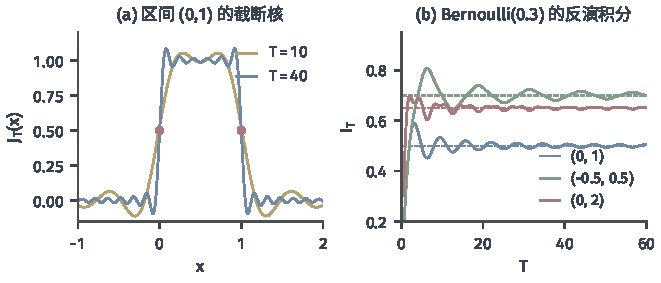
\includegraphics[width=112mm]{figures/02-abstract-mathematics/02-probability-spaces/matplotlib/wlim-inversion-atom/figure.pdf}
  \caption{截断反演积分在原子端点处给出半个质量。(a) 区间$(a,b)=(0,1)$的截断核$J_T(x)=[S(T(x-a))-S(T(x-b))]/\pi$，$T=10,40$，红点标出端点处的值$1/2$。(b) $P=\operatorname{Bernoulli}(0.3)$时三个区间的截断积分$I_T$随$T$的变化，虚线为反演公式给出的极限$0.5$、$0.7$与$0.65$。}
  \label{fig:wlim-inversion-atom}
\end{figure}

\paragraph{实轴上的唯一性}
反演公式立即说明，实轴上特征函数相同的两个分布相同。
设$\varphi_P=\varphi_Q$。两者原子合起来至多可数，对不是任一原子的$a<b$，反演公式给出$P((a,b))=Q((a,b))$。
令$a$沿非原子点趋于$-\infty$，得$P((-\infty,b))=Q((-\infty,b))$，对所有非原子点$b$成立；非原子点在实轴上稠密，从右侧逼近任一点$x$，由下连续性得$F_P(x)=F_Q(x)$，再由引理~\ref{lem:wlim-quantile-construction}中的唯一性部分得$P=Q$。

\paragraph{有限维的高斯平滑}
在$\mathbb R^d$上也可以写出多维区间的反演公式，但边界上的原子处理起来很繁琐。我们改用另一条路：给分布加上一点独立的高斯噪声，使它有一个由特征函数显式表示的密度，再让噪声消失。

\begin{lemma}[高斯平滑后的密度]
\label{lem:wlim-gaussian-smoothing}
设$\bm X$的分布为$P$，$\bm Z\sim N(\bm 0,\bm I_d)$与$\bm X$独立，$\varepsilon>0$。则$\bm X+\varepsilon\bm Z$有密度
\[
  g_\varepsilon(\bm y)=\frac1{(2\pi)^d}\int_{\mathbb R^d}e^{-i\langle\bm t,\bm y\rangle}e^{-\varepsilon^2\lVert\bm t\rVert^2/2}\varphi_P(\bm t)\,d\bm t.
\]
\end{lemma}

\begin{proof}
记$\phi_d$为$N(\bm 0,\bm I_d)$的密度。对Borel集$B$，由独立性、换元$\bm y=\bm x+\varepsilon\bm z$与Tonelli定理，
\[
  \begin{aligned}
  \mathbb P(\bm X+\varepsilon\bm Z\in B)&=\int\!\!\int\mathbb I_B(\bm x+\varepsilon\bm z)\phi_d(\bm z)\,d\bm z\,P(d\bm x)\\
  &=\int_B\int\varepsilon^{-d}\phi_d\Bigl(\frac{\bm y-\bm x}\varepsilon\Bigr)P(d\bm x)\,d\bm y.
  \end{aligned}
\]
把式~\eqref{eq:wlim-normal-chf}写成$\int e^{isw}\phi(w)\,dw=e^{-s^2/2}=\sqrt{2\pi}\,\phi(s)$，代换$w=\varepsilon\tau$、$s=v/\varepsilon$得$\varepsilon^{-1}\phi(v/\varepsilon)=\frac1{2\pi}\int e^{iv\tau}e^{-\varepsilon^2\tau^2/2}\,d\tau$；对$d$个坐标相乘，
\[
  \varepsilon^{-d}\phi_d\Bigl(\frac{\bm v}\varepsilon\Bigr)=\frac1{(2\pi)^d}\int e^{-i\langle\bm t,\bm v\rangle}e^{-\varepsilon^2\lVert\bm t\rVert^2/2}\,d\bm t,
\]
其中把$\bm t$换成$-\bm t$不改变积分。代入$\bm v=\bm y-\bm x$，被积函数的模不超过可积的$e^{-\varepsilon^2\lVert\bm t\rVert^2/2}$，用Fubini定理先对$P(d\bm x)$积分，$\int e^{i\langle\bm t,\bm x\rangle}P(d\bm x)=\varphi_P(\bm t)$，即得所述密度。
\end{proof}

\begin{theorem}[特征函数的唯一性]
\label{thm:wlim-uniqueness}
设$P,Q$是$\mathbb R^d$上的Borel概率测度。若$\varphi_P(\bm t)=\varphi_Q(\bm t)$对所有$\bm t\in\mathbb R^d$成立，则$P=Q$。
\end{theorem}

\begin{proof}
取$\bm X\sim P$、$\bm Y\sim Q$，各自配上独立的$\bm Z\sim N(\bm 0,\bm I_d)$。由引理~\ref{lem:wlim-gaussian-smoothing}，$\bm X+\varepsilon\bm Z$与$\bm Y+\varepsilon\bm Z$的密度由同一公式给出，二者同分布。
对$h\in C_b(\mathbb R^d)$，于是$\mathbb E\,h(\bm X+\varepsilon\bm Z)=\mathbb E\,h(\bm Y+\varepsilon\bm Z)$。令$\varepsilon\downarrow0$，被积量逐点收敛且有界，由控制收敛定理得$\int h\,dP=\int h\,dQ$；再由引理~\ref{lem:wlim-uniqueness-limit}，$P=Q$。
\end{proof}

这条证明对$d=1$同样适用，它没有用到下一节的Cramér--Wold判据，也没有预设一般的Fourier反演定理。高斯平滑把“特征函数相同”变成“平滑后的密度相同”，有界连续测试再把平滑撤去。

\subsection{特征函数与弱收敛}

\paragraph{弱收敛推出逐点收敛}
若$P_n\Rightarrow P$，对固定的$\bm t$，$\cos\langle\bm t,\bm x\rangle$与$\sin\langle\bm t,\bm x\rangle$都是有界连续函数，所以$\varphi_{P_n}(\bm t)\to\varphi_P(\bm t)$。
我们真正需要的是反方向：只知道特征函数逐点收敛，能否断定分布弱收敛，甚至在事先没有候选极限的情况下找到极限？

\paragraph{L\'evy连续性定理}
答案是肯定的，只需在原点处加一个连续性条件。

\begin{theorem}[\term{L\'evy连续性定理}]
\label{thm:wlim-levy}
设$P_n$是$\mathbb R^d$上的概率测度。
\begin{enumerate}
  \item 若$P_n\Rightarrow P$，则$\varphi_{P_n}(\bm t)\to\varphi_P(\bm t)$对每个$\bm t$成立。
  \item 若对每个$\bm t$，$\varphi_{P_n}(\bm t)$收敛到某个数$\varphi(\bm t)$，并且函数$\varphi$在$\bm 0$处连续，则存在概率测度$P$使$\varphi=\varphi_P$，并且$P_n\Rightarrow P$。
\end{enumerate}
\end{theorem}

第二条不要求预先给出候选极限，极限$P$由定理本身产生。原点连续性不能删去。

\begin{example}[方差趋于无穷的正态分布]
\label{ex:wlim-spreading-normal}
令$P_n=N(0,n)$，则$\varphi_{P_n}(t)=e^{-nt^2/2}$，其逐点极限$\varphi(t)$在$t=0$处为$1$、其余点为$0$，在原点不连续。
相应地，分布函数$F_n(x)=\Phi(x/\sqrt n)\to1/2$对每个$x$成立，极限不是任何分布函数：质量同时向两侧无穷远逃逸，$\{P_n\}$不一致紧，也没有弱收敛到概率测度的子列。
\end{example}

图~\ref{fig:wlim-levy-counterexample}对照了两面：(a)中特征函数越来越窄，只在原点保留高度$1$；(b)中分布函数越来越平，压向高度$1/2$的水平线。
特征函数在原点附近的急剧下降，正是分布在远处有大量质量的信号；下面的引理把这一对应写成不等式。

\begin{figure}[htbp]
  \centering
  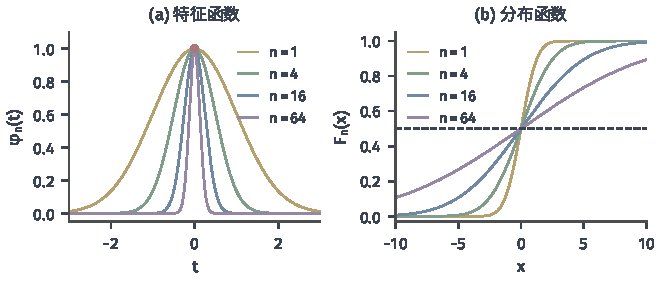
\includegraphics[width=112mm]{figures/02-abstract-mathematics/02-probability-spaces/matplotlib/wlim-levy-counterexample/figure.pdf}
  \caption{$P_n=N(0,n)$的特征函数与分布函数，$n=1,4,16,64$。(a) $\varphi_n(t)=e^{-nt^2/2}$的逐点极限在原点为$1$（红点）、其余点为$0$。(b) $F_n(x)=\Phi(x/\sqrt n)$逐点趋于$1/2$（虚线），不存在概率分布极限。}
  \label{fig:wlim-levy-counterexample}
\end{figure}

\paragraph{原点附近的积分控制}
\begin{lemma}[尾部概率的特征函数界]
\label{lem:wlim-tail-bound}
设$P$是$\mathbb R$上的概率测度，$u>0$。则
\[
  P\Bigl(\bigl\{x:|x|>\tfrac2u\bigr\}\Bigr)\leq\frac1u\int_{-u}^u\bigl(1-\varphi_P(t)\bigr)\,dt.
\]
\end{lemma}

\begin{proof}
对$x\neq0$，$\frac1u\int_{-u}^u(1-e^{itx})\,dt=2-\frac{2\sin(ux)}{ux}$，对$x=0$该积分为$0$。被积函数有界，用Fubini定理交换积分次序，
\[
  \frac1u\int_{-u}^u\bigl(1-\varphi_P(t)\bigr)\,dt=\int_{\mathbb R}\Bigl(2-\frac{2\sin(ux)}{ux}\Bigr)P(dx).
\]
由$|\sin y|\leq|y|$，右端被积函数非负；当$|ux|\geq2$时$|\sin(ux)/(ux)|\leq1/2$，被积函数至少为$1$。所以右端不小于$P(|x|\geq2/u)$。
\end{proof}

左端只用到$\varphi_P$在区间$[-u,u]$上的值：$u$越小，看到的是越远处的尾部。

\paragraph{连续性定理的证明}
定理~\ref{thm:wlim-levy}的第一条前面已经证明。第二条按“原点附近的积分控制、一致紧性、弱收敛子列、极限唯一”四步完成。

\begin{proof}[定理~\ref{thm:wlim-levy}第二条的证明]
先设$d=1$。由$\varphi_{P_n}(0)=1$得$\varphi(0)=1$。固定$\varepsilon>0$，由$\varphi$在原点连续，取$u>0$使$|1-\varphi(t)|<\varepsilon/2$对$|t|\leq u$成立，于是$\frac1u\int_{-u}^u|1-\varphi(t)|\,dt\leq\varepsilon$。
在$[-u,u]$上$|1-\varphi_{P_n}|\leq2$且逐点趋于$1-\varphi$，由控制收敛定理，
\[
  \frac1u\int_{-u}^u\bigl(1-\varphi_{P_n}(t)\bigr)\,dt\to\frac1u\int_{-u}^u\bigl(1-\varphi(t)\bigr)\,dt,
\]
后者的模不超过$\varepsilon$。所以存在$N$，当$n\geq N$时左端小于$2\varepsilon$，由引理~\ref{lem:wlim-tail-bound}得$P_n(|x|>2/u)<2\varepsilon$。前$N-1$个测度各自是紧的，把半径增大即可覆盖，于是$\{P_n\}$一致紧。

对一般$d$，第$j$个坐标在$P_n$下的特征函数是$s\mapsto\varphi_{P_n}(s\bm e_j)$，它逐点收敛到在$s=0$处连续的$\varphi(s\bm e_j)$。由一维情形，每个坐标的分布族一致紧；再由
\[
  P_n\bigl(\lVert\bm x\rVert_\infty>R\bigr)\leq\sum_{j=1}^dP_n(|x_j|>R),
\]
联合分布族一致紧。

由Prokhorov定理（定理~\ref{thm:wlim-prokhorov}），每个子列都有进一步的子列$P_{n_k}\Rightarrow Q$，$Q$是某个概率测度。由第一条，$\varphi_{P_{n_k}}\to\varphi_Q$逐点成立；而$\varphi_{P_{n_k}}\to\varphi$，所以$\varphi_Q=\varphi$。
任何两个子列极限都有特征函数$\varphi$，由定理~\ref{thm:wlim-uniqueness}它们是同一个测度$P$，且$\varphi=\varphi_P$。最后由子列原理（引理~\ref{lem:wlim-subsequence-principle}）得$P_n\Rightarrow P$。
\end{proof}

证明中坐标方向只负责一致紧性：坐标的尾部概率之和控制联合分布的尾部。识别联合极限时用的仍是全部$\bm t\in\mathbb R^d$上的特征函数，不能只由各坐标的边缘收敛代替。

\subsection{矩母函数及其适用条件（补充）}

\paragraph{有限域与各阶矩}
初等概率中常用矩母函数计算矩、识别分布。它和特征函数的区别在于指数是实的，因而可能发散。
对实值随机变量$X$，令$M_X(t)=\mathbb E\,e^{tX}\in(0,\infty]$，称为\term{矩母函数}（moment generating function），其有限域为$D_X=\{t:M_X(t)<\infty\}$。
$0\in D_X$总成立，但这远不足以读取矩；需要的条件是$M_X$在零点的某个开邻域$(-t_0,t_0)$内有限。

在此条件下取$0<a<t_0$，由$e^{a|X|}\leq e^{aX}+e^{-aX}$得$\mathbb E\,e^{a|X|}<\infty$，各阶矩都有限。
对$|t|\leq a'<a$，$|X|^ke^{tX}\leq|X|^ke^{a'|X|}\leq C_ke^{a|X|}$，其中$C_k=\sup_{y\geq0}y^ke^{-(a-a')y}<\infty$。这个可积控制允许像定理~\ref{thm:wlim-chf-derivatives}那样逐阶把求导移入期望，得到$M_X^{(k)}(t)=\mathbb E[X^ke^{tX}]$，特别是$M_X^{(k)}(0)=\mathbb E X^k$。

\paragraph{矩母函数与分布唯一性}
若$M_X=M_Y$在$(-t_0,t_0)$内有限，则$X$与$Y$同分布。下面的论证只用实参数幂级数与积分交换。

先说明特征函数在每一点都有半径统一的Taylor展开。对实数$s$与$|h|<t_0$，由$|e^{iv}-\sum_{k<n}(iv)^k/k!|\leq|v|^n/n!$（与引理~\ref{lem:wlim-exp-remainder}同样由积分余项得到），
\[
  \Bigl|\varphi_X(s+h)-\sum_{k<n}\frac{(ih)^k}{k!}\mathbb E\bigl[X^ke^{isX}\bigr]\Bigr|\leq\frac{|h|^n\,\mathbb E|X|^n}{n!}.
\]
由$\sum_n|h|^n\mathbb E|X|^n/n!=\mathbb E\,e^{|h||X|}<\infty$，右端趋于零，由定理~\ref{thm:wlim-chf-derivatives}，$i^k\mathbb E[X^ke^{isX}]=\varphi_X^{(k)}(s)$，所以$\varphi_X(s+h)=\sum_kh^k\varphi_X^{(k)}(s)/k!$对$|h|<t_0$成立，半径$t_0$与$s$无关，因为$|e^{isX}|=1$。

在$s=0$处，展开系数是各阶矩，由前一段它们由$M_X$在零点的导数确定，所以$\varphi_X=\varphi_Y$在$(-t_0,t_0)$上成立。
若两个特征函数在某点$s$的邻域内相等，则它们在$s$处的各阶导数相等，展开式在$(s-t_0,s+t_0)$上相同。从$s=\pm t_0/2$出发，相等区间扩大到$(-3t_0/2,3t_0/2)$；如此每次延伸$t_0/2$，覆盖整条实轴。最后由定理~\ref{thm:wlim-uniqueness}得$X$与$Y$同分布。

\paragraph{各阶矩有限不能代替矩母函数有限}
条件“在零点邻域内有限”不能换成“各阶矩都有限”。
令$Z\sim N(0,1)$、$X=e^Z$。由配方，$e^{kz}\phi(z)=e^{k^2/2}\phi(z-k)$，所以$\mathbb E\,e^{kZ}=e^{k^2/2}$，$X$的各阶矩$\mathbb E X^k=e^{k^2/2}$都有限；但对$t>0$，$te^z-z^2/2\to\infty$（$z\to\infty$），所以$M_X(t)=\infty$，$D_X=(-\infty,0]$。
这时上面基于指数可积的唯一性论证无法启动。事实上，密度$f(x)\bigl(1+\sin(2\pi\log x)\bigr)$（$f$为$X$的密度）与$X$有完全相同的各阶矩：$\int x^kf(x)\sin(2\pi\log x)\,dx=\mathbb E[e^{kZ}\sin(2\pi Z)]=e^{k^2/2}\,\mathbb E\sin(2\pi(Z+k))=0$，其中第二步再次使用上述配方，最后一步用到$k$是整数及$Z$的对称性。各阶矩一般不能唯一确定分布，本章不展开这一问题。
后面的中心极限定理只用定理~\ref{thm:wlim-chf-second-order}的二阶展开，不需要矩母函数。

\section{联合分布与函数变换的极限}
\label{sec:wlim-joint-transform}

统计量很少是单个渐近量本身。学生化均值是一个分子除以一个分母，回归系数的估计是几个样本矩的组合。
本节研究几个随机量组成的联合分布怎样收敛，以及对它们作函数变换后极限怎样传递：先补足边缘分布不包含的配对信息，再建立连续变换、随机标准化和近似替换的规则。
这些规则都不以中心极限定理为前提，下一节证明中心极限定理后可以直接使用。

\subsection{联合分布的收敛判据}

\paragraph{边缘相同、配对不同}
设对每个$n$，$X_n$与$Y_n$定义在同一个概率空间上，组成随机向量$(X_n,Y_n)$。
联合分布记录两组取值怎样配对，边缘分布只分别记录各自的规律。第~\ref{chap:probability-models}章的例~\ref{ex:pmod-bernoulli-couplings}已经说明相同的边缘可以有不同的配对；这里关心的是这种差别对极限的影响。

\begin{example}[交替配对]
\label{ex:wlim-alternating-pairing}
设$Z$以相等概率取$\pm1$。$(Z,Z)$与$(Z,-Z)$的两个边缘都是$\pm1$上的均匀分布，但前者的坐标和是$2Z$，后者的坐标和恒为$0$。
令$n$为偶数时$(X_n,Y_n)=(Z,Z)$，$n$为奇数时$(X_n,Y_n)=(Z,-Z)$。两个边缘分布对所有$n$都不变，当然收敛；联合分布却在两种配对之间交替，不收敛，坐标和$X_n+Y_n$的分布也在两点分布与$\delta_0$之间交替。
\end{example}

图~\ref{fig:wlim-joint-pairings}用概率表并列两种配对：边缘行与边缘列完全相同，质量却分别落在对角线和反对角线上。
因此，不能由各个边缘的极限推断联合极限，更不能推断坐标之和、之积的极限；要对多个随机量作运算，先要得到联合分布的收敛。

\begin{figure}[htbp]
  \centering
  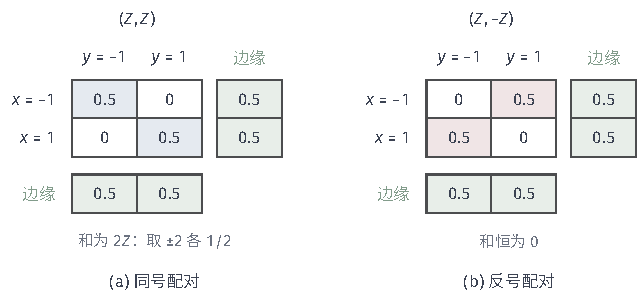
\includegraphics[width=108mm]{figures/02-abstract-mathematics/02-probability-spaces/tikz/wlim-joint-pairings/figure.pdf}
  \caption{边缘相同而联合分布不同的两种配对，$Z$以相等概率取$\pm1$。(a) $(Z,Z)$的联合概率表，质量在对角线上，坐标和为$2Z$。(b) $(Z,-Z)$的联合概率表，质量在反对角线上，坐标和恒为$0$。绿色单元是行边缘与列边缘，两种配对完全相同。}
  \label{fig:wlim-joint-pairings}
\end{figure}

\paragraph{Cram\'er--Wold判据}
联合分布的收敛可以化成一维问题，但要检验的不只是坐标，而是所有方向上的线性组合。

\begin{theorem}[\term{Cram\'er--Wold判据}]
\label{thm:wlim-cramer-wold}
设$\bm W_n,\bm W$是$\mathbb R^d$值随机向量。则$\bm W_n\Rightarrow\bm W$，当且仅当对每个$\bm a\in\mathbb R^d$都有$\bm a^\top\bm W_n\Rightarrow\bm a^\top\bm W$。
\end{theorem}

\begin{proof}
若$\bm W_n\Rightarrow\bm W$，对一维有界连续函数$h$，$\bm x\mapsto h(\bm a^\top\bm x)$在$\mathbb R^d$上有界连续，所以$\mathbb E\,h(\bm a^\top\bm W_n)\to\mathbb E\,h(\bm a^\top\bm W)$。
反过来，对每个$\bm a$，由一维弱收敛推出特征函数在$s=1$处收敛（定理~\ref{thm:wlim-levy}第一条）：
\[
  \varphi_{\bm W_n}(\bm a)=\mathbb E\,e^{i\bm a^\top\bm W_n}=\varphi_{\bm a^\top\bm W_n}(1)\to\varphi_{\bm a^\top\bm W}(1)=\varphi_{\bm W}(\bm a).
\]
所以向量特征函数逐点收敛到$\varphi_{\bm W}$，后者在原点连续。由定理~\ref{thm:wlim-levy}第二条，$\bm W_n$弱收敛到特征函数为$\varphi_{\bm W}$的分布，由唯一性这正是$\bm W$的分布。
\end{proof}

“所有方向”包括坐标的各种线性组合，只检验坐标方向不够。例~\ref{ex:wlim-alternating-pairing}中两个坐标方向的投影$X_n$与$Y_n$的分布都不变，但方向$\bm a=(1,1)$的投影$X_n+Y_n$不收敛。

\paragraph{行内独立时的乘积极限}
有一种常见情形无须逐个方向检验：同一行内的两组变量相互独立。

\begin{theorem}[行内独立的联合极限]
\label{thm:wlim-independent-product}
设对每个$n$，$\mathbb R^p$值的$\bm X_n$与$\mathbb R^q$值的$\bm Y_n$定义在同一概率空间上且相互独立。若$\bm X_n\Rightarrow P$、$\bm Y_n\Rightarrow Q$，则$(\bm X_n,\bm Y_n)\Rightarrow P\otimes Q$。
\end{theorem}

\begin{proof}
对$\bm s\in\mathbb R^p$、$\bm t\in\mathbb R^q$，由行内独立，
\[
  \varphi_{(\bm X_n,\bm Y_n)}(\bm s,\bm t)=\mathbb E\,e^{i\langle\bm s,\bm X_n\rangle}\,\mathbb E\,e^{i\langle\bm t,\bm Y_n\rangle}\to\varphi_P(\bm s)\varphi_Q(\bm t).
\]
由Fubini定理，右端正是乘积测度$P\otimes Q$的特征函数，它在原点连续，由定理~\ref{thm:wlim-levy}即得。
\end{proof}

定理要求的是每一行内部的独立性，不要求不同的$n$之间独立。若想用极限随机向量表述，应在乘积空间上取具有边缘$P$与$Q$的一对独立向量；随意取两个分别服从$P$与$Q$的变量，不能自动视为独立。

\subsection{连续函数变换下的分布极限}

\paragraph{连续映射保持弱收敛}
有了联合分布的极限，下一步是把它代入函数。设$S,T$是度量空间，$g:S\to T$可测，$P$在$g$下的推前$g_\#P$就是$g(X)$的分布，其中$X\sim P$。

\begin{theorem}[\term{连续映射定理}]
\label{thm:wlim-continuous-mapping}
设$S,T$是度量空间，$g:S\to T$连续。若$P_n\Rightarrow P$，则$g_\#P_n\Rightarrow g_\#P$；用随机对象表述，$X_n\Rightarrow X$推出$g(X_n)\Rightarrow g(X)$。
\end{theorem}

\begin{proof}
对$h\in C_b(T)$，$h\circ g\in C_b(S)$。由推前积分公式（式~\eqref{eq:measure-pushforward-integral}），
\[
  \int h\,d(g_\#P_n)=\int h\circ g\,dP_n\to\int h\circ g\,dP=\int h\,d(g_\#P),
\]
中间的极限来自$P_n\Rightarrow P$。
\end{proof}

证明中有界性由外层的$h$提供，所以$g$本身不必有界，例如$g(\bm x)=\lVert\bm x\rVert^2$。
坐标投影、范数和固定矩阵$\bm B$给出的线性变换$\bm x\mapsto\bm B\bm x$都是连续映射。对多个随机量，处理顺序总是先得到联合分布的极限，再代入连续函数：例如由$(X_n,Y_n)\Rightarrow(X,Y)$推出$X_n+Y_n\Rightarrow X+Y$、$X_nY_n\Rightarrow XY$；只有两个边缘的极限时，这一步无从谈起。

\paragraph{不连续点为零测集的映射}
阈值函数、比值等常用映射并非处处连续。只要不连续点在极限分布下概率为零，结论仍然成立。
记$D_g$为$g$的不连续点全体。它是Borel集：令$A_{m,k}$为满足“存在$y,z\in B(x,1/k)$使$d(g(y),g(z))\geq1/m$”的点$x$的集合，它是开集，而$D_g=\bigcup_m\bigcap_kA_{m,k}$。

\begin{theorem}[不连续点为零测集的连续映射]
\label{thm:wlim-continuous-mapping-ae}
设$g:S\to T$是Borel可测映射，$P_n\Rightarrow P$且$P(D_g)=0$，则$g_\#P_n\Rightarrow g_\#P$。
\end{theorem}

\begin{proof}
设$F\subseteq T$是闭集。若$x$属于$g^{-1}(F)$的闭包且$x\notin D_g$，取$x_k\in g^{-1}(F)$使$x_k\to x$，则$g(x_k)\to g(x)$，$F$闭推出$g(x)\in F$。所以$\overline{g^{-1}(F)}\subseteq g^{-1}(F)\cup D_g$。由定理~\ref{thm:wlim-portmanteau}，
\[
  \begin{aligned}
  \limsup_nP_n\bigl(g^{-1}(F)\bigr)&\leq\limsup_nP_n\bigl(\overline{g^{-1}(F)}\bigr)\leq P\bigl(\overline{g^{-1}(F)}\bigr)\\
  &\leq P\bigl(g^{-1}(F)\bigr)+P(D_g)=P\bigl(g^{-1}(F)\bigr).
  \end{aligned}
\]
即$\limsup_ng_\#P_n(F)\leq g_\#P(F)$，再用一次定理~\ref{thm:wlim-portmanteau}。
\end{proof}

以阈值函数$g(x)=\mathbb I_{\{x>c\}}$为例，$D_g=\{c\}$。若极限分布在$c$处没有原子，则$\mathbb I_{\{X_n>c\}}\Rightarrow\mathbb I_{\{X>c\}}$，即$\mathbb P(X_n>c)\to\mathbb P(X>c)$。
移动点质量$\delta_{1/n}$取$c=0$时这一条件失败：每个$\delta_{1/n}$在$0$处都没有原子，但极限$\delta_0$有；此时$\mathbb I_{\{1/n>0\}}=1$，而$\mathbb I_{\{0>0\}}=0$。条件必须对极限分布检查，只检查各个$P_n$不够。
本小节的映射$g$始终固定；随$n$变化的随机系数要先并入联合变量，下一小节处理这种情形。

\subsection{随机组合与标准化}

\paragraph{与常数配对的联合极限}
学生化均值的分母是样本标准差，它依概率趋于常数$\sigma$。这时不必另外研究联合分布：与一个趋于常数的量配对，联合极限自动确定。

\begin{theorem}[与常数配对的联合极限]
\label{thm:wlim-joint-constant}
设对每个$n$，$\mathbb R^p$值的$\bm X_n$与$\mathbb R^q$值的$\bm Y_n$定义在同一概率空间上。若$\bm X_n\Rightarrow\bm X$，并且对常向量$\bm c$及每个$\varepsilon>0$有$\mathbb P(\lVert\bm Y_n-\bm c\rVert>\varepsilon)\to0$，则$(\bm X_n,\bm Y_n)\Rightarrow(\bm X,\bm c)$。
\end{theorem}

\begin{proof}
设$h\in C_b(\mathbb R^{p+q})$，$|h|\leq M$，固定$\varepsilon>0$。由引理~\ref{lem:wlim-convergent-tight}，取紧集$K\subseteq\mathbb R^p$使$\mathbb P(\bm X_n\notin K)<\varepsilon$对所有$n$成立。
$h$在紧集$K\times\overline B(\bm c,1)$上一致连续，取$\eta\in(0,1]$，使$\bm x\in K$、$\lVert\bm y-\bm c\rVert\leq\eta$时$|h(\bm x,\bm y)-h(\bm x,\bm c)|<\varepsilon$。在事件$\{\bm X_n\in K,\ \lVert\bm Y_n-\bm c\rVert\leq\eta\}$之外，差值不超过$2M$，于是
\[
  \bigl|\mathbb E\,h(\bm X_n,\bm Y_n)-\mathbb E\,h(\bm X_n,\bm c)\bigr|\leq\varepsilon+2M\bigl[\varepsilon+\mathbb P(\lVert\bm Y_n-\bm c\rVert>\eta)\bigr].
\]
方括号中第二项趋于零。另一方面$\bm x\mapsto h(\bm x,\bm c)$有界连续，$\mathbb E\,h(\bm X_n,\bm c)\to\mathbb E\,h(\bm X,\bm c)$。合并得$\limsup_n|\mathbb E\,h(\bm X_n,\bm Y_n)-\mathbb E\,h(\bm X,\bm c)|\leq\varepsilon+2M\varepsilon$，而$\varepsilon$任意。
\end{proof}

证明只控制$\bm Y_n$偏离常量的概率，不要求$\bm X_n$与$\bm Y_n$独立；不同的$n$也可以使用不同的概率空间，只要求同一行内的$\bm X_n$与$\bm Y_n$共同定义。

\paragraph{Slutsky规则}
把加法、乘法和除法作为联合极限上的映射，就得到最常用的组合规则。

\begin{theorem}[\term{Slutsky定理}]
\label{thm:wlim-slutsky}
在定理~\ref{thm:wlim-joint-constant}的条件下：
\begin{enumerate}
  \item 若$p=q$，则$\bm X_n+\bm Y_n\Rightarrow\bm X+\bm c$；
  \item 若$\bm Y_n$是$m\times p$随机矩阵（按坐标排成向量），常矩阵为$\bm C$，则$\bm Y_n\bm X_n\Rightarrow\bm C\bm X$；特别地，实值$Y_n\to c$时$Y_n\bm X_n\Rightarrow c\bm X$；
  \item 若$Y_n$实值、$c\neq0$，在$\{Y_n=0\}$上把商任意规定为$\bm 0$，则$\bm X_n/Y_n\Rightarrow\bm X/c$。
\end{enumerate}
\end{theorem}

\begin{proof}
前两条中的加法与矩阵乘法是连续映射，对定理~\ref{thm:wlim-joint-constant}给出的联合极限应用定理~\ref{thm:wlim-continuous-mapping}。
第三条中映射$g(\bm x,y)=\bm x/y$（$y\neq0$）、$g(\bm x,0)=\bm 0$的不连续点含于$\{y=0\}$，而极限$(\bm X,c)$落在其中的概率为零，由定理~\ref{thm:wlim-continuous-mapping-ae}即得。
另外$\mathbb P(Y_n=0)\leq\mathbb P(|Y_n-c|\geq|c|)\to0$，所以商在$\{Y_n=0\}$上怎样规定不影响结论。
\end{proof}

\paragraph{学生化的样本均值}
Slutsky规则最典型的用途是用估计的尺度替换未知尺度。同一批数据同时产生分子和分母，二者并不独立，这不妨碍使用规则。

\begin{example}[学生化均值]
\label{ex:wlim-studentized-mean}
设$X_1,X_2,\ldots$独立同分布，均值$\mu$，方差$0<\sigma^2<\infty$，$S_n^2=\frac1{n-1}\sum_{k=1}^n(X_k-\bar X_n)^2$。
由强大数定律（定理~\ref{thm:conv-slln}），$\frac1n\sum_kX_k^2\to\mathbb E X_1^2$与$\bar X_n\to\mu$几乎必然成立，于是
\[
  S_n^2=\frac n{n-1}\Bigl(\frac1n\sum_{k=1}^nX_k^2-\bar X_n^2\Bigr)\to\mathbb E X_1^2-\mu^2=\sigma^2
\]
几乎必然成立，从而依概率成立（定理~\ref{thm:conv-implications}）；平方根连续，$S_n\to\sigma$依概率成立。
若已知$\sqrt n(\bar X_n-\mu)\Rightarrow N(0,\sigma^2)$（第~\ref{sec:wlim-clt}节将证明），由Slutsky规则第三条，
\[
  \frac{\sqrt n(\bar X_n-\mu)}{S_n}\Rightarrow\frac1\sigma N(0,\sigma^2)=N(0,1).
\]
\end{example}

图~\ref{fig:wlim-studentized-shift}(a)用指数总体模拟学生化均值的经验分布函数。$n=5$时左尾明显偏重，与$\Phi$的最大差约为$0.16$；$n=20$与$n=100$时这一差距约为$0.076$与$0.034$。
左尾偏重的原因是指数分布右偏：样本均值偏小的样本往往样本标准差也偏小，分子与分母同时变小，商被推向更负的值。Slutsky规则说明这种依赖在极限中消失，但没有给出有限样本中消失得多快。

\begin{figure}[htbp]
  \centering
  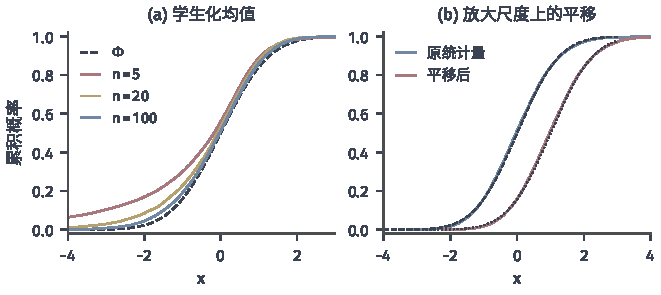
\includegraphics[width=112mm]{figures/02-abstract-mathematics/02-probability-spaces/matplotlib/wlim-studentized-shift/figure.pdf}
  \caption{随机标准化与尺度下的平移。总体为率参数$1$的指数分布，固定随机种子，每条曲线基于$20000$次重复。(a) 学生化均值$\sqrt n(\bar X_n-1)/S_n$的经验分布函数，$n=5,20,100$，虚线为$\Phi$。(b) $n=100$时$\sqrt n(\bar X_n-1)$（蓝）与把$\bar X_n$平移$1/\sqrt n=0.1$后的$\sqrt n(\bar X_n+1/\sqrt n-1)$（红）的经验分布函数，虚线与点线分别为$\Phi(x)$与$\Phi(x-1)$。}
  \label{fig:wlim-studentized-shift}
\end{figure}

\subsection{近似替换与渐近等价}

\paragraph{逐行可比较的近似量}
实际计算中常把一个统计量换成更容易处理的近似量，例如用分母$n$代替$n-1$，或删去一个高阶小项。替换是否改变分布极限，取决于两者的差是否依概率趋于零。

\begin{theorem}[近似替换]
\label{thm:wlim-approximation}
设对每个$n$，$\mathbb R^d$值的$\bm X_n$与$\widetilde{\bm X}_n$定义在同一概率空间上。若$\bm X_n\Rightarrow\bm X$，且$\lVert\widetilde{\bm X}_n-\bm X_n\rVert\to0$依概率成立，则$\widetilde{\bm X}_n\Rightarrow\bm X$。
\end{theorem}

\begin{proof}
写$\widetilde{\bm X}_n=\bm X_n+(\widetilde{\bm X}_n-\bm X_n)$，第二项依概率趋于常向量$\bm 0$，由Slutsky规则第一条即得。
\end{proof}

满足定理条件的两列称为渐近等价。一个易于检验的特例是$\mathbb P(\widetilde{\bm X}_n\neq\bm X_n)\to0$，因为$\mathbb P(\lVert\widetilde{\bm X}_n-\bm X_n\rVert>\varepsilon)\leq\mathbb P(\widetilde{\bm X}_n\neq\bm X_n)$。
定理的前提是二者能逐行比较。若只知道$\bm X_n$与$\widetilde{\bm X}_n$各自的分布，差$\widetilde{\bm X}_n-\bm X_n$连定义都没有，替换无从谈起。

\paragraph{缩放尺度下的误差}
替换条件必须在实际使用的尺度上检验。设$a_n>0$是确定的缩放系数，$\theta$是固定中心，已知$a_n(T_n-\theta)\Rightarrow L$。要用$\widetilde T_n$替换$T_n$，应验证
\[
  a_n(\widetilde T_n-T_n)\to0\quad\text{依概率成立},
\]
这时$a_n(\widetilde T_n-\theta)=a_n(T_n-\theta)+a_n(\widetilde T_n-T_n)\Rightarrow L$。仅有$\widetilde T_n-T_n\to0$不够。

最简单的反例是确定的平移。令$\widetilde T_n=T_n+1/\sqrt n$，差$1/\sqrt n$在原尺度上趋于零；但在$\sqrt n$尺度上，$\sqrt n(\widetilde T_n-T_n)=1$恒成立，极限整体平移一个单位。
图~\ref{fig:wlim-studentized-shift}(b)以$n=100$的指数样本均值为例：原尺度上的平移只有$0.1$，放大后的两条经验分布函数却分别贴近$\Phi(x)$与$\Phi(x-1)$。
统计模型中估计量的具体误差展开与Delta方法，在\BookPartRef{part:inference-and-causal-identification}{卷四“推断与因果识别”部分}展开；这里只保留通用的替换规则。

\section{标准化部分和的分布极限}
\label{sec:wlim-clt}

第~\ref{chap:random-variable-convergence}章研究了独立部分和是否收敛、样本平均是否靠近期望。本节研究另一个问题：把部分和中心化，再按它的波动尺度缩放，所得分布是否有稳定的极限。
我们按求和项满足的条件依次处理独立同分布、独立非同分布和随机向量三种情形。证明都使用第~\ref{sec:wlim-characteristic}节的特征函数，随机标准化与线性变换使用第~\ref{sec:wlim-joint-transform}节的规则。

\subsection{独立同分布情形}

\paragraph{特征函数的乘积极限}
标准化和的特征函数是$n$个相同因子的乘积。要比较两个乘积，下面的估计把乘积之差化成因子之差的和。

\begin{lemma}[乘积之差]
\label{lem:wlim-product-difference}
设复数$z_1,\ldots,z_n$与$w_1,\ldots,w_n$的模都不超过$1$，则
\[
  \Bigl|\prod_{k=1}^nz_k-\prod_{k=1}^nw_k\Bigr|\leq\sum_{k=1}^n|z_k-w_k|.
\]
\end{lemma}

\begin{proof}
对$n$归纳。$n=1$时显然成立。由
\[
  \prod_{k\leq n}z_k-\prod_{k\leq n}w_k=z_n\Bigl(\prod_{k<n}z_k-\prod_{k<n}w_k\Bigr)+(z_n-w_n)\prod_{k<n}w_k,
\]
以及$|z_n|\leq1$、$|\prod_{k<n}w_k|\leq1$，由归纳假设即得。
\end{proof}

\begin{theorem}[独立同分布的\term{中心极限定理}]
\label{thm:wlim-clt-iid}
设$X_1,X_2,\ldots$独立同分布，$\mathbb E X_1=\mu$，$0<\sigma^2=\operatorname{Var}X_1<\infty$。令
\[
  T_n=\frac{\sum_{k=1}^nX_k-n\mu}{\sigma\sqrt n}.
\]
则$T_n\Rightarrow N(0,1)$。
\end{theorem}

\begin{proof}
令$Y_k=(X_k-\mu)/\sigma$，它们独立同分布，均值为$0$，方差为$1$，$T_n=\sum_kY_k/\sqrt n$。由定理~\ref{thm:wlim-chf-operations}，
\[
  \varphi_{T_n}(t)=\Bigl[\varphi_{Y_1}\Bigl(\frac t{\sqrt n}\Bigr)\Bigr]^n.
\]
固定$t$。当$n\geq t^2/2$时$0\leq1-t^2/(2n)\leq1$，对$z_k=\varphi_{Y_1}(t/\sqrt n)$、$w_k=1-t^2/(2n)$用引理~\ref{lem:wlim-product-difference}，
\[
  \Bigl|\varphi_{T_n}(t)-\Bigl(1-\frac{t^2}{2n}\Bigr)^n\Bigr|\leq n\Bigl|\varphi_{Y_1}\Bigl(\frac t{\sqrt n}\Bigr)-1+\frac{t^2}{2n}\Bigr|.
\]
由定理~\ref{thm:wlim-chf-second-order}，$\varphi_{Y_1}(u)-1+u^2/2=o(u^2)$，取$u=t/\sqrt n$，右端是$n\cdot o(t^2/n)\to0$。又$(1-t^2/(2n))^n\to e^{-t^2/2}$，所以$\varphi_{T_n}(t)\to e^{-t^2/2}$。
极限是$N(0,1)$的特征函数（式~\eqref{eq:wlim-normal-chf}），在原点连续，由L\'evy连续性定理得$T_n\Rightarrow N(0,1)$。
\end{proof}

证明只用到有限二阶矩。条件$\sigma^2>0$不能省：若$\sigma^2=0$，各项几乎必然等于$\mu$，中心化部分和恒为零，含$1/\sigma$的标准化公式没有意义。

图~\ref{fig:wlim-clt-convergence}以指数总体为例检查定理。$n$个率参数为$1$的指数变量之和服从Gamma分布，$T_n$的分布函数可以精确计算。
(a)中$n=1$的分布函数在$-1$以下为零，形状明显偏斜；$n=16$与$n=64$时已经接近$\Phi$。(c)对应证明本身：特征函数$[\varphi_{Y_1}(t/\sqrt n)]^n$的实部随$n$增大贴近$e^{-t^2/2}$。

(b)记录分布函数的最大偏差$\sup_x|\mathbb P(T_n\leq x)-\Phi(x)|$：指数总体从$n=1$时的$0.159$降到$n=1000$时的$0.0042$，Bernoulli$(0.2)$总体从$0.49$降到$0.019$。两条点列在双对数坐标中都近似平行于斜率$-1/2$的参考线；Bernoulli总体的偏差更大，因为它是格点分布，分布函数始终有跳跃。
这些是对两个具体总体的观察。中心极限定理本身只断言偏差趋于零，不给出任何固定$n$下的误差界；讨论近似速度需要附加矩条件和专门的误差定理。

\begin{figure*}[htbp]
  \centering
  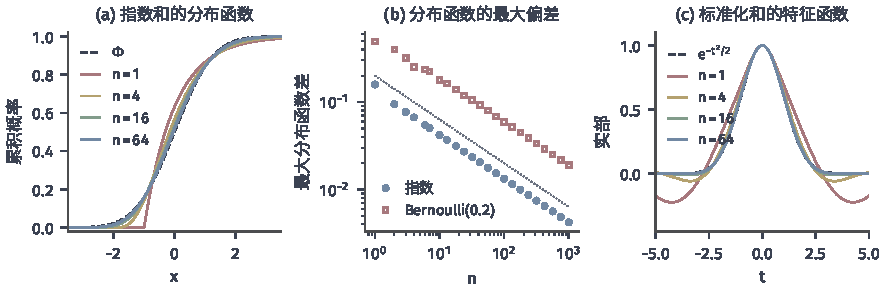
\includegraphics[width=150mm]{figures/02-abstract-mathematics/02-probability-spaces/matplotlib/wlim-clt-convergence/figure.pdf}
  \caption{标准化和向标准正态分布收敛。(a) 率参数$1$的指数总体，$T_n=(S_n-n)/\sqrt n$的精确分布函数（$S_n$服从形状$n$、率$1$的Gamma分布），$n=1,4,16,64$，虚线为$\Phi$。(b) 指数总体与$\operatorname{Bernoulli}(0.2)$总体的最大分布函数偏差，双对数坐标，点线为参考线$0.2/\sqrt n$。(c) 指数总体中心化后$\varphi_{Y_1}(u)=e^{-iu}/(1-iu)$，标准化和的特征函数$[\varphi_{Y_1}(t/\sqrt n)]^n$的实部与$e^{-t^2/2}$（虚线）。}
  \label{fig:wlim-clt-convergence}
\end{figure*}

\paragraph{样本平均的误差分布}
由连续映射$x\mapsto\sigma x$，定理~\ref{thm:wlim-clt-iid}等价于
\begin{equation}
  \sqrt n(\bar X_n-\mu)\Rightarrow N(0,\sigma^2).
  \label{eq:wlim-clt-mean}
\end{equation}
它与强大数定律（定理~\ref{thm:conv-slln}）回答不同的问题。大数定律说明$\bar X_n$几乎必然趋于$\mu$，即平均值最终停在哪里；式~\eqref{eq:wlim-clt-mean}把误差$\bar X_n-\mu$放大$\sqrt n$倍，说明放大后的波动具有什么形状。前者是同一概率空间上的逐样本结论，后者只涉及分布。

\BookChapterRef{chap:sampling-errors}{卷一“抽样分布与估计误差”章}陈述了中心极限定理并用它构造正态近似；本节在一般有限方差条件下给出了证明。
用样本标准差$S_n$替换$\sigma$时，例~\ref{ex:wlim-studentized-mean}已经说明，只需$S_n\to\sigma$依概率成立，再由Slutsky规则得到$\sqrt n(\bar X_n-\mu)/S_n\Rightarrow N(0,1)$，不需要分子与分母独立。

\subsection{独立非同分布情形}

\paragraph{三角阵与Lindeberg条件}
许多误差由不同来源、不同权重的项累加而成，例如加权平均$\sum_kw_k\varepsilon_k$中权重随样本量重新分配。这时求和项不再同分布，甚至每一行的项都随$n$改变。
我们把它们写成三角阵：对每个$n$，$X_{n,1},\ldots,X_{n,m_n}$同一行内相互独立，均值为零，方差有限，记
\[
  s_n^2=\sum_{k=1}^{m_n}\mathbb E X_{n,k}^2\in(0,\infty),\qquad T_n=\frac1{s_n}\sum_{k=1}^{m_n}X_{n,k}.
\]
均值不为零的项要先中心化。同一行内要求独立，不同行之间不作任何要求，各行甚至可以定义在不同的概率空间上。

\begin{definition}[\term{Lindeberg条件}]
\label{def:wlim-lindeberg-condition}
称上述三角阵满足Lindeberg条件，若对每个$\varepsilon>0$，
\[
  L_n(\varepsilon)=\frac1{s_n^2}\sum_{k=1}^{m_n}\mathbb E\bigl[X_{n,k}^2\,\mathbb I_{\{|X_{n,k}|>\varepsilon s_n\}}\bigr]\to0.
\]
\end{definition}

\begin{theorem}[Lindeberg中心极限定理]
\label{thm:wlim-lindeberg}
设三角阵$X_{n,k}$每行独立、均值为零、$s_n^2\in(0,\infty)$，并满足Lindeberg条件，则$T_n\Rightarrow N(0,1)$。
\end{theorem}

\paragraph{条件的含义}
$L_n(\varepsilon)$度量的是超出整体波动尺度$\varepsilon s_n$的那部分取值对总方差的贡献。条件要求这部分贡献在总方差中的比例趋于零，即和中没有哪一项能以不可忽略的方差份额单独产生大偏差。
由此还能推出每一项的方差占比一致趋于零：把$\mathbb E X_{n,k}^2$拆成$|X_{n,k}|\leq\varepsilon s_n$与$|X_{n,k}|>\varepsilon s_n$两部分，前者不超过$\varepsilon^2s_n^2$，于是
\begin{equation}
  \max_k\frac{\mathbb E X_{n,k}^2}{s_n^2}\leq\varepsilon^2+L_n(\varepsilon),
  \label{eq:wlim-max-share}
\end{equation}
先令$n\to\infty$，再令$\varepsilon\to0$，得最大方差占比趋于零。

独立同分布情形是特例：取$X_{n,k}=X_k-\mu$、$m_n=n$，则$s_n^2=n\sigma^2$，
\[
  L_n(\varepsilon)=\frac1{\sigma^2}\mathbb E\bigl[(X_1-\mu)^2\,\mathbb I_{\{|X_1-\mu|>\varepsilon\sigma\sqrt n\}}\bigr]\to0,
\]
因为被积函数逐点趋于零且以可积的$(X_1-\mu)^2$为界。

\paragraph{Lindeberg定理的证明}
证明沿用同分布情形的路线，只是每个因子不同，需要把小偏差与大偏差分开估计。

\begin{proof}[定理~\ref{thm:wlim-lindeberg}的证明]
记$Y_{n,k}=X_{n,k}/s_n$、$\sigma_{n,k}^2=\mathbb E Y_{n,k}^2$，则$\sum_k\sigma_{n,k}^2=1$，由式~\eqref{eq:wlim-max-share}有$\max_k\sigma_{n,k}^2\to0$。固定$t$，由行内独立，$\varphi_{T_n}(t)=\prod_k\varphi_{Y_{n,k}}(t)$。

第一步，与二次近似比较。由引理~\ref{lem:wlim-exp-remainder}，在$\{|Y_{n,k}|\leq\varepsilon\}$上用三阶界，在其补集上用二阶界：
\[
  \begin{aligned}
  \Bigl|\varphi_{Y_{n,k}}(t)-1+\frac{t^2\sigma_{n,k}^2}2\Bigr|
  &\leq\frac{|t|^3}6\mathbb E\bigl[|Y_{n,k}|^3\mathbb I_{\{|Y_{n,k}|\leq\varepsilon\}}\bigr]+t^2\,\mathbb E\bigl[Y_{n,k}^2\mathbb I_{\{|Y_{n,k}|>\varepsilon\}}\bigr]\\
  &\leq\frac{|t|^3\varepsilon}6\sigma_{n,k}^2+t^2\,\mathbb E\bigl[Y_{n,k}^2\mathbb I_{\{|Y_{n,k}|>\varepsilon\}}\bigr].
  \end{aligned}
\]
对$k$求和，右端之和不超过$|t|^3\varepsilon/6+t^2L_n(\varepsilon)$。当$n$充分大时$t^2\max_k\sigma_{n,k}^2\leq2$，各个$1-t^2\sigma_{n,k}^2/2$落在$[0,1]$中，由引理~\ref{lem:wlim-product-difference}，
\[
  \limsup_n\Bigl|\varphi_{T_n}(t)-\prod_k\Bigl(1-\frac{t^2\sigma_{n,k}^2}2\Bigr)\Bigr|\leq\frac{|t|^3\varepsilon}6,
\]
$\varepsilon$任意，所以左端极限为零。

第二步，与正态特征函数比较。记$x_k=t^2\sigma_{n,k}^2/2\geq0$，则$\prod_ke^{-x_k}=e^{-t^2/2}$。对$x\geq0$有$|e^{-x}-1+x|\leq x^2/2$，再用一次引理~\ref{lem:wlim-product-difference}，
\[
  \Bigl|\prod_k(1-x_k)-e^{-t^2/2}\Bigr|\leq\sum_k\frac{x_k^2}2\leq\frac12\Bigl(\max_kx_k\Bigr)\sum_kx_k=\frac{t^4}8\max_k\sigma_{n,k}^2\to0.
\]
两步合并得$\varphi_{T_n}(t)\to e^{-t^2/2}$，由L\'evy连续性定理即得结论。
\end{proof}

证明中Lindeberg条件起两个作用：在第一步直接控制大偏差项的二阶余项；经式~\eqref{eq:wlim-max-share}保证最大方差占比趋于零，使第一步的各个$1-t^2\sigma_{n,k}^2/2$落在$[0,1]$中，并使第二步的误差消失。小偏差项用三阶估计，但三阶矩只在$\{|Y_{n,k}|\leq\varepsilon\}$上出现，自然有界，所以定理不需要三阶矩。

\paragraph{Lyapunov条件与不等权误差}
Lindeberg条件需要计算截断二阶矩。较易检验的是下面的高阶矩条件：存在$\delta>0$使
\[
  \frac1{s_n^{2+\delta}}\sum_{k=1}^{m_n}\mathbb E|X_{n,k}|^{2+\delta}\to0,
\]
称为\term{Lyapunov条件}。在$\{|X_{n,k}|>\varepsilon s_n\}$上，$X_{n,k}^2\leq|X_{n,k}|^{2+\delta}/(\varepsilon s_n)^\delta$，逐项求和得$L_n(\varepsilon)\leq\varepsilon^{-\delta}s_n^{-2-\delta}\sum_k\mathbb E|X_{n,k}|^{2+\delta}\to0$，所以Lyapunov条件推出Lindeberg条件。
注意条件是一个比值的极限，“各项都有$2+\delta$阶矩”本身并不够。

\begin{example}[不等权的独立误差]
\label{ex:wlim-unequal-weights}
设$R_1,R_2,\ldots$独立，以相等概率取$\pm1$。
第一种方案取$X_{n,k}=kR_k$，$1\leq k\leq n$，即第$k$个误差的权重为$k$。此时$s_n^2=\sum_{k\leq n}k^2=n(n+1)(2n+1)/6$，最大方差占比$n^2/s_n^2\approx3/n\to0$。由于$|X_{n,k}|\leq n$而$s_n\geq n^{3/2}/\sqrt3$，当$n>3/\varepsilon^2$时没有任何项超过$\varepsilon s_n$，$L_n(\varepsilon)=0$；Lindeberg条件成立，$T_n\Rightarrow N(0,1)$。
第二种方案让首项主导：$X_{n,1}=2\sqrt{n-1}\,R_1$，$X_{n,k}=R_k$（$2\leq k\leq n$）。此时$s_n^2=5(n-1)$，首项的方差占比恒为$4/5$；当$\varepsilon<2/\sqrt5$时首项总超过$\varepsilon s_n$，$L_n(\varepsilon)\geq4/5$，Lindeberg条件不成立。
事实上$T_n=\bigl(2R_1+\sum_{k\geq2}R_k/\sqrt{n-1}\bigr)/\sqrt5$。由定理~\ref{thm:wlim-clt-iid}，括号中的第二项依分布收敛到$N(0,1)$，且它与$R_1$在同一行内独立；由定理~\ref{thm:wlim-independent-product}与连续映射，$T_n\Rightarrow(2R+G)/\sqrt5$，其中$R$与$G\sim N(0,1)$独立。这一极限方差为$1$，却是$N(\pm2/\sqrt5,1/5)$的等权混合，不是正态分布。
\end{example}

图~\ref{fig:wlim-lindeberg-triangular}对照两种方案。(a)中递增权重方案的最大方差占比按$3/n$的量级下降，主导首项方案停在$4/5$。(b)中$n=200$时，前者的行和直方图贴合标准正态密度，后者呈现以$\pm2/\sqrt5\approx\pm0.89$为中心的双峰，与混合正态密度一致。
三角阵的用途正在于此：权重和参与求和的项随$n$变化时，必须对每一行重新计算总方差和各项的相对贡献，而不能沿用同分布情形的结论。
在最大方差占比趋于零的前提下，Lindeberg条件也是正态极限的必要条件（Feller定理），本章不证明这一方向。

\begin{figure}[htbp]
  \centering
  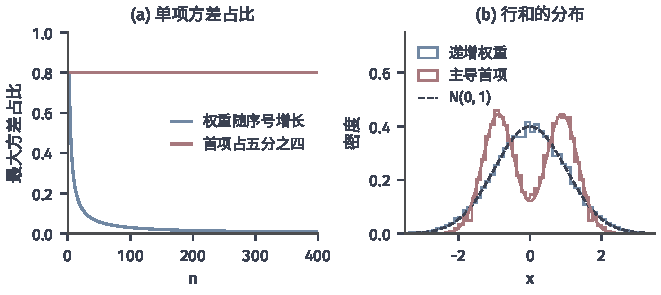
\includegraphics[width=112mm]{figures/02-abstract-mathematics/02-probability-spaces/matplotlib/wlim-lindeberg-triangular/figure.pdf}
  \caption{三角阵中单项方差占比与行和的分布，$R_k$为独立的Rademacher变量。(a) 最大方差占比$\max_k\mathbb E X_{n,k}^2/s_n^2$：权重$X_{n,k}=kR_k$时为$6n/((n+1)(2n+1))$；首项$X_{n,1}=2\sqrt{n-1}R_1$主导时恒为$4/5$。(b) $n=200$时两种方案的行和$T_n$的直方图（固定随机种子，$20000$次重复），虚线为$N(0,1)$密度，红色实线为主导首项方案的极限密度，即$N(\pm2/\sqrt5,1/5)$的等权混合。}
  \label{fig:wlim-lindeberg-triangular}
\end{figure}

\subsection{随机向量情形}

\paragraph{逐方向的标量极限}
许多统计量同时包含几个样本平均，例如样本均值与样本二阶矩，我们需要它们的联合误差分布。Cram\'er--Wold判据把这个问题化为每个方向上的一维中心极限定理。

\begin{theorem}[多维中心极限定理]
\label{thm:wlim-clt-vector}
设$\bm X_1,\bm X_2,\ldots$是独立同分布的$\mathbb R^d$值随机向量，均值为$\bm\mu$，协方差矩阵$\bm\Sigma$有限。则
\[
  \sqrt n(\bar{\bm X}_n-\bm\mu)\Rightarrow N(\bm 0,\bm\Sigma).
\]
\end{theorem}

\begin{proof}
固定$\bm a\in\mathbb R^d$。单项投影$\bm a^\top(\bm X_k-\bm\mu)$独立同分布，均值为零，方差为$\bm a^\top\bm\Sigma\bm a$。
若$\bm a^\top\bm\Sigma\bm a>0$，由定理~\ref{thm:wlim-clt-iid}与式~\eqref{eq:wlim-clt-mean}，$\bm a^\top\sqrt n(\bar{\bm X}_n-\bm\mu)\Rightarrow N(0,\bm a^\top\bm\Sigma\bm a)$。
若$\bm a^\top\bm\Sigma\bm a=0$，各项投影几乎必然为零，$\bm a^\top\sqrt n(\bar{\bm X}_n-\bm\mu)=0$几乎必然成立，同样收敛到$N(0,0)=\delta_0$。
另一方面，若$\bm W\sim N(\bm 0,\bm\Sigma)$，由式~\eqref{eq:wlim-mvn-chf}，$\varphi_{\bm a^\top\bm W}(s)=\varphi_{\bm W}(s\bm a)=e^{-s^2\bm a^\top\bm\Sigma\bm a/2}$，所以$\bm a^\top\bm W\sim N(0,\bm a^\top\bm\Sigma\bm a)$。由Cram\'er--Wold判据即得结论。
\end{proof}

\paragraph{奇异协方差与线性变换}
定理只要求$\bm\Sigma$半正定，不要求可逆，因而不依赖于白化或密度。$\bm\Sigma$奇异时，存在方向$\bm a\neq\bm 0$使$\bm a^\top\bm\Sigma\bm a=0$，极限分布集中在与这些方向正交的低维子空间上。
对固定的$m\times d$矩阵$\bm B$，由连续映射定理与式~\eqref{eq:wlim-mvn-chf}，
\[
  \bm B\sqrt n(\bar{\bm X}_n-\bm\mu)\Rightarrow N(\bm 0,\bm B\bm\Sigma\bm B^\top),
\]
所以联合极限同时给出任意有限个线性组合的联合波动。

图~\ref{fig:wlim-clt-vector}以$\xi\sim$率参数$1$的指数分布为例。(a)取$\bm X=(\xi,\xi^2)$，均值$(1,2)$，由$\mathbb E\xi^3=6$、$\mathbb E\xi^4=24$得
\[
  \bm\Sigma=\begin{pmatrix}1&4\\4&20\end{pmatrix};
\]
$n=200$时$1500$个$\sqrt n(\bar{\bm X}_n-\bm\mu)$的散点沿$\bm\Sigma$的主轴方向伸展，与$N(\bm 0,\bm\Sigma)$的$95\%$概率椭圆相符，样本协方差约为$\begin{pmatrix}1.01&4.13\\4.13&20.8\end{pmatrix}$。
(b)给出两个方向的投影：$\bm a=(1,0)$的极限方差为$1$，$\bm a=(1,-0.2)$的极限方差为$1-1.6+0.8=0.2$，直方图分别贴合相应的正态密度。后一个方向几乎与长轴垂直，波动远小于任一坐标，这正是只看坐标无法得到的信息。
(c)取$\bm X=(\xi,3-2\xi)$，$\bm\Sigma=\begin{pmatrix}1&-2\\-2&4\end{pmatrix}$的秩为一，方向$\bm a=(2,1)$上的方差为零，所有散点都落在直线$V_2=-2V_1$上；极限$N(\bm 0,\bm\Sigma)$集中在同一条直线上，没有二维密度。

\begin{figure*}[htbp]
  \centering
  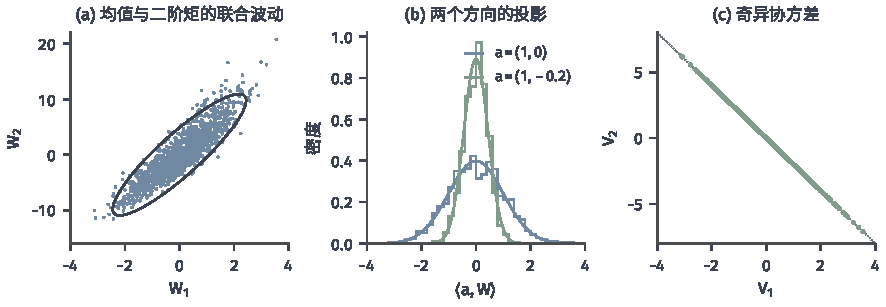
\includegraphics[width=150mm]{figures/02-abstract-mathematics/02-probability-spaces/matplotlib/wlim-clt-vector/figure.pdf}
  \caption{二维中心极限定理，$\xi$服从率参数$1$的指数分布，$n=200$，固定随机种子，$1500$次重复。(a) $\bm W=\sqrt n(\bar{\bm X}_n-\bm\mu)$，$\bm X=(\xi,\xi^2)$，实线为$N(\bm 0,\bm\Sigma)$的$95\%$概率椭圆，$\bm\Sigma=\bigl(\begin{smallmatrix}1&4\\4&20\end{smallmatrix}\bigr)$。(b) $\bm W$沿$\bm a=(1,0)$与$\bm a=(1,-0.2)$的投影直方图，实线为极限密度$N(0,1)$与$N(0,0.2)$。(c) $\bm X=(\xi,3-2\xi)$时的$\bm V=\sqrt n(\bar{\bm X}_n-\bm\mu)$，协方差矩阵秩为一，点全部落在直线$V_2=-2V_1$（点线）上。}
  \label{fig:wlim-clt-vector}
\end{figure*}

这里的维数$d$固定，结论属于有限维分布理论。把部分和看成随时间变化的整条路径，并研究路径的分布极限，需要路径空间上的紧性，留给\BookPartRef{part:dynamical-systems-control-decision-and-games}{卷三“过程与轨迹演化”部分}。

\section{本章小结}
\label{sec:wlim-summary}

章首的模拟研究中，不同样本量的数据分别生成，只能比较分布。本章的回答是：$T_n$的分布趋近$N(0,1)$，意思是每个有界连续函数的平均值都收敛，在实轴上等价于分布函数在极限的连续点处收敛。
由此能直接读出边界零质量事件的概率极限；闭集与开集只有单向不等式；均值、矩等无界积分还需要一致可积这一尾部条件，尖峰分布说明弱收敛本身不控制它。弱收敛只记录分布，不记录配对，所以它推不出依概率收敛，极限为常数时才是例外。

本章区分了围绕分布列的四类任务。给定候选极限时检验收敛，用测试函数或Portmanteau判据；没有候选极限时取得子列，靠一致紧性与Prokhorov定理；识别子列极限，靠特征函数的唯一性与L\'evy连续性定理；对几个随机量作运算，先由Cram\'er--Wold判据、行内独立或与常数配对得到联合极限，再用连续映射、Slutsky规则与近似替换传递极限。
各个条件分管不同的风险：一致紧性防止质量逃到紧集之外，一致可积防止无界积分的尾部贡献，事件边界、映射不连续点与随机分母的零点各有自己的零测条件，不能用一种控制代替其余。

回到独立部分和，第~\ref{chap:random-variable-convergence}章的大数定律说明样本平均最终停在期望处，本章的中心极限定理刻画误差放大$\sqrt n$倍后的形状。
证明的核心是特征函数把独立和变成乘积，有限二阶矩给出二阶展开，乘积极限给出$e^{-t^2/2}$。Lindeberg条件把这一论证推广到每行内部独立、权重各异的三角阵，它要求没有哪一项占据不可忽略的方差份额；向量情形则由逐方向的一维结论与Cram\'er--Wold判据合成，协方差矩阵可以奇异。
这些结论都只涉及固定维数的分布，不提供有限样本误差界。比较分布的更强距离、估计量的渐近推断与整条随机路径的极限，分别在后续相应部分展开。

